\documentclass[a4paper]{book}
\usepackage{a4wide}
\usepackage{makeidx}
\usepackage{fancyhdr}
\usepackage{graphicx}
\usepackage{multicol}
\usepackage{float}
\usepackage{textcomp}
\usepackage{alltt}
\usepackage[utf8]{inputenc}
\usepackage{doxygen}
\makeindex
\setcounter{tocdepth}{3}
\renewcommand{\footrulewidth}{0.4pt}
\begin{document}
\begin{titlepage}
\vspace*{7cm}
\begin{center}
{\Large HPGS - HPGl Script }\\
\vspace*{1cm}
{\large Generated by Doxygen 1.5.6}\\
\vspace*{0.5cm}
{\small Wed Feb 11 16:49:40 2009}\\
\end{center}
\end{titlepage}
\clearemptydoublepage
\pagenumbering{roman}
\tableofcontents
\clearemptydoublepage
\pagenumbering{arabic}
\chapter{The HPGS documentation}
\label{index}\section{Introduction}\label{index_intro_sec}
HPGS has been developed by {\tt EV-i Informationstechnologie GmbH} and has been published under the {\tt LGPL}.

For Details visit the {\tt project's homepage}.\section{Installation}\label{index_install_sec}
See the file INSTALL of the distribution.\section{Invoking hpgs}\label{index_invoke_sec}


\begin{VerbInclude}\begin{verbatim}
 hpgs v1.1.5 - HPGl Script, a hpgl/2 interpreter/renderer.

 (C) 2004-2009 ev-i Informationstechnologie GmbH (http://www.ev-i.at)
     published under the LGPL (http://www.fsf.org/licenses/lgpl.html).

usage: hpgs [-i] [-v] [-q] [-d <dev>] [options...] [-o <out>] <in1> <in2>...
       -i ... Ignore plotsize from PS and determine
              the plotsize from the file content.
       --linewidth-size ... Account for linewidths in the plotsize
              calculation for -i (default behaviour).
       --no-linewidth-size ... Ignore linewidths in the plotsize
              calculation for -i.
       -v ... Increase verbosity.
       -q ... Decrease verbosity, be quiet.
       -o <out> ... specifiy the output filename. If not specified, write
                    to stdout.
       -m ... Switch to multipage mode, if a single file is given on the.
              command line. If not specified, only the first page of the input
              file is processed.
       -w ... Correct linewidth by given factor (default: 1).
       -d ... Specifiy the output device. The default is the
              native 'eps' device, which writes a simple eps file.
              See section `Supported devices' below.
       -a ... Use antialiasing when rendering to a png image.
       --thin-alpha=<a>
              Specifiy the minimal alpha value for thin lines.
              allowed values lie in the interval [0.001,1.0] (default: 0.25).
       -I ... Specifiy image interpolation.
       --rop3 ... Use ROP3 raster operations for rendering on devices
              with ROP3 capabilities (default).
       --no-rop3 ... Suppress usage of ROP3 raster operations.
       -c ... Specifiy the compression level for png writing.
       -r ... Specifiy the device resolution in dpi.
              If no y-resolution is given, the y-resolution
              is set to the same value as the x-resolution.
       -p ... Specifiy the maximum pixel size of the device.
              This is in fact an alternate method to specify the
              resolution of the device. If -p is given, the device
              resolution is caclulated in a way, that the plot fits
              into the given rectangle.
              If no y-size is given, the size y-size
              is set to the same value as the x-size.
       -s<papersize> ... Specifiy the plot size in pt (1/72 inch).
              If -s is not given, the size is calculated from
              the contents of the hpgl file.
              The <papersize> may be either one of the standard
              paper sizes A0,A1,A2,A3 or A4, their landscape versions
              A0l,A1l,A2l,A3l or A4l or a size in the format <width>x<height>
              where <width> and <height> specify a physical length in one of the
              formats <l>,<l>mm,<l>cm,<l>inch or <l>pt. <l> is a floating point
              number, the default unit is PostScript pt (1/72 inch).
       --origin=<origin> ... Specifiy the origin of the displayed content.
              If -s is not given, the origin is calculated from
              the contents of the hpgl file.
              The <origin> may be in the format <width>x<height>
              as described above for the option -s.
       --paper=<papersize>
              Specify a paper size of the output device. All plots
              are scaled to this paper size respecting the given border.
              If no fixed paper size is given, each page in the output
              file has an individual size adapted to the size of the HPGL
              content of the page.
              The format of <papersize> is decribed above for -s.
       --border=<border>
              Specify a border for placing plots on output pages.
       --rotation=<angle>
              Specify an angle for placing plots on output pages.
       --stamp=<stamp>
              Specify a string, which is printed in the background.
       --stamp-encoding=<enc>
              Specify an the name of the encoding of the string, which
              is given in --stamp. Default is iso-8859-1.
       --stamp-size=<pt>
              Specify the size of the stamp specified with --stamp
              in point. Default value: 500pt.
       --dump-png=<filename>
              Specify a filename for dumping inline PCL images in.
              PNG format. The actual filenames written are:
                 <filename>0001.png
                 <filename>0002.png
                  .....
              If <filename> contains an extension '.png' the counter
              is put between the basename and the '.png' extension.
       --help
              Displays this usage information.
       --version
              Displays the version information.

Supported devices (option -d):

       bbox    ... writes a PostScript BoundingBox to stdout.
       ps      ... writes a multipage PostScript file.
       eps     ... writes an eps files.
       png_256 ... writes an indexed 8bpp png image.
       png_gray... writes a grayscale 8bpp png image.
       png_rgb ... writes a rgb 24bpp png image.
       png_gray_alpha ... writes a grayscale 16bpp png image
                          with an alpha channel.
       png_rgb_alpha ... writes a rgb 32bpp png image
                         with an alpha channel.
       cairo_png ... writes a rgb 32bpp png image using
                     the cairo library (experimental).
\end{verbatim}
\end{VerbInclude}
\section{The hpgs API.}\label{index_api_sec}
HPGS is designed to be highly modular and may be used inside C or C++ programs for either displaying HPGL files or drawing a vector graphics sceneery to an image.

Refer to the \doxyref{Reader}{p.}{group__reader}, \doxyref{Basic vector graphics devices.}{p.}{group__device}, \doxyref{Paint device.}{p.}{group__paint__device} and \doxyref{The public pixel image API.}{p.}{group__image} modules in order to get an impression what the hpgs API can do for you. 
\chapter{Module Index}
\section{Modules}
Here is a list of all modules:\begin{CompactList}
\item \contentsline{section}{Basic vector graphics devices.}{\pageref{group__device}}{}
\item \contentsline{section}{The public pixel image API.}{\pageref{group__image}}{}
\item \contentsline{section}{Basic facilities.}{\pageref{group__base}}{}
\item \contentsline{section}{Paint device.}{\pageref{group__paint__device}}{}
\item \contentsline{section}{Path contruction functions.}{\pageref{group__path}}{}
\item \contentsline{section}{scanline handling.}{\pageref{group__scanline}}{}
\item \contentsline{section}{Reader}{\pageref{group__reader}}{}
\item \contentsline{section}{Font}{\pageref{group__font}}{}
\end{CompactList}

\chapter{Data Structure Index}
\section{Data Structures}
Here are the data structures with brief descriptions:\begin{CompactList}
\item\contentsline{section}{{\bf hpgs\_\-bbox\_\-st} (A bounding box )}{\pageref{structhpgs__bbox__st}}{}
\item\contentsline{section}{{\bf hpgs\_\-bezier\_\-length\_\-st} (A structure for holding intermediate values for length calculations of a bezier spline )}{\pageref{structhpgs__bezier__length__st}}{}
\item\contentsline{section}{{\bf hpgs\_\-color\_\-st} (An application level RGB color )}{\pageref{structhpgs__color__st}}{}
\item\contentsline{section}{{\bf hpgs\_\-device\_\-st} (A virtual vector graphics device for the HPGL reader )}{\pageref{structhpgs__device__st}}{}
\item\contentsline{section}{{\bf hpgs\_\-device\_\-vtable\_\-st} (A table of virtual function implementing {\tt hpgs\_\-device} )}{\pageref{structhpgs__device__vtable__st}}{}
\item\contentsline{section}{{\bf hpgs\_\-eps\_\-device\_\-st} (A vector graphics device for drawing to an eps file )}{\pageref{structhpgs__eps__device__st}}{}
\item\contentsline{section}{{\bf hpgs\_\-font\_\-dentry\_\-st} (A truetype font directory entry )}{\pageref{structhpgs__font__dentry__st}}{}
\item\contentsline{section}{{\bf hpgs\_\-font\_\-header\_\-st} (A truetype font header )}{\pageref{structhpgs__font__header__st}}{}
\item\contentsline{section}{{\bf hpgs\_\-font\_\-kern\_\-pair\_\-st} (A ttf kerning pair )}{\pageref{structhpgs__font__kern__pair__st}}{}
\item\contentsline{section}{{\bf hpgs\_\-font\_\-st} (A truetype font )}{\pageref{structhpgs__font__st}}{}
\item\contentsline{section}{{\bf hpgs\_\-gstate\_\-st} (The vector graphics state )}{\pageref{structhpgs__gstate__st}}{}
\item\contentsline{section}{{\bf hpgs\_\-image\_\-st} (An abstract pixel image )}{\pageref{structhpgs__image__st}}{}
\item\contentsline{section}{{\bf hpgs\_\-image\_\-vtable\_\-st} (A table of virtual function implementing {\tt hpgs\_\-image} )}{\pageref{structhpgs__image__vtable__st}}{}
\item\contentsline{section}{{\bf hpgs\_\-istream\_\-st} (A virtual input stream for the HPGL reader )}{\pageref{structhpgs__istream__st}}{}
\item\contentsline{section}{{\bf hpgs\_\-istream\_\-vtable\_\-st} (A table of virtual function implementing {\tt hpgs\_\-istream} )}{\pageref{structhpgs__istream__vtable__st}}{}
\item\contentsline{section}{{\bf hpgs\_\-matrix\_\-st} (A transformation matrix for 2D points )}{\pageref{structhpgs__matrix__st}}{}
\item\contentsline{section}{{\bf hpgs\_\-ostream\_\-st} (A virtual output stream for the HPGL reader )}{\pageref{structhpgs__ostream__st}}{}
\item\contentsline{section}{{\bf hpgs\_\-ostream\_\-vtable\_\-st} (A table of virtual function implementing {\tt hpgs\_\-istream} )}{\pageref{structhpgs__ostream__vtable__st}}{}
\item\contentsline{section}{{\bf hpgs\_\-paint\_\-clipper\_\-st} (A collection of scanlines for mapping paths onto images )}{\pageref{structhpgs__paint__clipper__st}}{}
\item\contentsline{section}{{\bf hpgs\_\-paint\_\-color\_\-st} (An image RGB color with an optional palette index )}{\pageref{structhpgs__paint__color__st}}{}
\item\contentsline{section}{{\bf hpgs\_\-paint\_\-device\_\-st} (The pixel rendering vector graphics device )}{\pageref{structhpgs__paint__device__st}}{}
\item\contentsline{section}{{\bf hpgs\_\-paint\_\-path\_\-st} (A stored vector path )}{\pageref{structhpgs__paint__path__st}}{}
\item\contentsline{section}{{\bf hpgs\_\-paint\_\-scanline\_\-st} (A scanline of the pixel renderer )}{\pageref{structhpgs__paint__scanline__st}}{}
\item\contentsline{section}{{\bf hpgs\_\-palette\_\-color\_\-st} (A screen RGB color as stored in a palette )}{\pageref{structhpgs__palette__color__st}}{}
\item\contentsline{section}{{\bf hpgs\_\-path\_\-point\_\-st} (A point in a stored path )}{\pageref{structhpgs__path__point__st}}{}
\item\contentsline{section}{{\bf hpgs\_\-plotsize\_\-device\_\-st} (A vector graphics device for plotsize calculating )}{\pageref{structhpgs__plotsize__device__st}}{}
\item\contentsline{section}{{\bf hpgs\_\-point\_\-st} (A 2D point )}{\pageref{structhpgs__point__st}}{}
\item\contentsline{section}{{\bf hpgs\_\-ps\_\-media\_\-size\_\-st} (A structure for storing a paper size )}{\pageref{structhpgs__ps__media__size__st}}{}
\item\contentsline{section}{{\bf hpgs\_\-reader\_\-pcl\_\-palette\_\-st} (A PCL palette as used by PCL push/pop palette )}{\pageref{structhpgs__reader__pcl__palette__st}}{}
\item\contentsline{section}{{\bf hpgs\_\-reader\_\-poly\_\-point\_\-st} (A point in hte HPGL polygon buffer )}{\pageref{structhpgs__reader__poly__point__st}}{}
\item\contentsline{section}{{\bf hpgs\_\-reader\_\-st} (A HPGL interpreter )}{\pageref{structhpgs__reader__st}}{}
\item\contentsline{section}{{\bf hpgs\_\-scanline\_\-point\_\-st} (An intersection point of a path with a scanline )}{\pageref{structhpgs__scanline__point__st}}{}
\end{CompactList}

\chapter{File Index}
\section{File List}
Here is a list of all documented files with brief descriptions:\begin{CompactList}
\item\contentsline{section}{{\bf hpgs.h} (The public interfaces )}{\pageref{hpgs_8h}}{}
\item\contentsline{section}{{\bf hpgsdevices.h} (The private interfaces for basic vector devices )}{\pageref{hpgsdevices_8h}}{}
\item\contentsline{section}{\textbf{hpgsfont.h} }{\pageref{hpgsfont_8h}}{}
\item\contentsline{section}{\textbf{hpgsi18n.h} }{\pageref{hpgsi18n_8h}}{}
\item\contentsline{section}{\textbf{hpgsimage.h} }{\pageref{hpgsimage_8h}}{}
\item\contentsline{section}{\textbf{hpgsmutex.h} }{\pageref{hpgsmutex_8h}}{}
\item\contentsline{section}{{\bf hpgspaint.h} (Internals of the pixel renderer )}{\pageref{hpgspaint_8h}}{}
\item\contentsline{section}{\textbf{hpgsplugin.h} }{\pageref{hpgsplugin_8h}}{}
\item\contentsline{section}{{\bf hpgsreader.h} (The private interfaces for implementing the HPGL reader )}{\pageref{hpgsreader_8h}}{}
\end{CompactList}

\chapter{Module Documentation}
\section{Basic vector graphics devices.}
\label{group__device}\index{Basic vector graphics devices.@{Basic vector graphics devices.}}
\subsection*{Data Structures}
\begin{CompactItemize}
\item 
struct {\bf hpgs\_\-gstate\_\-st}
\begin{CompactList}\small\item\em The vector graphics state. \item\end{CompactList}\item 
struct {\bf hpgs\_\-device\_\-vtable\_\-st}
\begin{CompactList}\small\item\em A table of virtual function implementing {\tt hpgs\_\-device}. \item\end{CompactList}\item 
struct {\bf hpgs\_\-device\_\-st}
\begin{CompactList}\small\item\em A virtual vector graphics device for the HPGL reader. \item\end{CompactList}\item 
struct {\bf hpgs\_\-plotsize\_\-device\_\-st}
\begin{CompactList}\small\item\em A vector graphics device for plotsize calculating. \item\end{CompactList}\item 
struct {\bf hpgs\_\-ps\_\-media\_\-size\_\-st}
\begin{CompactList}\small\item\em A structure for storing a paper size. \item\end{CompactList}\item 
struct {\bf hpgs\_\-eps\_\-device\_\-st}
\begin{CompactList}\small\item\em A vector graphics device for drawing to an eps file. \item\end{CompactList}\end{CompactItemize}
\subsection*{Defines}
\begin{CompactItemize}
\item 
\#define {\bf HPGS\_\-DEVICE\_\-CAP\_\-RASTER}~(1$<$$<$0)\label{group__device_g8175e4398fb6e52394c50e931f8cf693}

\begin{CompactList}\small\item\em This device is a raster device. \item\end{CompactList}\item 
\#define {\bf HPGS\_\-DEVICE\_\-CAP\_\-ANTIALIAS}~(1$<$$<$1)\label{group__device_gbfbaca61af5c0e6faef1ad7a562f3329}

\begin{CompactList}\small\item\em This device supports anitaliasing. \item\end{CompactList}\item 
\#define {\bf HPGS\_\-DEVICE\_\-CAP\_\-VECTOR}~(1$<$$<$2)\label{group__device_g83df9d5e409b8b6c76d218cac0a6e0a1}

\begin{CompactList}\small\item\em This device is a true vector device. \item\end{CompactList}\item 
\#define {\bf HPGS\_\-DEVICE\_\-CAP\_\-MULTIPAGE}~(1$<$$<$3)\label{group__device_ge56cf76d457f9ee8dd758b10d6bd10e5}

\begin{CompactList}\small\item\em This device supports multiple pages. \item\end{CompactList}\item 
\#define {\bf HPGS\_\-DEVICE\_\-CAP\_\-PAGECOLLATION}~(1$<$$<$4)\label{group__device_g47c1e796774cc9019de505639ba2d8b4}

\begin{CompactList}\small\item\em This device is able to write multiple pages to a single file. \item\end{CompactList}\item 
\#define {\bf HPGS\_\-DEVICE\_\-CAP\_\-MULTISIZE}~(1$<$$<$5)\label{group__device_g74b3043329761f6c48088374cb2645d0}

\begin{CompactList}\small\item\em This device is able to cope with distinct sizes per page. \item\end{CompactList}\item 
\#define {\bf HPGS\_\-DEVICE\_\-CAP\_\-DRAWIMAGE}~(1$<$$<$6)\label{group__device_g0e8d3be8de1ccdc0c814a7d4f50d5ea5}

\begin{CompactList}\small\item\em The device may draw an image. \item\end{CompactList}\item 
\#define {\bf HPGS\_\-DEVICE\_\-CAP\_\-NULLIMAGE}~(1$<$$<$7)\label{group__device_g137bf6ecfa0799889cc3338b3e6e57cf}

\begin{CompactList}\small\item\em The device accepts a null image in drawimage. \item\end{CompactList}\item 
\#define {\bf HPGS\_\-DEVICE\_\-CAP\_\-PLOTSIZE}~(1$<$$<$8)\label{group__device_g6fc3e52dd7ac9e001d1148b075d16e4c}

\begin{CompactList}\small\item\em This device is a plotsize device. \item\end{CompactList}\item 
\#define {\bf HPGS\_\-DEVICE\_\-CAP\_\-ROP3}~(1$<$$<$9)\label{group__device_g35207578b9faef0e1602a6600c73dd39}

\begin{CompactList}\small\item\em This device supports rop3 operations. \item\end{CompactList}\item 
\#define \textbf{HPGS\_\-BASE\_\-CLASS}(d)~(\&(d $\rightarrow$ inherited))\label{group__device_gd40c8bf92012b37cda89ba8ee69a33a1}

\item 
\#define \textbf{HPGS\_\-PLOTSIZE\_\-MAX\_\-CLIP\_\-DEPTH}~16\label{group__device_ge92b44de322e9c1b9fbd0f732aea9077}

\end{CompactItemize}
\subsection*{Typedefs}
\begin{CompactItemize}
\item 
typedef struct {\bf hpgs\_\-device\_\-st} \textbf{hpgs\_\-device}\label{group__device_g100927b1ad4b437d61dddc42708fa8f3}

\item 
typedef struct {\bf hpgs\_\-plotsize\_\-device\_\-st} \textbf{hpgs\_\-plotsize\_\-device}\label{group__device_g98a37f93bf5799c2d55d6e59d9f2c1b1}

\item 
typedef struct {\bf hpgs\_\-eps\_\-device\_\-st} \textbf{hpgs\_\-eps\_\-device}\label{group__device_g648708ea6527d8ffec62f075471c78f9}

\item 
typedef struct hpgs\_\-gs\_\-device\_\-st \textbf{hpgs\_\-gs\_\-device}\label{group__device_g21b6ff6181ec0b14869ddf3aef4fc0e0}

\item 
typedef struct {\bf hpgs\_\-device\_\-vtable\_\-st} \textbf{hpgs\_\-device\_\-vtable}\label{group__device_g503100ff768d14078274b7abe457ac93}

\item 
typedef struct {\bf hpgs\_\-image\_\-st} \textbf{hpgs\_\-image}\label{group__device_ge374b15dff89c5d2c569c4250d4e3a2b}

\item 
typedef struct {\bf hpgs\_\-image\_\-vtable\_\-st} \textbf{hpgs\_\-image\_\-vtable}\label{group__device_g3d673430a5742c7e44d5494bb124d221}

\item 
typedef struct hpgs\_\-png\_\-image\_\-st \textbf{hpgs\_\-png\_\-image}\label{group__device_g73df7e42f65edb523ba4869a4c20155c}

\item 
typedef struct {\bf hpgs\_\-paint\_\-device\_\-st} \textbf{hpgs\_\-paint\_\-device}\label{group__device_g4ca0f0bd51075fb9da27bf731ab5eefd}

\item 
typedef struct {\bf hpgs\_\-gstate\_\-st} \textbf{hpgs\_\-gstate}\label{group__device_g2cbad771732e3c16b8efa41910affdf3}

\item 
typedef struct {\bf hpgs\_\-font\_\-st} \textbf{hpgs\_\-font}\label{group__device_gd67dc54687613dc2af6ca86aa2a61cb3}

\item 
typedef int($\ast$ \textbf{hpgs\_\-reader\_\-asset\_\-func\_\-t} )(void $\ast$, {\bf hpgs\_\-device} $\ast$, const {\bf hpgs\_\-matrix} $\ast$, const {\bf hpgs\_\-matrix} $\ast$, const {\bf hpgs\_\-bbox} $\ast$, int)\label{group__device_gb994453805be117de7c3e23d451b3348}

\item 
typedef struct {\bf hpgs\_\-ps\_\-media\_\-size\_\-st} \textbf{hpgs\_\-ps\_\-media\_\-size}\label{group__device_g9bbe4ba684b8a07c23d89ee820f00574}

\end{CompactItemize}
\subsection*{Functions}
\begin{CompactItemize}
\item 
HPGS\_\-API {\bf hpgs\_\-gstate} $\ast$ {\bf hpgs\_\-new\_\-gstate} (void)
\item 
HPGS\_\-API void {\bf hpgs\_\-gstate\_\-destroy} ({\bf hpgs\_\-gstate} $\ast$gstate)
\item 
HPGS\_\-API int {\bf hpgs\_\-gstate\_\-setdash} ({\bf hpgs\_\-gstate} $\ast$gstate, const float $\ast$, unsigned, double)
\item 
HPGS\_\-API {\bf hpgs\_\-plotsize\_\-device} $\ast$ {\bf hpgs\_\-new\_\-plotsize\_\-device} (hpgs\_\-bool ignore\_\-ps, hpgs\_\-bool do\_\-linewidth)
\item 
HPGS\_\-API {\bf hpgs\_\-eps\_\-device} $\ast$ {\bf hpgs\_\-new\_\-eps\_\-device} (const char $\ast$filename, const {\bf hpgs\_\-bbox} $\ast$bb, hpgs\_\-bool do\_\-rop3)
\item 
HPGS\_\-API {\bf hpgs\_\-eps\_\-device} $\ast$ {\bf hpgs\_\-new\_\-ps\_\-device} (const char $\ast$filename, const {\bf hpgs\_\-bbox} $\ast$bb, hpgs\_\-bool do\_\-rop3)
\item 
HPGS\_\-API int \textbf{hpgs\_\-new\_\-plugin\_\-device} ({\bf hpgs\_\-device} $\ast$$\ast$device, void $\ast$$\ast$page\_\-asset\_\-ctxt, hpgs\_\-reader\_\-asset\_\-func\_\-t $\ast$page\_\-asset\_\-func, void $\ast$$\ast$frame\_\-asset\_\-ctxt, hpgs\_\-reader\_\-asset\_\-func\_\-t $\ast$frame\_\-asset\_\-func, const char $\ast$dev\_\-name, const char $\ast$filename, const {\bf hpgs\_\-bbox} $\ast$bb, double xres, double yres, hpgs\_\-bool do\_\-rop3, int argc, const char $\ast$argv[$\,$])\label{group__device_g32a98f875a08a2a1e5a511ee3f51c5f9}

\item 
HPGS\_\-API const char $\ast$ {\bf hpgs\_\-device\_\-rtti} ({\bf hpgs\_\-device} $\ast$\_\-this)
\item 
static int {\bf hpgs\_\-moveto} ({\bf hpgs\_\-device} $\ast$\_\-this, const {\bf hpgs\_\-point} $\ast$p)
\item 
static int {\bf hpgs\_\-lineto} ({\bf hpgs\_\-device} $\ast$\_\-this, const {\bf hpgs\_\-point} $\ast$p)
\item 
static int {\bf hpgs\_\-curveto} ({\bf hpgs\_\-device} $\ast$\_\-this, const {\bf hpgs\_\-point} $\ast$p1, const {\bf hpgs\_\-point} $\ast$p2, const {\bf hpgs\_\-point} $\ast$p3)
\item 
static int {\bf hpgs\_\-closepath} ({\bf hpgs\_\-device} $\ast$\_\-this)
\item 
static int {\bf hpgs\_\-newpath} ({\bf hpgs\_\-device} $\ast$\_\-this)
\item 
static int {\bf hpgs\_\-stroke} ({\bf hpgs\_\-device} $\ast$\_\-this)
\item 
static int {\bf hpgs\_\-fill} ({\bf hpgs\_\-device} $\ast$\_\-this, hpgs\_\-bool winding)
\item 
static int {\bf hpgs\_\-clip} ({\bf hpgs\_\-device} $\ast$\_\-this, hpgs\_\-bool winding)
\item 
static int {\bf hpgs\_\-clipsave} ({\bf hpgs\_\-device} $\ast$\_\-this)
\item 
static int {\bf hpgs\_\-cliprestore} ({\bf hpgs\_\-device} $\ast$\_\-this)
\item 
static int {\bf hpgs\_\-setrgbcolor} ({\bf hpgs\_\-device} $\ast$\_\-this, const {\bf hpgs\_\-color} $\ast$rgb)
\item 
static int {\bf hpgs\_\-setdash} ({\bf hpgs\_\-device} $\ast$\_\-this, const float $\ast$d, unsigned nd, double s)
\item 
static int {\bf hpgs\_\-setlinewidth} ({\bf hpgs\_\-device} $\ast$\_\-this, double w)
\item 
static int {\bf hpgs\_\-setlinecap} ({\bf hpgs\_\-device} $\ast$\_\-this, {\bf hpgs\_\-line\_\-cap} c)
\item 
static int {\bf hpgs\_\-setlinejoin} ({\bf hpgs\_\-device} $\ast$\_\-this, {\bf hpgs\_\-line\_\-join} j)
\item 
static int {\bf hpgs\_\-setmiterlimit} ({\bf hpgs\_\-device} $\ast$\_\-this, double l)
\item 
static int {\bf hpgs\_\-device\_\-capabilities} ({\bf hpgs\_\-device} $\ast$\_\-this)
\item 
HPGS\_\-API int {\bf hpgs\_\-setrop3} ({\bf hpgs\_\-device} $\ast$\_\-this, int rop, hpgs\_\-bool src\_\-transparency, hpgs\_\-bool pattern\_\-transparency)
\item 
HPGS\_\-API int {\bf hpgs\_\-setpatcol} ({\bf hpgs\_\-device} $\ast$\_\-this, const {\bf hpgs\_\-color} $\ast$rgb)
\item 
HPGS\_\-API int {\bf hpgs\_\-drawimage} ({\bf hpgs\_\-device} $\ast$\_\-this, const {\bf hpgs\_\-image} $\ast$img, const {\bf hpgs\_\-point} $\ast$ll, const {\bf hpgs\_\-point} $\ast$lr, const {\bf hpgs\_\-point} $\ast$ur)
\item 
HPGS\_\-API int {\bf hpgs\_\-setplotsize} ({\bf hpgs\_\-device} $\ast$\_\-this, const {\bf hpgs\_\-bbox} $\ast$bb)
\item 
HPGS\_\-API int {\bf hpgs\_\-getplotsize} ({\bf hpgs\_\-device} $\ast$\_\-this, int i, {\bf hpgs\_\-bbox} $\ast$bb)
\item 
HPGS\_\-API int {\bf hpgs\_\-showpage} ({\bf hpgs\_\-device} $\ast$\_\-this, int i)
\item 
HPGS\_\-API int {\bf hpgs\_\-device\_\-finish} ({\bf hpgs\_\-device} $\ast$\_\-this)
\item 
HPGS\_\-API void {\bf hpgs\_\-device\_\-destroy} ({\bf hpgs\_\-device} $\ast$\_\-this)
\item 
HPGS\_\-INTERNAL\_\-API void \textbf{hpgs\_\-cleanup\_\-plugin\_\-devices} ()\label{group__device_ge99c6a46a83f5dc00f3e9cc3420356fb}

\end{CompactItemize}


\subsection{Detailed Description}
This group contains the definitions for the abstract vector graphics device {\tt hpgs\_\-device} as well as the implementations of the two very basic vector devices {\tt hpgs\_\-plotsize\_\-device} ans {\tt hpgs\_\-eps\_\-device}. 

\subsection{Function Documentation}
\index{device@{device}!hpgs\_\-clip@{hpgs\_\-clip}}
\index{hpgs\_\-clip@{hpgs\_\-clip}!device@{device}}
\subsubsection[hpgs\_\-clip]{\setlength{\rightskip}{0pt plus 5cm}\_\-\_\-inline\_\-\_\- int hpgs\_\-clip ({\bf hpgs\_\-device} $\ast$ {\em \_\-this}, \/  hpgs\_\-bool {\em winding})\hspace{0.3cm}{\tt  [static]}}\label{group__device_g65f0a50bdae77921c1a2240d50e8fe31}


PostScript clip/eoclip on the device. If {\tt winding} is {\tt HPGS\_\-TRUE} we issue {\tt clip}, otherwise {\tt eoclip}. 

References hpgs\_\-device\_\-vtable\_\-st::clip, and hpgs\_\-device\_\-st::vtable.

Referenced by hpgs\_\-image\_\-rop3\_\-clip().\index{device@{device}!hpgs\_\-cliprestore@{hpgs\_\-cliprestore}}
\index{hpgs\_\-cliprestore@{hpgs\_\-cliprestore}!device@{device}}
\subsubsection[hpgs\_\-cliprestore]{\setlength{\rightskip}{0pt plus 5cm}\_\-\_\-inline\_\-\_\- int hpgs\_\-cliprestore ({\bf hpgs\_\-device} $\ast$ {\em \_\-this})\hspace{0.3cm}{\tt  [static]}}\label{group__device_g6a627914eb54773183a02b05db2818b4}


Restores the last clip state from the clip stack. 

References hpgs\_\-device\_\-vtable\_\-st::cliprestore, and hpgs\_\-device\_\-st::vtable.

Referenced by hpgs\_\-read().\index{device@{device}!hpgs\_\-clipsave@{hpgs\_\-clipsave}}
\index{hpgs\_\-clipsave@{hpgs\_\-clipsave}!device@{device}}
\subsubsection[hpgs\_\-clipsave]{\setlength{\rightskip}{0pt plus 5cm}\_\-\_\-inline\_\-\_\- int hpgs\_\-clipsave ({\bf hpgs\_\-device} $\ast$ {\em \_\-this})\hspace{0.3cm}{\tt  [static]}}\label{group__device_gd4d626725fee547a5a5ab6559ad0de09}


Save the clip state onto the clip stack. Unlike PostScripts {\tt gsave} the line attributes and colors of the graphics state are not saved. 

References hpgs\_\-device\_\-vtable\_\-st::clipsave, and hpgs\_\-device\_\-st::vtable.

Referenced by hpgs\_\-image\_\-rop3\_\-clip().\index{device@{device}!hpgs\_\-closepath@{hpgs\_\-closepath}}
\index{hpgs\_\-closepath@{hpgs\_\-closepath}!device@{device}}
\subsubsection[hpgs\_\-closepath]{\setlength{\rightskip}{0pt plus 5cm}\_\-\_\-inline\_\-\_\- int hpgs\_\-closepath ({\bf hpgs\_\-device} $\ast$ {\em \_\-this})\hspace{0.3cm}{\tt  [static]}}\label{group__device_g57e1b5cd052096b4dc60ca719a6e0f9c}


PostScript closepath on the device. 

References hpgs\_\-device\_\-vtable\_\-st::closepath, and hpgs\_\-device\_\-st::vtable.

Referenced by hpgs\_\-image\_\-rop3\_\-clip().\index{device@{device}!hpgs\_\-curveto@{hpgs\_\-curveto}}
\index{hpgs\_\-curveto@{hpgs\_\-curveto}!device@{device}}
\subsubsection[hpgs\_\-curveto]{\setlength{\rightskip}{0pt plus 5cm}\_\-\_\-inline\_\-\_\- int hpgs\_\-curveto ({\bf hpgs\_\-device} $\ast$ {\em \_\-this}, \/  const {\bf hpgs\_\-point} $\ast$ {\em p1}, \/  const {\bf hpgs\_\-point} $\ast$ {\em p2}, \/  const {\bf hpgs\_\-point} $\ast$ {\em p3})\hspace{0.3cm}{\tt  [static]}}\label{group__device_ge9c2bf3ad746f0db9b981cfb51254001}


PostScript curveto on the device. 

References hpgs\_\-device\_\-vtable\_\-st::curveto, and hpgs\_\-device\_\-st::vtable.\index{device@{device}!hpgs\_\-device\_\-capabilities@{hpgs\_\-device\_\-capabilities}}
\index{hpgs\_\-device\_\-capabilities@{hpgs\_\-device\_\-capabilities}!device@{device}}
\subsubsection[hpgs\_\-device\_\-capabilities]{\setlength{\rightskip}{0pt plus 5cm}\_\-\_\-inline\_\-\_\- int hpgs\_\-device\_\-capabilities ({\bf hpgs\_\-device} $\ast$ {\em \_\-this})\hspace{0.3cm}{\tt  [static]}}\label{group__device_ged7b6320c336ec035a00ea176329978f}


Get the device capabilities. 

References hpgs\_\-device\_\-vtable\_\-st::capabilities, and hpgs\_\-device\_\-st::vtable.

Referenced by hpgs\_\-read(), and hpgs\_\-reader\_\-imbue().\index{device@{device}!hpgs\_\-device\_\-destroy@{hpgs\_\-device\_\-destroy}}
\index{hpgs\_\-device\_\-destroy@{hpgs\_\-device\_\-destroy}!device@{device}}
\subsubsection[hpgs\_\-device\_\-destroy]{\setlength{\rightskip}{0pt plus 5cm}HPGS\_\-API void hpgs\_\-device\_\-destroy ({\bf hpgs\_\-device} $\ast$ {\em \_\-this})}\label{group__device_g9e5033cc99679c854402df0157e0eb82}


Destroys the given device and frees all allocated resources by this device. 

References hpgs\_\-device\_\-vtable\_\-st::destroy, and hpgs\_\-device\_\-st::vtable.

Referenced by hpgs\_\-destroy\_\-reader(), hpgs\_\-new\_\-reader(), and hpgs\_\-reader\_\-imbue().\index{device@{device}!hpgs\_\-device\_\-finish@{hpgs\_\-device\_\-finish}}
\index{hpgs\_\-device\_\-finish@{hpgs\_\-device\_\-finish}!device@{device}}
\subsubsection[hpgs\_\-device\_\-finish]{\setlength{\rightskip}{0pt plus 5cm}HPGS\_\-API int hpgs\_\-device\_\-finish ({\bf hpgs\_\-device} $\ast$ {\em \_\-this})}\label{group__device_g070f7e3d2c775d37785462eb0424bf89}


Finishes the output of a document to the device. Implementations of device should discard all output, which has been undertaken since the past showpage call. 

References hpgs\_\-device\_\-vtable\_\-st::finish, and hpgs\_\-device\_\-st::vtable.

Referenced by hpgs\_\-read().\index{device@{device}!hpgs\_\-device\_\-rtti@{hpgs\_\-device\_\-rtti}}
\index{hpgs\_\-device\_\-rtti@{hpgs\_\-device\_\-rtti}!device@{device}}
\subsubsection[hpgs\_\-device\_\-rtti]{\setlength{\rightskip}{0pt plus 5cm}HPGS\_\-API const char$\ast$ hpgs\_\-device\_\-rtti ({\bf hpgs\_\-device} $\ast$ {\em \_\-this})}\label{group__device_g629c2e61e8761371bc343ce2118797ca}


Returns the name of the device for use with RTTI, runtime type information. 

References hpgs\_\-device\_\-vtable\_\-st::rtti, and hpgs\_\-device\_\-st::vtable.\index{device@{device}!hpgs\_\-drawimage@{hpgs\_\-drawimage}}
\index{hpgs\_\-drawimage@{hpgs\_\-drawimage}!device@{device}}
\subsubsection[hpgs\_\-drawimage]{\setlength{\rightskip}{0pt plus 5cm}HPGS\_\-API int hpgs\_\-drawimage ({\bf hpgs\_\-device} $\ast$ {\em \_\-this}, \/  const {\bf hpgs\_\-image} $\ast$ {\em img}, \/  const {\bf hpgs\_\-point} $\ast$ {\em ll}, \/  const {\bf hpgs\_\-point} $\ast$ {\em lr}, \/  const {\bf hpgs\_\-point} $\ast$ {\em ur})}\label{group__device_g6c31703bf9edc382b8b89da02e8f0fed}


Draw an image to the device. The arguments {\tt ll}, {\tt lr} and {\tt ur} are the lower left, lower right and upper right corner of the drawn image in world coordinates.

The function returns 0 on success. -1 is returned upon failure. 

References hpgs\_\-device\_\-vtable\_\-st::drawimage, and hpgs\_\-device\_\-st::vtable.\index{device@{device}!hpgs\_\-fill@{hpgs\_\-fill}}
\index{hpgs\_\-fill@{hpgs\_\-fill}!device@{device}}
\subsubsection[hpgs\_\-fill]{\setlength{\rightskip}{0pt plus 5cm}\_\-\_\-inline\_\-\_\- int hpgs\_\-fill ({\bf hpgs\_\-device} $\ast$ {\em \_\-this}, \/  hpgs\_\-bool {\em winding})\hspace{0.3cm}{\tt  [static]}}\label{group__device_g089db13124aa75a45a6e913aca62e4d4}


PostScript fill/eofill on the device. If {\tt winding} is {\tt HPGS\_\-TRUE} we issue {\tt fill}, otherwise {\tt eofill}. 

References hpgs\_\-device\_\-vtable\_\-st::fill, and hpgs\_\-device\_\-st::vtable.

Referenced by hpgs\_\-font\_\-draw\_\-glyph(), and hpgs\_\-image\_\-rop3\_\-clip().\index{device@{device}!hpgs\_\-getplotsize@{hpgs\_\-getplotsize}}
\index{hpgs\_\-getplotsize@{hpgs\_\-getplotsize}!device@{device}}
\subsubsection[hpgs\_\-getplotsize]{\setlength{\rightskip}{0pt plus 5cm}HPGS\_\-API int hpgs\_\-getplotsize ({\bf hpgs\_\-device} $\ast$ {\em \_\-this}, \/  int {\em i}, \/  {\bf hpgs\_\-bbox} $\ast$ {\em bb})}\label{group__device_g409181ae96a9c9fe88bc4327552ac242}


Gets the plotsize of the given page number {\tt i} or the overall bounding box, if {\tt i} is zero.

The function returns 0 on success.

If the function returns 1, the overall bounding box is returned, because the plotsize of page {\tt i} is not known.

-1 is returned, if the funtion is unimplemented for the given device. 

References hpgs\_\-device\_\-vtable\_\-st::getplotsize, and hpgs\_\-device\_\-st::vtable.

Referenced by hpgs\_\-read().\index{device@{device}!hpgs\_\-gstate\_\-destroy@{hpgs\_\-gstate\_\-destroy}}
\index{hpgs\_\-gstate\_\-destroy@{hpgs\_\-gstate\_\-destroy}!device@{device}}
\subsubsection[hpgs\_\-gstate\_\-destroy]{\setlength{\rightskip}{0pt plus 5cm}HPGS\_\-API void hpgs\_\-gstate\_\-destroy ({\bf hpgs\_\-gstate} $\ast$ {\em gstate})}\label{group__device_g3a2f449b7ae7de3e4ef9a6afac3b526c}


Destroys a gstate created using {\tt hpgs\_\-new\_\-gstate}. 

References hpgs\_\-gstate\_\-st::dash\_\-lengths.

Referenced by hpgs\_\-new\_\-paint\_\-device().\index{device@{device}!hpgs\_\-gstate\_\-setdash@{hpgs\_\-gstate\_\-setdash}}
\index{hpgs\_\-gstate\_\-setdash@{hpgs\_\-gstate\_\-setdash}!device@{device}}
\subsubsection[hpgs\_\-gstate\_\-setdash]{\setlength{\rightskip}{0pt plus 5cm}HPGS\_\-API int hpgs\_\-gstate\_\-setdash ({\bf hpgs\_\-gstate} $\ast$ {\em gstate}, \/  const float $\ast$ {\em dash\_\-lengths}, \/  unsigned {\em n\_\-dashes}, \/  double {\em offset})}\label{group__device_g3d87c749cf3c6ade663c6319e11a33ce}


Sets the dashes of {\tt gstate}. The passed array and offset folow th esemantics of PostScipt's {\tt setdash} command.

Return value: \begin{itemize}
\item 0 Success. \item -1 The system is out of memory. \end{itemize}


References hpgs\_\-gstate\_\-st::dash\_\-lengths, hpgs\_\-gstate\_\-st::dash\_\-offset, and hpgs\_\-gstate\_\-st::n\_\-dashes.\index{device@{device}!hpgs\_\-lineto@{hpgs\_\-lineto}}
\index{hpgs\_\-lineto@{hpgs\_\-lineto}!device@{device}}
\subsubsection[hpgs\_\-lineto]{\setlength{\rightskip}{0pt plus 5cm}\_\-\_\-inline\_\-\_\- int hpgs\_\-lineto ({\bf hpgs\_\-device} $\ast$ {\em \_\-this}, \/  const {\bf hpgs\_\-point} $\ast$ {\em p})\hspace{0.3cm}{\tt  [static]}}\label{group__device_g12162918d937d3248c8b28d505fb7d04}


PostScript lineto on the device. 

References hpgs\_\-device\_\-vtable\_\-st::lineto, and hpgs\_\-device\_\-st::vtable.

Referenced by hpgs\_\-image\_\-rop3\_\-clip().\index{device@{device}!hpgs\_\-moveto@{hpgs\_\-moveto}}
\index{hpgs\_\-moveto@{hpgs\_\-moveto}!device@{device}}
\subsubsection[hpgs\_\-moveto]{\setlength{\rightskip}{0pt plus 5cm}\_\-\_\-inline\_\-\_\- int hpgs\_\-moveto ({\bf hpgs\_\-device} $\ast$ {\em \_\-this}, \/  const {\bf hpgs\_\-point} $\ast$ {\em p})\hspace{0.3cm}{\tt  [static]}}\label{group__device_g02a5a6a75d00357beafb93105f1b2d87}


PostScript moveto on the device. 

References hpgs\_\-device\_\-vtable\_\-st::moveto, and hpgs\_\-device\_\-st::vtable.

Referenced by hpgs\_\-image\_\-rop3\_\-clip().\index{device@{device}!hpgs\_\-new\_\-eps\_\-device@{hpgs\_\-new\_\-eps\_\-device}}
\index{hpgs\_\-new\_\-eps\_\-device@{hpgs\_\-new\_\-eps\_\-device}!device@{device}}
\subsubsection[hpgs\_\-new\_\-eps\_\-device]{\setlength{\rightskip}{0pt plus 5cm}HPGS\_\-API {\bf hpgs\_\-eps\_\-device}$\ast$ hpgs\_\-new\_\-eps\_\-device (const char $\ast$ {\em filename}, \/  const {\bf hpgs\_\-bbox} $\ast$ {\em bb}, \/  hpgs\_\-bool {\em do\_\-rop3})}\label{group__device_g576f0a343948b709f8099bb0ec668ef6}


Retrieves the pointer to a new {\tt hpgs\_\-eps\_\-device} on the heap, which writes to the file with the gieven {\tt filename}.

The bounding box in the eps files is passed to this functions.

If the file cannot be opened or the system is out of memory, a null pointer is returned. 

References hpgs\_\-color\_\-st::b, hpgs\_\-palette\_\-color\_\-st::b, hpgs\_\-eps\_\-device\_\-st::color, hpgs\_\-eps\_\-device\_\-st::doc\_\-bb, hpgs\_\-eps\_\-device\_\-st::filename, hpgs\_\-color\_\-st::g, hpgs\_\-palette\_\-color\_\-st::g, hpgs\_\-eps\_\-device\_\-st::inherited, hpgs\_\-eps\_\-device\_\-st::media\_\-sizes, hpgs\_\-eps\_\-device\_\-st::media\_\-sizes\_\-alloc\_\-size, hpgs\_\-eps\_\-device\_\-st::n\_\-media\_\-sizes, hpgs\_\-eps\_\-device\_\-st::n\_\-pages, hpgs\_\-eps\_\-device\_\-st::out, hpgs\_\-eps\_\-device\_\-st::page\_\-bb, hpgs\_\-eps\_\-device\_\-st::page\_\-setup, hpgs\_\-eps\_\-device\_\-st::pattern\_\-color, hpgs\_\-color\_\-st::r, hpgs\_\-palette\_\-color\_\-st::r, hpgs\_\-eps\_\-device\_\-st::rop3, and hpgs\_\-device\_\-st::vtable.\index{device@{device}!hpgs\_\-new\_\-gstate@{hpgs\_\-new\_\-gstate}}
\index{hpgs\_\-new\_\-gstate@{hpgs\_\-new\_\-gstate}!device@{device}}
\subsubsection[hpgs\_\-new\_\-gstate]{\setlength{\rightskip}{0pt plus 5cm}HPGS\_\-API {\bf hpgs\_\-gstate}$\ast$ hpgs\_\-new\_\-gstate (void)}\label{group__device_gd474e8eca187bdde4ad1608d46029562}


Creates a new gstate on the heap. Use {\tt hpgs\_\-gstate\_\-destroy} in order to destroy the returned gstate pointer.

A null pointer is returned, if the system is out of memory. 

References hpgs\_\-color\_\-st::b, hpgs\_\-gstate\_\-st::color, hpgs\_\-gstate\_\-st::dash\_\-lengths, hpgs\_\-gstate\_\-st::dash\_\-offset, hpgs\_\-color\_\-st::g, hpgs\_\-cap\_\-butt, hpgs\_\-join\_\-miter, hpgs\_\-gstate\_\-st::line\_\-cap, hpgs\_\-gstate\_\-st::line\_\-join, hpgs\_\-gstate\_\-st::linewidth, hpgs\_\-gstate\_\-st::miterlimit, hpgs\_\-gstate\_\-st::n\_\-dashes, hpgs\_\-gstate\_\-st::pattern\_\-color, hpgs\_\-gstate\_\-st::pattern\_\-transparency, hpgs\_\-color\_\-st::r, hpgs\_\-gstate\_\-st::rop3, and hpgs\_\-gstate\_\-st::src\_\-transparency.

Referenced by hpgs\_\-new\_\-paint\_\-device().\index{device@{device}!hpgs\_\-new\_\-plotsize\_\-device@{hpgs\_\-new\_\-plotsize\_\-device}}
\index{hpgs\_\-new\_\-plotsize\_\-device@{hpgs\_\-new\_\-plotsize\_\-device}!device@{device}}
\subsubsection[hpgs\_\-new\_\-plotsize\_\-device]{\setlength{\rightskip}{0pt plus 5cm}HPGS\_\-API {\bf hpgs\_\-plotsize\_\-device}$\ast$ hpgs\_\-new\_\-plotsize\_\-device (hpgs\_\-bool {\em ignore\_\-ps}, \/  hpgs\_\-bool {\em do\_\-linewidth})}\label{group__device_gdd6dbaffaf1e09f9c771cbf60eb45e3f}


Retrieves the pointer to a new {\tt hpgs\_\-plotsize\_\-device} on the heap.

If {\tt ignore\_\-ps} is {\tt HPGS\_\-TRUE}, a HPGL PS statement is ignored an the plotsize is calculated from the vector graphics contents.

If {\tt do\_\-linewidth} is {\tt HPGS\_\-TRUE}, the current linewidth is taken into account in the plotsize calculation.

If the system is out of memory, a null pointer is returned. 

References hpgs\_\-plotsize\_\-device\_\-st::clip\_\-bbs, hpgs\_\-plotsize\_\-device\_\-st::clip\_\-depth, hpgs\_\-plotsize\_\-device\_\-st::deferred\_\-moveto, hpgs\_\-plotsize\_\-device\_\-st::do\_\-linewidth, hpgs\_\-plotsize\_\-device\_\-st::global\_\-bb, hpgs\_\-bbox\_\-null(), hpgs\_\-plotsize\_\-device\_\-st::ignore\_\-ps, hpgs\_\-plotsize\_\-device\_\-st::inherited, hpgs\_\-plotsize\_\-device\_\-st::linewidth, hpgs\_\-bbox\_\-st::llx, hpgs\_\-bbox\_\-st::lly, hpgs\_\-plotsize\_\-device\_\-st::moveto, hpgs\_\-plotsize\_\-device\_\-st::n\_\-page\_\-bbs, hpgs\_\-plotsize\_\-device\_\-st::page\_\-bb, hpgs\_\-plotsize\_\-device\_\-st::page\_\-bbs, hpgs\_\-plotsize\_\-device\_\-st::page\_\-bbs\_\-alloc\_\-size, hpgs\_\-plotsize\_\-device\_\-st::path\_\-bb, hpgs\_\-bbox\_\-st::urx, hpgs\_\-bbox\_\-st::ury, hpgs\_\-device\_\-st::vtable, hpgs\_\-point\_\-st::x, and hpgs\_\-point\_\-st::y.\index{device@{device}!hpgs\_\-new\_\-ps\_\-device@{hpgs\_\-new\_\-ps\_\-device}}
\index{hpgs\_\-new\_\-ps\_\-device@{hpgs\_\-new\_\-ps\_\-device}!device@{device}}
\subsubsection[hpgs\_\-new\_\-ps\_\-device]{\setlength{\rightskip}{0pt plus 5cm}HPGS\_\-API {\bf hpgs\_\-eps\_\-device}$\ast$ hpgs\_\-new\_\-ps\_\-device (const char $\ast$ {\em filename}, \/  const {\bf hpgs\_\-bbox} $\ast$ {\em bb}, \/  hpgs\_\-bool {\em do\_\-rop3})}\label{group__device_g8fc4def644785c7762e048a26b12e29a}


Retrieves the pointer to a new {\tt hpgs\_\-eps\_\-device} on the heap, which writes to a multipage PostScript file with the given {\tt filename}.

The overall document bounding box for the PostScript file is passed as {\tt bb}.

If {\tt paper\_\-width} and {\tt paper\_\-height} are greater than zero, the content of each page is scaled to this fixed paper format. Otherwise, the paper size of each page adpats to the page bounding box.

The given {\tt border} is used in order to place the contents on the page.

If the file cannot be opened or the system is out of memory, a null pointer is returned. 

References hpgs\_\-color\_\-st::b, hpgs\_\-palette\_\-color\_\-st::b, hpgs\_\-eps\_\-device\_\-st::color, hpgs\_\-eps\_\-device\_\-st::doc\_\-bb, hpgs\_\-eps\_\-device\_\-st::filename, hpgs\_\-color\_\-st::g, hpgs\_\-palette\_\-color\_\-st::g, hpgs\_\-new\_\-mem\_\-ostream(), hpgs\_\-ostream\_\-close(), hpgs\_\-eps\_\-device\_\-st::inherited, hpgs\_\-eps\_\-device\_\-st::media\_\-sizes, hpgs\_\-eps\_\-device\_\-st::media\_\-sizes\_\-alloc\_\-size, hpgs\_\-eps\_\-device\_\-st::n\_\-media\_\-sizes, hpgs\_\-eps\_\-device\_\-st::n\_\-pages, hpgs\_\-eps\_\-device\_\-st::out, hpgs\_\-eps\_\-device\_\-st::page\_\-bb, hpgs\_\-eps\_\-device\_\-st::page\_\-setup, hpgs\_\-eps\_\-device\_\-st::pattern\_\-color, hpgs\_\-color\_\-st::r, hpgs\_\-palette\_\-color\_\-st::r, hpgs\_\-eps\_\-device\_\-st::rop3, and hpgs\_\-device\_\-st::vtable.\index{device@{device}!hpgs\_\-newpath@{hpgs\_\-newpath}}
\index{hpgs\_\-newpath@{hpgs\_\-newpath}!device@{device}}
\subsubsection[hpgs\_\-newpath]{\setlength{\rightskip}{0pt plus 5cm}\_\-\_\-inline\_\-\_\- int hpgs\_\-newpath ({\bf hpgs\_\-device} $\ast$ {\em \_\-this})\hspace{0.3cm}{\tt  [static]}}\label{group__device_g1554a8f559ab553dc6de4f2be0171e95}


PostScript newpath on the device. 

References hpgs\_\-device\_\-vtable\_\-st::newpath, and hpgs\_\-device\_\-st::vtable.

Referenced by hpgs\_\-image\_\-rop3\_\-clip().\index{device@{device}!hpgs\_\-setdash@{hpgs\_\-setdash}}
\index{hpgs\_\-setdash@{hpgs\_\-setdash}!device@{device}}
\subsubsection[hpgs\_\-setdash]{\setlength{\rightskip}{0pt plus 5cm}\_\-\_\-inline\_\-\_\- int hpgs\_\-setdash ({\bf hpgs\_\-device} $\ast$ {\em \_\-this}, \/  const float $\ast$ {\em d}, \/  unsigned {\em nd}, \/  double {\em s})\hspace{0.3cm}{\tt  [static]}}\label{group__device_geb45fb830feaa389fe0aa766fed262d7}


PostScript setdash on the device. 

References hpgs\_\-device\_\-vtable\_\-st::setdash, and hpgs\_\-device\_\-st::vtable.\index{device@{device}!hpgs\_\-setlinecap@{hpgs\_\-setlinecap}}
\index{hpgs\_\-setlinecap@{hpgs\_\-setlinecap}!device@{device}}
\subsubsection[hpgs\_\-setlinecap]{\setlength{\rightskip}{0pt plus 5cm}\_\-\_\-inline\_\-\_\- int hpgs\_\-setlinecap ({\bf hpgs\_\-device} $\ast$ {\em \_\-this}, \/  {\bf hpgs\_\-line\_\-cap} {\em c})\hspace{0.3cm}{\tt  [static]}}\label{group__device_gc6377b47ea8bb7cdf91edb3c87ff62f4}


PostScript setlinecap on the device. 

References hpgs\_\-device\_\-vtable\_\-st::setlinecap, and hpgs\_\-device\_\-st::vtable.\index{device@{device}!hpgs\_\-setlinejoin@{hpgs\_\-setlinejoin}}
\index{hpgs\_\-setlinejoin@{hpgs\_\-setlinejoin}!device@{device}}
\subsubsection[hpgs\_\-setlinejoin]{\setlength{\rightskip}{0pt plus 5cm}\_\-\_\-inline\_\-\_\- int hpgs\_\-setlinejoin ({\bf hpgs\_\-device} $\ast$ {\em \_\-this}, \/  {\bf hpgs\_\-line\_\-join} {\em j})\hspace{0.3cm}{\tt  [static]}}\label{group__device_g03f06fc1905181c70923a4a50432e261}


PostScript setlinejoin on the device. 

References hpgs\_\-device\_\-vtable\_\-st::setlinejoin, and hpgs\_\-device\_\-st::vtable.\index{device@{device}!hpgs\_\-setlinewidth@{hpgs\_\-setlinewidth}}
\index{hpgs\_\-setlinewidth@{hpgs\_\-setlinewidth}!device@{device}}
\subsubsection[hpgs\_\-setlinewidth]{\setlength{\rightskip}{0pt plus 5cm}\_\-\_\-inline\_\-\_\- int hpgs\_\-setlinewidth ({\bf hpgs\_\-device} $\ast$ {\em \_\-this}, \/  double {\em w})\hspace{0.3cm}{\tt  [static]}}\label{group__device_gdf3395c8e59649dc075d1b4f0d938124}


PostScript setlinewidth on the device. 

References hpgs\_\-device\_\-vtable\_\-st::setlinewidth, and hpgs\_\-device\_\-st::vtable.\index{device@{device}!hpgs\_\-setmiterlimit@{hpgs\_\-setmiterlimit}}
\index{hpgs\_\-setmiterlimit@{hpgs\_\-setmiterlimit}!device@{device}}
\subsubsection[hpgs\_\-setmiterlimit]{\setlength{\rightskip}{0pt plus 5cm}\_\-\_\-inline\_\-\_\- int hpgs\_\-setmiterlimit ({\bf hpgs\_\-device} $\ast$ {\em \_\-this}, \/  double {\em l})\hspace{0.3cm}{\tt  [static]}}\label{group__device_g653c3d98e3aa5167ff96f53729e73e1b}


PostScript setmiterlimit on the device. 

References hpgs\_\-device\_\-vtable\_\-st::setmiterlimit, and hpgs\_\-device\_\-st::vtable.\index{device@{device}!hpgs\_\-setpatcol@{hpgs\_\-setpatcol}}
\index{hpgs\_\-setpatcol@{hpgs\_\-setpatcol}!device@{device}}
\subsubsection[hpgs\_\-setpatcol]{\setlength{\rightskip}{0pt plus 5cm}HPGS\_\-API int hpgs\_\-setpatcol ({\bf hpgs\_\-device} $\ast$ {\em \_\-this}, \/  const {\bf hpgs\_\-color} $\ast$ {\em rgb})}\label{group__device_g241c4383528e55adbbb1841d7d8ca2b3}


Sets the patter ncolor applied using the raster operation specified in {\tt hpgs\_\-setrop3}. 

References hpgs\_\-device\_\-vtable\_\-st::setpatcol, and hpgs\_\-device\_\-st::vtable.

Referenced by hpgs\_\-device\_\-setrgb\_\-all().\index{device@{device}!hpgs\_\-setplotsize@{hpgs\_\-setplotsize}}
\index{hpgs\_\-setplotsize@{hpgs\_\-setplotsize}!device@{device}}
\subsubsection[hpgs\_\-setplotsize]{\setlength{\rightskip}{0pt plus 5cm}HPGS\_\-API int hpgs\_\-setplotsize ({\bf hpgs\_\-device} $\ast$ {\em \_\-this}, \/  const {\bf hpgs\_\-bbox} $\ast$ {\em bb})}\label{group__device_g9bab1b2e9a8a18abed30dd3a38f866ed}


Report a HPGL PS command to the device. If the function returns 2, the interpretation of the file is interrupted immediately without error.

For devices with the {\tt HPGS\_\-DEVICE\_\-CAP\_\-MULTISIZE} capability, this function may be called immediately after a showpage command. 

References hpgs\_\-device\_\-vtable\_\-st::setplotsize, and hpgs\_\-device\_\-st::vtable.

Referenced by hpgs\_\-read().\index{device@{device}!hpgs\_\-setrgbcolor@{hpgs\_\-setrgbcolor}}
\index{hpgs\_\-setrgbcolor@{hpgs\_\-setrgbcolor}!device@{device}}
\subsubsection[hpgs\_\-setrgbcolor]{\setlength{\rightskip}{0pt plus 5cm}\_\-\_\-inline\_\-\_\- int hpgs\_\-setrgbcolor ({\bf hpgs\_\-device} $\ast$ {\em \_\-this}, \/  const {\bf hpgs\_\-color} $\ast$ {\em rgb})\hspace{0.3cm}{\tt  [static]}}\label{group__device_gd361763e4803ae55fff0432176dac3ef}


PostScript setrgbcolor on the device. 

References hpgs\_\-device\_\-vtable\_\-st::setrgbcolor, and hpgs\_\-device\_\-st::vtable.

Referenced by hpgs\_\-device\_\-setrgb\_\-all(), and hpgs\_\-image\_\-rop3\_\-clip().\index{device@{device}!hpgs\_\-setrop3@{hpgs\_\-setrop3}}
\index{hpgs\_\-setrop3@{hpgs\_\-setrop3}!device@{device}}
\subsubsection[hpgs\_\-setrop3]{\setlength{\rightskip}{0pt plus 5cm}HPGS\_\-API int hpgs\_\-setrop3 ({\bf hpgs\_\-device} $\ast$ {\em \_\-this}, \/  int {\em rop}, \/  hpgs\_\-bool {\em src\_\-transparency}, \/  hpgs\_\-bool {\em pattern\_\-transparency})}\label{group__device_g81809156b70a1a85832f5af7d0f7e5b9}


Sets the raster operation for the given device. Raster operations and source/pattern transparency are described in

PCL 5 Comparison Guide, Edition 2, 6/2003, Hewlett Packard (May be downloaded as bpl13206.pdf from {\tt http://www.hp.com})

The function returns -1, if an invalid raster operation is specified. If the device is not capable of raster operations, the function succeeds anyways. 

References hpgs\_\-device\_\-vtable\_\-st::setrop3, and hpgs\_\-device\_\-st::vtable.\index{device@{device}!hpgs\_\-showpage@{hpgs\_\-showpage}}
\index{hpgs\_\-showpage@{hpgs\_\-showpage}!device@{device}}
\subsubsection[hpgs\_\-showpage]{\setlength{\rightskip}{0pt plus 5cm}HPGS\_\-API int hpgs\_\-showpage ({\bf hpgs\_\-device} $\ast$ {\em \_\-this}, \/  int {\em i})}\label{group__device_gb5845cf069a5d4ca79dfd845e44a0534}


Finishes the output of a page to the device. If the function returns 2, the interpretation of the file is interrupted immediately without error. This is the case for device, which are not capable of displaying multiple pages.

The integer argument is the number of the page begin finished. This argument is intended as a hint for devices, which write a file for each page.

If this argument is less than or equal to 0, this is the only page written to the device. In this case, devices which write a file for each page may omit a page counter from the filename of the written file. 

References hpgs\_\-device\_\-vtable\_\-st::showpage, and hpgs\_\-device\_\-st::vtable.\index{device@{device}!hpgs\_\-stroke@{hpgs\_\-stroke}}
\index{hpgs\_\-stroke@{hpgs\_\-stroke}!device@{device}}
\subsubsection[hpgs\_\-stroke]{\setlength{\rightskip}{0pt plus 5cm}\_\-\_\-inline\_\-\_\- int hpgs\_\-stroke ({\bf hpgs\_\-device} $\ast$ {\em \_\-this})\hspace{0.3cm}{\tt  [static]}}\label{group__device_g446e8ce0815e9a34c92b87c76c9e1236}


PostScript stroke on the device. 

References hpgs\_\-device\_\-vtable\_\-st::stroke, and hpgs\_\-device\_\-st::vtable.
\section{The public pixel image API.}
\label{group__image}\index{The public pixel image API.@{The public pixel image API.}}
An concrete pixel image.  
\subsection*{Data Structures}
\begin{CompactItemize}
\item 
struct {\bf hpgs\_\-image\_\-vtable\_\-st}
\begin{CompactList}\small\item\em A table of virtual function implementing {\tt hpgs\_\-image}. \item\end{CompactList}\item 
struct {\bf hpgs\_\-image\_\-st}
\begin{CompactList}\small\item\em An abstract pixel image. \item\end{CompactList}\item 
struct \textbf{hpgs\_\-png\_\-image\_\-st}
\end{CompactItemize}
\subsection*{Functions}
\begin{CompactItemize}
\item 
HPGS\_\-API int {\bf hpgs\_\-image\_\-define\_\-color\_\-func} ({\bf hpgs\_\-image} $\ast$image, {\bf hpgs\_\-paint\_\-color} $\ast$c)
\item 
static int {\bf hpgs\_\-image\_\-define\_\-color} ({\bf hpgs\_\-image} $\ast$image, {\bf hpgs\_\-paint\_\-color} $\ast$c)
\item 
HPGS\_\-API int {\bf hpgs\_\-image\_\-set\_\-palette} ({\bf hpgs\_\-image} $\ast$image, {\bf hpgs\_\-palette\_\-color} $\ast$p, int np)
\item 
HPGS\_\-API hpgs\_\-png\_\-image $\ast$ {\bf hpgs\_\-new\_\-png\_\-image} (int width, int height, int depth, hpgs\_\-bool palette, hpgs\_\-bool do\_\-rop3)
\item 
HPGS\_\-API int {\bf hpgs\_\-png\_\-image\_\-set\_\-compression} (hpgs\_\-png\_\-image $\ast$pim, int compression)
\item 
HPGS\_\-API int {\bf hpgs\_\-image\_\-set\_\-resolution} ({\bf hpgs\_\-image} $\ast$pim, double x\_\-dpi, double y\_\-dpi)
\item 
HPGS\_\-API int {\bf hpgs\_\-image\_\-get\_\-data} ({\bf hpgs\_\-image} $\ast$\_\-this, unsigned char $\ast$$\ast$data, int $\ast$stride, int $\ast$depth)
\item 
static int {\bf hpgs\_\-image\_\-get\_\-pixel} (const {\bf hpgs\_\-image} $\ast$\_\-this, int x, int y, {\bf hpgs\_\-paint\_\-color} $\ast$c, double $\ast$alpha)
\item 
static int {\bf hpgs\_\-image\_\-put\_\-pixel} ({\bf hpgs\_\-image} $\ast$\_\-this, int x, int y, const {\bf hpgs\_\-paint\_\-color} $\ast$c, double alpha)
\item 
static int {\bf hpgs\_\-image\_\-put\_\-chunk} ({\bf hpgs\_\-image} $\ast$\_\-this, int x1, int x2, int y, const {\bf hpgs\_\-paint\_\-color} $\ast$c)
\item 
static int {\bf hpgs\_\-image\_\-rop3\_\-pixel} ({\bf hpgs\_\-image} $\ast$\_\-this, int x, int y, const {\bf hpgs\_\-paint\_\-color} $\ast$c, double alpha)
\item 
static int {\bf hpgs\_\-image\_\-rop3\_\-chunk} ({\bf hpgs\_\-image} $\ast$\_\-this, int x1, int x2, int y, const {\bf hpgs\_\-paint\_\-color} $\ast$c)
\item 
HPGS\_\-API int {\bf hpgs\_\-image\_\-resize} ({\bf hpgs\_\-image} $\ast$\_\-this, int w, int h)
\item 
HPGS\_\-API int {\bf hpgs\_\-image\_\-clear} ({\bf hpgs\_\-image} $\ast$\_\-this)
\item 
HPGS\_\-API int {\bf hpgs\_\-image\_\-write} ({\bf hpgs\_\-image} $\ast$\_\-this, const char $\ast$filename)
\item 
HPGS\_\-API int {\bf hpgs\_\-image\_\-setrop3} ({\bf hpgs\_\-image} $\ast$\_\-this, hpgs\_\-rop3\_\-func\_\-t rop3)
\item 
HPGS\_\-API int {\bf hpgs\_\-image\_\-setpatcol} ({\bf hpgs\_\-image} $\ast$\_\-this, const {\bf hpgs\_\-palette\_\-color} $\ast$p)
\item 
HPGS\_\-API void {\bf hpgs\_\-image\_\-destroy} ({\bf hpgs\_\-image} $\ast$\_\-this)
\item 
HPGS\_\-API int {\bf hpgs\_\-image\_\-rop3\_\-clip} ({\bf hpgs\_\-device} $\ast$device, {\bf hpgs\_\-palette\_\-color} $\ast$data, const {\bf hpgs\_\-image} $\ast$img, const {\bf hpgs\_\-point} $\ast$ll, const {\bf hpgs\_\-point} $\ast$lr, const {\bf hpgs\_\-point} $\ast$ur, const {\bf hpgs\_\-palette\_\-color} $\ast$p, hpgs\_\-xrop3\_\-func\_\-t xrop3)
\end{CompactItemize}


\subsection{Detailed Description}
An concrete pixel image. 

The structures and functions in this group handle the creation and manipulation of rectangular pixel containers.

This structure has a public alias {\tt hpgs\_\-png\_\-image} and implements {\tt hpgs\_\-image}. The storage format is similar to the format used by {\tt libpng}, so the image may be written to png file using {\tt hpgs\_\-png\_\-image\_\-write}. 

\subsection{Function Documentation}
\index{image@{image}!hpgs\_\-image\_\-clear@{hpgs\_\-image\_\-clear}}
\index{hpgs\_\-image\_\-clear@{hpgs\_\-image\_\-clear}!image@{image}}
\subsubsection[hpgs\_\-image\_\-clear]{\setlength{\rightskip}{0pt plus 5cm}HPGS\_\-API int hpgs\_\-image\_\-clear ({\bf hpgs\_\-image} $\ast$ {\em \_\-this})}\label{group__image_g9f6a20451fa5beeae3abd96ff2132558}


Clears the given image {\tt \_\-this}. 

References hpgs\_\-image\_\-vtable\_\-st::clear, hpgs\_\-set\_\-error(), and hpgs\_\-image\_\-st::vtable.\index{image@{image}!hpgs\_\-image\_\-define\_\-color@{hpgs\_\-image\_\-define\_\-color}}
\index{hpgs\_\-image\_\-define\_\-color@{hpgs\_\-image\_\-define\_\-color}!image@{image}}
\subsubsection[hpgs\_\-image\_\-define\_\-color]{\setlength{\rightskip}{0pt plus 5cm}\_\-\_\-inline\_\-\_\- int hpgs\_\-image\_\-define\_\-color ({\bf hpgs\_\-image} $\ast$ {\em image}, \/  {\bf hpgs\_\-paint\_\-color} $\ast$ {\em c})\hspace{0.3cm}{\tt  [static]}}\label{group__image_g2a4f19888f56d1b7fb65d6bba76fde9f}


Enter the supplied rgb value to the palette of an indexed image. Set the index member of {\tt c} to the palette index of the RGB triplet.

If the palette is exhausted, -1 is returned. 

References hpgs\_\-image\_\-define\_\-color\_\-func(), and hpgs\_\-image\_\-st::palette.

Referenced by hpgs\_\-new\_\-png\_\-image().\index{image@{image}!hpgs\_\-image\_\-define\_\-color\_\-func@{hpgs\_\-image\_\-define\_\-color\_\-func}}
\index{hpgs\_\-image\_\-define\_\-color\_\-func@{hpgs\_\-image\_\-define\_\-color\_\-func}!image@{image}}
\subsubsection[hpgs\_\-image\_\-define\_\-color\_\-func]{\setlength{\rightskip}{0pt plus 5cm}HPGS\_\-API int hpgs\_\-image\_\-define\_\-color\_\-func ({\bf hpgs\_\-image} $\ast$ {\em image}, \/  {\bf hpgs\_\-paint\_\-color} $\ast$ {\em c})}\label{group__image_g7544e23df1fac79399161ceeb9ca77a3}


The helper function for the inline function {\tt hpgs\_\-image\_\-define\_\-color}, which is actually called for indexed images. 

References hpgs\_\-palette\_\-color\_\-st::b, hpgs\_\-paint\_\-color\_\-st::b, hpgs\_\-palette\_\-color\_\-st::g, hpgs\_\-paint\_\-color\_\-st::g, hpgs\_\-set\_\-error(), hpgs\_\-paint\_\-color\_\-st::index, hpgs\_\-image\_\-st::palette, hpgs\_\-image\_\-st::palette\_\-idx, hpgs\_\-image\_\-st::palette\_\-ncolors, hpgs\_\-palette\_\-color\_\-st::r, and hpgs\_\-paint\_\-color\_\-st::r.

Referenced by hpgs\_\-image\_\-define\_\-color().\index{image@{image}!hpgs\_\-image\_\-destroy@{hpgs\_\-image\_\-destroy}}
\index{hpgs\_\-image\_\-destroy@{hpgs\_\-image\_\-destroy}!image@{image}}
\subsubsection[hpgs\_\-image\_\-destroy]{\setlength{\rightskip}{0pt plus 5cm}HPGS\_\-API void hpgs\_\-image\_\-destroy ({\bf hpgs\_\-image} $\ast$ {\em \_\-this})}\label{group__image_g0be15914a56178078fc488e254949cc7}


Destroys the given image and frees all allocated resources by this image. 

References hpgs\_\-image\_\-vtable\_\-st::destroy, hpgs\_\-image\_\-st::palette, hpgs\_\-image\_\-st::palette\_\-idx, and hpgs\_\-image\_\-st::vtable.

Referenced by hpgs\_\-destroy\_\-reader(), and hpgs\_\-new\_\-paint\_\-device().\index{image@{image}!hpgs\_\-image\_\-get\_\-data@{hpgs\_\-image\_\-get\_\-data}}
\index{hpgs\_\-image\_\-get\_\-data@{hpgs\_\-image\_\-get\_\-data}!image@{image}}
\subsubsection[hpgs\_\-image\_\-get\_\-data]{\setlength{\rightskip}{0pt plus 5cm}HPGS\_\-API int hpgs\_\-image\_\-get\_\-data ({\bf hpgs\_\-image} $\ast$ {\em \_\-this}, \/  unsigned char $\ast$$\ast$ {\em data}, \/  int $\ast$ {\em stride}, \/  int $\ast$ {\em depth})}\label{group__image_g2240c492d0f359a24e3d01c5eff70a3b}


Gets the pixel buffer of the png image, which is needed by some backends. If the image is not a png image -1 is retuned.

If 0 is returned, $\ast$data point to the image data and $\ast$stride is the number of bytes between two consecutive scanlines of the image. 

References hpgs\_\-image\_\-vtable\_\-st::get\_\-data, hpgs\_\-set\_\-error(), and hpgs\_\-image\_\-st::vtable.\index{image@{image}!hpgs\_\-image\_\-get\_\-pixel@{hpgs\_\-image\_\-get\_\-pixel}}
\index{hpgs\_\-image\_\-get\_\-pixel@{hpgs\_\-image\_\-get\_\-pixel}!image@{image}}
\subsubsection[hpgs\_\-image\_\-get\_\-pixel]{\setlength{\rightskip}{0pt plus 5cm}\_\-\_\-inline\_\-\_\- int hpgs\_\-image\_\-get\_\-pixel (const {\bf hpgs\_\-image} $\ast$ {\em \_\-this}, \/  int {\em x}, \/  int {\em y}, \/  {\bf hpgs\_\-paint\_\-color} $\ast$ {\em c}, \/  double $\ast$ {\em alpha})\hspace{0.3cm}{\tt  [static]}}\label{group__image_g05c2b3b1f31abd151367019a8353f1f6}


Retrieves the color and alpha value of the pixel in column {\tt x} and row {\tt y}. 

References hpgs\_\-image\_\-vtable\_\-st::get\_\-pixel, and hpgs\_\-image\_\-st::vtable.

Referenced by hpgs\_\-image\_\-rop3\_\-clip().\index{image@{image}!hpgs\_\-image\_\-put\_\-chunk@{hpgs\_\-image\_\-put\_\-chunk}}
\index{hpgs\_\-image\_\-put\_\-chunk@{hpgs\_\-image\_\-put\_\-chunk}!image@{image}}
\subsubsection[hpgs\_\-image\_\-put\_\-chunk]{\setlength{\rightskip}{0pt plus 5cm}\_\-\_\-inline\_\-\_\- int hpgs\_\-image\_\-put\_\-chunk ({\bf hpgs\_\-image} $\ast$ {\em \_\-this}, \/  int {\em x1}, \/  int {\em x2}, \/  int {\em y}, \/  const {\bf hpgs\_\-paint\_\-color} $\ast$ {\em c})\hspace{0.3cm}{\tt  [static]}}\label{group__image_g878871bee62b4b1a604263c4d19b7598}


Sets the color of all pixels in the columns {\tt x1} up to {\tt x2} in row {\tt y}. The alpha value is set to 1. 

References hpgs\_\-image\_\-vtable\_\-st::put\_\-chunk, and hpgs\_\-image\_\-st::vtable.\index{image@{image}!hpgs\_\-image\_\-put\_\-pixel@{hpgs\_\-image\_\-put\_\-pixel}}
\index{hpgs\_\-image\_\-put\_\-pixel@{hpgs\_\-image\_\-put\_\-pixel}!image@{image}}
\subsubsection[hpgs\_\-image\_\-put\_\-pixel]{\setlength{\rightskip}{0pt plus 5cm}\_\-\_\-inline\_\-\_\- int hpgs\_\-image\_\-put\_\-pixel ({\bf hpgs\_\-image} $\ast$ {\em \_\-this}, \/  int {\em x}, \/  int {\em y}, \/  const {\bf hpgs\_\-paint\_\-color} $\ast$ {\em c}, \/  double {\em alpha})\hspace{0.3cm}{\tt  [static]}}\label{group__image_gc3e27eb47a6cb869d3d8696b08df1b55}


Sets the color and alpha value of the pixel in column {\tt x} and row {\tt y}. 

References hpgs\_\-image\_\-vtable\_\-st::put\_\-pixel, and hpgs\_\-image\_\-st::vtable.\index{image@{image}!hpgs\_\-image\_\-resize@{hpgs\_\-image\_\-resize}}
\index{hpgs\_\-image\_\-resize@{hpgs\_\-image\_\-resize}!image@{image}}
\subsubsection[hpgs\_\-image\_\-resize]{\setlength{\rightskip}{0pt plus 5cm}HPGS\_\-API int hpgs\_\-image\_\-resize ({\bf hpgs\_\-image} $\ast$ {\em \_\-this}, \/  int {\em w}, \/  int {\em h})}\label{group__image_g74996c0c44f726bce4d32c3260d9eb47}


Resizes the given image {\tt \_\-this} to a new width {\tt w} and new height {\tt h}. The pixel data preserved or initialized, if the image grows. 

References hpgs\_\-set\_\-error(), hpgs\_\-image\_\-vtable\_\-st::resize, and hpgs\_\-image\_\-st::vtable.\index{image@{image}!hpgs\_\-image\_\-rop3\_\-chunk@{hpgs\_\-image\_\-rop3\_\-chunk}}
\index{hpgs\_\-image\_\-rop3\_\-chunk@{hpgs\_\-image\_\-rop3\_\-chunk}!image@{image}}
\subsubsection[hpgs\_\-image\_\-rop3\_\-chunk]{\setlength{\rightskip}{0pt plus 5cm}\_\-\_\-inline\_\-\_\- int hpgs\_\-image\_\-rop3\_\-chunk ({\bf hpgs\_\-image} $\ast$ {\em \_\-this}, \/  int {\em x1}, \/  int {\em x2}, \/  int {\em y}, \/  const {\bf hpgs\_\-paint\_\-color} $\ast$ {\em c})\hspace{0.3cm}{\tt  [static]}}\label{group__image_gfa793929911f17d232d6936bf64f1a3a}


Sets the color of all pixels in the columns {\tt x1} up to {\tt x2} in row {\tt y}. The alpha value is set to 1. This function applies a ROP3 operation, if supported by the image. 

References hpgs\_\-image\_\-vtable\_\-st::rop3\_\-chunk, and hpgs\_\-image\_\-st::vtable.\index{image@{image}!hpgs\_\-image\_\-rop3\_\-clip@{hpgs\_\-image\_\-rop3\_\-clip}}
\index{hpgs\_\-image\_\-rop3\_\-clip@{hpgs\_\-image\_\-rop3\_\-clip}!image@{image}}
\subsubsection[hpgs\_\-image\_\-rop3\_\-clip]{\setlength{\rightskip}{0pt plus 5cm}HPGS\_\-API int hpgs\_\-image\_\-rop3\_\-clip ({\bf hpgs\_\-device} $\ast$ {\em device}, \/  {\bf hpgs\_\-palette\_\-color} $\ast$ {\em data}, \/  const {\bf hpgs\_\-image} $\ast$ {\em img}, \/  const {\bf hpgs\_\-point} $\ast$ {\em ll}, \/  const {\bf hpgs\_\-point} $\ast$ {\em lr}, \/  const {\bf hpgs\_\-point} $\ast$ {\em ur}, \/  const {\bf hpgs\_\-palette\_\-color} $\ast$ {\em p}, \/  hpgs\_\-xrop3\_\-func\_\-t {\em xrop3})}\label{group__image_g31be12e9a8d10fa5c07bcd43a830b77b}


Sets a clip frame to the given device, which encloses all regions of the device, which are cover by the image taking into account the given ROP3 transfer function.

The argument {\tt data} must contain a pointer to a two-dimensional array of raw pixels of the size of the image. This array is filled with pixel values as if the image has been painted to a white destination area using the given ROP3 function.

Return values: \begin{itemize}
\item 0 The clip frame is empty, no operation has been performed on the output device.\end{itemize}
\begin{itemize}
\item 1 The clip frame is not empty, the clip path has been set to the output device using clipsave/moveto/lineto/clip operations.\end{itemize}
\begin{itemize}
\item 2 The clip frame covers the whole image, no operation has been performed on the output device.\end{itemize}
\begin{itemize}
\item 3 The clip frame is not empty, the visible pixels have all the same color and clip path has been set to the output device using moveto/lineto/setrgbcolor/fill operations. The image does not have to be transferred by subsequent functions, the rgb color of the device has been altered.\end{itemize}
\begin{itemize}
\item -1 An error occured on the output device. \end{itemize}


References hpgs\_\-color\_\-st::b, hpgs\_\-palette\_\-color\_\-st::b, hpgs\_\-paint\_\-color\_\-st::b, hpgs\_\-color\_\-st::g, hpgs\_\-palette\_\-color\_\-st::g, hpgs\_\-paint\_\-color\_\-st::g, hpgs\_\-image\_\-st::height, hpgs\_\-clip(), hpgs\_\-clipsave(), hpgs\_\-closepath(), hpgs\_\-fill(), hpgs\_\-image\_\-get\_\-pixel(), hpgs\_\-lineto(), hpgs\_\-log(), hpgs\_\-moveto(), hpgs\_\-newpath(), hpgs\_\-set\_\-error(), hpgs\_\-setrgbcolor(), hpgs\_\-color\_\-st::r, hpgs\_\-palette\_\-color\_\-st::r, hpgs\_\-paint\_\-color\_\-st::r, hpgs\_\-image\_\-st::width, hpgs\_\-point\_\-st::x, and hpgs\_\-point\_\-st::y.\index{image@{image}!hpgs\_\-image\_\-rop3\_\-pixel@{hpgs\_\-image\_\-rop3\_\-pixel}}
\index{hpgs\_\-image\_\-rop3\_\-pixel@{hpgs\_\-image\_\-rop3\_\-pixel}!image@{image}}
\subsubsection[hpgs\_\-image\_\-rop3\_\-pixel]{\setlength{\rightskip}{0pt plus 5cm}\_\-\_\-inline\_\-\_\- int hpgs\_\-image\_\-rop3\_\-pixel ({\bf hpgs\_\-image} $\ast$ {\em \_\-this}, \/  int {\em x}, \/  int {\em y}, \/  const {\bf hpgs\_\-paint\_\-color} $\ast$ {\em c}, \/  double {\em alpha})\hspace{0.3cm}{\tt  [static]}}\label{group__image_g62487d780b695de88ea0c944fef61894}


Sets the color and alpha value of the pixel in column {\tt x} and row {\tt y}. This function applies a ROP3 operation, if supported by the image. 

References hpgs\_\-image\_\-vtable\_\-st::rop3\_\-pixel, and hpgs\_\-image\_\-st::vtable.\index{image@{image}!hpgs\_\-image\_\-set\_\-palette@{hpgs\_\-image\_\-set\_\-palette}}
\index{hpgs\_\-image\_\-set\_\-palette@{hpgs\_\-image\_\-set\_\-palette}!image@{image}}
\subsubsection[hpgs\_\-image\_\-set\_\-palette]{\setlength{\rightskip}{0pt plus 5cm}HPGS\_\-API int hpgs\_\-image\_\-set\_\-palette ({\bf hpgs\_\-image} $\ast$ {\em image}, \/  {\bf hpgs\_\-palette\_\-color} $\ast$ {\em p}, \/  int {\em np})}\label{group__image_gccce2a8027854c1898034302d33b1471}


Sets the palette to an indexed image. 

References hpgs\_\-set\_\-error(), hpgs\_\-image\_\-st::palette, hpgs\_\-image\_\-st::palette\_\-idx, hpgs\_\-image\_\-st::palette\_\-ncolors, and hpgs\_\-palette\_\-color\_\-st::r.\index{image@{image}!hpgs\_\-image\_\-set\_\-resolution@{hpgs\_\-image\_\-set\_\-resolution}}
\index{hpgs\_\-image\_\-set\_\-resolution@{hpgs\_\-image\_\-set\_\-resolution}!image@{image}}
\subsubsection[hpgs\_\-image\_\-set\_\-resolution]{\setlength{\rightskip}{0pt plus 5cm}HPGS\_\-API int hpgs\_\-image\_\-set\_\-resolution ({\bf hpgs\_\-image} $\ast$ {\em \_\-this}, \/  double {\em x\_\-dpi}, \/  double {\em y\_\-dpi})}\label{group__image_g70f2f4f5bdec053d29e89991d97db67a}


Sets the resolution of this image in dpi. Note that for PNG images the information in the pHYs chunk is given as an integral number of pixels per meter. 

References hpgs\_\-image\_\-vtable\_\-st::set\_\-resolution, and hpgs\_\-image\_\-st::vtable.

Referenced by hpgs\_\-new\_\-paint\_\-device().\index{image@{image}!hpgs\_\-image\_\-setpatcol@{hpgs\_\-image\_\-setpatcol}}
\index{hpgs\_\-image\_\-setpatcol@{hpgs\_\-image\_\-setpatcol}!image@{image}}
\subsubsection[hpgs\_\-image\_\-setpatcol]{\setlength{\rightskip}{0pt plus 5cm}HPGS\_\-API int hpgs\_\-image\_\-setpatcol ({\bf hpgs\_\-image} $\ast$ {\em \_\-this}, \/  const {\bf hpgs\_\-palette\_\-color} $\ast$ {\em p})}\label{group__image_g3d1709fd4b96a366af437eea44ddf0bd}


Sets the color of the pattern applied by the ROP3 operation. 

References hpgs\_\-image\_\-vtable\_\-st::setpatcol, and hpgs\_\-image\_\-st::vtable.\index{image@{image}!hpgs\_\-image\_\-setrop3@{hpgs\_\-image\_\-setrop3}}
\index{hpgs\_\-image\_\-setrop3@{hpgs\_\-image\_\-setrop3}!image@{image}}
\subsubsection[hpgs\_\-image\_\-setrop3]{\setlength{\rightskip}{0pt plus 5cm}HPGS\_\-API int hpgs\_\-image\_\-setrop3 ({\bf hpgs\_\-image} $\ast$ {\em \_\-this}, \/  hpgs\_\-rop3\_\-func\_\-t {\em rop3})}\label{group__image_g34ad39852d133cb855c6d315c2eb48eb}


Sets the ROP3 raster operation applied by {\tt hpgs\_\-image\_\-put\_\-pixel} and {\tt hpgs\_\-image\_\-put\_\-chunk}. 

References hpgs\_\-image\_\-vtable\_\-st::setrop3, and hpgs\_\-image\_\-st::vtable.\index{image@{image}!hpgs\_\-image\_\-write@{hpgs\_\-image\_\-write}}
\index{hpgs\_\-image\_\-write@{hpgs\_\-image\_\-write}!image@{image}}
\subsubsection[hpgs\_\-image\_\-write]{\setlength{\rightskip}{0pt plus 5cm}HPGS\_\-API int hpgs\_\-image\_\-write ({\bf hpgs\_\-image} $\ast$ {\em \_\-this}, \/  const char $\ast$ {\em filename})}\label{group__image_g3c87359a79f9da67a3a541cb4cb63c76}


Writes the given image {\tt \_\-this} to a file with the given name {\tt filename}. 

References hpgs\_\-set\_\-error(), hpgs\_\-image\_\-st::vtable, and hpgs\_\-image\_\-vtable\_\-st::write.\index{image@{image}!hpgs\_\-new\_\-png\_\-image@{hpgs\_\-new\_\-png\_\-image}}
\index{hpgs\_\-new\_\-png\_\-image@{hpgs\_\-new\_\-png\_\-image}!image@{image}}
\subsubsection[hpgs\_\-new\_\-png\_\-image]{\setlength{\rightskip}{0pt plus 5cm}HPGS\_\-API hpgs\_\-png\_\-image$\ast$ hpgs\_\-new\_\-png\_\-image (int {\em width}, \/  int {\em height}, \/  int {\em depth}, \/  hpgs\_\-bool {\em palette}, \/  hpgs\_\-bool {\em do\_\-rop3})}\label{group__image_g1d4c0fff4731c1f76a4305fc4a6cea74}


Creates a new {\tt hpgs\_\-png\_\-image} on the heap using the given {\tt width} and {\tt height}. The bit depth {\tt depth} of the image is limited to 8,16, 24 or 32.

If {\tt palette} is {\tt HPGS\_\-TRUE} the image uses and indexed palette and the bit depth is limited to 8.

If {\tt palette} is {\tt HPGS\_\-FALSE} the folowing depth are supported: \begin{itemize}
\item 8 contructs a greyscale image. \item 16 contructs a greyscale image with alpha (transparency) plane. \item 24 contructs an RGB image. \item 16 contructs an RGB image with alpha (transparency) plane.\end{itemize}
If {\tt do\_\-rop3} is {\tt HPGS\_\-TRUE} the image uses ROP3 raster operations. {\tt do\_\-rop3} is ignored for indexed images. Indexed images do never support raster operations. 

References hpgs\_\-paint\_\-color\_\-st::b, hpgs\_\-paint\_\-color\_\-st::g, hpgs\_\-image\_\-define\_\-color(), and hpgs\_\-paint\_\-color\_\-st::r.\index{image@{image}!hpgs\_\-png\_\-image\_\-set\_\-compression@{hpgs\_\-png\_\-image\_\-set\_\-compression}}
\index{hpgs\_\-png\_\-image\_\-set\_\-compression@{hpgs\_\-png\_\-image\_\-set\_\-compression}!image@{image}}
\subsubsection[hpgs\_\-png\_\-image\_\-set\_\-compression]{\setlength{\rightskip}{0pt plus 5cm}HPGS\_\-API int hpgs\_\-png\_\-image\_\-set\_\-compression (hpgs\_\-png\_\-image $\ast$ {\em pim}, \/  int {\em compression})}\label{group__image_g8ce473703db5e914363733df424e81cc}


Sets the compression ratio used for a png image. Returns 0, if the compression is in the interval from 1 to 9 inclusive.

If the compression is invalid, -1 is returned. 

References hpgs\_\-set\_\-error().
\section{Basic facilities.}
\label{group__base}\index{Basic facilities.@{Basic facilities.}}
\subsection*{Data Structures}
\begin{CompactItemize}
\item 
struct {\bf hpgs\_\-point\_\-st}
\begin{CompactList}\small\item\em A 2D point. \item\end{CompactList}\item 
struct {\bf hpgs\_\-color\_\-st}
\begin{CompactList}\small\item\em An application level RGB color. \item\end{CompactList}\item 
struct {\bf hpgs\_\-palette\_\-color\_\-st}
\begin{CompactList}\small\item\em A screen RGB color as stored in a palette. \item\end{CompactList}\item 
struct {\bf hpgs\_\-paint\_\-color\_\-st}
\begin{CompactList}\small\item\em An image RGB color with an optional palette index. \item\end{CompactList}\item 
struct {\bf hpgs\_\-bbox\_\-st}
\begin{CompactList}\small\item\em A bounding box. \item\end{CompactList}\item 
struct {\bf hpgs\_\-matrix\_\-st}
\begin{CompactList}\small\item\em A transformation matrix for 2D points. \item\end{CompactList}\item 
struct {\bf hpgs\_\-istream\_\-vtable\_\-st}
\begin{CompactList}\small\item\em A table of virtual function implementing {\tt hpgs\_\-istream}. \item\end{CompactList}\item 
struct {\bf hpgs\_\-istream\_\-st}
\begin{CompactList}\small\item\em A virtual input stream for the HPGL reader. \item\end{CompactList}\item 
struct {\bf hpgs\_\-ostream\_\-vtable\_\-st}
\begin{CompactList}\small\item\em A table of virtual function implementing {\tt hpgs\_\-istream}. \item\end{CompactList}\item 
struct {\bf hpgs\_\-ostream\_\-st}
\begin{CompactList}\small\item\em A virtual output stream for the HPGL reader. \item\end{CompactList}\end{CompactItemize}
\subsection*{Defines}
\begin{CompactItemize}
\item 
\#define \textbf{HPGS\_\-TRUE}~1\label{group__base_ge0f1d05c80ae8bfc1042404f598edc5a}

\item 
\#define \textbf{HPGS\_\-FALSE}~0\label{group__base_g7550d077e74634032f51951a9c8efd76}

\item 
\#define \textbf{HPGS\_\-MIN}(a, b)~((a)$<$(b)?(a):(b))\label{group__base_g7286dad34df84df5fd05ce3d26920acb}

\item 
\#define \textbf{HPGS\_\-MAX}(a, b)~((a)$>$(b)?(a):(b))\label{group__base_gec5d7d39582cda4657e55bc03d8e46b6}

\item 
\#define \textbf{HPGS\_\-INIT\_\-ARRAY}(st, type, pmemb, nmemb, szmemb, insz)~(st $\rightarrow$ szmemb=insz,st $\rightarrow$ nmemb=0,(st $\rightarrow$ pmemb=(type$\ast$)malloc(sizeof(type)$\ast$insz))?0:-1)\label{group__base_g7c2f4a9472ff7fbb4bc8ae03dca95ee5}

\item 
\#define \textbf{HPGS\_\-GROW\_\-ARRAY\_\-FOR\_\-PUSH}(st, type, pmemb, nmemb, szmemb)~((st $\rightarrow$ nmemb $>$= st $\rightarrow$ szmemb)?hpgs\_\-array\_\-safe\_\-resize(sizeof(type),(void $\ast$$\ast$)(\&st $\rightarrow$ pmemb),\&st $\rightarrow$ szmemb,st $\rightarrow$ szmemb$\ast$2):(0))\label{group__base_g517e12a0413b50a105931b08e38750cc}

\item 
\#define \textbf{HPGS\_\-GROW\_\-ARRAY\_\-MIN\_\-SIZE}(st, type, pmemb, nmemb, szmemb, msz)~((st $\rightarrow$ nmemb$>$=st $\rightarrow$ szmemb$|$$|$st $\rightarrow$ szmemb$<$msz)?hpgs\_\-array\_\-safe\_\-resize(sizeof(type),(void $\ast$$\ast$)(\&st $\rightarrow$ pmemb),\&st $\rightarrow$ szmemb,HPGS\_\-MAX(st $\rightarrow$ szmemb$\ast$2,msz)):(0))\label{group__base_g3d54bf84dedc8374eab4ff3d4f08cd97}

\item 
\#define \textbf{HPGS\_\-PATH\_\-SEPARATOR}~'/'\label{group__base_g844e792efbe234c04b5ecd4b23d5db9b}

\end{CompactItemize}
\subsection*{Typedefs}
\begin{CompactItemize}
\item 
typedef int \textbf{hpgs\_\-bool}\label{group__base_g29a7aec912fb7a5ad0e82601a18b39ce}

\item 
typedef void($\ast$ \textbf{hpgs\_\-logger\_\-func\_\-t} )(const char $\ast$fmt, va\_\-list ap)\label{group__base_g563fc8cbc02904086ce0f3080c697db9}

\item 
typedef struct {\bf hpgs\_\-point\_\-st} {\bf hpgs\_\-point}
\begin{CompactList}\small\item\em A 2D point. \item\end{CompactList}\item 
typedef struct {\bf hpgs\_\-color\_\-st} {\bf hpgs\_\-color}
\begin{CompactList}\small\item\em An application level RGB color. \item\end{CompactList}\item 
typedef struct {\bf hpgs\_\-palette\_\-color\_\-st} \textbf{hpgs\_\-palette\_\-color}\label{group__base_gde4e9715040c0819f79ca4f2efddf250}

\item 
typedef void($\ast$ \textbf{hpgs\_\-rop3\_\-func\_\-t} )(unsigned char $\ast$, unsigned char, unsigned char)\label{group__base_g764146c86d8ef0cd9adc8b6be930f872}

\item 
typedef unsigned($\ast$ \textbf{hpgs\_\-xrop3\_\-func\_\-t} )(unsigned char, unsigned char)\label{group__base_g972157f576ddf01954e520bbb7ec5498}

\item 
typedef struct {\bf hpgs\_\-paint\_\-color\_\-st} \textbf{hpgs\_\-paint\_\-color}\label{group__base_gdb45ff83823a45567588dd72d29b91cd}

\item 
typedef struct {\bf hpgs\_\-bbox\_\-st} \textbf{hpgs\_\-bbox}\label{group__base_g0faf36b0ed91c6b5fb9b6df45e0df2aa}

\item 
typedef struct {\bf hpgs\_\-matrix\_\-st} \textbf{hpgs\_\-matrix}\label{group__base_g69971a93db7c8418772cdf2f064a9234}

\item 
typedef struct {\bf hpgs\_\-istream\_\-st} \textbf{hpgs\_\-istream}\label{group__base_gb25ff4e14eb9bdcca226366b3706db25}

\item 
typedef struct {\bf hpgs\_\-istream\_\-vtable\_\-st} \textbf{hpgs\_\-istream\_\-vtable}\label{group__base_gba260b5c9250efc155ac0110287bb979}

\item 
typedef int($\ast$ \textbf{hpgs\_\-istream\_\-getc\_\-func\_\-t} )(void $\ast$)\label{group__base_g37dd7ea28f1d328d1ea5281f425b2f3b}

\item 
typedef int($\ast$ \textbf{hpgs\_\-istream\_\-ungetc\_\-func\_\-t} )(int, void $\ast$)\label{group__base_g6f547af6fefa0a7dcd8cf68f27e2691a}

\item 
typedef int($\ast$ \textbf{hpgs\_\-istream\_\-close\_\-func\_\-t} )(void $\ast$)\label{group__base_g4b32300990917abe2f30daa66677c803}

\item 
typedef int($\ast$ \textbf{hpgs\_\-istream\_\-iseof\_\-func\_\-t} )(void $\ast$)\label{group__base_g4ae8f88a9c6dd4477034e97034a1020c}

\item 
typedef int($\ast$ \textbf{hpgs\_\-istream\_\-iserror\_\-func\_\-t} )(void $\ast$)\label{group__base_g9300e5b3f98786a7c377b56bd04de348}

\item 
typedef int($\ast$ \textbf{hpgs\_\-istream\_\-seek\_\-func\_\-t} )(void $\ast$, size\_\-t)\label{group__base_g9a77b5f808d21c733cbf7a1f869824f9}

\item 
typedef int($\ast$ \textbf{hpgs\_\-istream\_\-tell\_\-func\_\-t} )(void $\ast$, size\_\-t $\ast$)\label{group__base_g6ae96c4a5b1f83c1dbd93e09f5855b60}

\item 
typedef size\_\-t($\ast$ \textbf{hpgs\_\-istream\_\-read\_\-func\_\-t} )(void $\ast$, size\_\-t, size\_\-t, void $\ast$)\label{group__base_gbc43b203b3772c3f03c6b54019146a7b}

\item 
typedef int($\ast$ \textbf{hpgs\_\-istream\_\-seekend\_\-func\_\-t} )(void $\ast$, size\_\-t)\label{group__base_gf288d6ec93cc5e6c446ff1f8c1800a73}

\item 
typedef struct {\bf hpgs\_\-ostream\_\-st} \textbf{hpgs\_\-ostream}\label{group__base_gd6d11d1839853862992558a3e2d8cfc7}

\item 
typedef struct {\bf hpgs\_\-ostream\_\-vtable\_\-st} \textbf{hpgs\_\-ostream\_\-vtable}\label{group__base_g2b4c0b89aad0445c029e2d3845d5d360}

\item 
typedef int($\ast$ \textbf{hpgs\_\-ostream\_\-putc\_\-func\_\-t} )(int, void $\ast$)\label{group__base_g8c774072a71ef4f6dc25f996c4ded5ac}

\item 
typedef size\_\-t($\ast$ \textbf{hpgs\_\-ostream\_\-write\_\-func\_\-t} )(const void $\ast$, size\_\-t, size\_\-t, void $\ast$)\label{group__base_gfa6e15df29369bef01e53d5e93092489}

\item 
typedef int($\ast$ \textbf{hpgs\_\-ostream\_\-vprintf\_\-func\_\-t} )(void $\ast$, const char $\ast$, va\_\-list)\label{group__base_g2d992564508c4d5906649fb7d050b8fe}

\item 
typedef int($\ast$ \textbf{hpgs\_\-ostream\_\-flush\_\-func\_\-t} )(void $\ast$)\label{group__base_g150a622af849722d9fda7eec6fae0d48}

\item 
typedef int($\ast$ \textbf{hpgs\_\-ostream\_\-close\_\-func\_\-t} )(void $\ast$)\label{group__base_ga65e4bab9e215962cd7be730737d804f}

\item 
typedef int($\ast$ \textbf{hpgs\_\-ostream\_\-iserror\_\-func\_\-t} )(void $\ast$)\label{group__base_g41a536b40e02ad3f2699b66d653c875a}

\item 
typedef {\bf hpgs\_\-istream} $\ast$($\ast$ \textbf{hpgs\_\-ostream\_\-getbuf\_\-func\_\-t} )(void $\ast$)\label{group__base_g16f71e23dc6b7b0a2f3edfd69400fd32}

\item 
typedef int($\ast$ \textbf{hpgs\_\-ostream\_\-tell\_\-func\_\-t} )(void $\ast$, int layer, size\_\-t $\ast$)\label{group__base_g58fbc47400676e8566943232871e1d00}

\item 
typedef int($\ast$ \textbf{hpgs\_\-ostream\_\-seek\_\-func\_\-t} )(void $\ast$, size\_\-t)\label{group__base_gd2ade65e145c72c1093f3ccb009d80c6}

\end{CompactItemize}
\subsection*{Enumerations}
\begin{CompactItemize}
\item 
enum {\bf hpgs\_\-line\_\-cap} \{ {\bf hpgs\_\-cap\_\-butt} =  0, 
{\bf hpgs\_\-cap\_\-round} =  1, 
{\bf hpgs\_\-cap\_\-square} =  2
 \}
\item 
enum {\bf hpgs\_\-line\_\-join} \{ {\bf hpgs\_\-join\_\-miter} =  0, 
{\bf hpgs\_\-join\_\-round} =  1, 
{\bf hpgs\_\-join\_\-bevel} =  2
 \}
\end{CompactItemize}
\subsection*{Functions}
\begin{CompactItemize}
\item 
HPGS\_\-API int {\bf hpgs\_\-array\_\-safe\_\-resize} (size\_\-t itemsz, void $\ast$$\ast$pptr, size\_\-t $\ast$psz, size\_\-t nsz)
\item 
HPGS\_\-API void {\bf hpgs\_\-init} (const char $\ast$prefix)
\item 
HPGS\_\-API const char $\ast$ {\bf hpgs\_\-get\_\-prefix} ()
\item 
HPGS\_\-API void {\bf hpgs\_\-cleanup} (void)
\item 
HPGS\_\-API char $\ast$ {\bf hpgs\_\-share\_\-filename} (const char $\ast$rel\_\-filename)
\item 
HPGS\_\-API char $\ast$ {\bf hpgs\_\-vsprintf\_\-malloc} (const char $\ast$fmt, va\_\-list ap)
\item 
HPGS\_\-PRINTF1\_\-API char $\ast$ {\bf hpgs\_\-sprintf\_\-malloc} (const char $\ast$fmt,...)
\item 
HPGS\_\-PRINTF1\_\-API int {\bf hpgs\_\-set\_\-error} (const char $\ast$fmt,...)
\item 
HPGS\_\-PRINTF1\_\-API int {\bf hpgs\_\-error\_\-ctxt} (const char $\ast$fmt,...)
\item 
HPGS\_\-API int {\bf hpgs\_\-set\_\-verror} (const char $\ast$fmt, va\_\-list ap)
\item 
HPGS\_\-API int {\bf hpgs\_\-verror\_\-ctxt} (const char $\ast$fmt, va\_\-list ap)
\item 
HPGS\_\-API const char $\ast$ {\bf hpgs\_\-get\_\-error} ()
\item 
HPGS\_\-API hpgs\_\-bool {\bf hpgs\_\-have\_\-error} ()
\item 
HPGS\_\-API void {\bf hpgs\_\-clear\_\-error} ()
\item 
HPGS\_\-API int {\bf hpgs\_\-next\_\-utf8} (const char $\ast$$\ast$p)
\item 
HPGS\_\-API int {\bf hpgs\_\-utf8\_\-strlen} (const char $\ast$p, int n)
\item 
HPGS\_\-I18N\_\-API const char $\ast$ \textbf{hpgs\_\-i18n} (const char $\ast$msg)\label{group__base_g3b14be33eec8c80d111a4394efcbf008}

\item 
HPGS\_\-I18N\_\-N\_\-API const char $\ast$ \textbf{hpgs\_\-i18n\_\-n} (const char $\ast$msg, const char $\ast$msg\_\-plural, unsigned long n)\label{group__base_gc841286219f60f4198b3fb3c869f9e5e}

\item 
HPGS\_\-API void {\bf hpgs\_\-set\_\-logger} (hpgs\_\-logger\_\-func\_\-t func)
\item 
HPGS\_\-PRINTF1\_\-API void {\bf hpgs\_\-log} (const char $\ast$fmt,...)
\item 
HPGS\_\-API void {\bf hpgs\_\-vlog} (const char $\ast$fmt, va\_\-list ap)
\item 
HPGS\_\-API hpgs\_\-bool {\bf hpgs\_\-get\_\-arg\_\-value} (const char $\ast$opt, const char $\ast$argv[$\,$], const char $\ast$$\ast$value, int $\ast$narg)
\item 
HPGS\_\-API hpgs\_\-rop3\_\-func\_\-t \textbf{hpgs\_\-rop3\_\-func} (int rop3, hpgs\_\-bool src\_\-transparency, hpgs\_\-bool pattern\_\-transparency)\label{group__base_g028f514a3b58348a40c435d69749f0fb}

\item 
HPGS\_\-API hpgs\_\-xrop3\_\-func\_\-t \textbf{hpgs\_\-xrop3\_\-func} (int rop3, hpgs\_\-bool src\_\-transparency, hpgs\_\-bool pattern\_\-transparency)\label{group__base_gf10e4f96ae58786ee0d86420a2a6d899}

\item 
HPGS\_\-API hpgs\_\-bool {\bf hpgs\_\-bbox\_\-isequal} (const {\bf hpgs\_\-bbox} $\ast$bb1, const {\bf hpgs\_\-bbox} $\ast$bb2)
\item 
HPGS\_\-API hpgs\_\-bool {\bf hpgs\_\-bbox\_\-isnull} (const {\bf hpgs\_\-bbox} $\ast$bb)
\item 
HPGS\_\-API hpgs\_\-bool {\bf hpgs\_\-bbox\_\-isempty} (const {\bf hpgs\_\-bbox} $\ast$bb)
\item 
HPGS\_\-API void {\bf hpgs\_\-bbox\_\-distance} ({\bf hpgs\_\-point} $\ast$d, const {\bf hpgs\_\-bbox} $\ast$bb1, const {\bf hpgs\_\-bbox} $\ast$bb2)
\item 
HPGS\_\-API void {\bf hpgs\_\-bbox\_\-null} ({\bf hpgs\_\-bbox} $\ast$bb)
\item 
HPGS\_\-API void {\bf hpgs\_\-bbox\_\-expand} ({\bf hpgs\_\-bbox} $\ast$bb1, const {\bf hpgs\_\-bbox} $\ast$bb2)
\item 
HPGS\_\-API void {\bf hpgs\_\-bbox\_\-intersect} ({\bf hpgs\_\-bbox} $\ast$bb1, const {\bf hpgs\_\-bbox} $\ast$bb2)
\item 
static void {\bf hpgs\_\-bbox\_\-addborder} ({\bf hpgs\_\-bbox} $\ast$bb, double border)
\item 
static void {\bf hpgs\_\-bbox\_\-add} ({\bf hpgs\_\-bbox} $\ast$bb, const {\bf hpgs\_\-point} $\ast$p)
\item 
HPGS\_\-API void {\bf hpgs\_\-matrix\_\-set\_\-identity} ({\bf hpgs\_\-matrix} $\ast$m)
\item 
HPGS\_\-API void {\bf hpgs\_\-matrix\_\-xform} ({\bf hpgs\_\-point} $\ast$res, const {\bf hpgs\_\-matrix} $\ast$m, const {\bf hpgs\_\-point} $\ast$p)
\item 
HPGS\_\-API void {\bf hpgs\_\-matrix\_\-ixform} ({\bf hpgs\_\-point} $\ast$res, const {\bf hpgs\_\-point} $\ast$p, const {\bf hpgs\_\-matrix} $\ast$m)
\item 
HPGS\_\-API void {\bf hpgs\_\-matrix\_\-scale} ({\bf hpgs\_\-point} $\ast$res, const {\bf hpgs\_\-matrix} $\ast$m, const {\bf hpgs\_\-point} $\ast$p)
\item 
HPGS\_\-API void {\bf hpgs\_\-matrix\_\-iscale} ({\bf hpgs\_\-point} $\ast$res, const {\bf hpgs\_\-point} $\ast$p, const {\bf hpgs\_\-matrix} $\ast$m)
\item 
HPGS\_\-API void {\bf hpgs\_\-matrix\_\-concat} ({\bf hpgs\_\-matrix} $\ast$res, const {\bf hpgs\_\-matrix} $\ast$a, const {\bf hpgs\_\-matrix} $\ast$b)
\item 
HPGS\_\-API void {\bf hpgs\_\-matrix\_\-invert} ({\bf hpgs\_\-matrix} $\ast$res, const {\bf hpgs\_\-matrix} $\ast$m)
\item 
HPGS\_\-API void {\bf hpgs\_\-matrix\_\-xform\_\-bbox} ({\bf hpgs\_\-bbox} $\ast$res, const {\bf hpgs\_\-matrix} $\ast$m, const {\bf hpgs\_\-bbox} $\ast$bb)
\item 
HPGS\_\-API void {\bf hpgs\_\-matrix\_\-ixform\_\-bbox} ({\bf hpgs\_\-bbox} $\ast$res, const {\bf hpgs\_\-bbox} $\ast$bb, const {\bf hpgs\_\-matrix} $\ast$m)
\item 
HPGS\_\-API {\bf hpgs\_\-istream} $\ast$ {\bf hpgs\_\-new\_\-file\_\-istream} (const char $\ast$fn)
\item 
HPGS\_\-API {\bf hpgs\_\-istream} $\ast$ {\bf hpgs\_\-new\_\-mem\_\-istream} (const unsigned char $\ast$data, size\_\-t data\_\-size, hpgs\_\-bool dup)
\item 
static int {\bf hpgs\_\-getc} ({\bf hpgs\_\-istream} $\ast$\_\-this)
\item 
static int {\bf hpgs\_\-ungetc} (int c, {\bf hpgs\_\-istream} $\ast$\_\-this)
\item 
static int {\bf hpgs\_\-istream\_\-close} ({\bf hpgs\_\-istream} $\ast$\_\-this)
\item 
static int {\bf hpgs\_\-istream\_\-iseof} ({\bf hpgs\_\-istream} $\ast$\_\-this)
\item 
static int {\bf hpgs\_\-istream\_\-iserror} ({\bf hpgs\_\-istream} $\ast$\_\-this)
\item 
static int {\bf hpgs\_\-istream\_\-seek} ({\bf hpgs\_\-istream} $\ast$\_\-this, size\_\-t pos)
\item 
static int {\bf hpgs\_\-istream\_\-seekend} ({\bf hpgs\_\-istream} $\ast$\_\-this, size\_\-t pos)
\item 
static int {\bf hpgs\_\-istream\_\-tell} ({\bf hpgs\_\-istream} $\ast$\_\-this, size\_\-t $\ast$pos)
\item 
static size\_\-t {\bf hpgs\_\-istream\_\-read} (void $\ast$ptr, size\_\-t size, size\_\-t nmemb, {\bf hpgs\_\-istream} $\ast$\_\-this)
\item 
HPGS\_\-API {\bf hpgs\_\-ostream} $\ast$ {\bf hpgs\_\-new\_\-file\_\-ostream} (const char $\ast$fn)
\item 
HPGS\_\-API {\bf hpgs\_\-ostream} $\ast$ {\bf hpgs\_\-new\_\-mem\_\-ostream} (size\_\-t data\_\-reserve)
\item 
HPGS\_\-API {\bf hpgs\_\-ostream} $\ast$ {\bf hpgs\_\-new\_\-z\_\-ostream} ({\bf hpgs\_\-ostream} $\ast$base, int compression, hpgs\_\-bool take\_\-base)
\item 
HPGS\_\-API int \textbf{hpgs\_\-copy\_\-streams} ({\bf hpgs\_\-ostream} $\ast$out, {\bf hpgs\_\-istream} $\ast$in)\label{group__base_g74770e20d2f627732e67d5e60750ab15}

\item 
HPGS\_\-PRINTF2\_\-API int {\bf hpgs\_\-ostream\_\-printf} ({\bf hpgs\_\-ostream} $\ast$\_\-this, const char $\ast$msg,...)
\item 
HPGS\_\-API int {\bf hpgs\_\-ostream\_\-vprintf} ({\bf hpgs\_\-ostream} $\ast$\_\-this, const char $\ast$msg, va\_\-list ap)
\item 
static int {\bf hpgs\_\-ostream\_\-putc} (int c, {\bf hpgs\_\-ostream} $\ast$\_\-this)
\item 
static size\_\-t {\bf hpgs\_\-ostream\_\-write} (const void $\ast$ptr, size\_\-t size, size\_\-t nmemb, {\bf hpgs\_\-ostream} $\ast$\_\-this)
\item 
static int {\bf hpgs\_\-ostream\_\-flush} ({\bf hpgs\_\-ostream} $\ast$\_\-this)
\item 
static int {\bf hpgs\_\-ostream\_\-close} ({\bf hpgs\_\-ostream} $\ast$\_\-this)
\item 
static int {\bf hpgs\_\-ostream\_\-iserror} ({\bf hpgs\_\-ostream} $\ast$\_\-this)
\item 
static {\bf hpgs\_\-istream} $\ast$ {\bf hpgs\_\-ostream\_\-getbuf} ({\bf hpgs\_\-ostream} $\ast$\_\-this)
\item 
static int {\bf hpgs\_\-ostream\_\-tell} ({\bf hpgs\_\-ostream} $\ast$\_\-this, int layer, size\_\-t $\ast$pos)
\item 
static int {\bf hpgs\_\-ostream\_\-seek} ({\bf hpgs\_\-ostream} $\ast$\_\-this, size\_\-t pos)
\item 
HPGS\_\-API int {\bf hpgs\_\-parse\_\-papersize} (const char $\ast$str, double $\ast$pt\_\-width, double $\ast$pt\_\-height)
\item 
HPGS\_\-API int {\bf hpgs\_\-parse\_\-length} (const char $\ast$str, double $\ast$pt\_\-length)
\end{CompactItemize}


\subsection{Detailed Description}
This module contains structures for operating on abstract input streams as well as color structures and a 2D point. 

\subsection{Typedef Documentation}
\index{base@{base}!hpgs\_\-color@{hpgs\_\-color}}
\index{hpgs\_\-color@{hpgs\_\-color}!base@{base}}
\subsubsection[hpgs\_\-color]{\setlength{\rightskip}{0pt plus 5cm}typedef struct {\bf hpgs\_\-color\_\-st}  {\bf hpgs\_\-color}}\label{group__base_gfa39fb2e8f6e9f7644dac5ec330480b3}


An application level RGB color. 

This structure has a public alias {\tt hpgs\_\-color} and represents an application level RGB color consisting of double precision r,g and b color values in the range from 0.0 to 1.0. \index{base@{base}!hpgs\_\-point@{hpgs\_\-point}}
\index{hpgs\_\-point@{hpgs\_\-point}!base@{base}}
\subsubsection[hpgs\_\-point]{\setlength{\rightskip}{0pt plus 5cm}typedef struct {\bf hpgs\_\-point\_\-st}  {\bf hpgs\_\-point}}\label{group__base_g067dd72a307f1eeb4480d25c7238568b}


A 2D point. 

This structure has a public alias {\tt hpgs\_\-point} and represents a point consisting of double precision x and y coordinates. 

\subsection{Enumeration Type Documentation}
\index{base@{base}!hpgs\_\-line\_\-cap@{hpgs\_\-line\_\-cap}}
\index{hpgs\_\-line\_\-cap@{hpgs\_\-line\_\-cap}!base@{base}}
\subsubsection[hpgs\_\-line\_\-cap]{\setlength{\rightskip}{0pt plus 5cm}enum {\bf hpgs\_\-line\_\-cap}}\label{group__base_g5e98ba454f847cb884340ff4357821cc}


Defines the supported line cap styles. \begin{Desc}
\item[Enumerator: ]\par
\begin{description}
\index{hpgs\_\-cap\_\-butt@{hpgs\_\-cap\_\-butt}!base@{base}}\index{base@{base}!hpgs\_\-cap\_\-butt@{hpgs\_\-cap\_\-butt}}\item[{\em 
hpgs\_\-cap\_\-butt\label{group__base_gg5e98ba454f847cb884340ff4357821cc1415660746cf0ce04ad578930de38bc0}
}]Butt line cap. \index{hpgs\_\-cap\_\-round@{hpgs\_\-cap\_\-round}!base@{base}}\index{base@{base}!hpgs\_\-cap\_\-round@{hpgs\_\-cap\_\-round}}\item[{\em 
hpgs\_\-cap\_\-round\label{group__base_gg5e98ba454f847cb884340ff4357821cce8aec1678556e7ab884059d58f89c1b0}
}]Round line cap. \index{hpgs\_\-cap\_\-square@{hpgs\_\-cap\_\-square}!base@{base}}\index{base@{base}!hpgs\_\-cap\_\-square@{hpgs\_\-cap\_\-square}}\item[{\em 
hpgs\_\-cap\_\-square\label{group__base_gg5e98ba454f847cb884340ff4357821ccb03510369be3e023b368bcb9cc6ba940}
}]Square line cap. \end{description}
\end{Desc}

\index{base@{base}!hpgs\_\-line\_\-join@{hpgs\_\-line\_\-join}}
\index{hpgs\_\-line\_\-join@{hpgs\_\-line\_\-join}!base@{base}}
\subsubsection[hpgs\_\-line\_\-join]{\setlength{\rightskip}{0pt plus 5cm}enum {\bf hpgs\_\-line\_\-join}}\label{group__base_gcf8ab347bd466e725a7f2f70d029da42}


Defines the supported line join styles. \begin{Desc}
\item[Enumerator: ]\par
\begin{description}
\index{hpgs\_\-join\_\-miter@{hpgs\_\-join\_\-miter}!base@{base}}\index{base@{base}!hpgs\_\-join\_\-miter@{hpgs\_\-join\_\-miter}}\item[{\em 
hpgs\_\-join\_\-miter\label{group__base_ggcf8ab347bd466e725a7f2f70d029da42a7edf1fc633bfb7d96b9b6af8a3519b2}
}]Miter line join. \index{hpgs\_\-join\_\-round@{hpgs\_\-join\_\-round}!base@{base}}\index{base@{base}!hpgs\_\-join\_\-round@{hpgs\_\-join\_\-round}}\item[{\em 
hpgs\_\-join\_\-round\label{group__base_ggcf8ab347bd466e725a7f2f70d029da421fdee93aeb6871f77704d3b62136857b}
}]Round line join. \index{hpgs\_\-join\_\-bevel@{hpgs\_\-join\_\-bevel}!base@{base}}\index{base@{base}!hpgs\_\-join\_\-bevel@{hpgs\_\-join\_\-bevel}}\item[{\em 
hpgs\_\-join\_\-bevel\label{group__base_ggcf8ab347bd466e725a7f2f70d029da42d1be1194dc52dc8df5c075ce5d18dbdc}
}]Bevel line join. \end{description}
\end{Desc}



\subsection{Function Documentation}
\index{base@{base}!hpgs\_\-array\_\-safe\_\-resize@{hpgs\_\-array\_\-safe\_\-resize}}
\index{hpgs\_\-array\_\-safe\_\-resize@{hpgs\_\-array\_\-safe\_\-resize}!base@{base}}
\subsubsection[hpgs\_\-array\_\-safe\_\-resize]{\setlength{\rightskip}{0pt plus 5cm}HPGS\_\-API int hpgs\_\-array\_\-safe\_\-resize (size\_\-t {\em itemsz}, \/  void $\ast$$\ast$ {\em pptr}, \/  size\_\-t $\ast$ {\em psz}, \/  size\_\-t {\em nsz})}\label{group__base_g3cc47d429464906c4101ea2a2cdd1ee0}


This subroutine encapsulates the standard C library function {\tt realloc}. This is needed in order to aviod hassels when {\tt realloc} returns a null pointer and the original pointer is still needed for subsequent deallocations.

{\tt itemsz} is the size of the individual items in the array. {\tt pptr} is a pointer to the pointer holding te address of the array. On success, {\tt $\ast$pptr} points to the newly allocated array, otherwise {\tt $\ast$pptr} is untouched. {\tt psz} is a pointer to the allocated size of the array . On success, $\ast$psz hold the new size {\tt nsz} of the array, otherwise {\tt $\ast$psz} is untouched.

Returns 0 upon success or -1 if the system is out of memory. \index{base@{base}!hpgs\_\-bbox\_\-add@{hpgs\_\-bbox\_\-add}}
\index{hpgs\_\-bbox\_\-add@{hpgs\_\-bbox\_\-add}!base@{base}}
\subsubsection[hpgs\_\-bbox\_\-add]{\setlength{\rightskip}{0pt plus 5cm}\_\-\_\-inline\_\-\_\- void hpgs\_\-bbox\_\-add ({\bf hpgs\_\-bbox} $\ast$ {\em bb}, \/  const {\bf hpgs\_\-point} $\ast$ {\em p})\hspace{0.3cm}{\tt  [static]}}\label{group__base_gd8ab7de7cb9475befe40749c93079056}


Expands the bounding box {\tt bb} in order to comprise the smallest bounding box containing both {\tt bb} and . 

References hpgs\_\-bbox\_\-st::llx, hpgs\_\-bbox\_\-st::lly, hpgs\_\-bbox\_\-st::urx, hpgs\_\-bbox\_\-st::ury, hpgs\_\-point\_\-st::x, and hpgs\_\-point\_\-st::y.

Referenced by hpgs\_\-paint\_\-path\_\-moveto().\index{base@{base}!hpgs\_\-bbox\_\-addborder@{hpgs\_\-bbox\_\-addborder}}
\index{hpgs\_\-bbox\_\-addborder@{hpgs\_\-bbox\_\-addborder}!base@{base}}
\subsubsection[hpgs\_\-bbox\_\-addborder]{\setlength{\rightskip}{0pt plus 5cm}\_\-\_\-inline\_\-\_\- void hpgs\_\-bbox\_\-addborder ({\bf hpgs\_\-bbox} $\ast$ {\em bb}, \/  double {\em border})\hspace{0.3cm}{\tt  [static]}}\label{group__base_g340cd4f2eab0a4c5b82ba5c7aa378020}


Expands the bounding box {\tt bb} in all directions by the amount of {\tt border}. 

References hpgs\_\-bbox\_\-st::llx, hpgs\_\-bbox\_\-st::lly, hpgs\_\-bbox\_\-st::urx, and hpgs\_\-bbox\_\-st::ury.\index{base@{base}!hpgs\_\-bbox\_\-distance@{hpgs\_\-bbox\_\-distance}}
\index{hpgs\_\-bbox\_\-distance@{hpgs\_\-bbox\_\-distance}!base@{base}}
\subsubsection[hpgs\_\-bbox\_\-distance]{\setlength{\rightskip}{0pt plus 5cm}HPGS\_\-API void hpgs\_\-bbox\_\-distance ({\bf hpgs\_\-point} $\ast$ {\em d}, \/  const {\bf hpgs\_\-bbox} $\ast$ {\em bb1}, \/  const {\bf hpgs\_\-bbox} $\ast$ {\em bb2})}\label{group__base_gad2b5b27e238867395d393527afa8d73}


Calculates the distance of the two bounding boxes. 

References hpgs\_\-bbox\_\-isnull(), hpgs\_\-bbox\_\-st::llx, hpgs\_\-bbox\_\-st::lly, hpgs\_\-bbox\_\-st::urx, hpgs\_\-bbox\_\-st::ury, hpgs\_\-point\_\-st::x, and hpgs\_\-point\_\-st::y.\index{base@{base}!hpgs\_\-bbox\_\-expand@{hpgs\_\-bbox\_\-expand}}
\index{hpgs\_\-bbox\_\-expand@{hpgs\_\-bbox\_\-expand}!base@{base}}
\subsubsection[hpgs\_\-bbox\_\-expand]{\setlength{\rightskip}{0pt plus 5cm}HPGS\_\-API void hpgs\_\-bbox\_\-expand ({\bf hpgs\_\-bbox} $\ast$ {\em bb1}, \/  const {\bf hpgs\_\-bbox} $\ast$ {\em bb2})}\label{group__base_gfd097b549d0bd3d40d2e1923e93ae2b2}


Expands {\tt bb1} in order to comprise the smallest bounding box containing both {\tt bb1} and {\tt bb2} 

References hpgs\_\-bbox\_\-st::llx, hpgs\_\-bbox\_\-st::lly, hpgs\_\-bbox\_\-st::urx, and hpgs\_\-bbox\_\-st::ury.\index{base@{base}!hpgs\_\-bbox\_\-intersect@{hpgs\_\-bbox\_\-intersect}}
\index{hpgs\_\-bbox\_\-intersect@{hpgs\_\-bbox\_\-intersect}!base@{base}}
\subsubsection[hpgs\_\-bbox\_\-intersect]{\setlength{\rightskip}{0pt plus 5cm}HPGS\_\-API void hpgs\_\-bbox\_\-intersect ({\bf hpgs\_\-bbox} $\ast$ {\em bb1}, \/  const {\bf hpgs\_\-bbox} $\ast$ {\em bb2})}\label{group__base_g4a150fb54407af8ba3bc09a748b63cc5}


Shrinks {\tt bb1} in order to comprise the intersection of {\tt bb1} and {\tt bb2}. If the bounding boxes do not intersect, {\tt bb1} is set to a null bounding box. 

References hpgs\_\-bbox\_\-st::llx, hpgs\_\-bbox\_\-st::lly, hpgs\_\-bbox\_\-st::urx, and hpgs\_\-bbox\_\-st::ury.\index{base@{base}!hpgs\_\-bbox\_\-isempty@{hpgs\_\-bbox\_\-isempty}}
\index{hpgs\_\-bbox\_\-isempty@{hpgs\_\-bbox\_\-isempty}!base@{base}}
\subsubsection[hpgs\_\-bbox\_\-isempty]{\setlength{\rightskip}{0pt plus 5cm}HPGS\_\-API hpgs\_\-bool hpgs\_\-bbox\_\-isempty (const {\bf hpgs\_\-bbox} $\ast$ {\em bb})}\label{group__base_g8b35a9f0aa9d79090d3bc01063bc59b6}


Returns, whether the bounding box is empty. 

References hpgs\_\-bbox\_\-st::llx, hpgs\_\-bbox\_\-st::lly, hpgs\_\-bbox\_\-st::urx, and hpgs\_\-bbox\_\-st::ury.\index{base@{base}!hpgs\_\-bbox\_\-isequal@{hpgs\_\-bbox\_\-isequal}}
\index{hpgs\_\-bbox\_\-isequal@{hpgs\_\-bbox\_\-isequal}!base@{base}}
\subsubsection[hpgs\_\-bbox\_\-isequal]{\setlength{\rightskip}{0pt plus 5cm}HPGS\_\-API hpgs\_\-bool hpgs\_\-bbox\_\-isequal (const {\bf hpgs\_\-bbox} $\ast$ {\em bb1}, \/  const {\bf hpgs\_\-bbox} $\ast$ {\em bb2})}\label{group__base_g33e7061340da6f4a911b1fe719ab7c61}


Returns, whether the two bounding boxes are equal. 

References hpgs\_\-bbox\_\-st::llx, hpgs\_\-bbox\_\-st::lly, hpgs\_\-bbox\_\-st::urx, and hpgs\_\-bbox\_\-st::ury.\index{base@{base}!hpgs\_\-bbox\_\-isnull@{hpgs\_\-bbox\_\-isnull}}
\index{hpgs\_\-bbox\_\-isnull@{hpgs\_\-bbox\_\-isnull}!base@{base}}
\subsubsection[hpgs\_\-bbox\_\-isnull]{\setlength{\rightskip}{0pt plus 5cm}HPGS\_\-API hpgs\_\-bool hpgs\_\-bbox\_\-isnull (const {\bf hpgs\_\-bbox} $\ast$ {\em bb})}\label{group__base_g903fdc14a848b5da49f9b09793d92e9b}


Returns, whether the bounding box is null. A null bounding box is als empty. An empty bounding box may not be null, if either of the x or y extend of the bounding box is exactly zero. 

References hpgs\_\-bbox\_\-st::llx, hpgs\_\-bbox\_\-st::lly, hpgs\_\-bbox\_\-st::urx, and hpgs\_\-bbox\_\-st::ury.

Referenced by hpgs\_\-bbox\_\-distance().\index{base@{base}!hpgs\_\-bbox\_\-null@{hpgs\_\-bbox\_\-null}}
\index{hpgs\_\-bbox\_\-null@{hpgs\_\-bbox\_\-null}!base@{base}}
\subsubsection[hpgs\_\-bbox\_\-null]{\setlength{\rightskip}{0pt plus 5cm}HPGS\_\-API void hpgs\_\-bbox\_\-null ({\bf hpgs\_\-bbox} $\ast$ {\em bb})}\label{group__base_g8b750b3ced289c7ca767a97f2819d8ee}


Sets this bounding box to an empty bounding box. 

References hpgs\_\-bbox\_\-st::llx, hpgs\_\-bbox\_\-st::lly, hpgs\_\-bbox\_\-st::urx, and hpgs\_\-bbox\_\-st::ury.

Referenced by hpgs\_\-new\_\-paint\_\-path(), hpgs\_\-new\_\-plotsize\_\-device(), and hpgs\_\-paint\_\-path\_\-truncate().\index{base@{base}!hpgs\_\-cleanup@{hpgs\_\-cleanup}}
\index{hpgs\_\-cleanup@{hpgs\_\-cleanup}!base@{base}}
\subsubsection[hpgs\_\-cleanup]{\setlength{\rightskip}{0pt plus 5cm}HPGS\_\-API void hpgs\_\-cleanup (void)}\label{group__base_g0bd1b3ce9168b43ec0354a0a1cf37733}


This function has to be called atfer the last usage of hpgs. It cleans up internally allocated resources. 

References hpgs\_\-clear\_\-error().\index{base@{base}!hpgs\_\-clear\_\-error@{hpgs\_\-clear\_\-error}}
\index{hpgs\_\-clear\_\-error@{hpgs\_\-clear\_\-error}!base@{base}}
\subsubsection[hpgs\_\-clear\_\-error]{\setlength{\rightskip}{0pt plus 5cm}HPGS\_\-API void hpgs\_\-clear\_\-error ()}\label{group__base_g31244e13a3465d5cdcb50940c48fdefe}


Clears the error message of the current thread. 

Referenced by hpgs\_\-cleanup(), and hpgs\_\-read().\index{base@{base}!hpgs\_\-error\_\-ctxt@{hpgs\_\-error\_\-ctxt}}
\index{hpgs\_\-error\_\-ctxt@{hpgs\_\-error\_\-ctxt}!base@{base}}
\subsubsection[hpgs\_\-error\_\-ctxt]{\setlength{\rightskip}{0pt plus 5cm}HPGS\_\-PRINTF1\_\-API int hpgs\_\-error\_\-ctxt (const char $\ast$ {\em fmt}, \/   {\em ...})}\label{group__base_g23c83e6959da70afe448cc1549061e04}


Prepends the error message of the current thread with the given string. this is useful, if you want to push context information to the error message.

Always returns -1. 

References hpgs\_\-verror\_\-ctxt().

Referenced by hpgs\_\-paint\_\-device\_\-fill(), hpgs\_\-read(), and hpgs\_\-reader\_\-do\_\-PCL().\index{base@{base}!hpgs\_\-get\_\-arg\_\-value@{hpgs\_\-get\_\-arg\_\-value}}
\index{hpgs\_\-get\_\-arg\_\-value@{hpgs\_\-get\_\-arg\_\-value}!base@{base}}
\subsubsection[hpgs\_\-get\_\-arg\_\-value]{\setlength{\rightskip}{0pt plus 5cm}HPGS\_\-API hpgs\_\-bool hpgs\_\-get\_\-arg\_\-value (const char $\ast$ {\em opt}, \/  const char $\ast$ {\em argv}[$\,$], \/  const char $\ast$$\ast$ {\em value}, \/  int $\ast$ {\em narg})}\label{group__base_gba688c6d96a12a484a76b13254a67819}


Get the value of the command line argument argv[0], if the argument starts with {\tt opt}.

This subroutine is useful when parsing command lines like in the following loop:



\footnotesize\begin{verbatim}
int main(int argc, const char *argv[])
{
  while (argc>1)
    {
      int narg = 1;
      const char *value;
      
      if (hpgs_get_arg_value("-r",argv,&value,&narg))
	{
          ...parse value of option -r...
	}
      else if (hpgs_get_arg_value("-p",argv,&value,&narg))
	{
	  ...parse value of option -p...
	}
      else
	{
	  if (argv[0][0] == '-')
	    {
	      fprintf(stderr,"Error: Unknown option %s given.\n",argv[0]);
	      return usage();
	    }
          break;
	}

      argv+=narg;
      argc-=narg;
    }

\end{verbatim}
\normalsize


Returns {\tt HPGS\_\-TRUE}, if argv[0] starts with opt. If {\tt $\ast$narg} == 2, argv[0] is exactly {\tt opt} and {\tt $\ast$value} points to {\tt argv}[1]. If {\tt $\ast$narg} == 1, argv[0] startwith {\tt opt} and {\tt $\ast$value} points to {\tt argv}[0]+strlen(opt).

Returns {\tt HPGS\_\-FALSE}, if argv[0] does not start with {\tt opt}. \index{base@{base}!hpgs\_\-get\_\-error@{hpgs\_\-get\_\-error}}
\index{hpgs\_\-get\_\-error@{hpgs\_\-get\_\-error}!base@{base}}
\subsubsection[hpgs\_\-get\_\-error]{\setlength{\rightskip}{0pt plus 5cm}HPGS\_\-API const char$\ast$ hpgs\_\-get\_\-error ()}\label{group__base_g53641039f75340c5dbebec4492054a4a}


Get the error message of the current thread. \index{base@{base}!hpgs\_\-get\_\-prefix@{hpgs\_\-get\_\-prefix}}
\index{hpgs\_\-get\_\-prefix@{hpgs\_\-get\_\-prefix}!base@{base}}
\subsubsection[hpgs\_\-get\_\-prefix]{\setlength{\rightskip}{0pt plus 5cm}HPGS\_\-API const char$\ast$ hpgs\_\-get\_\-prefix ()}\label{group__base_g46799fb68c5fab4e775f264ac90fdf29}


This function return a pointer to the installation prefix set through {\tt hpgs\_\-init}. The returned string has any trailing directory separator of the string passed to {\tt hpgs\_\-init} stripped off. 

Referenced by hpgs\_\-share\_\-filename().\index{base@{base}!hpgs\_\-getc@{hpgs\_\-getc}}
\index{hpgs\_\-getc@{hpgs\_\-getc}!base@{base}}
\subsubsection[hpgs\_\-getc]{\setlength{\rightskip}{0pt plus 5cm}\_\-\_\-inline\_\-\_\- int hpgs\_\-getc ({\bf hpgs\_\-istream} $\ast$ {\em \_\-this})\hspace{0.3cm}{\tt  [static]}}\label{group__base_g85ed8dfe77d083ebd28d815b6a8a0a57}


The counterpart of ANSI getc for {\tt hpgs\_\-istream}. 

References hpgs\_\-istream\_\-vtable\_\-st::getc\_\-func, hpgs\_\-istream\_\-st::stream, and hpgs\_\-istream\_\-st::vtable.

Referenced by hpgs\_\-read(), hpgs\_\-reader\_\-do\_\-PCL(), hpgs\_\-reader\_\-do\_\-PJL(), hpgs\_\-reader\_\-read\_\-double(), hpgs\_\-reader\_\-read\_\-int(), hpgs\_\-reader\_\-read\_\-new\_\-string(), and hpgs\_\-reader\_\-read\_\-pcl\_\-int().\index{base@{base}!hpgs\_\-have\_\-error@{hpgs\_\-have\_\-error}}
\index{hpgs\_\-have\_\-error@{hpgs\_\-have\_\-error}!base@{base}}
\subsubsection[hpgs\_\-have\_\-error]{\setlength{\rightskip}{0pt plus 5cm}HPGS\_\-API hpgs\_\-bool hpgs\_\-have\_\-error ()}\label{group__base_g08600e5602f861bf90ed3de8258e88bf}


Checks, whther the error message of the current thread has been set. 

Referenced by hpgs\_\-paint\_\-device\_\-fill(), and hpgs\_\-read().\index{base@{base}!hpgs\_\-init@{hpgs\_\-init}}
\index{hpgs\_\-init@{hpgs\_\-init}!base@{base}}
\subsubsection[hpgs\_\-init]{\setlength{\rightskip}{0pt plus 5cm}HPGS\_\-API void hpgs\_\-init (const char $\ast$ {\em path})}\label{group__base_g77844536186c5059b0b04a1a4805cab1}


This function has to be called before using any other function of hpgs. It defines the path, where additional files such as the truetype files for HPGL files or plugins are stored.

Truetype fonts are searched in the path $<$prefix$>$/share/hpgs

The path is internally duplicated using {\tt strdup}. \index{base@{base}!hpgs\_\-istream\_\-close@{hpgs\_\-istream\_\-close}}
\index{hpgs\_\-istream\_\-close@{hpgs\_\-istream\_\-close}!base@{base}}
\subsubsection[hpgs\_\-istream\_\-close]{\setlength{\rightskip}{0pt plus 5cm}\_\-\_\-inline\_\-\_\- int hpgs\_\-istream\_\-close ({\bf hpgs\_\-istream} $\ast$ {\em \_\-this})\hspace{0.3cm}{\tt  [static]}}\label{group__base_ga90de9097ba2fce033d0fd42a7ce96f5}


The counterpart of ANSI fclose for {\tt hpgs\_\-istream}. After calling this function, all allocated resources of the stream are freed. 

References hpgs\_\-istream\_\-vtable\_\-st::close\_\-func, hpgs\_\-istream\_\-st::stream, and hpgs\_\-istream\_\-st::vtable.

Referenced by hpgs\_\-destroy\_\-font(), hpgs\_\-destroy\_\-reader(), hpgs\_\-new\_\-reader(), and hpgs\_\-reader\_\-attach().\index{base@{base}!hpgs\_\-istream\_\-iseof@{hpgs\_\-istream\_\-iseof}}
\index{hpgs\_\-istream\_\-iseof@{hpgs\_\-istream\_\-iseof}!base@{base}}
\subsubsection[hpgs\_\-istream\_\-iseof]{\setlength{\rightskip}{0pt plus 5cm}\_\-\_\-inline\_\-\_\- int hpgs\_\-istream\_\-iseof ({\bf hpgs\_\-istream} $\ast$ {\em \_\-this})\hspace{0.3cm}{\tt  [static]}}\label{group__base_gc0187d2d9b8a5e599682a7031b09f876}


The counterpart of ANSI feof for {\tt hpgs\_\-istream}. 

References hpgs\_\-istream\_\-vtable\_\-st::iseof\_\-func, hpgs\_\-istream\_\-st::stream, and hpgs\_\-istream\_\-st::vtable.

Referenced by hpgs\_\-read().\index{base@{base}!hpgs\_\-istream\_\-iserror@{hpgs\_\-istream\_\-iserror}}
\index{hpgs\_\-istream\_\-iserror@{hpgs\_\-istream\_\-iserror}!base@{base}}
\subsubsection[hpgs\_\-istream\_\-iserror]{\setlength{\rightskip}{0pt plus 5cm}\_\-\_\-inline\_\-\_\- int hpgs\_\-istream\_\-iserror ({\bf hpgs\_\-istream} $\ast$ {\em \_\-this})\hspace{0.3cm}{\tt  [static]}}\label{group__base_g87c6b71e2c5f5a9627153eb7961c9d49}


The counterpart of ANSI ferror for {\tt hpgs\_\-istream}. 

References hpgs\_\-istream\_\-vtable\_\-st::iserror\_\-func, hpgs\_\-istream\_\-st::stream, and hpgs\_\-istream\_\-st::vtable.

Referenced by hpgs\_\-read().\index{base@{base}!hpgs\_\-istream\_\-read@{hpgs\_\-istream\_\-read}}
\index{hpgs\_\-istream\_\-read@{hpgs\_\-istream\_\-read}!base@{base}}
\subsubsection[hpgs\_\-istream\_\-read]{\setlength{\rightskip}{0pt plus 5cm}\_\-\_\-inline\_\-\_\- size\_\-t hpgs\_\-istream\_\-read (void $\ast$ {\em ptr}, \/  size\_\-t {\em size}, \/  size\_\-t {\em nmemb}, \/  {\bf hpgs\_\-istream} $\ast$ {\em \_\-this})\hspace{0.3cm}{\tt  [static]}}\label{group__base_g698dd15eab121b64717823a9eca81d11}


The counterpart of ANSI fread for {\tt hpgs\_\-istream}. 

References hpgs\_\-istream\_\-vtable\_\-st::read\_\-func, hpgs\_\-istream\_\-st::stream, and hpgs\_\-istream\_\-st::vtable.\index{base@{base}!hpgs\_\-istream\_\-seek@{hpgs\_\-istream\_\-seek}}
\index{hpgs\_\-istream\_\-seek@{hpgs\_\-istream\_\-seek}!base@{base}}
\subsubsection[hpgs\_\-istream\_\-seek]{\setlength{\rightskip}{0pt plus 5cm}\_\-\_\-inline\_\-\_\- int hpgs\_\-istream\_\-seek ({\bf hpgs\_\-istream} $\ast$ {\em \_\-this}, \/  size\_\-t {\em pos})\hspace{0.3cm}{\tt  [static]}}\label{group__base_g4020d2f7ad23bbc0097b5adec802916e}


The counterpart of ANSI fseek for {\tt hpgs\_\-istream}. 

References hpgs\_\-istream\_\-vtable\_\-st::seek\_\-func, hpgs\_\-istream\_\-st::stream, and hpgs\_\-istream\_\-st::vtable.

Referenced by hpgs\_\-read(), hpgs\_\-reader\_\-do\_\-PJL(), and hpgs\_\-reader\_\-imbue().\index{base@{base}!hpgs\_\-istream\_\-seekend@{hpgs\_\-istream\_\-seekend}}
\index{hpgs\_\-istream\_\-seekend@{hpgs\_\-istream\_\-seekend}!base@{base}}
\subsubsection[hpgs\_\-istream\_\-seekend]{\setlength{\rightskip}{0pt plus 5cm}\_\-\_\-inline\_\-\_\- int hpgs\_\-istream\_\-seekend ({\bf hpgs\_\-istream} $\ast$ {\em \_\-this}, \/  size\_\-t {\em pos})\hspace{0.3cm}{\tt  [static]}}\label{group__base_gde20828546eaabf3e6017cd82d08d846}


The counterpart of ANSI fseek(SEEK\_\-END) for {\tt hpgs\_\-istream}. 

References hpgs\_\-istream\_\-vtable\_\-st::seekend\_\-func, hpgs\_\-istream\_\-st::stream, and hpgs\_\-istream\_\-st::vtable.\index{base@{base}!hpgs\_\-istream\_\-tell@{hpgs\_\-istream\_\-tell}}
\index{hpgs\_\-istream\_\-tell@{hpgs\_\-istream\_\-tell}!base@{base}}
\subsubsection[hpgs\_\-istream\_\-tell]{\setlength{\rightskip}{0pt plus 5cm}\_\-\_\-inline\_\-\_\- int hpgs\_\-istream\_\-tell ({\bf hpgs\_\-istream} $\ast$ {\em \_\-this}, \/  size\_\-t $\ast$ {\em pos})\hspace{0.3cm}{\tt  [static]}}\label{group__base_g8d2ea95d0d97304eec8381997ccd5936}


The counterpart of ANSI ftell for {\tt hpgs\_\-istream}. 

References hpgs\_\-istream\_\-st::stream, hpgs\_\-istream\_\-vtable\_\-st::tell\_\-func, and hpgs\_\-istream\_\-st::vtable.

Referenced by hpgs\_\-read(), and hpgs\_\-reader\_\-do\_\-PJL().\index{base@{base}!hpgs\_\-log@{hpgs\_\-log}}
\index{hpgs\_\-log@{hpgs\_\-log}!base@{base}}
\subsubsection[hpgs\_\-log]{\setlength{\rightskip}{0pt plus 5cm}HPGS\_\-PRINTF1\_\-API void hpgs\_\-log (const char $\ast$ {\em fmt}, \/   {\em ...})}\label{group__base_g83a7705a988a839eb01f0aa704ceea3b}


Logs an informational message using the function set with {\tt \doxyref{hpgs\_\-set\_\-logger()}{p.}{group__base_gde430a885b271198a98706efa9343563}}. If no function is set with {\tt \doxyref{hpgs\_\-set\_\-logger()}{p.}{group__base_gde430a885b271198a98706efa9343563}}, the message is printed to {\tt stderr}. 

Referenced by hpgs\_\-image\_\-rop3\_\-clip(), hpgs\_\-paint\_\-clipper\_\-clip(), hpgs\_\-paint\_\-clipper\_\-emit(), hpgs\_\-paint\_\-clipper\_\-thin\_\-cut(), hpgs\_\-paint\_\-device\_\-drawimage(), hpgs\_\-paint\_\-path\_\-curveto(), hpgs\_\-paint\_\-path\_\-lineto(), hpgs\_\-paint\_\-path\_\-moveto(), hpgs\_\-paint\_\-path\_\-stroke\_\-path(), hpgs\_\-read(), hpgs\_\-reader\_\-do\_\-PCL(), and hpgs\_\-reader\_\-do\_\-PJL().\index{base@{base}!hpgs\_\-matrix\_\-concat@{hpgs\_\-matrix\_\-concat}}
\index{hpgs\_\-matrix\_\-concat@{hpgs\_\-matrix\_\-concat}!base@{base}}
\subsubsection[hpgs\_\-matrix\_\-concat]{\setlength{\rightskip}{0pt plus 5cm}HPGS\_\-API void hpgs\_\-matrix\_\-concat ({\bf hpgs\_\-matrix} $\ast$ {\em res}, \/  const {\bf hpgs\_\-matrix} $\ast$ {\em a}, \/  const {\bf hpgs\_\-matrix} $\ast$ {\em b})}\label{group__base_gc04c3b34a3257e4d5c86a83516c79a46}


Concatenates the given matrices {\tt a} and {\tt b}. The result is stored in {\tt res}. Either of the pointer {\tt a} or {\bf may} point to the same memory location as the pointer {\tt res}. 

References hpgs\_\-matrix\_\-st::dx, hpgs\_\-matrix\_\-st::dy, hpgs\_\-matrix\_\-st::mxx, hpgs\_\-matrix\_\-st::mxy, hpgs\_\-matrix\_\-st::myx, and hpgs\_\-matrix\_\-st::myy.\index{base@{base}!hpgs\_\-matrix\_\-invert@{hpgs\_\-matrix\_\-invert}}
\index{hpgs\_\-matrix\_\-invert@{hpgs\_\-matrix\_\-invert}!base@{base}}
\subsubsection[hpgs\_\-matrix\_\-invert]{\setlength{\rightskip}{0pt plus 5cm}HPGS\_\-API void hpgs\_\-matrix\_\-invert ({\bf hpgs\_\-matrix} $\ast$ {\em res}, \/  const {\bf hpgs\_\-matrix} $\ast$ {\em m})}\label{group__base_g1fdde41511f70efe451fb80dd21ac227}


Inverts the given matrix {\tt m}. The result is stored in {\tt res}. The pointers {\tt m} and {\tt res} may point to the same memory location. 

References hpgs\_\-matrix\_\-st::dx, hpgs\_\-matrix\_\-st::dy, hpgs\_\-matrix\_\-st::mxx, hpgs\_\-matrix\_\-st::mxy, hpgs\_\-matrix\_\-st::myx, and hpgs\_\-matrix\_\-st::myy.\index{base@{base}!hpgs\_\-matrix\_\-iscale@{hpgs\_\-matrix\_\-iscale}}
\index{hpgs\_\-matrix\_\-iscale@{hpgs\_\-matrix\_\-iscale}!base@{base}}
\subsubsection[hpgs\_\-matrix\_\-iscale]{\setlength{\rightskip}{0pt plus 5cm}HPGS\_\-API void hpgs\_\-matrix\_\-iscale ({\bf hpgs\_\-point} $\ast$ {\em res}, \/  const {\bf hpgs\_\-point} $\ast$ {\em p}, \/  const {\bf hpgs\_\-matrix} $\ast$ {\em m})}\label{group__base_gbce6d3802a641156ec66496f4a23dd73}


Transforms the given point {\tt p} with the inverse of the matrix {\tt m} without applying the translation part of {\tt m}. This is useful in order to transform delta vectors.

The result is stored in {\tt res}. The pointers {\tt p} and {\tt res} may point to the same memory location. 

References hpgs\_\-matrix\_\-st::mxx, hpgs\_\-matrix\_\-st::mxy, hpgs\_\-matrix\_\-st::myx, hpgs\_\-matrix\_\-st::myy, hpgs\_\-point\_\-st::x, and hpgs\_\-point\_\-st::y.\index{base@{base}!hpgs\_\-matrix\_\-ixform@{hpgs\_\-matrix\_\-ixform}}
\index{hpgs\_\-matrix\_\-ixform@{hpgs\_\-matrix\_\-ixform}!base@{base}}
\subsubsection[hpgs\_\-matrix\_\-ixform]{\setlength{\rightskip}{0pt plus 5cm}HPGS\_\-API void hpgs\_\-matrix\_\-ixform ({\bf hpgs\_\-point} $\ast$ {\em res}, \/  const {\bf hpgs\_\-point} $\ast$ {\em p}, \/  const {\bf hpgs\_\-matrix} $\ast$ {\em m})}\label{group__base_g033acaa4d027bae520aa4ac9060a3e66}


Transforms the given point {\tt p} with the inverse of the matrix {\tt m}. The result is stored in {\tt res}. The pointers {\tt p} and {\tt res} may point to the same memory location. 

References hpgs\_\-matrix\_\-st::dx, hpgs\_\-matrix\_\-st::dy, hpgs\_\-matrix\_\-st::mxx, hpgs\_\-matrix\_\-st::mxy, hpgs\_\-matrix\_\-st::myx, hpgs\_\-matrix\_\-st::myy, hpgs\_\-point\_\-st::x, and hpgs\_\-point\_\-st::y.

Referenced by hpgs\_\-matrix\_\-ixform\_\-bbox(), and hpgs\_\-reader\_\-do\_\-PCL().\index{base@{base}!hpgs\_\-matrix\_\-ixform\_\-bbox@{hpgs\_\-matrix\_\-ixform\_\-bbox}}
\index{hpgs\_\-matrix\_\-ixform\_\-bbox@{hpgs\_\-matrix\_\-ixform\_\-bbox}!base@{base}}
\subsubsection[hpgs\_\-matrix\_\-ixform\_\-bbox]{\setlength{\rightskip}{0pt plus 5cm}HPGS\_\-API void hpgs\_\-matrix\_\-ixform\_\-bbox ({\bf hpgs\_\-bbox} $\ast$ {\em res}, \/  const {\bf hpgs\_\-bbox} $\ast$ {\em bb}, \/  const {\bf hpgs\_\-matrix} $\ast$ {\em m})}\label{group__base_g401c72c5e432f20c67328ff3ca1faa58}


Transforms the given bounding box {\tt bb} with the the inverse of the matrix {\tt m}. The result is the enclosing bounding box of the transformed rectangle of the bounding box and is stored in {\tt res}. The pointers {\tt bb} and {\tt res} may point to the same memory location. 

References hpgs\_\-matrix\_\-ixform(), hpgs\_\-bbox\_\-st::llx, hpgs\_\-bbox\_\-st::lly, hpgs\_\-bbox\_\-st::urx, hpgs\_\-bbox\_\-st::ury, hpgs\_\-point\_\-st::x, and hpgs\_\-point\_\-st::y.\index{base@{base}!hpgs\_\-matrix\_\-scale@{hpgs\_\-matrix\_\-scale}}
\index{hpgs\_\-matrix\_\-scale@{hpgs\_\-matrix\_\-scale}!base@{base}}
\subsubsection[hpgs\_\-matrix\_\-scale]{\setlength{\rightskip}{0pt plus 5cm}HPGS\_\-API void hpgs\_\-matrix\_\-scale ({\bf hpgs\_\-point} $\ast$ {\em res}, \/  const {\bf hpgs\_\-matrix} $\ast$ {\em m}, \/  const {\bf hpgs\_\-point} $\ast$ {\em p})}\label{group__base_gb80a8422dc3d74116654c4b1d165e3cc}


Transforms the given point {\tt p} with the matrix {\tt m} without applying the translation part of {\tt m}. This is useful in order to transform delta vectors.

The result is stored in {\tt res}. The pointers {\tt p} and {\tt res} may point to the same memory location. 

References hpgs\_\-matrix\_\-st::mxx, hpgs\_\-matrix\_\-st::mxy, hpgs\_\-matrix\_\-st::myx, hpgs\_\-matrix\_\-st::myy, hpgs\_\-point\_\-st::x, and hpgs\_\-point\_\-st::y.\index{base@{base}!hpgs\_\-matrix\_\-set\_\-identity@{hpgs\_\-matrix\_\-set\_\-identity}}
\index{hpgs\_\-matrix\_\-set\_\-identity@{hpgs\_\-matrix\_\-set\_\-identity}!base@{base}}
\subsubsection[hpgs\_\-matrix\_\-set\_\-identity]{\setlength{\rightskip}{0pt plus 5cm}HPGS\_\-API void hpgs\_\-matrix\_\-set\_\-identity ({\bf hpgs\_\-matrix} $\ast$ {\em m})}\label{group__base_gad08523e9f078830a3b6d7e31130b4f2}


Sets the given matrix to the identity matrix. 

References hpgs\_\-matrix\_\-st::dx, hpgs\_\-matrix\_\-st::dy, hpgs\_\-matrix\_\-st::mxx, hpgs\_\-matrix\_\-st::mxy, hpgs\_\-matrix\_\-st::myx, and hpgs\_\-matrix\_\-st::myy.

Referenced by hpgs\_\-new\_\-reader().\index{base@{base}!hpgs\_\-matrix\_\-xform@{hpgs\_\-matrix\_\-xform}}
\index{hpgs\_\-matrix\_\-xform@{hpgs\_\-matrix\_\-xform}!base@{base}}
\subsubsection[hpgs\_\-matrix\_\-xform]{\setlength{\rightskip}{0pt plus 5cm}HPGS\_\-API void hpgs\_\-matrix\_\-xform ({\bf hpgs\_\-point} $\ast$ {\em res}, \/  const {\bf hpgs\_\-matrix} $\ast$ {\em m}, \/  const {\bf hpgs\_\-point} $\ast$ {\em p})}\label{group__base_g4331ecac1529dd2dce9202ef47589520}


Transforms the given point {\tt p} with the matrix {\tt m}. The result is stored in {\tt res}. The pointers {\tt p} and {\tt res} may point to the same memory location. 

References hpgs\_\-matrix\_\-st::dx, hpgs\_\-matrix\_\-st::dy, hpgs\_\-matrix\_\-st::mxx, hpgs\_\-matrix\_\-st::mxy, hpgs\_\-matrix\_\-st::myx, hpgs\_\-matrix\_\-st::myy, hpgs\_\-point\_\-st::x, and hpgs\_\-point\_\-st::y.

Referenced by hpgs\_\-matrix\_\-xform\_\-bbox().\index{base@{base}!hpgs\_\-matrix\_\-xform\_\-bbox@{hpgs\_\-matrix\_\-xform\_\-bbox}}
\index{hpgs\_\-matrix\_\-xform\_\-bbox@{hpgs\_\-matrix\_\-xform\_\-bbox}!base@{base}}
\subsubsection[hpgs\_\-matrix\_\-xform\_\-bbox]{\setlength{\rightskip}{0pt plus 5cm}HPGS\_\-API void hpgs\_\-matrix\_\-xform\_\-bbox ({\bf hpgs\_\-bbox} $\ast$ {\em res}, \/  const {\bf hpgs\_\-matrix} $\ast$ {\em m}, \/  const {\bf hpgs\_\-bbox} $\ast$ {\em bb})}\label{group__base_g6168f3c8dffba1cb39ef80508bdb1815}


Transforms the given bounding box {\tt bb} with the matrix {\tt m}. The result is the enclosing bounding box of the transformed rectangle of the bounding box and is stored in {\tt res}. The pointers {\tt bb} and {\tt res} may point to the same memory location. 

References hpgs\_\-matrix\_\-xform(), hpgs\_\-bbox\_\-st::llx, hpgs\_\-bbox\_\-st::lly, hpgs\_\-bbox\_\-st::urx, hpgs\_\-bbox\_\-st::ury, hpgs\_\-point\_\-st::x, and hpgs\_\-point\_\-st::y.\index{base@{base}!hpgs\_\-new\_\-file\_\-istream@{hpgs\_\-new\_\-file\_\-istream}}
\index{hpgs\_\-new\_\-file\_\-istream@{hpgs\_\-new\_\-file\_\-istream}!base@{base}}
\subsubsection[hpgs\_\-new\_\-file\_\-istream]{\setlength{\rightskip}{0pt plus 5cm}HPGS\_\-API {\bf hpgs\_\-istream}$\ast$ hpgs\_\-new\_\-file\_\-istream (const char $\ast$ {\em fn})}\label{group__base_gc2a0e39d76a8654c9666b093c8738466}


Returns a new {\tt hpgs\_\-istream} created on the heap, which operates on a file, which is opened by this call in read-only mode.

Returns a null pointer, when an I/O error occurrs. In this case, details about the the error can be retrieved using {\tt errno}. 

References hpgs\_\-istream\_\-st::stream, and hpgs\_\-istream\_\-st::vtable.\index{base@{base}!hpgs\_\-new\_\-file\_\-ostream@{hpgs\_\-new\_\-file\_\-ostream}}
\index{hpgs\_\-new\_\-file\_\-ostream@{hpgs\_\-new\_\-file\_\-ostream}!base@{base}}
\subsubsection[hpgs\_\-new\_\-file\_\-ostream]{\setlength{\rightskip}{0pt plus 5cm}HPGS\_\-API {\bf hpgs\_\-ostream}$\ast$ hpgs\_\-new\_\-file\_\-ostream (const char $\ast$ {\em fn})}\label{group__base_g0f10a077e6eebf387ee7b585b1124f2a}


Returns a new {\tt hpgs\_\-ostream} created on the heap, which operates on a file, which is opened by this call in write-only mode.

Returns a null pointer, when an I/O error occurrs. In this case, details about the the error can be retrieved using {\tt errno}. 

References hpgs\_\-ostream\_\-st::stream, and hpgs\_\-ostream\_\-st::vtable.\index{base@{base}!hpgs\_\-new\_\-mem\_\-istream@{hpgs\_\-new\_\-mem\_\-istream}}
\index{hpgs\_\-new\_\-mem\_\-istream@{hpgs\_\-new\_\-mem\_\-istream}!base@{base}}
\subsubsection[hpgs\_\-new\_\-mem\_\-istream]{\setlength{\rightskip}{0pt plus 5cm}HPGS\_\-API {\bf hpgs\_\-istream}$\ast$ hpgs\_\-new\_\-mem\_\-istream (const unsigned char $\ast$ {\em data}, \/  size\_\-t {\em data\_\-size}, \/  hpgs\_\-bool {\em dup})}\label{group__base_gb2d96a304912ddf69111967f6f913fa1}


Returns a new {\tt hpgs\_\-istream} created on the heap, which operates on a chunk of memory in the given location with the given size.

Returns a null pointer, when the system is out of memory. 

References hpgs\_\-istream\_\-st::stream, and hpgs\_\-istream\_\-st::vtable.\index{base@{base}!hpgs\_\-new\_\-mem\_\-ostream@{hpgs\_\-new\_\-mem\_\-ostream}}
\index{hpgs\_\-new\_\-mem\_\-ostream@{hpgs\_\-new\_\-mem\_\-ostream}!base@{base}}
\subsubsection[hpgs\_\-new\_\-mem\_\-ostream]{\setlength{\rightskip}{0pt plus 5cm}HPGS\_\-API {\bf hpgs\_\-ostream}$\ast$ hpgs\_\-new\_\-mem\_\-ostream (size\_\-t {\em data\_\-reserve})}\label{group__base_gf9fd63791e01c48a53c536e506f6e7de}


Returns a new {\tt hpgs\_\-ostream} created on the heap, which operates on a malloced chunk of memory with the preallocated given size.

The memory buffer is realloced when the data grows over the given preallocated size.

Returns a null pointer, when the system is out of memory. 

References hpgs\_\-ostream\_\-st::stream, and hpgs\_\-ostream\_\-st::vtable.

Referenced by hpgs\_\-new\_\-ps\_\-device().\index{base@{base}!hpgs\_\-new\_\-z\_\-ostream@{hpgs\_\-new\_\-z\_\-ostream}}
\index{hpgs\_\-new\_\-z\_\-ostream@{hpgs\_\-new\_\-z\_\-ostream}!base@{base}}
\subsubsection[hpgs\_\-new\_\-z\_\-ostream]{\setlength{\rightskip}{0pt plus 5cm}HPGS\_\-API {\bf hpgs\_\-ostream}$\ast$ hpgs\_\-new\_\-z\_\-ostream ({\bf hpgs\_\-ostream} $\ast$ {\em base}, \/  int {\em compression}, \/  hpgs\_\-bool {\em take\_\-base})}\label{group__base_gd729e332a85bac44c782050d345f9efc}


Returns a new {\tt hpgs\_\-ostream} created on the heap, which operates on a given {\tt hpgs\_\-ostream} and writes the given data through a zlib deflate stream using the given compression.

If {\tt take\_\-base} is false, the stream {\tt base} is closed, when the returned stream is closed. In this case, don't close it at your own.

Returns a null pointer, when the system is out of memory. 

References hpgs\_\-ostream\_\-st::stream, and hpgs\_\-ostream\_\-st::vtable.\index{base@{base}!hpgs\_\-next\_\-utf8@{hpgs\_\-next\_\-utf8}}
\index{hpgs\_\-next\_\-utf8@{hpgs\_\-next\_\-utf8}!base@{base}}
\subsubsection[hpgs\_\-next\_\-utf8]{\setlength{\rightskip}{0pt plus 5cm}HPGS\_\-API int hpgs\_\-next\_\-utf8 (const char $\ast$$\ast$ {\em p})}\label{group__base_gb826c26c71c58369ff7264acd56981d8}


Returns the character code at the given position in an utf-8 string. The pointer {\tt }($\ast$p) is advanced to the next character after the current position. 

Referenced by hpgs\_\-font\_\-decompose\_\-utf8(), hpgs\_\-font\_\-get\_\-utf8\_\-metrics(), and hpgs\_\-utf8\_\-strlen().\index{base@{base}!hpgs\_\-ostream\_\-close@{hpgs\_\-ostream\_\-close}}
\index{hpgs\_\-ostream\_\-close@{hpgs\_\-ostream\_\-close}!base@{base}}
\subsubsection[hpgs\_\-ostream\_\-close]{\setlength{\rightskip}{0pt plus 5cm}\_\-\_\-inline\_\-\_\- int hpgs\_\-ostream\_\-close ({\bf hpgs\_\-ostream} $\ast$ {\em \_\-this})\hspace{0.3cm}{\tt  [static]}}\label{group__base_g4d6c6ffcdb40dd91eedfceb1e2f99851}


The counterpart of ANSI fclose for {\tt hpgs\_\-ostream}. After calling this function, all allocated resources of the stream are freed. 

References hpgs\_\-ostream\_\-vtable\_\-st::close\_\-func, hpgs\_\-ostream\_\-st::stream, and hpgs\_\-ostream\_\-st::vtable.

Referenced by hpgs\_\-new\_\-ps\_\-device().\index{base@{base}!hpgs\_\-ostream\_\-flush@{hpgs\_\-ostream\_\-flush}}
\index{hpgs\_\-ostream\_\-flush@{hpgs\_\-ostream\_\-flush}!base@{base}}
\subsubsection[hpgs\_\-ostream\_\-flush]{\setlength{\rightskip}{0pt plus 5cm}\_\-\_\-inline\_\-\_\- int hpgs\_\-ostream\_\-flush ({\bf hpgs\_\-ostream} $\ast$ {\em \_\-this})\hspace{0.3cm}{\tt  [static]}}\label{group__base_g6612694f75175b6dc17a6269288467c2}


The counterpart of ANSI fflush for {\tt hpgs\_\-ostream}. 

References hpgs\_\-ostream\_\-vtable\_\-st::flush\_\-func, hpgs\_\-ostream\_\-st::stream, and hpgs\_\-ostream\_\-st::vtable.\index{base@{base}!hpgs\_\-ostream\_\-getbuf@{hpgs\_\-ostream\_\-getbuf}}
\index{hpgs\_\-ostream\_\-getbuf@{hpgs\_\-ostream\_\-getbuf}!base@{base}}
\subsubsection[hpgs\_\-ostream\_\-getbuf]{\setlength{\rightskip}{0pt plus 5cm}\_\-\_\-inline\_\-\_\- {\bf hpgs\_\-istream} $\ast$ hpgs\_\-ostream\_\-getbuf ({\bf hpgs\_\-ostream} $\ast$ {\em \_\-this})\hspace{0.3cm}{\tt  [static]}}\label{group__base_g73263bbe555c0007fa318650f8f8da78}


Get the buffer of a {\tt hpgs\_\-ostream}. This function should only be called after {\tt hpgs\_\-ostream\_\-flush}. 

References hpgs\_\-ostream\_\-vtable\_\-st::getbuf\_\-func, hpgs\_\-ostream\_\-st::stream, and hpgs\_\-ostream\_\-st::vtable.\index{base@{base}!hpgs\_\-ostream\_\-iserror@{hpgs\_\-ostream\_\-iserror}}
\index{hpgs\_\-ostream\_\-iserror@{hpgs\_\-ostream\_\-iserror}!base@{base}}
\subsubsection[hpgs\_\-ostream\_\-iserror]{\setlength{\rightskip}{0pt plus 5cm}\_\-\_\-inline\_\-\_\- int hpgs\_\-ostream\_\-iserror ({\bf hpgs\_\-ostream} $\ast$ {\em \_\-this})\hspace{0.3cm}{\tt  [static]}}\label{group__base_gc722c5ce87173409896f32b0ec13c6cf}


The counterpart of ANSI ferror for {\tt hpgs\_\-ostream}. 

References hpgs\_\-ostream\_\-vtable\_\-st::iserror\_\-func, hpgs\_\-ostream\_\-st::stream, and hpgs\_\-ostream\_\-st::vtable.\index{base@{base}!hpgs\_\-ostream\_\-printf@{hpgs\_\-ostream\_\-printf}}
\index{hpgs\_\-ostream\_\-printf@{hpgs\_\-ostream\_\-printf}!base@{base}}
\subsubsection[hpgs\_\-ostream\_\-printf]{\setlength{\rightskip}{0pt plus 5cm}HPGS\_\-PRINTF2\_\-API int hpgs\_\-ostream\_\-printf ({\bf hpgs\_\-ostream} $\ast$ {\em \_\-this}, \/  const char $\ast$ {\em msg}, \/   {\em ...})}\label{group__base_g4b2dc7bb35cc0171cf3fdcf78a12a140}


The counterpart of ANSI fprintf for {\tt hpgs\_\-ostream}. 

References hpgs\_\-ostream\_\-st::stream, hpgs\_\-ostream\_\-vtable\_\-st::vprintf\_\-func, and hpgs\_\-ostream\_\-st::vtable.\index{base@{base}!hpgs\_\-ostream\_\-putc@{hpgs\_\-ostream\_\-putc}}
\index{hpgs\_\-ostream\_\-putc@{hpgs\_\-ostream\_\-putc}!base@{base}}
\subsubsection[hpgs\_\-ostream\_\-putc]{\setlength{\rightskip}{0pt plus 5cm}\_\-\_\-inline\_\-\_\- int hpgs\_\-ostream\_\-putc (int {\em c}, \/  {\bf hpgs\_\-ostream} $\ast$ {\em \_\-this})\hspace{0.3cm}{\tt  [static]}}\label{group__base_g05df24cf0139d1b0e7ce9430d0276f78}


The counterpart of ANSI putc for {\tt hpgs\_\-ostream}. 

References hpgs\_\-ostream\_\-vtable\_\-st::putc\_\-func, hpgs\_\-ostream\_\-st::stream, and hpgs\_\-ostream\_\-st::vtable.\index{base@{base}!hpgs\_\-ostream\_\-seek@{hpgs\_\-ostream\_\-seek}}
\index{hpgs\_\-ostream\_\-seek@{hpgs\_\-ostream\_\-seek}!base@{base}}
\subsubsection[hpgs\_\-ostream\_\-seek]{\setlength{\rightskip}{0pt plus 5cm}\_\-\_\-inline\_\-\_\- int hpgs\_\-ostream\_\-seek ({\bf hpgs\_\-ostream} $\ast$ {\em \_\-this}, \/  size\_\-t {\em pos})\hspace{0.3cm}{\tt  [static]}}\label{group__base_g5812dca8bcf8be224a3b89d540c74a40}


The counterpart of ANSI fseek for {\tt hpgs\_\-ostream}. 

References hpgs\_\-ostream\_\-vtable\_\-st::seek\_\-func, hpgs\_\-ostream\_\-st::stream, and hpgs\_\-ostream\_\-st::vtable.\index{base@{base}!hpgs\_\-ostream\_\-tell@{hpgs\_\-ostream\_\-tell}}
\index{hpgs\_\-ostream\_\-tell@{hpgs\_\-ostream\_\-tell}!base@{base}}
\subsubsection[hpgs\_\-ostream\_\-tell]{\setlength{\rightskip}{0pt plus 5cm}\_\-\_\-inline\_\-\_\- int hpgs\_\-ostream\_\-tell ({\bf hpgs\_\-ostream} $\ast$ {\em \_\-this}, \/  int {\em layer}, \/  size\_\-t $\ast$ {\em pos})\hspace{0.3cm}{\tt  [static]}}\label{group__base_g040218ac544297edb641f65b5fd3a0a8}


The counterpart of ANSI ftell for {\tt hpgs\_\-ostream}. 

References hpgs\_\-ostream\_\-st::stream, hpgs\_\-ostream\_\-vtable\_\-st::tell\_\-func, and hpgs\_\-ostream\_\-st::vtable.\index{base@{base}!hpgs\_\-ostream\_\-vprintf@{hpgs\_\-ostream\_\-vprintf}}
\index{hpgs\_\-ostream\_\-vprintf@{hpgs\_\-ostream\_\-vprintf}!base@{base}}
\subsubsection[hpgs\_\-ostream\_\-vprintf]{\setlength{\rightskip}{0pt plus 5cm}HPGS\_\-API int hpgs\_\-ostream\_\-vprintf ({\bf hpgs\_\-ostream} $\ast$ {\em \_\-this}, \/  const char $\ast$ {\em msg}, \/  va\_\-list {\em ap})}\label{group__base_g7688ac9f0810146ff316735e564cd831}


The counterpart of ANSI fvprintf for {\tt hpgs\_\-ostream}. 

References hpgs\_\-ostream\_\-st::stream, hpgs\_\-ostream\_\-vtable\_\-st::vprintf\_\-func, and hpgs\_\-ostream\_\-st::vtable.\index{base@{base}!hpgs\_\-ostream\_\-write@{hpgs\_\-ostream\_\-write}}
\index{hpgs\_\-ostream\_\-write@{hpgs\_\-ostream\_\-write}!base@{base}}
\subsubsection[hpgs\_\-ostream\_\-write]{\setlength{\rightskip}{0pt plus 5cm}\_\-\_\-inline\_\-\_\- size\_\-t hpgs\_\-ostream\_\-write (const void $\ast$ {\em ptr}, \/  size\_\-t {\em size}, \/  size\_\-t {\em nmemb}, \/  {\bf hpgs\_\-ostream} $\ast$ {\em \_\-this})\hspace{0.3cm}{\tt  [static]}}\label{group__base_g35321cd12ea466c2349fb623f2f6a420}


The counterpart of ANSI fwrite for {\tt hpgs\_\-ostream}. 

References hpgs\_\-ostream\_\-st::stream, hpgs\_\-ostream\_\-st::vtable, and hpgs\_\-ostream\_\-vtable\_\-st::write\_\-func.\index{base@{base}!hpgs\_\-parse\_\-length@{hpgs\_\-parse\_\-length}}
\index{hpgs\_\-parse\_\-length@{hpgs\_\-parse\_\-length}!base@{base}}
\subsubsection[hpgs\_\-parse\_\-length]{\setlength{\rightskip}{0pt plus 5cm}HPGS\_\-API int hpgs\_\-parse\_\-length (const char $\ast$ {\em str}, \/  double $\ast$ {\em pt\_\-length})}\label{group__base_gea303de12512a7bcaea973a29af5b5ad}


Parses a physical length with a given unit and returns the length in PostScript pt (1/72 inch).

The following formats are accepted:



\footnotesize\begin{verbatim}
     27
     37pt
     4.5inch
     0.37m
     1.5cm
     11.34mm
   \end{verbatim}
\normalsize


If no unit is specified, PostScript points (1/72 inch) are assumed.

The function returns 0, if the string matches these conventions or -1, if the string is in a wrong format. 

Referenced by hpgs\_\-parse\_\-papersize().\index{base@{base}!hpgs\_\-parse\_\-papersize@{hpgs\_\-parse\_\-papersize}}
\index{hpgs\_\-parse\_\-papersize@{hpgs\_\-parse\_\-papersize}!base@{base}}
\subsubsection[hpgs\_\-parse\_\-papersize]{\setlength{\rightskip}{0pt plus 5cm}HPGS\_\-API int hpgs\_\-parse\_\-papersize (const char $\ast$ {\em str}, \/  double $\ast$ {\em pt\_\-width}, \/  double $\ast$ {\em pt\_\-height})}\label{group__base_gd37f787241fcf680f328145156ec6740}


Parses a physical paper size with a given unit and returns the width and the height of the paper in PostScript pt (1/72 inch).

The standard formats A4,A3,A2,A1 an A0 as well as their landscape counterparts A4l,A3l,A2l,A1l and A0l are accepted.

If the string does not represent a standard paper size, it must be of the format $<$width$>$x$<$height$>$, where $<$width$>$ and $<$height$>$ must follow the convention of {\tt hpgs\_\-parse\_\-papersize}.

The function returns 0, if the string matches these conventions or -1, if the string is in a wrong format. 

References hpgs\_\-parse\_\-length().\index{base@{base}!hpgs\_\-set\_\-error@{hpgs\_\-set\_\-error}}
\index{hpgs\_\-set\_\-error@{hpgs\_\-set\_\-error}!base@{base}}
\subsubsection[hpgs\_\-set\_\-error]{\setlength{\rightskip}{0pt plus 5cm}HPGS\_\-PRINTF1\_\-API int hpgs\_\-set\_\-error (const char $\ast$ {\em fmt}, \/   {\em ...})}\label{group__base_g0655830bd6da1752654abbc7e5132dc8}


Set the error message of the current thread to the given string.

Always returns -1. 

References hpgs\_\-set\_\-verror().

Referenced by hpgs\_\-find\_\-font(), hpgs\_\-font\_\-get\_\-cap\_\-height(), hpgs\_\-font\_\-get\_\-glyph\_\-bbox(), hpgs\_\-image\_\-clear(), hpgs\_\-image\_\-define\_\-color\_\-func(), hpgs\_\-image\_\-get\_\-data(), hpgs\_\-image\_\-resize(), hpgs\_\-image\_\-rop3\_\-clip(), hpgs\_\-image\_\-set\_\-palette(), hpgs\_\-image\_\-write(), hpgs\_\-paint\_\-device\_\-clip(), hpgs\_\-paint\_\-device\_\-fill(), hpgs\_\-png\_\-image\_\-set\_\-compression(), hpgs\_\-read(), hpgs\_\-reader\_\-do\_\-PJL(), and hpgs\_\-reader\_\-set\_\-png\_\-dump().\index{base@{base}!hpgs\_\-set\_\-logger@{hpgs\_\-set\_\-logger}}
\index{hpgs\_\-set\_\-logger@{hpgs\_\-set\_\-logger}!base@{base}}
\subsubsection[hpgs\_\-set\_\-logger]{\setlength{\rightskip}{0pt plus 5cm}HPGS\_\-API void hpgs\_\-set\_\-logger (hpgs\_\-logger\_\-func\_\-t {\em func})}\label{group__base_gde430a885b271198a98706efa9343563}


Set the logging function for logging informational messages. If {\tt func} is NULL, the default logging function, which log to {\tt stderr} is restored.

Warning: This function is not thread-safe and should be called just after {\tt \doxyref{hpgs\_\-init()}{p.}{group__base_g77844536186c5059b0b04a1a4805cab1}} at the beginning of the program. \index{base@{base}!hpgs\_\-set\_\-verror@{hpgs\_\-set\_\-verror}}
\index{hpgs\_\-set\_\-verror@{hpgs\_\-set\_\-verror}!base@{base}}
\subsubsection[hpgs\_\-set\_\-verror]{\setlength{\rightskip}{0pt plus 5cm}HPGS\_\-API int hpgs\_\-set\_\-verror (const char $\ast$ {\em fmt}, \/  va\_\-list {\em ap})}\label{group__base_gc3758c0facd3f34dd8b26f7bbcf048cc}


Set the error message of the current thread to the given string.

Always returns -1. 

References hpgs\_\-vsprintf\_\-malloc().

Referenced by hpgs\_\-set\_\-error().\index{base@{base}!hpgs\_\-share\_\-filename@{hpgs\_\-share\_\-filename}}
\index{hpgs\_\-share\_\-filename@{hpgs\_\-share\_\-filename}!base@{base}}
\subsubsection[hpgs\_\-share\_\-filename]{\setlength{\rightskip}{0pt plus 5cm}HPGS\_\-API char$\ast$ hpgs\_\-share\_\-filename (const char $\ast$ {\em rel\_\-filename})}\label{group__base_gd2f2c246bc229a01c7ca7b1695c8bb9b}


Constructs a filename on the heap for a file located in the installation path passed to {\tt hpgs\_\-init}.

Returns 0, if the system is out of memory. 

References hpgs\_\-get\_\-prefix(), and hpgs\_\-sprintf\_\-malloc().\index{base@{base}!hpgs\_\-sprintf\_\-malloc@{hpgs\_\-sprintf\_\-malloc}}
\index{hpgs\_\-sprintf\_\-malloc@{hpgs\_\-sprintf\_\-malloc}!base@{base}}
\subsubsection[hpgs\_\-sprintf\_\-malloc]{\setlength{\rightskip}{0pt plus 5cm}HPGS\_\-PRINTF1\_\-API char$\ast$ hpgs\_\-sprintf\_\-malloc (const char $\ast$ {\em fmt}, \/   {\em ...})}\label{group__base_g109eb2689e0e73efbbe45849d3ee69ed}


A counterpart of sprintf, which allocates the result string on the heap an is save against buffer overflows.

Returns 0, if the system is out of memory. 

References hpgs\_\-vsprintf\_\-malloc().

Referenced by hpgs\_\-share\_\-filename(), and hpgs\_\-verror\_\-ctxt().\index{base@{base}!hpgs\_\-ungetc@{hpgs\_\-ungetc}}
\index{hpgs\_\-ungetc@{hpgs\_\-ungetc}!base@{base}}
\subsubsection[hpgs\_\-ungetc]{\setlength{\rightskip}{0pt plus 5cm}\_\-\_\-inline\_\-\_\- int hpgs\_\-ungetc (int {\em c}, \/  {\bf hpgs\_\-istream} $\ast$ {\em \_\-this})\hspace{0.3cm}{\tt  [static]}}\label{group__base_ga77f88e810a092cedb365974ffb1b7ad}


The counterpart of ANSI ungetc for {\tt hpgs\_\-istream}. 

References hpgs\_\-istream\_\-st::stream, hpgs\_\-istream\_\-vtable\_\-st::ungetc\_\-func, and hpgs\_\-istream\_\-st::vtable.

Referenced by hpgs\_\-read(), hpgs\_\-reader\_\-do\_\-PJL(), hpgs\_\-reader\_\-read\_\-double(), hpgs\_\-reader\_\-read\_\-int(), and hpgs\_\-reader\_\-read\_\-pcl\_\-int().\index{base@{base}!hpgs\_\-utf8\_\-strlen@{hpgs\_\-utf8\_\-strlen}}
\index{hpgs\_\-utf8\_\-strlen@{hpgs\_\-utf8\_\-strlen}!base@{base}}
\subsubsection[hpgs\_\-utf8\_\-strlen]{\setlength{\rightskip}{0pt plus 5cm}HPGS\_\-API int hpgs\_\-utf8\_\-strlen (const char $\ast$ {\em p}, \/  int {\em n})}\label{group__base_ge8771aa9652c62fc84876b550111f599}


Returns the number of unicode characters contained in the first {\tt n} bytes of the given utf-8 string. If the null character is encountered, the interpretation is stopped before the n'th byte.

if {\tt n} == -1, the string is ultimatively search up to the first occurrence of the null character.

The pointer {\tt }($\ast$p) is advanced to the next character after the current position. 

References hpgs\_\-next\_\-utf8().

Referenced by hpgs\_\-device\_\-stamp().\index{base@{base}!hpgs\_\-verror\_\-ctxt@{hpgs\_\-verror\_\-ctxt}}
\index{hpgs\_\-verror\_\-ctxt@{hpgs\_\-verror\_\-ctxt}!base@{base}}
\subsubsection[hpgs\_\-verror\_\-ctxt]{\setlength{\rightskip}{0pt plus 5cm}HPGS\_\-API int hpgs\_\-verror\_\-ctxt (const char $\ast$ {\em fmt}, \/  va\_\-list {\em ap})}\label{group__base_gc033293d4aeef52832cfc2e88793aa0c}


Prepends the error message of the current thread with the given string. this is useful, if you want to push context information to the error message.

Always returns -1. 

References hpgs\_\-sprintf\_\-malloc(), and hpgs\_\-vsprintf\_\-malloc().

Referenced by hpgs\_\-error\_\-ctxt().\index{base@{base}!hpgs\_\-vlog@{hpgs\_\-vlog}}
\index{hpgs\_\-vlog@{hpgs\_\-vlog}!base@{base}}
\subsubsection[hpgs\_\-vlog]{\setlength{\rightskip}{0pt plus 5cm}HPGS\_\-API void hpgs\_\-vlog (const char $\ast$ {\em fmt}, \/  va\_\-list {\em ap})}\label{group__base_gcc5e539cca13c4e617666c30d19fbc64}


Logs an informational message using the function set with {\tt \doxyref{hpgs\_\-set\_\-logger()}{p.}{group__base_gde430a885b271198a98706efa9343563}}. If no function is set with {\tt \doxyref{hpgs\_\-set\_\-logger()}{p.}{group__base_gde430a885b271198a98706efa9343563}}, the message is printed to {\tt stderr}. \index{base@{base}!hpgs\_\-vsprintf\_\-malloc@{hpgs\_\-vsprintf\_\-malloc}}
\index{hpgs\_\-vsprintf\_\-malloc@{hpgs\_\-vsprintf\_\-malloc}!base@{base}}
\subsubsection[hpgs\_\-vsprintf\_\-malloc]{\setlength{\rightskip}{0pt plus 5cm}HPGS\_\-API char$\ast$ hpgs\_\-vsprintf\_\-malloc (const char $\ast$ {\em fmt}, \/  va\_\-list {\em ap})}\label{group__base_g8bffe38f63d03bfe325acdba4f53b6a4}


A counterpart of vsprintf, which allocates the result string on the heap an is save against buffer overflows.

Returns 0, if the system is out of memory. 

Referenced by hpgs\_\-set\_\-verror(), hpgs\_\-sprintf\_\-malloc(), and hpgs\_\-verror\_\-ctxt().
\section{Paint device.}
\label{group__paint__device}\index{Paint device.@{Paint device.}}
\subsection*{Data Structures}
\begin{CompactItemize}
\item 
struct {\bf hpgs\_\-paint\_\-device\_\-st}
\begin{CompactList}\small\item\em The pixel rendering vector graphics device. \item\end{CompactList}\end{CompactItemize}
\subsection*{Defines}
\begin{CompactItemize}
\item 
\#define \textbf{HPGS\_\-PAINT\_\-MAX\_\-CLIP\_\-DEPTH}~16\label{group__paint__device_gf6c109765736c6286c304392398ab3c5}

\end{CompactItemize}
\subsection*{Functions}
\begin{CompactItemize}
\item 
HPGS\_\-API {\bf hpgs\_\-paint\_\-device} $\ast$ {\bf hpgs\_\-new\_\-paint\_\-device} ({\bf hpgs\_\-image} $\ast$image, const char $\ast$filename, const {\bf hpgs\_\-bbox} $\ast$bb, hpgs\_\-bool antialias)
\item 
HPGS\_\-API void {\bf hpgs\_\-paint\_\-device\_\-set\_\-image\_\-interpolation} ({\bf hpgs\_\-paint\_\-device} $\ast$pdv, int i)
\item 
HPGS\_\-API void {\bf hpgs\_\-paint\_\-device\_\-set\_\-thin\_\-alpha} ({\bf hpgs\_\-paint\_\-device} $\ast$pdv, double a)
\item 
HPGS\_\-INTERNAL\_\-API int {\bf hpgs\_\-paint\_\-device\_\-fill} ({\bf hpgs\_\-paint\_\-device} $\ast$pdv, {\bf hpgs\_\-paint\_\-path} $\ast$path, hpgs\_\-bool winding, hpgs\_\-bool stroke)
\item 
HPGS\_\-INTERNAL\_\-API int {\bf hpgs\_\-paint\_\-device\_\-clip} ({\bf hpgs\_\-paint\_\-device} $\ast$pdv, {\bf hpgs\_\-paint\_\-path} $\ast$path, hpgs\_\-bool winding)
\item 
HPGS\_\-INTERNAL\_\-API int {\bf hpgs\_\-paint\_\-device\_\-drawimage} ({\bf hpgs\_\-paint\_\-device} $\ast$pdv, const {\bf hpgs\_\-image} $\ast$img, const {\bf hpgs\_\-point} $\ast$ll, const {\bf hpgs\_\-point} $\ast$lr, const {\bf hpgs\_\-point} $\ast$ur)
\end{CompactItemize}


\subsection{Detailed Description}
This module contains the workhorse for rendering a scenery to pixel graphics, {\tt hpgs\_\-paint\_\-device}.

Most notably, you can call {\tt hpgs\_\-new\_\-paint\_\-device} in order to create a new paint device and perform the usual operations {\tt hpgs\_\-moveto}, {\tt hpgs\_\-lineto}, ... on it.

Details about the implementation are explained in the documentation of {\tt \doxyref{hpgs\_\-paint\_\-device\_\-st}{p.}{structhpgs__paint__device__st}} and {\tt \doxyref{hpgs\_\-paint\_\-clipper\_\-st}{p.}{structhpgs__paint__clipper__st}} and the hpyerlinks therein. 

\subsection{Function Documentation}
\index{paint\_\-device@{paint\_\-device}!hpgs\_\-new\_\-paint\_\-device@{hpgs\_\-new\_\-paint\_\-device}}
\index{hpgs\_\-new\_\-paint\_\-device@{hpgs\_\-new\_\-paint\_\-device}!paint_device@{paint\_\-device}}
\subsubsection[hpgs\_\-new\_\-paint\_\-device]{\setlength{\rightskip}{0pt plus 5cm}HPGS\_\-API {\bf hpgs\_\-paint\_\-device}$\ast$ hpgs\_\-new\_\-paint\_\-device ({\bf hpgs\_\-image} $\ast$ {\em image}, \/  const char $\ast$ {\em filename}, \/  const {\bf hpgs\_\-bbox} $\ast$ {\em bb}, \/  hpgs\_\-bool {\em antialias})}\label{group__paint__device_g0b72fd8fa1fc6bce98e2b0085df20fd1}


Creates a new paint device on the heap. Use {\tt hpgs\_\-destroy} in order to destroy the returned device pointer.

The bounding box, which is mapped onto the given {\tt image} is passed in as well as the {\tt antialiasing} switch.

A null pointer is returned, if the system is out of memory. 

References hpgs\_\-palette\_\-color\_\-st::b, hpgs\_\-paint\_\-color\_\-st::b, hpgs\_\-paint\_\-device\_\-st::clip\_\-depth, hpgs\_\-paint\_\-device\_\-st::clippers, hpgs\_\-paint\_\-device\_\-st::color, hpgs\_\-paint\_\-device\_\-st::current\_\-clipper, hpgs\_\-paint\_\-device\_\-st::filename, hpgs\_\-palette\_\-color\_\-st::g, hpgs\_\-paint\_\-color\_\-st::g, hpgs\_\-paint\_\-device\_\-st::gstate, hpgs\_\-image\_\-st::height, hpgs\_\-gstate\_\-destroy(), hpgs\_\-image\_\-destroy(), hpgs\_\-image\_\-set\_\-resolution(), hpgs\_\-new\_\-gstate(), hpgs\_\-new\_\-paint\_\-clipper(), hpgs\_\-new\_\-paint\_\-path(), hpgs\_\-paint\_\-clipper\_\-destroy(), hpgs\_\-paint\_\-clipper\_\-reset(), hpgs\_\-paint\_\-path\_\-destroy(), hpgs\_\-paint\_\-device\_\-st::image, hpgs\_\-paint\_\-device\_\-st::image\_\-interpolation, hpgs\_\-paint\_\-color\_\-st::index, hpgs\_\-paint\_\-device\_\-st::inherited, hpgs\_\-bbox\_\-st::llx, hpgs\_\-bbox\_\-st::lly, hpgs\_\-paint\_\-device\_\-st::overscan, hpgs\_\-paint\_\-device\_\-st::page\_\-bb, hpgs\_\-paint\_\-device\_\-st::patcol, hpgs\_\-paint\_\-device\_\-st::path, hpgs\_\-paint\_\-device\_\-st::path\_\-clipper, hpgs\_\-palette\_\-color\_\-st::r, hpgs\_\-paint\_\-color\_\-st::r, hpgs\_\-paint\_\-device\_\-st::thin\_\-alpha, hpgs\_\-bbox\_\-st::urx, hpgs\_\-bbox\_\-st::ury, hpgs\_\-device\_\-st::vtable, hpgs\_\-image\_\-st::width, hpgs\_\-paint\_\-device\_\-st::xres, and hpgs\_\-paint\_\-device\_\-st::yres.\index{paint\_\-device@{paint\_\-device}!hpgs\_\-paint\_\-device\_\-clip@{hpgs\_\-paint\_\-device\_\-clip}}
\index{hpgs\_\-paint\_\-device\_\-clip@{hpgs\_\-paint\_\-device\_\-clip}!paint_device@{paint\_\-device}}
\subsubsection[hpgs\_\-paint\_\-device\_\-clip]{\setlength{\rightskip}{0pt plus 5cm}HPGS\_\-INTERNAL\_\-API int hpgs\_\-paint\_\-device\_\-clip ({\bf hpgs\_\-paint\_\-device} $\ast$ {\em pdv}, \/  {\bf hpgs\_\-paint\_\-path} $\ast$ {\em path}, \/  hpgs\_\-bool {\em winding})}\label{group__paint__device_g2c6ee490261c5a5349397cf56fe116e0}


Sets the intersection of the given path with the current clip path of the paint device {\tt pdv} as the current clip path of {\tt pdv}.

if {\tt winding} is {\tt HPGS\_\-TRUE}, the non-zero winding rule is used for the path intersection, otherwise the exclusive-or rule applies.

Return values:

\begin{itemize}
\item 0 Sucess. \item -1 An error ocurred. Call {\tt hpgs\_\-device\_\-get\_\-error} in order to retrieve the error message. \end{itemize}


References hpgs\_\-paint\_\-device\_\-st::clip\_\-depth, hpgs\_\-paint\_\-device\_\-st::clippers, hpgs\_\-paint\_\-device\_\-st::current\_\-clipper, hpgs\_\-paint\_\-clipper\_\-clear(), hpgs\_\-paint\_\-clipper\_\-clip(), hpgs\_\-paint\_\-clipper\_\-cut(), hpgs\_\-paint\_\-clipper\_\-destroy(), hpgs\_\-set\_\-error(), and hpgs\_\-paint\_\-device\_\-st::path\_\-clipper.\index{paint\_\-device@{paint\_\-device}!hpgs\_\-paint\_\-device\_\-drawimage@{hpgs\_\-paint\_\-device\_\-drawimage}}
\index{hpgs\_\-paint\_\-device\_\-drawimage@{hpgs\_\-paint\_\-device\_\-drawimage}!paint_device@{paint\_\-device}}
\subsubsection[hpgs\_\-paint\_\-device\_\-drawimage]{\setlength{\rightskip}{0pt plus 5cm}HPGS\_\-INTERNAL\_\-API int hpgs\_\-paint\_\-device\_\-drawimage ({\bf hpgs\_\-paint\_\-device} $\ast$ {\em pdv}, \/  const {\bf hpgs\_\-image} $\ast$ {\em img}, \/  const {\bf hpgs\_\-point} $\ast$ {\em ll}, \/  const {\bf hpgs\_\-point} $\ast$ {\em lr}, \/  const {\bf hpgs\_\-point} $\ast$ {\em ur})}\label{group__paint__device_g588cff9707261b9d79f2153a3b1f2d88}


Draws the intersection of the given image with the current clip path of the paint device {\tt pdv} to the destination image of {\tt pdv}.

The arguments {\tt ll}, {\tt lr} and {\tt ur} are the lower left, lower right and upper right corner of the drawn image in world coordinates.

Return values:

\begin{itemize}
\item 0 Sucess. \item -1 An error ocurred. Call {\tt hpgs\_\-device\_\-get\_\-error} in order to retrieve the error message. \end{itemize}


References hpgs\_\-paint\_\-clipper\_\-st::bb, hpgs\_\-paint\_\-device\_\-st::clippers, hpgs\_\-paint\_\-device\_\-st::current\_\-clipper, hpgs\_\-log(), hpgs\_\-paint\_\-device\_\-st::image, hpgs\_\-paint\_\-device\_\-st::image\_\-interpolation, hpgs\_\-paint\_\-clipper\_\-st::iscan0, hpgs\_\-paint\_\-clipper\_\-st::iscan1, hpgs\_\-bbox\_\-st::llx, hpgs\_\-paint\_\-scanline\_\-st::n\_\-points, hpgs\_\-scanline\_\-point\_\-st::order, hpgs\_\-paint\_\-device\_\-st::overscan, hpgs\_\-paint\_\-scanline\_\-st::points, hpgs\_\-paint\_\-clipper\_\-st::scanlines, hpgs\_\-bbox\_\-st::urx, hpgs\_\-image\_\-st::width, hpgs\_\-scanline\_\-point\_\-st::x, hpgs\_\-point\_\-st::x, hpgs\_\-point\_\-st::y, hpgs\_\-paint\_\-clipper\_\-st::y0, and hpgs\_\-paint\_\-clipper\_\-st::yfac.\index{paint\_\-device@{paint\_\-device}!hpgs\_\-paint\_\-device\_\-fill@{hpgs\_\-paint\_\-device\_\-fill}}
\index{hpgs\_\-paint\_\-device\_\-fill@{hpgs\_\-paint\_\-device\_\-fill}!paint_device@{paint\_\-device}}
\subsubsection[hpgs\_\-paint\_\-device\_\-fill]{\setlength{\rightskip}{0pt plus 5cm}HPGS\_\-INTERNAL\_\-API int hpgs\_\-paint\_\-device\_\-fill ({\bf hpgs\_\-paint\_\-device} $\ast$ {\em pdv}, \/  {\bf hpgs\_\-paint\_\-path} $\ast$ {\em path}, \/  hpgs\_\-bool {\em winding}, \/  hpgs\_\-bool {\em stroke})}\label{group__paint__device_g2dda645e3672ab0330571fd939517929}


Fills the intersection of the given path with the current clip path of the paint device {\tt pdv} using the current graphics state of {\tt pdv}.

if {\tt winding} is {\tt HPGS\_\-TRUE}, the non-zero winding rule is used for filling, otherwise the exclusive-or rule applies.

Return values:

\begin{itemize}
\item 0 Sucess. \item -1 An error ocurred. Call {\tt hpgs\_\-device\_\-get\_\-error} in order to retrieve the error message. \end{itemize}


References hpgs\_\-paint\_\-device\_\-st::clippers, hpgs\_\-paint\_\-device\_\-st::color, hpgs\_\-paint\_\-device\_\-st::current\_\-clipper, hpgs\_\-error\_\-ctxt(), hpgs\_\-have\_\-error(), hpgs\_\-paint\_\-clipper\_\-clear(), hpgs\_\-paint\_\-clipper\_\-cut(), hpgs\_\-paint\_\-clipper\_\-emit(), hpgs\_\-set\_\-error(), hpgs\_\-paint\_\-device\_\-st::image, and hpgs\_\-paint\_\-device\_\-st::path\_\-clipper.\index{paint\_\-device@{paint\_\-device}!hpgs\_\-paint\_\-device\_\-set\_\-image\_\-interpolation@{hpgs\_\-paint\_\-device\_\-set\_\-image\_\-interpolation}}
\index{hpgs\_\-paint\_\-device\_\-set\_\-image\_\-interpolation@{hpgs\_\-paint\_\-device\_\-set\_\-image\_\-interpolation}!paint_device@{paint\_\-device}}
\subsubsection[hpgs\_\-paint\_\-device\_\-set\_\-image\_\-interpolation]{\setlength{\rightskip}{0pt plus 5cm}HPGS\_\-API void hpgs\_\-paint\_\-device\_\-set\_\-image\_\-interpolation ({\bf hpgs\_\-paint\_\-device} $\ast$ {\em pdv}, \/  int {\em i})}\label{group__paint__device_g17b02dbca870100347eb115a2d1e1bfa}


Sets the image interpolation value of the given paint device. Currently, the following values are supported:

\begin{itemize}
\item 0 no image iterpolation \item 1 linear image interpolation.\end{itemize}
Other values specifiying square or cubic interpolation may be supported in the future. The default value is 0. 

References hpgs\_\-paint\_\-device\_\-st::image\_\-interpolation.\index{paint\_\-device@{paint\_\-device}!hpgs\_\-paint\_\-device\_\-set\_\-thin\_\-alpha@{hpgs\_\-paint\_\-device\_\-set\_\-thin\_\-alpha}}
\index{hpgs\_\-paint\_\-device\_\-set\_\-thin\_\-alpha@{hpgs\_\-paint\_\-device\_\-set\_\-thin\_\-alpha}!paint_device@{paint\_\-device}}
\subsubsection[hpgs\_\-paint\_\-device\_\-set\_\-thin\_\-alpha]{\setlength{\rightskip}{0pt plus 5cm}HPGS\_\-API void hpgs\_\-paint\_\-device\_\-set\_\-thin\_\-alpha ({\bf hpgs\_\-paint\_\-device} $\ast$ {\em pdv}, \/  double {\em a})}\label{group__paint__device_g7865aa167dcb1b303894a02d8b5829c6}


Sets the minimal alpha value for thin lines, when antialiasing is in effect. The supplied value must be grater than or equal to 0.01 and lesser than or equal to 10.0. Other values are ignored. 

References hpgs\_\-paint\_\-device\_\-st::thin\_\-alpha.
\section{Path contruction functions.}
\label{group__path}\index{Path contruction functions.@{Path contruction functions.}}
\subsection*{Data Structures}
\begin{CompactItemize}
\item 
struct {\bf hpgs\_\-path\_\-point\_\-st}
\begin{CompactList}\small\item\em A point in a stored path. \item\end{CompactList}\item 
struct {\bf hpgs\_\-paint\_\-path\_\-st}
\begin{CompactList}\small\item\em A stored vector path. \item\end{CompactList}\item 
struct {\bf hpgs\_\-bezier\_\-length\_\-st}
\begin{CompactList}\small\item\em A structure for holding intermediate values for length calculations of a bezier spline. \item\end{CompactList}\end{CompactItemize}
\subsection*{Defines}
\begin{CompactItemize}
\item 
\#define {\bf HPGS\_\-POINT\_\-ROLE\_\-MASK}~0xF\label{group__path_g3229deba8d3d400eb35dc5a23ffd8468}

\begin{CompactList}\small\item\em A mask for retrieving the role of a point in the path. \item\end{CompactList}\item 
\#define {\bf HPGS\_\-POINT\_\-UNDEFINED}~0x0\label{group__path_g6d0ec9ff7cda2cb9f20d2f4d915af2cd}

\begin{CompactList}\small\item\em point is undefined \item\end{CompactList}\item 
\#define {\bf HPGS\_\-POINT\_\-LINE}~0x1\label{group__path_g31b0bb74be6c5267fdae0be7bcc72a0c}

\begin{CompactList}\small\item\em start of line \item\end{CompactList}\item 
\#define {\bf HPGS\_\-POINT\_\-BEZIER}~0x2\label{group__path_g71dc1db8502694139211792a33094978}

\begin{CompactList}\small\item\em start of bezier curve \item\end{CompactList}\item 
\#define {\bf HPGS\_\-POINT\_\-CONTROL}~0x3\label{group__path_g197617cc3e882301564d69bda1600cdc}

\begin{CompactList}\small\item\em bezier control point \item\end{CompactList}\item 
\#define {\bf HPGS\_\-POINT\_\-FILL\_\-LINE}~0x4\label{group__path_g0f1ad714cd387f5808fd99fb26a145cc}

\begin{CompactList}\small\item\em line fill only (implicit closepath) \item\end{CompactList}\item 
\#define {\bf HPGS\_\-POINT\_\-DOT}~0x8\label{group__path_gf33f767f7b5b8849d65a0e6988386f14}

\begin{CompactList}\small\item\em indicates a moveto/lineto with the same coordinates at the start of a subpath. \item\end{CompactList}\item 
\#define {\bf HPGS\_\-POINT\_\-SUBPATH\_\-START}~0x10\label{group__path_g701397585f03b6cd04df91f618919bb6}

\begin{CompactList}\small\item\em a subpath starts at this point \item\end{CompactList}\item 
\#define {\bf HPGS\_\-POINT\_\-SUBPATH\_\-END}~0x20\label{group__path_g7fa10e914aeb28a8de35407e16e702ae}

\begin{CompactList}\small\item\em a subpath ends at this point \item\end{CompactList}\item 
\#define {\bf HPGS\_\-POINT\_\-SUBPATH\_\-CLOSE}~0x40\label{group__path_g8b553718c2918f34ff13305103cbc4c5}

\begin{CompactList}\small\item\em indicates an explicit closepath at the end of a subpath \item\end{CompactList}\item 
\#define \textbf{HPGS\_\-BEZIER\_\-NSEGS}~16\label{group__path_gc1e1b2309958cace37208a8072ac9f4f}

\end{CompactItemize}
\subsection*{Typedefs}
\begin{CompactItemize}
\item 
typedef struct {\bf hpgs\_\-path\_\-point\_\-st} \textbf{hpgs\_\-path\_\-point}\label{group__path_gfc59f1822b1f6783bfcce4c824b911f4}

\item 
typedef struct {\bf hpgs\_\-paint\_\-path\_\-st} \textbf{hpgs\_\-paint\_\-path}\label{group__path_g13ce072f19c7638345701bd3fb2f6f31}

\item 
typedef struct {\bf hpgs\_\-bezier\_\-length\_\-st} \textbf{hpgs\_\-bezier\_\-length}\label{group__path_g5e084a0203b2fc7fcbe94b5c2a7af9b0}

\end{CompactItemize}
\subsection*{Functions}
\begin{CompactItemize}
\item 
HPGS\_\-API {\bf hpgs\_\-paint\_\-path} $\ast$ {\bf hpgs\_\-new\_\-paint\_\-path} (void)
\item 
HPGS\_\-API void {\bf hpgs\_\-paint\_\-path\_\-destroy} ({\bf hpgs\_\-paint\_\-path} $\ast$\_\-this)
\item 
HPGS\_\-API void {\bf hpgs\_\-paint\_\-path\_\-truncate} ({\bf hpgs\_\-paint\_\-path} $\ast$\_\-this)
\item 
HPGS\_\-API int {\bf hpgs\_\-paint\_\-path\_\-moveto} ({\bf hpgs\_\-paint\_\-path} $\ast$\_\-this, const {\bf hpgs\_\-point} $\ast$p)
\item 
HPGS\_\-API int {\bf hpgs\_\-paint\_\-path\_\-lineto} ({\bf hpgs\_\-paint\_\-path} $\ast$\_\-this, const {\bf hpgs\_\-point} $\ast$p)
\item 
HPGS\_\-API int {\bf hpgs\_\-paint\_\-path\_\-curveto} ({\bf hpgs\_\-paint\_\-path} $\ast$\_\-this, const {\bf hpgs\_\-point} $\ast$p1, const {\bf hpgs\_\-point} $\ast$p2, const {\bf hpgs\_\-point} $\ast$p3)
\item 
HPGS\_\-API int {\bf hpgs\_\-paint\_\-path\_\-closepath} ({\bf hpgs\_\-paint\_\-path} $\ast$\_\-this)
\item 
HPGS\_\-API int {\bf hpgs\_\-paint\_\-path\_\-buldgeto} ({\bf hpgs\_\-paint\_\-path} $\ast$\_\-this, const {\bf hpgs\_\-point} $\ast$p, double buldge)
\item 
HPGS\_\-API {\bf hpgs\_\-paint\_\-path} $\ast$ {\bf hpgs\_\-paint\_\-path\_\-stroke\_\-path} (const {\bf hpgs\_\-paint\_\-path} $\ast$\_\-this, const {\bf hpgs\_\-gstate} $\ast$gstate)
\item 
HPGS\_\-API {\bf hpgs\_\-paint\_\-path} $\ast$ {\bf hpgs\_\-paint\_\-path\_\-decompose\_\-dashes} (const {\bf hpgs\_\-paint\_\-path} $\ast$\_\-this, const {\bf hpgs\_\-gstate} $\ast$gstate)
\item 
HPGS\_\-API double {\bf hpgs\_\-bezier\_\-path\_\-x} (const {\bf hpgs\_\-paint\_\-path} $\ast$path, int i, double t)
\item 
HPGS\_\-API double {\bf hpgs\_\-bezier\_\-path\_\-y} (const {\bf hpgs\_\-paint\_\-path} $\ast$path, int i, double t)
\item 
HPGS\_\-API double {\bf hpgs\_\-bezier\_\-path\_\-delta\_\-x} (const {\bf hpgs\_\-paint\_\-path} $\ast$path, int i, double t)
\item 
HPGS\_\-API double {\bf hpgs\_\-bezier\_\-path\_\-delta\_\-y} (const {\bf hpgs\_\-paint\_\-path} $\ast$path, int i, double t)
\item 
HPGS\_\-API double {\bf hpgs\_\-bezier\_\-path\_\-xmin} (const {\bf hpgs\_\-paint\_\-path} $\ast$path, int i)
\item 
HPGS\_\-API double {\bf hpgs\_\-bezier\_\-path\_\-xmax} (const {\bf hpgs\_\-paint\_\-path} $\ast$path, int i)
\item 
HPGS\_\-API double {\bf hpgs\_\-bezier\_\-path\_\-ymin} (const {\bf hpgs\_\-paint\_\-path} $\ast$path, int i)
\item 
HPGS\_\-API double {\bf hpgs\_\-bezier\_\-path\_\-ymax} (const {\bf hpgs\_\-paint\_\-path} $\ast$path, int i)
\item 
HPGS\_\-API void {\bf hpgs\_\-bezier\_\-path\_\-point} (const {\bf hpgs\_\-paint\_\-path} $\ast$path, int i, double t, {\bf hpgs\_\-point} $\ast$p)
\item 
HPGS\_\-API void {\bf hpgs\_\-bezier\_\-path\_\-delta} (const {\bf hpgs\_\-paint\_\-path} $\ast$path, int i, double t, {\bf hpgs\_\-point} $\ast$p)
\item 
HPGS\_\-API void {\bf hpgs\_\-bezier\_\-path\_\-tangent} (const {\bf hpgs\_\-paint\_\-path} $\ast$path, int i, double t, int orientation, double ytol, {\bf hpgs\_\-point} $\ast$p)
\item 
HPGS\_\-API void {\bf hpgs\_\-bezier\_\-path\_\-singularities} (const {\bf hpgs\_\-paint\_\-path} $\ast$path, int i, double t0, double t1, int $\ast$nx, double $\ast$tx)
\item 
HPGS\_\-API void {\bf hpgs\_\-bezier\_\-path\_\-to\_\-quadratic} (const {\bf hpgs\_\-paint\_\-path} $\ast$path, int i, double t0, double t1, int $\ast$nx, {\bf hpgs\_\-point} $\ast$points)
\item 
HPGS\_\-INTERNAL\_\-API void {\bf hpgs\_\-bezier\_\-length\_\-init} ({\bf hpgs\_\-bezier\_\-length} $\ast$b, const {\bf hpgs\_\-paint\_\-path} $\ast$path, int i)
\item 
HPGS\_\-INTERNAL\_\-API double {\bf hpgs\_\-bezier\_\-length\_\-param} (const {\bf hpgs\_\-bezier\_\-length} $\ast$b, double l)
\end{CompactItemize}


\subsection{Detailed Description}
This module contains the documentation of the path contruction layer of the vector renderer {\tt hpgs\_\-paint\_\-device}.

The dcomumentation of {\tt \doxyref{hpgs\_\-paint\_\-path\_\-st}{p.}{structhpgs__paint__path__st}} explains the most important parts of this module. 

\subsection{Function Documentation}
\index{path@{path}!hpgs\_\-bezier\_\-length\_\-init@{hpgs\_\-bezier\_\-length\_\-init}}
\index{hpgs\_\-bezier\_\-length\_\-init@{hpgs\_\-bezier\_\-length\_\-init}!path@{path}}
\subsubsection[hpgs\_\-bezier\_\-length\_\-init]{\setlength{\rightskip}{0pt plus 5cm}HPGS\_\-INTERNAL\_\-API void hpgs\_\-bezier\_\-length\_\-init ({\bf hpgs\_\-bezier\_\-length} $\ast$ {\em b}, \/  const {\bf hpgs\_\-paint\_\-path} $\ast$ {\em path}, \/  int {\em i})}\label{group__path_ge1de1d8ec6713cc6cff64c6e87681770}


Calculates the curve lengths at an equidistant grid of curve parmeters by na numerical quadrature.

You must call this subroutine before using {\tt hpgs\_\-bezier\_\-length\_\-param}. 

References hpgs\_\-bezier\_\-length\_\-st::dl, and hpgs\_\-bezier\_\-length\_\-st::l.\index{path@{path}!hpgs\_\-bezier\_\-length\_\-param@{hpgs\_\-bezier\_\-length\_\-param}}
\index{hpgs\_\-bezier\_\-length\_\-param@{hpgs\_\-bezier\_\-length\_\-param}!path@{path}}
\subsubsection[hpgs\_\-bezier\_\-length\_\-param]{\setlength{\rightskip}{0pt plus 5cm}HPGS\_\-INTERNAL\_\-API double hpgs\_\-bezier\_\-length\_\-param (const {\bf hpgs\_\-bezier\_\-length} $\ast$ {\em b}, \/  double {\em l})}\label{group__path_gbb6dbb8f38eb0e1a11c1a04972380ca6}


Returns the curve parameter at the bezier curve {\tt b} corresponding to a curve length {\tt l}.

You must have called {\tt hpgs\_\-bezier\_\-length\_\-init} before using this function. 

References hpgs\_\-bezier\_\-length\_\-st::dl, and hpgs\_\-bezier\_\-length\_\-st::l.\index{path@{path}!hpgs\_\-bezier\_\-path\_\-delta@{hpgs\_\-bezier\_\-path\_\-delta}}
\index{hpgs\_\-bezier\_\-path\_\-delta@{hpgs\_\-bezier\_\-path\_\-delta}!path@{path}}
\subsubsection[hpgs\_\-bezier\_\-path\_\-delta]{\setlength{\rightskip}{0pt plus 5cm}HPGS\_\-API void hpgs\_\-bezier\_\-path\_\-delta (const {\bf hpgs\_\-paint\_\-path} $\ast$ {\em path}, \/  int {\em i}, \/  double {\em t}, \/  {\bf hpgs\_\-point} $\ast$ {\em p})}\label{group__path_gb33a3385293bcb5df268027fba1f279d}


Calculates the derivation of the bezier curve starting at point {\tt i} of {\tt path} at curve parameter {\tt t}. 

References hpgs\_\-path\_\-point\_\-st::p, hpgs\_\-paint\_\-path\_\-st::points, hpgs\_\-point\_\-st::x, and hpgs\_\-point\_\-st::y.

Referenced by hpgs\_\-bezier\_\-path\_\-tangent().\index{path@{path}!hpgs\_\-bezier\_\-path\_\-delta\_\-x@{hpgs\_\-bezier\_\-path\_\-delta\_\-x}}
\index{hpgs\_\-bezier\_\-path\_\-delta\_\-x@{hpgs\_\-bezier\_\-path\_\-delta\_\-x}!path@{path}}
\subsubsection[hpgs\_\-bezier\_\-path\_\-delta\_\-x]{\setlength{\rightskip}{0pt plus 5cm}HPGS\_\-API double hpgs\_\-bezier\_\-path\_\-delta\_\-x (const {\bf hpgs\_\-paint\_\-path} $\ast$ {\em path}, \/  int {\em i}, \/  double {\em t})}\label{group__path_g64dbf30a9de3d4a4f78bb8b1b35a251b}


Calculates the derivation of the bezier curve starting at point {\tt i} of {\tt path} at curve parameter {\tt t}. 

References hpgs\_\-path\_\-point\_\-st::p, hpgs\_\-paint\_\-path\_\-st::points, and hpgs\_\-point\_\-st::x.\index{path@{path}!hpgs\_\-bezier\_\-path\_\-delta\_\-y@{hpgs\_\-bezier\_\-path\_\-delta\_\-y}}
\index{hpgs\_\-bezier\_\-path\_\-delta\_\-y@{hpgs\_\-bezier\_\-path\_\-delta\_\-y}!path@{path}}
\subsubsection[hpgs\_\-bezier\_\-path\_\-delta\_\-y]{\setlength{\rightskip}{0pt plus 5cm}HPGS\_\-API double hpgs\_\-bezier\_\-path\_\-delta\_\-y (const {\bf hpgs\_\-paint\_\-path} $\ast$ {\em path}, \/  int {\em i}, \/  double {\em t})}\label{group__path_g108a95693117dcccbd20d63f724db873}


Calculates the derivation of the bezier curve starting at point {\tt i} of {\tt path} at curve parameter {\tt t}. 

References hpgs\_\-path\_\-point\_\-st::p, hpgs\_\-paint\_\-path\_\-st::points, and hpgs\_\-point\_\-st::y.\index{path@{path}!hpgs\_\-bezier\_\-path\_\-point@{hpgs\_\-bezier\_\-path\_\-point}}
\index{hpgs\_\-bezier\_\-path\_\-point@{hpgs\_\-bezier\_\-path\_\-point}!path@{path}}
\subsubsection[hpgs\_\-bezier\_\-path\_\-point]{\setlength{\rightskip}{0pt plus 5cm}HPGS\_\-API void hpgs\_\-bezier\_\-path\_\-point (const {\bf hpgs\_\-paint\_\-path} $\ast$ {\em path}, \/  int {\em i}, \/  double {\em t}, \/  {\bf hpgs\_\-point} $\ast$ {\em p})}\label{group__path_ga9d1fb5d9f3701dca155b81c08f6b1a0}


Calculates the point on the bezier curve starting at point {\tt i} of {\tt path} at curve parameter {\tt t}. 

References hpgs\_\-path\_\-point\_\-st::p, hpgs\_\-paint\_\-path\_\-st::points, hpgs\_\-point\_\-st::x, and hpgs\_\-point\_\-st::y.

Referenced by hpgs\_\-bezier\_\-path\_\-tangent(), and hpgs\_\-bezier\_\-path\_\-to\_\-quadratic().\index{path@{path}!hpgs\_\-bezier\_\-path\_\-singularities@{hpgs\_\-bezier\_\-path\_\-singularities}}
\index{hpgs\_\-bezier\_\-path\_\-singularities@{hpgs\_\-bezier\_\-path\_\-singularities}!path@{path}}
\subsubsection[hpgs\_\-bezier\_\-path\_\-singularities]{\setlength{\rightskip}{0pt plus 5cm}HPGS\_\-API void hpgs\_\-bezier\_\-path\_\-singularities (const {\bf hpgs\_\-paint\_\-path} $\ast$ {\em path}, \/  int {\em i}, \/  double {\em t0}, \/  double {\em t1}, \/  int $\ast$ {\em nx}, \/  double $\ast$ {\em tx})}\label{group__path_g8e07a97f4090db038f018afe95a526e3}


Calculates the singularities of the bezier curve in the parameter interval from {\tt t0} to {\tt t1}.

We calculate points, where the cross product of the first derivative and the second derivative vanishes. These points include points, where the first or second derivative vanishes. Additionally, turning points of the curve are also included.

{\tt tx} is a pointer to an array of at least two double values, in which the position of the singularities is returned. 

References hpgs\_\-path\_\-point\_\-st::p, hpgs\_\-paint\_\-path\_\-st::points, hpgs\_\-point\_\-st::x, and hpgs\_\-point\_\-st::y.\index{path@{path}!hpgs\_\-bezier\_\-path\_\-tangent@{hpgs\_\-bezier\_\-path\_\-tangent}}
\index{hpgs\_\-bezier\_\-path\_\-tangent@{hpgs\_\-bezier\_\-path\_\-tangent}!path@{path}}
\subsubsection[hpgs\_\-bezier\_\-path\_\-tangent]{\setlength{\rightskip}{0pt plus 5cm}HPGS\_\-API void hpgs\_\-bezier\_\-path\_\-tangent (const {\bf hpgs\_\-paint\_\-path} $\ast$ {\em path}, \/  int {\em i}, \/  double {\em t}, \/  int {\em orientation}, \/  double {\em ytol}, \/  {\bf hpgs\_\-point} $\ast$ {\em p})}\label{group__path_g34d53990c546cbed40b159bc24fae3a6}


Calculates the tangent to the bezier curve starting at point {\tt i} of {\tt path} at curve parameter {\tt t}.

If {\tt orientation} is {\tt 1}, the tangent is calculated with increasing curve parameter, if we meet a singularity (right tangent).

If {\tt orientation} is {\tt -1}, the tangent is calculated with decreasing curve parameter, if we meet a singularity (left tangent).

If {\tt orientation} is {\tt 0}, the tangent is calculated with decreased and increased curve parameter, if we meet a singularity (mid tangent). 

References hpgs\_\-bezier\_\-path\_\-delta(), hpgs\_\-bezier\_\-path\_\-point(), hpgs\_\-point\_\-st::x, and hpgs\_\-point\_\-st::y.

Referenced by hpgs\_\-bezier\_\-path\_\-to\_\-quadratic().\index{path@{path}!hpgs\_\-bezier\_\-path\_\-to\_\-quadratic@{hpgs\_\-bezier\_\-path\_\-to\_\-quadratic}}
\index{hpgs\_\-bezier\_\-path\_\-to\_\-quadratic@{hpgs\_\-bezier\_\-path\_\-to\_\-quadratic}!path@{path}}
\subsubsection[hpgs\_\-bezier\_\-path\_\-to\_\-quadratic]{\setlength{\rightskip}{0pt plus 5cm}HPGS\_\-API void hpgs\_\-bezier\_\-path\_\-to\_\-quadratic (const {\bf hpgs\_\-paint\_\-path} $\ast$ {\em path}, \/  int {\em i}, \/  double {\em t0}, \/  double {\em t1}, \/  int $\ast$ {\em nx}, \/  {\bf hpgs\_\-point} $\ast$ {\em points})}\label{group__path_gc06ce64d98ddcc7e1915da3ff83f152e}


Approximates the bezier curve segment in the parameter interval from {\tt t0} to {\tt t1} with quadratic bezier splines.

The array {\tt points} is used to return the quadratic bezier segments and must have a dimension of at least 16 points.

{\tt nx} returns the number of generated points, which is always an even number. The first point is the control point of the first quadratic spline, the second point the endpoint of the first quadratic spline and so on. 

References hpgs\_\-bezier\_\-path\_\-point(), hpgs\_\-bezier\_\-path\_\-tangent(), hpgs\_\-path\_\-point\_\-st::p, hpgs\_\-paint\_\-path\_\-st::points, hpgs\_\-point\_\-st::x, and hpgs\_\-point\_\-st::y.\index{path@{path}!hpgs\_\-bezier\_\-path\_\-x@{hpgs\_\-bezier\_\-path\_\-x}}
\index{hpgs\_\-bezier\_\-path\_\-x@{hpgs\_\-bezier\_\-path\_\-x}!path@{path}}
\subsubsection[hpgs\_\-bezier\_\-path\_\-x]{\setlength{\rightskip}{0pt plus 5cm}HPGS\_\-API double hpgs\_\-bezier\_\-path\_\-x (const {\bf hpgs\_\-paint\_\-path} $\ast$ {\em path}, \/  int {\em i}, \/  double {\em t})}\label{group__path_g589ab0826ff2b0a0e4d76422eaebb658}


Calculates the x component of a point on the bezier spline. 

References hpgs\_\-path\_\-point\_\-st::p, hpgs\_\-paint\_\-path\_\-st::points, and hpgs\_\-point\_\-st::x.\index{path@{path}!hpgs\_\-bezier\_\-path\_\-xmax@{hpgs\_\-bezier\_\-path\_\-xmax}}
\index{hpgs\_\-bezier\_\-path\_\-xmax@{hpgs\_\-bezier\_\-path\_\-xmax}!path@{path}}
\subsubsection[hpgs\_\-bezier\_\-path\_\-xmax]{\setlength{\rightskip}{0pt plus 5cm}HPGS\_\-API double hpgs\_\-bezier\_\-path\_\-xmax (const {\bf hpgs\_\-paint\_\-path} $\ast$ {\em path}, \/  int {\em i})}\label{group__path_gb88fd70b75e07b4cf33367ec69a6ea00}


Calculates the maximal x component of all four control points of the bezier spline. 

References hpgs\_\-path\_\-point\_\-st::p, hpgs\_\-paint\_\-path\_\-st::points, and hpgs\_\-point\_\-st::x.\index{path@{path}!hpgs\_\-bezier\_\-path\_\-xmin@{hpgs\_\-bezier\_\-path\_\-xmin}}
\index{hpgs\_\-bezier\_\-path\_\-xmin@{hpgs\_\-bezier\_\-path\_\-xmin}!path@{path}}
\subsubsection[hpgs\_\-bezier\_\-path\_\-xmin]{\setlength{\rightskip}{0pt plus 5cm}HPGS\_\-API double hpgs\_\-bezier\_\-path\_\-xmin (const {\bf hpgs\_\-paint\_\-path} $\ast$ {\em path}, \/  int {\em i})}\label{group__path_g810a2b07127ac56ff8f04b7bfd2a8998}


Calculates the minimal x component of all four control points of the bezier spline. 

References hpgs\_\-path\_\-point\_\-st::p, hpgs\_\-paint\_\-path\_\-st::points, and hpgs\_\-point\_\-st::x.\index{path@{path}!hpgs\_\-bezier\_\-path\_\-y@{hpgs\_\-bezier\_\-path\_\-y}}
\index{hpgs\_\-bezier\_\-path\_\-y@{hpgs\_\-bezier\_\-path\_\-y}!path@{path}}
\subsubsection[hpgs\_\-bezier\_\-path\_\-y]{\setlength{\rightskip}{0pt plus 5cm}HPGS\_\-API double hpgs\_\-bezier\_\-path\_\-y (const {\bf hpgs\_\-paint\_\-path} $\ast$ {\em path}, \/  int {\em i}, \/  double {\em t})}\label{group__path_g959862417dc7ffc0792fcf25c6ab6eb8}


Calculates the y component of a point on the bezier spline. 

References hpgs\_\-path\_\-point\_\-st::p, hpgs\_\-paint\_\-path\_\-st::points, and hpgs\_\-point\_\-st::y.\index{path@{path}!hpgs\_\-bezier\_\-path\_\-ymax@{hpgs\_\-bezier\_\-path\_\-ymax}}
\index{hpgs\_\-bezier\_\-path\_\-ymax@{hpgs\_\-bezier\_\-path\_\-ymax}!path@{path}}
\subsubsection[hpgs\_\-bezier\_\-path\_\-ymax]{\setlength{\rightskip}{0pt plus 5cm}HPGS\_\-API double hpgs\_\-bezier\_\-path\_\-ymax (const {\bf hpgs\_\-paint\_\-path} $\ast$ {\em path}, \/  int {\em i})}\label{group__path_gc70eb5670be00d5a057a4870108cc721}


Calculates the maximal y component of all four control points of the bezier spline. 

References hpgs\_\-path\_\-point\_\-st::p, hpgs\_\-paint\_\-path\_\-st::points, and hpgs\_\-point\_\-st::y.\index{path@{path}!hpgs\_\-bezier\_\-path\_\-ymin@{hpgs\_\-bezier\_\-path\_\-ymin}}
\index{hpgs\_\-bezier\_\-path\_\-ymin@{hpgs\_\-bezier\_\-path\_\-ymin}!path@{path}}
\subsubsection[hpgs\_\-bezier\_\-path\_\-ymin]{\setlength{\rightskip}{0pt plus 5cm}HPGS\_\-API double hpgs\_\-bezier\_\-path\_\-ymin (const {\bf hpgs\_\-paint\_\-path} $\ast$ {\em path}, \/  int {\em i})}\label{group__path_g245d9eddd44cff174916663d1d6ff51e}


Calculates the minimal y component of all four control points of the bezier spline. 

References hpgs\_\-path\_\-point\_\-st::p, hpgs\_\-paint\_\-path\_\-st::points, and hpgs\_\-point\_\-st::y.\index{path@{path}!hpgs\_\-new\_\-paint\_\-path@{hpgs\_\-new\_\-paint\_\-path}}
\index{hpgs\_\-new\_\-paint\_\-path@{hpgs\_\-new\_\-paint\_\-path}!path@{path}}
\subsubsection[hpgs\_\-new\_\-paint\_\-path]{\setlength{\rightskip}{0pt plus 5cm}HPGS\_\-API {\bf hpgs\_\-paint\_\-path}$\ast$ hpgs\_\-new\_\-paint\_\-path (void)}\label{group__path_g07d2a592ad7adae336198184241a27e5}


Returns a new, empty path created on the heap.

Use {\tt hpgs\_\-paint\_\-path\_\-destroy} in order to destroy the returned {\tt hpgs\_\-paint\_\-path} from the heap.

Returns a null pointer, if the system is out of memory. 

References hpgs\_\-paint\_\-path\_\-st::bb, hpgs\_\-bbox\_\-null(), hpgs\_\-paint\_\-path\_\-st::last\_\-start, hpgs\_\-paint\_\-path\_\-st::n\_\-points, hpgs\_\-paint\_\-path\_\-st::points, and hpgs\_\-paint\_\-path\_\-st::points\_\-malloc\_\-size.

Referenced by hpgs\_\-new\_\-paint\_\-device(), hpgs\_\-paint\_\-path\_\-decompose\_\-dashes(), and hpgs\_\-paint\_\-path\_\-stroke\_\-path().\index{path@{path}!hpgs\_\-paint\_\-path\_\-buldgeto@{hpgs\_\-paint\_\-path\_\-buldgeto}}
\index{hpgs\_\-paint\_\-path\_\-buldgeto@{hpgs\_\-paint\_\-path\_\-buldgeto}!path@{path}}
\subsubsection[hpgs\_\-paint\_\-path\_\-buldgeto]{\setlength{\rightskip}{0pt plus 5cm}HPGS\_\-API int hpgs\_\-paint\_\-path\_\-buldgeto ({\bf hpgs\_\-paint\_\-path} $\ast$ {\em \_\-this}, \/  const {\bf hpgs\_\-point} $\ast$ {\em p}, \/  double {\em buldge})}\label{group__path_g1fe6435c2606f26ceffb4c4168471386}


Adds a buldged arc segment to the path. Buldge is defined to be {\tt tan}(alpha/4), where {\tt alpha} is the turning angle of the arc. 

References hpgs\_\-paint\_\-path\_\-buldgeto(), hpgs\_\-paint\_\-path\_\-curveto(), hpgs\_\-paint\_\-path\_\-st::n\_\-points, hpgs\_\-path\_\-point\_\-st::p, hpgs\_\-paint\_\-path\_\-st::points, hpgs\_\-point\_\-st::x, and hpgs\_\-point\_\-st::y.

Referenced by hpgs\_\-paint\_\-path\_\-buldgeto().\index{path@{path}!hpgs\_\-paint\_\-path\_\-closepath@{hpgs\_\-paint\_\-path\_\-closepath}}
\index{hpgs\_\-paint\_\-path\_\-closepath@{hpgs\_\-paint\_\-path\_\-closepath}!path@{path}}
\subsubsection[hpgs\_\-paint\_\-path\_\-closepath]{\setlength{\rightskip}{0pt plus 5cm}HPGS\_\-API int hpgs\_\-paint\_\-path\_\-closepath ({\bf hpgs\_\-paint\_\-path} $\ast$ {\em \_\-this})}\label{group__path_gfc64aa16fc56a640686f796a5bce510e}


Closes the current subpolygon. If the current point is distinct from the start point of the current subpolygon, a line is drawn from the start point of the current subpolygon to the last point. 

References hpgs\_\-path\_\-point\_\-st::flags, HPGS\_\-POINT\_\-LINE, HPGS\_\-POINT\_\-ROLE\_\-MASK, HPGS\_\-POINT\_\-SUBPATH\_\-CLOSE, HPGS\_\-POINT\_\-SUBPATH\_\-END, HPGS\_\-POINT\_\-SUBPATH\_\-START, hpgs\_\-paint\_\-path\_\-st::last\_\-start, hpgs\_\-paint\_\-path\_\-st::n\_\-points, hpgs\_\-path\_\-point\_\-st::p, hpgs\_\-paint\_\-path\_\-st::points, hpgs\_\-point\_\-st::x, and hpgs\_\-point\_\-st::y.\index{path@{path}!hpgs\_\-paint\_\-path\_\-curveto@{hpgs\_\-paint\_\-path\_\-curveto}}
\index{hpgs\_\-paint\_\-path\_\-curveto@{hpgs\_\-paint\_\-path\_\-curveto}!path@{path}}
\subsubsection[hpgs\_\-paint\_\-path\_\-curveto]{\setlength{\rightskip}{0pt plus 5cm}HPGS\_\-API int hpgs\_\-paint\_\-path\_\-curveto ({\bf hpgs\_\-paint\_\-path} $\ast$ {\em \_\-this}, \/  const {\bf hpgs\_\-point} $\ast$ {\em p1}, \/  const {\bf hpgs\_\-point} $\ast$ {\em p2}, \/  const {\bf hpgs\_\-point} $\ast$ {\em p3})}\label{group__path_g35dc4d991969c871df406e0ddb945d6f}


Adds three new points to the path and mark the last segment as bezier spline. 

References hpgs\_\-path\_\-point\_\-st::flags, hpgs\_\-log(), HPGS\_\-POINT\_\-BEZIER, HPGS\_\-POINT\_\-CONTROL, HPGS\_\-POINT\_\-ROLE\_\-MASK, HPGS\_\-POINT\_\-SUBPATH\_\-END, HPGS\_\-POINT\_\-SUBPATH\_\-START, hpgs\_\-paint\_\-path\_\-st::last\_\-start, hpgs\_\-paint\_\-path\_\-st::n\_\-points, hpgs\_\-paint\_\-path\_\-st::points, hpgs\_\-point\_\-st::x, and hpgs\_\-point\_\-st::y.

Referenced by hpgs\_\-paint\_\-path\_\-buldgeto().\index{path@{path}!hpgs\_\-paint\_\-path\_\-decompose\_\-dashes@{hpgs\_\-paint\_\-path\_\-decompose\_\-dashes}}
\index{hpgs\_\-paint\_\-path\_\-decompose\_\-dashes@{hpgs\_\-paint\_\-path\_\-decompose\_\-dashes}!path@{path}}
\subsubsection[hpgs\_\-paint\_\-path\_\-decompose\_\-dashes]{\setlength{\rightskip}{0pt plus 5cm}HPGS\_\-API {\bf hpgs\_\-paint\_\-path}$\ast$ hpgs\_\-paint\_\-path\_\-decompose\_\-dashes (const {\bf hpgs\_\-paint\_\-path} $\ast$ {\em \_\-this}, \/  const {\bf hpgs\_\-gstate} $\ast$ {\em gstate})}\label{group__path_ge2c596a2809f63296e80e1949f232eb4}


Returns a new path on the heap, which represents a path which conists of solid line segments which should be drawn instead of \_\-this, if your output device does not support dashed lines.

Use {\tt hpgs\_\-paint\_\-path\_\-destroy} in order to destroy the returned {\tt hpgs\_\-paint\_\-path} from the heap.

Returns a null pointer, if the system is out of memory. 

References hpgs\_\-new\_\-paint\_\-path(), hpgs\_\-paint\_\-path\_\-destroy(), and hpgs\_\-gstate\_\-st::n\_\-dashes.\index{path@{path}!hpgs\_\-paint\_\-path\_\-destroy@{hpgs\_\-paint\_\-path\_\-destroy}}
\index{hpgs\_\-paint\_\-path\_\-destroy@{hpgs\_\-paint\_\-path\_\-destroy}!path@{path}}
\subsubsection[hpgs\_\-paint\_\-path\_\-destroy]{\setlength{\rightskip}{0pt plus 5cm}HPGS\_\-API void hpgs\_\-paint\_\-path\_\-destroy ({\bf hpgs\_\-paint\_\-path} $\ast$ {\em \_\-this})}\label{group__path_g35940c0dfe7415e673a1f1d6e1df5707}


Destroys a path from the heap. 

References hpgs\_\-paint\_\-path\_\-st::points.

Referenced by hpgs\_\-new\_\-paint\_\-device(), hpgs\_\-paint\_\-path\_\-decompose\_\-dashes(), and hpgs\_\-paint\_\-path\_\-stroke\_\-path().\index{path@{path}!hpgs\_\-paint\_\-path\_\-lineto@{hpgs\_\-paint\_\-path\_\-lineto}}
\index{hpgs\_\-paint\_\-path\_\-lineto@{hpgs\_\-paint\_\-path\_\-lineto}!path@{path}}
\subsubsection[hpgs\_\-paint\_\-path\_\-lineto]{\setlength{\rightskip}{0pt plus 5cm}HPGS\_\-API int hpgs\_\-paint\_\-path\_\-lineto ({\bf hpgs\_\-paint\_\-path} $\ast$ {\em \_\-this}, \/  const {\bf hpgs\_\-point} $\ast$ {\em p})}\label{group__path_g413a780ab57f3cda699f4925f040f664}


Adds a new point to the path and mark the last segment as line. 

References hpgs\_\-path\_\-point\_\-st::flags, hpgs\_\-log(), HPGS\_\-POINT\_\-DOT, HPGS\_\-POINT\_\-LINE, HPGS\_\-POINT\_\-ROLE\_\-MASK, HPGS\_\-POINT\_\-SUBPATH\_\-END, HPGS\_\-POINT\_\-SUBPATH\_\-START, hpgs\_\-paint\_\-path\_\-st::last\_\-start, hpgs\_\-paint\_\-path\_\-st::n\_\-points, hpgs\_\-path\_\-point\_\-st::p, hpgs\_\-paint\_\-path\_\-st::points, hpgs\_\-point\_\-st::x, and hpgs\_\-point\_\-st::y.\index{path@{path}!hpgs\_\-paint\_\-path\_\-moveto@{hpgs\_\-paint\_\-path\_\-moveto}}
\index{hpgs\_\-paint\_\-path\_\-moveto@{hpgs\_\-paint\_\-path\_\-moveto}!path@{path}}
\subsubsection[hpgs\_\-paint\_\-path\_\-moveto]{\setlength{\rightskip}{0pt plus 5cm}HPGS\_\-API int hpgs\_\-paint\_\-path\_\-moveto ({\bf hpgs\_\-paint\_\-path} $\ast$ {\em \_\-this}, \/  const {\bf hpgs\_\-point} $\ast$ {\em p})}\label{group__path_gc4ff98d00ebdc0b3d5d5ed238dd89e64}


Adds a new point to the path. If the path already has some points, the current subpolygon is implicitly closed. 

References hpgs\_\-paint\_\-path\_\-st::bb, hpgs\_\-path\_\-point\_\-st::flags, hpgs\_\-bbox\_\-add(), hpgs\_\-log(), HPGS\_\-POINT\_\-DOT, HPGS\_\-POINT\_\-FILL\_\-LINE, HPGS\_\-POINT\_\-ROLE\_\-MASK, HPGS\_\-POINT\_\-SUBPATH\_\-END, HPGS\_\-POINT\_\-SUBPATH\_\-START, hpgs\_\-paint\_\-path\_\-st::last\_\-start, hpgs\_\-paint\_\-path\_\-st::n\_\-points, hpgs\_\-path\_\-point\_\-st::p, hpgs\_\-paint\_\-path\_\-st::points, hpgs\_\-point\_\-st::x, and hpgs\_\-point\_\-st::y.\index{path@{path}!hpgs\_\-paint\_\-path\_\-stroke\_\-path@{hpgs\_\-paint\_\-path\_\-stroke\_\-path}}
\index{hpgs\_\-paint\_\-path\_\-stroke\_\-path@{hpgs\_\-paint\_\-path\_\-stroke\_\-path}!path@{path}}
\subsubsection[hpgs\_\-paint\_\-path\_\-stroke\_\-path]{\setlength{\rightskip}{0pt plus 5cm}HPGS\_\-API {\bf hpgs\_\-paint\_\-path}$\ast$ hpgs\_\-paint\_\-path\_\-stroke\_\-path (const {\bf hpgs\_\-paint\_\-path} $\ast$ {\em \_\-this}, \/  const {\bf hpgs\_\-gstate} $\ast$ {\em gstate})}\label{group__path_gf11d73d398a2370a335b1898648f32d4}


Returns a new path on the heap, which represents the extruded border line of {\tt \_\-this}. The setting of {\tt gstate} are applied accordingly.

Use {\tt hpgs\_\-paint\_\-path\_\-destroy} in order to destroy the returned {\tt hpgs\_\-paint\_\-path} from the heap.

Returns a null pointer, if the system is out of memory. 

References hpgs\_\-log(), hpgs\_\-new\_\-paint\_\-path(), hpgs\_\-paint\_\-path\_\-destroy(), and hpgs\_\-gstate\_\-st::n\_\-dashes.\index{path@{path}!hpgs\_\-paint\_\-path\_\-truncate@{hpgs\_\-paint\_\-path\_\-truncate}}
\index{hpgs\_\-paint\_\-path\_\-truncate@{hpgs\_\-paint\_\-path\_\-truncate}!path@{path}}
\subsubsection[hpgs\_\-paint\_\-path\_\-truncate]{\setlength{\rightskip}{0pt plus 5cm}HPGS\_\-API void hpgs\_\-paint\_\-path\_\-truncate ({\bf hpgs\_\-paint\_\-path} $\ast$ {\em \_\-this})}\label{group__path_g7bc7ada876cd857a1ceb02cc20485fff}


Resets the given path to be empty. 

References hpgs\_\-paint\_\-path\_\-st::bb, hpgs\_\-bbox\_\-null(), hpgs\_\-paint\_\-path\_\-st::last\_\-start, and hpgs\_\-paint\_\-path\_\-st::n\_\-points.
\section{scanline handling.}
\label{group__scanline}\index{scanline handling.@{scanline handling.}}
\subsection*{Data Structures}
\begin{CompactItemize}
\item 
struct {\bf hpgs\_\-scanline\_\-point\_\-st}
\begin{CompactList}\small\item\em An intersection point of a path with a scanline. \item\end{CompactList}\item 
struct {\bf hpgs\_\-paint\_\-scanline\_\-st}
\begin{CompactList}\small\item\em A scanline of the pixel renderer. \item\end{CompactList}\item 
struct {\bf hpgs\_\-paint\_\-clipper\_\-st}
\begin{CompactList}\small\item\em A collection of scanlines for mapping paths onto images. \item\end{CompactList}\end{CompactItemize}
\subsection*{Functions}
\begin{CompactItemize}
\item 
HPGS\_\-INTERNAL\_\-API {\bf hpgs\_\-paint\_\-clipper} $\ast$ {\bf hpgs\_\-new\_\-paint\_\-clipper} (const {\bf hpgs\_\-bbox} $\ast$bb, int height, int scanline\_\-msize, int overscan)
\item 
HPGS\_\-INTERNAL\_\-API {\bf hpgs\_\-paint\_\-clipper} $\ast$ {\bf hpgs\_\-paint\_\-clipper\_\-clip} (const {\bf hpgs\_\-paint\_\-clipper} $\ast$orig, const {\bf hpgs\_\-paint\_\-clipper} $\ast$clip, hpgs\_\-bool winding)
\item 
HPGS\_\-INTERNAL\_\-API int {\bf hpgs\_\-paint\_\-clipper\_\-cut} ({\bf hpgs\_\-paint\_\-clipper} $\ast$c, {\bf hpgs\_\-paint\_\-path} $\ast$path)
\item 
HPGS\_\-INTERNAL\_\-API int {\bf hpgs\_\-paint\_\-clipper\_\-thin\_\-cut} ({\bf hpgs\_\-paint\_\-clipper} $\ast$c, {\bf hpgs\_\-paint\_\-path} $\ast$path, const {\bf hpgs\_\-gstate} $\ast$gstate)
\item 
HPGS\_\-INTERNAL\_\-API int {\bf hpgs\_\-paint\_\-clipper\_\-emit} ({\bf hpgs\_\-image} $\ast$image, const {\bf hpgs\_\-paint\_\-clipper} $\ast$img, const {\bf hpgs\_\-paint\_\-clipper} $\ast$clip, const {\bf hpgs\_\-paint\_\-color} $\ast$c, hpgs\_\-bool winding, hpgs\_\-bool stroke)
\item 
HPGS\_\-INTERNAL\_\-API int {\bf hpgs\_\-paint\_\-clipper\_\-reset} ({\bf hpgs\_\-paint\_\-clipper} $\ast$c, double llx, double urx)
\item 
HPGS\_\-INTERNAL\_\-API void {\bf hpgs\_\-paint\_\-clipper\_\-clear} ({\bf hpgs\_\-paint\_\-clipper} $\ast$c)
\item 
HPGS\_\-INTERNAL\_\-API void {\bf hpgs\_\-paint\_\-clipper\_\-destroy} ({\bf hpgs\_\-paint\_\-clipper} $\ast$c)
\end{CompactItemize}


\subsection{Detailed Description}
This module contains the documentation of the internals of the vector graphics renderer {\tt hpgs\_\-paint\_\-device}.

The dcomumentation of {\tt \doxyref{hpgs\_\-paint\_\-clipper\_\-st}{p.}{structhpgs__paint__clipper__st}} explains the concepts used throughout the implementation of the objects in this module. 

\subsection{Function Documentation}
\index{scanline@{scanline}!hpgs\_\-new\_\-paint\_\-clipper@{hpgs\_\-new\_\-paint\_\-clipper}}
\index{hpgs\_\-new\_\-paint\_\-clipper@{hpgs\_\-new\_\-paint\_\-clipper}!scanline@{scanline}}
\subsubsection[hpgs\_\-new\_\-paint\_\-clipper]{\setlength{\rightskip}{0pt plus 5cm}HPGS\_\-INTERNAL\_\-API {\bf hpgs\_\-paint\_\-clipper}$\ast$ hpgs\_\-new\_\-paint\_\-clipper (const {\bf hpgs\_\-bbox} $\ast$ {\em bb}, \/  int {\em height}, \/  int {\em scanline\_\-msize}, \/  int {\em overscan})}\label{group__scanline_g2f50bbbb3760ab5355b01ae9cd7b4a45}


Returns a new clipper on the heap, which covers the given bounding box an applies to an image with {\tt height} rows.

{\tt scanline\_\-msize} determines the number of intersection points, for which memory is preallocated in each scanline.

The value of {\tt overscan} determines the type of antialiasing applied as described under {\tt \doxyref{hpgs\_\-paint\_\-device\_\-st::overscan}{p.}{structhpgs__paint__device__st_233bef1702634fd2639856ba39c50794}}.

Use {\tt hpgs\_\-paint\_\-clipper\_\-destroy} in order to destroy the returned {\tt hpgs\_\-paint\_\-clipper} from the heap.

Returns a null pointer, if the system is out of memory. 

References hpgs\_\-paint\_\-clipper\_\-st::bb, hpgs\_\-paint\_\-clipper\_\-st::height, hpgs\_\-paint\_\-clipper\_\-st::iscan0, hpgs\_\-paint\_\-clipper\_\-st::iscan1, hpgs\_\-bbox\_\-st::lly, hpgs\_\-paint\_\-clipper\_\-st::n\_\-scanlines, hpgs\_\-paint\_\-clipper\_\-st::overscan, hpgs\_\-paint\_\-clipper\_\-st::scanlines, hpgs\_\-bbox\_\-st::ury, hpgs\_\-paint\_\-clipper\_\-st::y0, and hpgs\_\-paint\_\-clipper\_\-st::yfac.

Referenced by hpgs\_\-new\_\-paint\_\-device(), and hpgs\_\-paint\_\-clipper\_\-clip().\index{scanline@{scanline}!hpgs\_\-paint\_\-clipper\_\-clear@{hpgs\_\-paint\_\-clipper\_\-clear}}
\index{hpgs\_\-paint\_\-clipper\_\-clear@{hpgs\_\-paint\_\-clipper\_\-clear}!scanline@{scanline}}
\subsubsection[hpgs\_\-paint\_\-clipper\_\-clear]{\setlength{\rightskip}{0pt plus 5cm}HPGS\_\-INTERNAL\_\-API void hpgs\_\-paint\_\-clipper\_\-clear ({\bf hpgs\_\-paint\_\-clipper} $\ast$ {\em c})}\label{group__scanline_ga493cc69d52cf8570216f0d784209d9f}


Resets a clipper to be completely empty .

\begin{itemize}
\item 0 Sucess. \item -1 The system is out of memory. \end{itemize}


References hpgs\_\-paint\_\-clipper\_\-st::iscan0, hpgs\_\-paint\_\-clipper\_\-st::iscan1, hpgs\_\-paint\_\-scanline\_\-st::n\_\-points, hpgs\_\-paint\_\-clipper\_\-st::n\_\-scanlines, and hpgs\_\-paint\_\-clipper\_\-st::scanlines.

Referenced by hpgs\_\-paint\_\-device\_\-clip(), and hpgs\_\-paint\_\-device\_\-fill().\index{scanline@{scanline}!hpgs\_\-paint\_\-clipper\_\-clip@{hpgs\_\-paint\_\-clipper\_\-clip}}
\index{hpgs\_\-paint\_\-clipper\_\-clip@{hpgs\_\-paint\_\-clipper\_\-clip}!scanline@{scanline}}
\subsubsection[hpgs\_\-paint\_\-clipper\_\-clip]{\setlength{\rightskip}{0pt plus 5cm}HPGS\_\-INTERNAL\_\-API {\bf hpgs\_\-paint\_\-clipper}$\ast$ hpgs\_\-paint\_\-clipper\_\-clip (const {\bf hpgs\_\-paint\_\-clipper} $\ast$ {\em orig}, \/  const {\bf hpgs\_\-paint\_\-clipper} $\ast$ {\em clip}, \/  hpgs\_\-bool {\em winding})}\label{group__scanline_g1da65c165d7f40645938850b1cd529f7}


Returna a new clipper on the heap, which holds the intersection of the given path clipper with the current clip clipper.

If {\tt winding} is {\tt HPGS\_\-TRUE}, the non-zero winding rule is used for the path intersection, otherwise the exclusive-or rule applies.

Use {\tt hpgs\_\-paint\_\-clipper\_\-destroy} in order to destroy the returned {\tt hpgs\_\-paint\_\-clipper} from the heap.

Returns a null pointer, if the system is out of memory. 

References hpgs\_\-paint\_\-clipper\_\-st::bb, hpgs\_\-paint\_\-clipper\_\-st::height, hpgs\_\-log(), hpgs\_\-new\_\-paint\_\-clipper(), hpgs\_\-paint\_\-clipper\_\-destroy(), hpgs\_\-paint\_\-clipper\_\-st::iscan0, hpgs\_\-paint\_\-clipper\_\-st::iscan1, hpgs\_\-paint\_\-clipper\_\-st::n\_\-scanlines, hpgs\_\-paint\_\-clipper\_\-st::overscan, and hpgs\_\-paint\_\-clipper\_\-st::scanlines.

Referenced by hpgs\_\-paint\_\-device\_\-clip().\index{scanline@{scanline}!hpgs\_\-paint\_\-clipper\_\-cut@{hpgs\_\-paint\_\-clipper\_\-cut}}
\index{hpgs\_\-paint\_\-clipper\_\-cut@{hpgs\_\-paint\_\-clipper\_\-cut}!scanline@{scanline}}
\subsubsection[hpgs\_\-paint\_\-clipper\_\-cut]{\setlength{\rightskip}{0pt plus 5cm}HPGS\_\-INTERNAL\_\-API int hpgs\_\-paint\_\-clipper\_\-cut ({\bf hpgs\_\-paint\_\-clipper} $\ast$ {\em c}, \/  {\bf hpgs\_\-paint\_\-path} $\ast$ {\em path})}\label{group__scanline_g57b375c2b6d3d0b377037a9a0250a74c}


Cuts te given {\tt path} with the scanlines of the given clipper {\tt c}. If you emit the clipper afterwards, the interior of the given path is drawn to the image.

If you want to stroke the path use either {\tt hpgs\_\-paint\_\-clipper\_\-thin\_\-cut} for thin lines or contruct the outline of a thick line using the line style of a graphics state with {\tt hpgs\_\-paint\_\-path\_\-stroke\_\-path}.

Return value: \begin{itemize}
\item 0 Success. \item -1 The system is out of memory. \end{itemize}


References hpgs\_\-paint\_\-clipper\_\-st::overscan.

Referenced by hpgs\_\-paint\_\-device\_\-clip(), and hpgs\_\-paint\_\-device\_\-fill().\index{scanline@{scanline}!hpgs\_\-paint\_\-clipper\_\-destroy@{hpgs\_\-paint\_\-clipper\_\-destroy}}
\index{hpgs\_\-paint\_\-clipper\_\-destroy@{hpgs\_\-paint\_\-clipper\_\-destroy}!scanline@{scanline}}
\subsubsection[hpgs\_\-paint\_\-clipper\_\-destroy]{\setlength{\rightskip}{0pt plus 5cm}HPGS\_\-INTERNAL\_\-API void hpgs\_\-paint\_\-clipper\_\-destroy ({\bf hpgs\_\-paint\_\-clipper} $\ast$ {\em c})}\label{group__scanline_gf6fc72b5bd4f6aee326a7ebc55654533}


Destroys a clipper from the heap. 

References hpgs\_\-paint\_\-clipper\_\-st::n\_\-scanlines, and hpgs\_\-paint\_\-clipper\_\-st::scanlines.

Referenced by hpgs\_\-new\_\-paint\_\-device(), hpgs\_\-paint\_\-clipper\_\-clip(), and hpgs\_\-paint\_\-device\_\-clip().\index{scanline@{scanline}!hpgs\_\-paint\_\-clipper\_\-emit@{hpgs\_\-paint\_\-clipper\_\-emit}}
\index{hpgs\_\-paint\_\-clipper\_\-emit@{hpgs\_\-paint\_\-clipper\_\-emit}!scanline@{scanline}}
\subsubsection[hpgs\_\-paint\_\-clipper\_\-emit]{\setlength{\rightskip}{0pt plus 5cm}HPGS\_\-INTERNAL\_\-API int hpgs\_\-paint\_\-clipper\_\-emit ({\bf hpgs\_\-image} $\ast$ {\em image}, \/  const {\bf hpgs\_\-paint\_\-clipper} $\ast$ {\em img}, \/  const {\bf hpgs\_\-paint\_\-clipper} $\ast$ {\em clip}, \/  const {\bf hpgs\_\-paint\_\-color} $\ast$ {\em c}, \/  hpgs\_\-bool {\em winding}, \/  hpgs\_\-bool {\em stroke})}\label{group__scanline_g7a18599ae05d5841426ef67f8851ea40}


Emits the intersection of the visible segments of the given clippers {\tt img} and {\tt clip} to the given image {\tt img} using the given color {\tt c}.

If {\tt stroke} is {\tt HPGS\_\-TRUE}, zero-width segments are also emitted, which is feasible for clippers retrieved through {\tt hpgs\_\-paint\_\-clipper\_\-thin\_\-cut}.

If {\tt winding} is {\tt HPGS\_\-TRUE}, the non-zero winding rule is used for the segment intersection, otherwise the exclusive-or rule applies.

Return values:

\begin{itemize}
\item 0 Sucess. \item -1 The system is out of memory or an error from the image has occurred. \end{itemize}


References hpgs\_\-paint\_\-clipper\_\-st::bb, hpgs\_\-paint\_\-clipper\_\-st::height, hpgs\_\-image\_\-st::height, hpgs\_\-log(), hpgs\_\-paint\_\-clipper\_\-st::iscan0, hpgs\_\-paint\_\-clipper\_\-st::iscan1, hpgs\_\-bbox\_\-st::llx, hpgs\_\-paint\_\-clipper\_\-st::n\_\-scanlines, hpgs\_\-paint\_\-clipper\_\-st::overscan, hpgs\_\-paint\_\-clipper\_\-st::scanlines, and hpgs\_\-bbox\_\-st::urx.

Referenced by hpgs\_\-paint\_\-device\_\-fill().\index{scanline@{scanline}!hpgs\_\-paint\_\-clipper\_\-reset@{hpgs\_\-paint\_\-clipper\_\-reset}}
\index{hpgs\_\-paint\_\-clipper\_\-reset@{hpgs\_\-paint\_\-clipper\_\-reset}!scanline@{scanline}}
\subsubsection[hpgs\_\-paint\_\-clipper\_\-reset]{\setlength{\rightskip}{0pt plus 5cm}HPGS\_\-INTERNAL\_\-API int hpgs\_\-paint\_\-clipper\_\-reset ({\bf hpgs\_\-paint\_\-clipper} $\ast$ {\em c}, \/  double {\em llx}, \/  double {\em urx})}\label{group__scanline_gf506dccd0158c2aa5eb3dcbf9a00b78b}


Resets a clipper to be empty and to cover the whole rectanlge of an image covering the {\tt x} coordinates in the range from {\tt llx} to {\tt urx}.

\begin{itemize}
\item 0 Sucess. \item -1 The system is out of memory. \end{itemize}


References hpgs\_\-paint\_\-clipper\_\-st::iscan0, hpgs\_\-paint\_\-clipper\_\-st::iscan1, hpgs\_\-paint\_\-scanline\_\-st::n\_\-points, hpgs\_\-paint\_\-clipper\_\-st::n\_\-scanlines, hpgs\_\-paint\_\-clipper\_\-st::overscan, and hpgs\_\-paint\_\-clipper\_\-st::scanlines.

Referenced by hpgs\_\-new\_\-paint\_\-device().\index{scanline@{scanline}!hpgs\_\-paint\_\-clipper\_\-thin\_\-cut@{hpgs\_\-paint\_\-clipper\_\-thin\_\-cut}}
\index{hpgs\_\-paint\_\-clipper\_\-thin\_\-cut@{hpgs\_\-paint\_\-clipper\_\-thin\_\-cut}!scanline@{scanline}}
\subsubsection[hpgs\_\-paint\_\-clipper\_\-thin\_\-cut]{\setlength{\rightskip}{0pt plus 5cm}HPGS\_\-INTERNAL\_\-API int hpgs\_\-paint\_\-clipper\_\-thin\_\-cut ({\bf hpgs\_\-paint\_\-clipper} $\ast$ {\em c}, \/  {\bf hpgs\_\-paint\_\-path} $\ast$ {\em path}, \/  const {\bf hpgs\_\-gstate} $\ast$ {\em gstate})}\label{group__scanline_g03f09ded9177a9bdc6d50e534d4c39a2}


Cuts the border of the given {\tt path} with the scanlines of the given clipper {\tt c}. The linewidth of the given {\tt gstate} is ignored and an optimized algorithm is used in order to retrieve the cut of the border of the path as if the linewidth has been exactly one pixel of the underlying image.

Return value: \begin{itemize}
\item 0 Success. \item -1 The system is out of memory. \end{itemize}


References hpgs\_\-paint\_\-clipper\_\-st::bb, hpgs\_\-paint\_\-path\_\-st::bb, hpgs\_\-log(), hpgs\_\-paint\_\-clipper\_\-st::iscan0, hpgs\_\-bbox\_\-st::llx, hpgs\_\-bbox\_\-st::lly, hpgs\_\-gstate\_\-st::n\_\-dashes, hpgs\_\-paint\_\-scanline\_\-st::n\_\-points, hpgs\_\-paint\_\-path\_\-st::n\_\-points, hpgs\_\-scanline\_\-point\_\-st::order, hpgs\_\-paint\_\-scanline\_\-st::points, hpgs\_\-paint\_\-clipper\_\-st::scanlines, hpgs\_\-bbox\_\-st::urx, hpgs\_\-bbox\_\-st::ury, and hpgs\_\-scanline\_\-point\_\-st::x.
\section{Reader}
\label{group__reader}\index{Reader@{Reader}}
\subsection*{Data Structures}
\begin{CompactItemize}
\item 
struct {\bf hpgs\_\-reader\_\-poly\_\-point\_\-st}
\begin{CompactList}\small\item\em A point in hte HPGL polygon buffer. \item\end{CompactList}\item 
struct {\bf hpgs\_\-reader\_\-pcl\_\-palette\_\-st}
\begin{CompactList}\small\item\em A PCL palette as used by PCL push/pop palette. \item\end{CompactList}\item 
struct {\bf hpgs\_\-reader\_\-st}
\begin{CompactList}\small\item\em A HPGL interpreter. \item\end{CompactList}\end{CompactItemize}
\subsection*{Typedefs}
\begin{CompactItemize}
\item 
typedef struct {\bf hpgs\_\-reader\_\-st} \textbf{hpgs\_\-reader}\label{group__reader_g9fe73110cf6f76ff88160a677e4a5c4e}

\item 
typedef struct {\bf hpgs\_\-reader\_\-poly\_\-point\_\-st} \textbf{hpgs\_\-reader\_\-poly\_\-point}\label{group__reader_g4233c42f8f157dfd34fbf704a9eefd11}

\item 
typedef struct {\bf hpgs\_\-reader\_\-pcl\_\-palette\_\-st} \textbf{hpgs\_\-reader\_\-pcl\_\-palette}\label{group__reader_g23384ae34cc53b73e033a90721614351}

\item 
typedef int($\ast$ \textbf{hpgs\_\-reader\_\-hpglcmd\_\-func\_\-t} )({\bf hpgs\_\-reader} $\ast$reader)\label{group__reader_g40224d7369a3a297ff59fc5d3fb81f1c}

\end{CompactItemize}
\subsection*{Functions}
\begin{CompactItemize}
\item 
HPGS\_\-API {\bf hpgs\_\-reader} $\ast$ {\bf hpgs\_\-new\_\-reader} ({\bf hpgs\_\-istream} $\ast$in, {\bf hpgs\_\-device} $\ast$dev, hpgs\_\-bool multipage, int v)
\item 
HPGS\_\-API void {\bf hpgs\_\-reader\_\-set\_\-lw\_\-factor} ({\bf hpgs\_\-reader} $\ast$reader, double lw\_\-factor)
\item 
HPGS\_\-API void {\bf hpgs\_\-reader\_\-set\_\-fixed\_\-page} ({\bf hpgs\_\-reader} $\ast$reader, {\bf hpgs\_\-bbox} $\ast$bbox, double page\_\-width, double page\_\-height, double border, double angle)
\item 
HPGS\_\-API void {\bf hpgs\_\-reader\_\-set\_\-dynamic\_\-page} ({\bf hpgs\_\-reader} $\ast$reader, {\bf hpgs\_\-bbox} $\ast$bbox, double max\_\-page\_\-width, double max\_\-page\_\-height, double border, double angle)
\item 
HPGS\_\-API void {\bf hpgs\_\-reader\_\-set\_\-page\_\-asset\_\-func} ({\bf hpgs\_\-reader} $\ast$reader, void $\ast$ctxt, hpgs\_\-reader\_\-asset\_\-func\_\-t func)
\item 
HPGS\_\-API void {\bf hpgs\_\-reader\_\-set\_\-frame\_\-asset\_\-func} ({\bf hpgs\_\-reader} $\ast$reader, void $\ast$ctxt, hpgs\_\-reader\_\-asset\_\-func\_\-t func)
\item 
HPGS\_\-API void {\bf hpgs\_\-reader\_\-interrupt} ({\bf hpgs\_\-reader} $\ast$reader)
\item 
HPGS\_\-API int {\bf hpgs\_\-reader\_\-get\_\-current\_\-pen} ({\bf hpgs\_\-reader} $\ast$reader)
\item 
HPGS\_\-API int {\bf hpgs\_\-reader\_\-imbue} ({\bf hpgs\_\-reader} $\ast$reader, {\bf hpgs\_\-device} $\ast$dev)
\item 
HPGS\_\-API int {\bf hpgs\_\-reader\_\-attach} ({\bf hpgs\_\-reader} $\ast$reader, {\bf hpgs\_\-istream} $\ast$in)
\item 
HPGS\_\-API int {\bf hpgs\_\-reader\_\-stamp} ({\bf hpgs\_\-reader} $\ast$reader, const {\bf hpgs\_\-bbox} $\ast$bb, const char $\ast$stamp, const char $\ast$encoding, double stamp\_\-size)
\item 
HPGS\_\-API int {\bf hpgs\_\-device\_\-stamp} ({\bf hpgs\_\-device} $\ast$dev, const {\bf hpgs\_\-bbox} $\ast$bb, const char $\ast$stamp, const char $\ast$encoding, double stamp\_\-size)
\item 
HPGS\_\-API int {\bf hpgs\_\-reader\_\-set\_\-png\_\-dump} ({\bf hpgs\_\-reader} $\ast$reader, const char $\ast$filename)
\item 
HPGS\_\-API int {\bf hpgs\_\-read} ({\bf hpgs\_\-reader} $\ast$reader, hpgs\_\-bool finish)
\item 
HPGS\_\-API void {\bf hpgs\_\-destroy\_\-reader} ({\bf hpgs\_\-reader} $\ast$reader)
\item 
HPGS\_\-INTERNAL\_\-API int \textbf{hpgs\_\-reader\_\-check\_\-param\_\-end} ({\bf hpgs\_\-reader} $\ast$reader)\label{group__reader_gfd6d559ddde9821fdb9664ed9b350437}

\item 
HPGS\_\-INTERNAL\_\-API int {\bf hpgs\_\-reader\_\-read\_\-pcl\_\-int} ({\bf hpgs\_\-reader} $\ast$reader, int $\ast$x, int $\ast$sign)
\item 
HPGS\_\-INTERNAL\_\-API int {\bf hpgs\_\-reader\_\-read\_\-int} ({\bf hpgs\_\-reader} $\ast$reader, int $\ast$x)
\item 
HPGS\_\-INTERNAL\_\-API int {\bf hpgs\_\-reader\_\-read\_\-double} ({\bf hpgs\_\-reader} $\ast$reader, double $\ast$x)
\item 
HPGS\_\-INTERNAL\_\-API int \textbf{hpgs\_\-reader\_\-read\_\-point} ({\bf hpgs\_\-reader} $\ast$reader, {\bf hpgs\_\-point} $\ast$p, int xform)\label{group__reader_gf2f8dd795fe271aaa65b18b76411c74c}

\item 
HPGS\_\-INTERNAL\_\-API int {\bf hpgs\_\-reader\_\-read\_\-new\_\-string} ({\bf hpgs\_\-reader} $\ast$reader, char $\ast$str)
\item 
HPGS\_\-INTERNAL\_\-API int \textbf{hpgs\_\-reader\_\-read\_\-label\_\-string} ({\bf hpgs\_\-reader} $\ast$reader, char $\ast$str)\label{group__reader_g5f24e8cf1310c401bc7fc8881f9a0879}

\item 
HPGS\_\-INTERNAL\_\-API void \textbf{hpgs\_\-reader\_\-set\_\-page\_\-matrix} ({\bf hpgs\_\-reader} $\ast$reader, const {\bf hpgs\_\-bbox} $\ast$bb)\label{group__reader_g72c7fa4b8ac9145ebb61135d472bc9c9}

\item 
HPGS\_\-INTERNAL\_\-API void \textbf{hpgs\_\-reader\_\-set\_\-default\_\-transformation} ({\bf hpgs\_\-reader} $\ast$reader)\label{group__reader_gf1fb3505e9053168ef9115846a28fec5}

\item 
HPGS\_\-INTERNAL\_\-API void \textbf{hpgs\_\-reader\_\-set\_\-default\_\-state} ({\bf hpgs\_\-reader} $\ast$reader)\label{group__reader_gbfe55a98e961170ac6d21984de801f1b}

\item 
HPGS\_\-INTERNAL\_\-API void \textbf{hpgs\_\-reader\_\-set\_\-defaults} ({\bf hpgs\_\-reader} $\ast$reader)\label{group__reader_g82d8ec9da507f8560f50120db8f2cc05}

\item 
HPGS\_\-INTERNAL\_\-API int \textbf{hpgs\_\-reader\_\-set\_\-plotsize} ({\bf hpgs\_\-reader} $\ast$reader, double xs, double ys)\label{group__reader_g7cc94f7b85f7a36aac505caf0a50b999}

\item 
HPGS\_\-INTERNAL\_\-API int \textbf{hpgs\_\-reader\_\-showpage} ({\bf hpgs\_\-reader} $\ast$reader, int ipage)\label{group__reader_g76c2b7dd212ad6e070a402292ad5122b}

\item 
HPGS\_\-INTERNAL\_\-API void \textbf{hpgs\_\-reader\_\-set\_\-std\_\-pen\_\-colors} ({\bf hpgs\_\-reader} $\ast$reader, int i0, int n)\label{group__reader_g483b4e78037cead23625259c92a529f2}

\item 
HPGS\_\-INTERNAL\_\-API int \textbf{hpgs\_\-reader\_\-checkpath} ({\bf hpgs\_\-reader} $\ast$reader)\label{group__reader_gdf06a6ca3a27c7e4bc3dd88be6e31d70}

\item 
HPGS\_\-INTERNAL\_\-API int \textbf{hpgs\_\-reader\_\-moveto} ({\bf hpgs\_\-reader} $\ast$reader, {\bf hpgs\_\-point} $\ast$p)\label{group__reader_g6b513e1487735f80cc5c8ae95b81f8ec}

\item 
HPGS\_\-INTERNAL\_\-API int \textbf{hpgs\_\-reader\_\-lineto} ({\bf hpgs\_\-reader} $\ast$reader, {\bf hpgs\_\-point} $\ast$p)\label{group__reader_g09a8bc8661fdc23551f476a77397c567}

\item 
HPGS\_\-INTERNAL\_\-API int \textbf{hpgs\_\-reader\_\-curveto} ({\bf hpgs\_\-reader} $\ast$reader, {\bf hpgs\_\-point} $\ast$p1, {\bf hpgs\_\-point} $\ast$p2, {\bf hpgs\_\-point} $\ast$p3)\label{group__reader_g162d23e7cf5ce4651e71134865e85120}

\item 
HPGS\_\-INTERNAL\_\-API int \textbf{hpgs\_\-reader\_\-stroke} ({\bf hpgs\_\-reader} $\ast$reader)\label{group__reader_g0b36071af0bf02444c2610401d59b3b9}

\item 
HPGS\_\-INTERNAL\_\-API int \textbf{hpgs\_\-reader\_\-fill} ({\bf hpgs\_\-reader} $\ast$reader, hpgs\_\-bool winding)\label{group__reader_gbb6d9e05bfbcf4b99ae389bc23f3e1c6}

\item 
HPGS\_\-INTERNAL\_\-API int \textbf{hpgs\_\-reader\_\-closepath} ({\bf hpgs\_\-reader} $\ast$reader)\label{group__reader_g58959cd98027b41a3abc3a90920e6a88}

\item 
HPGS\_\-INTERNAL\_\-API int \textbf{hpgs\_\-reader\_\-do\_\-setpen} ({\bf hpgs\_\-reader} $\ast$reader, int pen)\label{group__reader_gec59e9a64adea9ff35c300bdcdf71ede}

\item 
HPGS\_\-INTERNAL\_\-API int {\bf hpgs\_\-device\_\-setrgb\_\-all} ({\bf hpgs\_\-device} $\ast$dev, const {\bf hpgs\_\-color} $\ast$rgb)
\item 
HPGS\_\-INTERNAL\_\-API int \textbf{hpgs\_\-reader\_\-label} ({\bf hpgs\_\-reader} $\ast$reader, const char $\ast$str, int str\_\-len, int face, int encoding, int posture, int weight, const {\bf hpgs\_\-point} $\ast$left\_\-vec, const {\bf hpgs\_\-point} $\ast$up\_\-vec, const {\bf hpgs\_\-point} $\ast$space\_\-vec)\label{group__reader_gc6c23c56f2bee0cabc2492a6438abcda}

\item 
HPGS\_\-INTERNAL\_\-API int \textbf{hpgs\_\-device\_\-label} ({\bf hpgs\_\-device} $\ast$dev, {\bf hpgs\_\-point} $\ast$pos, const char $\ast$str, int str\_\-len, int face, const char $\ast$encoding, int posture, int weight, const {\bf hpgs\_\-point} $\ast$left\_\-vec, const {\bf hpgs\_\-point} $\ast$up\_\-vec, const {\bf hpgs\_\-point} $\ast$space\_\-vec)\label{group__reader_gfd1779b4aa12943dfa10be814af2e3dd}

\item 
HPGS\_\-INTERNAL\_\-API int {\bf hpgs\_\-reader\_\-do\_\-PCL} ({\bf hpgs\_\-reader} $\ast$reader, hpgs\_\-bool take\_\-pos)
\item 
HPGS\_\-INTERNAL\_\-API int {\bf hpgs\_\-reader\_\-do\_\-PJL} ({\bf hpgs\_\-reader} $\ast$reader)
\item 
HPGS\_\-INTERNAL\_\-API int \textbf{hpgs\_\-reader\_\-push\_\-pcl\_\-palette} ({\bf hpgs\_\-reader} $\ast$reader)\label{group__reader_g294cc9935b4d62e164171d27c0d81075}

\item 
HPGS\_\-INTERNAL\_\-API int \textbf{hpgs\_\-reader\_\-pop\_\-pcl\_\-palette} ({\bf hpgs\_\-reader} $\ast$reader)\label{group__reader_ge17b8b5957ffe80f51220b6efbe8e6f2}

\item 
HPGS\_\-INTERNAL\_\-API int \textbf{hpgs\_\-reader\_\-do\_\-AA} ({\bf hpgs\_\-reader} $\ast$reader)\label{group__reader_g9a0a45b19f07f96bef55ddee09cdeea2}

\item 
HPGS\_\-INTERNAL\_\-API int \textbf{hpgs\_\-reader\_\-do\_\-AC} ({\bf hpgs\_\-reader} $\ast$reader)\label{group__reader_g20467dca742ce723837376425e024f8d}

\item 
HPGS\_\-INTERNAL\_\-API int \textbf{hpgs\_\-reader\_\-do\_\-AD} ({\bf hpgs\_\-reader} $\ast$reader)\label{group__reader_g252127da0d20f8cd4e12a237b6ffd607}

\item 
HPGS\_\-INTERNAL\_\-API int \textbf{hpgs\_\-reader\_\-do\_\-AR} ({\bf hpgs\_\-reader} $\ast$reader)\label{group__reader_g86a3dddc71091bb81d539c66d24fc4c9}

\item 
HPGS\_\-INTERNAL\_\-API int \textbf{hpgs\_\-reader\_\-do\_\-AT} ({\bf hpgs\_\-reader} $\ast$reader)\label{group__reader_gfaf903cb7a0bee57742b36cf3bda84ef}

\item 
HPGS\_\-INTERNAL\_\-API int \textbf{hpgs\_\-reader\_\-do\_\-BP} ({\bf hpgs\_\-reader} $\ast$reader)\label{group__reader_g69c12a593041db66395999b17ff614f3}

\item 
HPGS\_\-INTERNAL\_\-API int \textbf{hpgs\_\-reader\_\-do\_\-BR} ({\bf hpgs\_\-reader} $\ast$reader)\label{group__reader_g9a5a78c77c1bbe343f0a54a035b3daee}

\item 
HPGS\_\-INTERNAL\_\-API int \textbf{hpgs\_\-reader\_\-do\_\-BZ} ({\bf hpgs\_\-reader} $\ast$reader)\label{group__reader_g14d74945da68ed7c713e2ba8b6deef16}

\item 
HPGS\_\-INTERNAL\_\-API int \textbf{hpgs\_\-reader\_\-do\_\-CI} ({\bf hpgs\_\-reader} $\ast$reader)\label{group__reader_g7dd9c64eff1ea790e1b43a81b2586af6}

\item 
HPGS\_\-INTERNAL\_\-API int \textbf{hpgs\_\-reader\_\-do\_\-CO} ({\bf hpgs\_\-reader} $\ast$reader)\label{group__reader_g010ac6b403b6ef801122e303784506e3}

\item 
HPGS\_\-INTERNAL\_\-API int \textbf{hpgs\_\-reader\_\-do\_\-CP} ({\bf hpgs\_\-reader} $\ast$reader)\label{group__reader_g59c9616bc0e3e63266eede7f0e40ab27}

\item 
HPGS\_\-INTERNAL\_\-API int \textbf{hpgs\_\-reader\_\-do\_\-CR} ({\bf hpgs\_\-reader} $\ast$reader)\label{group__reader_g6f9a3d39f1ec43f65de23f39cbcc4bcd}

\item 
HPGS\_\-INTERNAL\_\-API int \textbf{hpgs\_\-reader\_\-do\_\-DI} ({\bf hpgs\_\-reader} $\ast$reader)\label{group__reader_gcb1099ab784c6f006f90a555e999d03c}

\item 
HPGS\_\-INTERNAL\_\-API int \textbf{hpgs\_\-reader\_\-do\_\-DR} ({\bf hpgs\_\-reader} $\ast$reader)\label{group__reader_g6fde6f8a776473acf6683ced91415743}

\item 
HPGS\_\-INTERNAL\_\-API int \textbf{hpgs\_\-reader\_\-do\_\-DT} ({\bf hpgs\_\-reader} $\ast$reader)\label{group__reader_g53fd0eac606f85f5a523f3b0e8eca709}

\item 
HPGS\_\-INTERNAL\_\-API int \textbf{hpgs\_\-reader\_\-do\_\-DV} ({\bf hpgs\_\-reader} $\ast$reader)\label{group__reader_g67a3da5778ba2345bcd7850ee1f3cf9c}

\item 
HPGS\_\-INTERNAL\_\-API int \textbf{hpgs\_\-reader\_\-do\_\-EA} ({\bf hpgs\_\-reader} $\ast$reader)\label{group__reader_g56f851fe681986c554fd9d7ecc922b46}

\item 
HPGS\_\-INTERNAL\_\-API int \textbf{hpgs\_\-reader\_\-do\_\-EP} ({\bf hpgs\_\-reader} $\ast$reader)\label{group__reader_g0bb9c47666480d821eee966fe07f8dee}

\item 
HPGS\_\-INTERNAL\_\-API int \textbf{hpgs\_\-reader\_\-do\_\-ER} ({\bf hpgs\_\-reader} $\ast$reader)\label{group__reader_ga828610be5d48b3e772dfc7b271c45c8}

\item 
HPGS\_\-INTERNAL\_\-API int \textbf{hpgs\_\-reader\_\-do\_\-ES} ({\bf hpgs\_\-reader} $\ast$reader)\label{group__reader_gfed23058d33ebc96a782b855eb4f92e4}

\item 
HPGS\_\-INTERNAL\_\-API int \textbf{hpgs\_\-reader\_\-do\_\-EW} ({\bf hpgs\_\-reader} $\ast$reader)\label{group__reader_ge28138f75961e023bcfd78e64fc5ceee}

\item 
HPGS\_\-INTERNAL\_\-API int \textbf{hpgs\_\-reader\_\-do\_\-FP} ({\bf hpgs\_\-reader} $\ast$reader)\label{group__reader_g12b7528135c3ec735ade1c16de31fc07}

\item 
HPGS\_\-INTERNAL\_\-API int \textbf{hpgs\_\-reader\_\-do\_\-FR} ({\bf hpgs\_\-reader} $\ast$reader)\label{group__reader_gb9a653b9eb8e015b7ebcb70f90a05910}

\item 
HPGS\_\-INTERNAL\_\-API int \textbf{hpgs\_\-reader\_\-do\_\-FT} ({\bf hpgs\_\-reader} $\ast$reader)\label{group__reader_ga708b9b01fd1206552a0d29d2e0577a7}

\item 
HPGS\_\-INTERNAL\_\-API int \textbf{hpgs\_\-reader\_\-do\_\-IN} ({\bf hpgs\_\-reader} $\ast$reader)\label{group__reader_g90d43ae4088c31f4410741183d965473}

\item 
HPGS\_\-INTERNAL\_\-API int \textbf{hpgs\_\-reader\_\-do\_\-IP} ({\bf hpgs\_\-reader} $\ast$reader)\label{group__reader_gb6d0c05663530d5753aa01d5175fe812}

\item 
HPGS\_\-INTERNAL\_\-API int \textbf{hpgs\_\-reader\_\-do\_\-IR} ({\bf hpgs\_\-reader} $\ast$reader)\label{group__reader_g58b821f02eea2f09c87eae16d12a65cf}

\item 
HPGS\_\-INTERNAL\_\-API int \textbf{hpgs\_\-reader\_\-do\_\-IW} ({\bf hpgs\_\-reader} $\ast$reader)\label{group__reader_g7d959866078c4b03f7a59e12a23f4584}

\item 
HPGS\_\-INTERNAL\_\-API int \textbf{hpgs\_\-reader\_\-do\_\-LA} ({\bf hpgs\_\-reader} $\ast$reader)\label{group__reader_gc0dda452214e934618ee2c81006c0841}

\item 
HPGS\_\-INTERNAL\_\-API int \textbf{hpgs\_\-reader\_\-do\_\-LB} ({\bf hpgs\_\-reader} $\ast$reader)\label{group__reader_g7a3fa037ff8e75768e32bc8c6608c735}

\item 
HPGS\_\-INTERNAL\_\-API int \textbf{hpgs\_\-reader\_\-do\_\-LO} ({\bf hpgs\_\-reader} $\ast$reader)\label{group__reader_gf64432ba4e6d044698f624df106db95b}

\item 
HPGS\_\-INTERNAL\_\-API int \textbf{hpgs\_\-reader\_\-do\_\-LT} ({\bf hpgs\_\-reader} $\ast$reader)\label{group__reader_g82887bdfcf93658b4f7760cca796daf3}

\item 
HPGS\_\-INTERNAL\_\-API int \textbf{hpgs\_\-reader\_\-do\_\-MC} ({\bf hpgs\_\-reader} $\ast$reader)\label{group__reader_g1d5faab281e509d8f1ae6218e8e40667}

\item 
HPGS\_\-INTERNAL\_\-API int \textbf{hpgs\_\-reader\_\-do\_\-MG} ({\bf hpgs\_\-reader} $\ast$reader)\label{group__reader_g5e8e8febb5e02732d913ff5f4e1334c2}

\item 
HPGS\_\-INTERNAL\_\-API int \textbf{hpgs\_\-reader\_\-do\_\-NP} ({\bf hpgs\_\-reader} $\ast$reader)\label{group__reader_gfc2f2f2942ece9cdb6b78e77162ff769}

\item 
HPGS\_\-INTERNAL\_\-API int \textbf{hpgs\_\-reader\_\-do\_\-PC} ({\bf hpgs\_\-reader} $\ast$reader)\label{group__reader_g26e3abc89cd90afe394f3c4a400f9886}

\item 
HPGS\_\-INTERNAL\_\-API int \textbf{hpgs\_\-reader\_\-do\_\-PA} ({\bf hpgs\_\-reader} $\ast$reader)\label{group__reader_gb98375b63e2e33be791f57a3cba84c8c}

\item 
HPGS\_\-INTERNAL\_\-API int \textbf{hpgs\_\-reader\_\-do\_\-PD} ({\bf hpgs\_\-reader} $\ast$reader)\label{group__reader_g5a74597276b52026baea444c783f093f}

\item 
HPGS\_\-INTERNAL\_\-API int \textbf{hpgs\_\-reader\_\-do\_\-PE} ({\bf hpgs\_\-reader} $\ast$reader)\label{group__reader_gb89ccf2e907504a93092c06e6ff48c7f}

\item 
HPGS\_\-INTERNAL\_\-API int \textbf{hpgs\_\-reader\_\-do\_\-PG} ({\bf hpgs\_\-reader} $\ast$reader)\label{group__reader_ga352b34763e04c84c81d154c592c5cd2}

\item 
HPGS\_\-INTERNAL\_\-API int \textbf{hpgs\_\-reader\_\-do\_\-PM} ({\bf hpgs\_\-reader} $\ast$reader)\label{group__reader_g1ccebaf839555816bb65f2f2547da7df}

\item 
HPGS\_\-INTERNAL\_\-API int \textbf{hpgs\_\-reader\_\-do\_\-PP} ({\bf hpgs\_\-reader} $\ast$reader)\label{group__reader_gbd7b5192dd787f46ff9fc8f688e9a4ff}

\item 
HPGS\_\-INTERNAL\_\-API int \textbf{hpgs\_\-reader\_\-do\_\-PR} ({\bf hpgs\_\-reader} $\ast$reader)\label{group__reader_g59dde778a90ffa3910b2f6586e30325d}

\item 
HPGS\_\-INTERNAL\_\-API int \textbf{hpgs\_\-reader\_\-do\_\-PS} ({\bf hpgs\_\-reader} $\ast$reader)\label{group__reader_g75c6bfe334f61695beaa66b3bfede120}

\item 
HPGS\_\-INTERNAL\_\-API int \textbf{hpgs\_\-reader\_\-do\_\-PU} ({\bf hpgs\_\-reader} $\ast$reader)\label{group__reader_gb80900542e36944aa5eb9f4608313968}

\item 
HPGS\_\-INTERNAL\_\-API int \textbf{hpgs\_\-reader\_\-do\_\-PW} ({\bf hpgs\_\-reader} $\ast$reader)\label{group__reader_gbbd62a9fd3ef05c0baaa4a0d87d912b0}

\item 
HPGS\_\-INTERNAL\_\-API int \textbf{hpgs\_\-reader\_\-do\_\-RA} ({\bf hpgs\_\-reader} $\ast$reader)\label{group__reader_g5dc2941db3a63239f3339281e332c6f4}

\item 
HPGS\_\-INTERNAL\_\-API int \textbf{hpgs\_\-reader\_\-do\_\-RO} ({\bf hpgs\_\-reader} $\ast$reader)\label{group__reader_gda03ea2ce58484b8b62c357e9049d914}

\item 
HPGS\_\-INTERNAL\_\-API int \textbf{hpgs\_\-reader\_\-do\_\-RR} ({\bf hpgs\_\-reader} $\ast$reader)\label{group__reader_g6f0e9b813af1d2525059e7ce16cf82b1}

\item 
HPGS\_\-INTERNAL\_\-API int \textbf{hpgs\_\-reader\_\-do\_\-RT} ({\bf hpgs\_\-reader} $\ast$reader)\label{group__reader_gf3dbd72002d495479a4eff8f3602cd0e}

\item 
HPGS\_\-INTERNAL\_\-API int \textbf{hpgs\_\-reader\_\-do\_\-SA} ({\bf hpgs\_\-reader} $\ast$reader)\label{group__reader_g7e0abf5b2426bd0e603828501bb36c9e}

\item 
HPGS\_\-INTERNAL\_\-API int \textbf{hpgs\_\-reader\_\-do\_\-SC} ({\bf hpgs\_\-reader} $\ast$reader)\label{group__reader_ge3fbbafae8de8b6dea831b9bf24242d3}

\item 
HPGS\_\-INTERNAL\_\-API int \textbf{hpgs\_\-reader\_\-do\_\-SD} ({\bf hpgs\_\-reader} $\ast$reader)\label{group__reader_gc381a958a3fa32fd544c10c225986005}

\item 
HPGS\_\-INTERNAL\_\-API int \textbf{hpgs\_\-reader\_\-do\_\-SI} ({\bf hpgs\_\-reader} $\ast$reader)\label{group__reader_gdaad71bd774a907fde56590f017b1c3f}

\item 
HPGS\_\-INTERNAL\_\-API int \textbf{hpgs\_\-reader\_\-do\_\-SL} ({\bf hpgs\_\-reader} $\ast$reader)\label{group__reader_g3f43c65d53fa49d9928536e2340cc1e5}

\item 
HPGS\_\-INTERNAL\_\-API int \textbf{hpgs\_\-reader\_\-do\_\-SM} ({\bf hpgs\_\-reader} $\ast$reader)\label{group__reader_g141bb3fe1f17f7cdbddefef00990fd9d}

\item 
HPGS\_\-INTERNAL\_\-API int \textbf{hpgs\_\-reader\_\-do\_\-SP} ({\bf hpgs\_\-reader} $\ast$reader)\label{group__reader_gf6d8257afede41554e0ed06b30b8df8b}

\item 
HPGS\_\-INTERNAL\_\-API int \textbf{hpgs\_\-reader\_\-do\_\-SR} ({\bf hpgs\_\-reader} $\ast$reader)\label{group__reader_g4a24948f7c51bcd66eef03287ee32817}

\item 
HPGS\_\-INTERNAL\_\-API int \textbf{hpgs\_\-reader\_\-do\_\-SS} ({\bf hpgs\_\-reader} $\ast$reader)\label{group__reader_gf1ec4288bbddaab160fbbd62087657ea}

\item 
HPGS\_\-INTERNAL\_\-API int \textbf{hpgs\_\-reader\_\-do\_\-TR} ({\bf hpgs\_\-reader} $\ast$reader)\label{group__reader_g1d1fef69731ae8b75b6e8888dc3d4e09}

\item 
HPGS\_\-INTERNAL\_\-API int \textbf{hpgs\_\-reader\_\-do\_\-UL} ({\bf hpgs\_\-reader} $\ast$reader)\label{group__reader_g9d7b05da59f6c4ffe747bfeba933f753}

\item 
HPGS\_\-INTERNAL\_\-API int \textbf{hpgs\_\-reader\_\-do\_\-WG} ({\bf hpgs\_\-reader} $\ast$reader)\label{group__reader_g5c79a4c2eeda221339afbd0b4d1e3007}

\item 
HPGS\_\-INTERNAL\_\-API int \textbf{hpgs\_\-reader\_\-do\_\-WU} ({\bf hpgs\_\-reader} $\ast$reader)\label{group__reader_g53cfcda314a1990582befe9a02ec2038}

\end{CompactItemize}


\subsection{Function Documentation}
\index{reader@{reader}!hpgs\_\-destroy\_\-reader@{hpgs\_\-destroy\_\-reader}}
\index{hpgs\_\-destroy\_\-reader@{hpgs\_\-destroy\_\-reader}!reader@{reader}}
\subsubsection[hpgs\_\-destroy\_\-reader]{\setlength{\rightskip}{0pt plus 5cm}HPGS\_\-API void hpgs\_\-destroy\_\-reader ({\bf hpgs\_\-reader} $\ast$ {\em reader})}\label{group__reader_gdc99632edbcca43571d2cb3b63ea653c}


Destroys the given {\tt reader} structure and frees all allocated resources of the HPGL reader. 

References hpgs\_\-reader\_\-st::device, hpgs\_\-device\_\-destroy(), hpgs\_\-image\_\-destroy(), hpgs\_\-istream\_\-close(), hpgs\_\-reader\_\-st::in, hpgs\_\-reader\_\-st::pcl\_\-i\_\-palette, hpgs\_\-reader\_\-st::pcl\_\-image, hpgs\_\-reader\_\-st::pcl\_\-palettes, hpgs\_\-reader\_\-st::pcl\_\-raster\_\-data, hpgs\_\-reader\_\-st::pen\_\-colors, hpgs\_\-reader\_\-st::pen\_\-widths, hpgs\_\-reader\_\-st::plotsize\_\-device, hpgs\_\-reader\_\-st::png\_\-dump\_\-filename, and hpgs\_\-reader\_\-st::poly\_\-buffer.\index{reader@{reader}!hpgs\_\-device\_\-setrgb\_\-all@{hpgs\_\-device\_\-setrgb\_\-all}}
\index{hpgs\_\-device\_\-setrgb\_\-all@{hpgs\_\-device\_\-setrgb\_\-all}!reader@{reader}}
\subsubsection[hpgs\_\-device\_\-setrgb\_\-all]{\setlength{\rightskip}{0pt plus 5cm}HPGS\_\-INTERNAL\_\-API int hpgs\_\-device\_\-setrgb\_\-all ({\bf hpgs\_\-device} $\ast$ {\em dev}, \/  const {\bf hpgs\_\-color} $\ast$ {\em rgb})}\label{group__reader_gf3f4765363ec5bd181a77e9d0a0560ab}


Simultaneously set the promary and the pattern color on a device. 

References hpgs\_\-setpatcol(), and hpgs\_\-setrgbcolor().

Referenced by hpgs\_\-device\_\-stamp().\index{reader@{reader}!hpgs\_\-device\_\-stamp@{hpgs\_\-device\_\-stamp}}
\index{hpgs\_\-device\_\-stamp@{hpgs\_\-device\_\-stamp}!reader@{reader}}
\subsubsection[hpgs\_\-device\_\-stamp]{\setlength{\rightskip}{0pt plus 5cm}HPGS\_\-API int hpgs\_\-device\_\-stamp ({\bf hpgs\_\-device} $\ast$ {\em dev}, \/  const {\bf hpgs\_\-bbox} $\ast$ {\em bb}, \/  const char $\ast$ {\em stamp}, \/  const char $\ast$ {\em encoding}, \/  double {\em stamp\_\-size})}\label{group__reader_g18e32929d914d32985656335efeff251}


This is a highlevel interface to stamp the device with a text prior to printing any data. This is used in order to print a 'draft' or 'obsoleted' mark to the paper.

If encodeing is a null pointer 

References hpgs\_\-color\_\-st::b, hpgs\_\-color\_\-st::g, hpgs\_\-device\_\-setrgb\_\-all(), hpgs\_\-utf8\_\-strlen(), hpgs\_\-bbox\_\-st::llx, hpgs\_\-bbox\_\-st::lly, hpgs\_\-color\_\-st::r, hpgs\_\-bbox\_\-st::urx, hpgs\_\-bbox\_\-st::ury, hpgs\_\-point\_\-st::x, and hpgs\_\-point\_\-st::y.

Referenced by hpgs\_\-reader\_\-stamp().\index{reader@{reader}!hpgs\_\-new\_\-reader@{hpgs\_\-new\_\-reader}}
\index{hpgs\_\-new\_\-reader@{hpgs\_\-new\_\-reader}!reader@{reader}}
\subsubsection[hpgs\_\-new\_\-reader]{\setlength{\rightskip}{0pt plus 5cm}HPGS\_\-API {\bf hpgs\_\-reader}$\ast$ hpgs\_\-new\_\-reader ({\bf hpgs\_\-istream} $\ast$ {\em in}, \/  {\bf hpgs\_\-device} $\ast$ {\em dev}, \/  hpgs\_\-bool {\em multipage}, \/  int {\em v})}\label{group__reader_g811e1c0dfcdbbe94e597f10b1309e21d}


Contructs a HPGL reader on the heap using the given input device {\tt in} and the given output vector drawing device {\tt dev}.

The argument {\tt multipage} specifies, whether the reader processes more than one page.

The argument {\tt v} specifies the verbosity of the HPGL reader. A value of 0 forces the reader to not report anything to {\tt \doxyref{hpgs\_\-log()}{p.}{group__base_g83a7705a988a839eb01f0aa704ceea3b}}. Value of 1 or 2 give diagnostics output to {\tt \doxyref{hpgs\_\-log()}{p.}{group__base_g83a7705a988a839eb01f0aa704ceea3b}} with increasing volume.

You do not have to call neither {\tt hpgs\_\-close} on {\tt in} nor {\tt hpgs\_\-destroy} on {\tt dev}.

In the case of an error, a null pointer is returned. This only happens, if the system is out of memory. 

References hpgs\_\-reader\_\-st::content\_\-bbox, hpgs\_\-reader\_\-st::current\_\-page, hpgs\_\-reader\_\-st::device, hpgs\_\-reader\_\-st::frame\_\-asset\_\-ctxt, hpgs\_\-reader\_\-st::frame\_\-asset\_\-func, hpgs\_\-device\_\-destroy(), hpgs\_\-istream\_\-close(), hpgs\_\-matrix\_\-set\_\-identity(), hpgs\_\-reader\_\-st::in, hpgs\_\-reader\_\-st::interrupted, hpgs\_\-bbox\_\-st::llx, hpgs\_\-bbox\_\-st::lly, hpgs\_\-reader\_\-st::lw\_\-factor, hpgs\_\-reader\_\-st::page\_\-angle, hpgs\_\-reader\_\-st::page\_\-asset\_\-ctxt, hpgs\_\-reader\_\-st::page\_\-asset\_\-func, hpgs\_\-reader\_\-st::page\_\-bbox, hpgs\_\-reader\_\-st::page\_\-border, hpgs\_\-reader\_\-st::page\_\-height, hpgs\_\-reader\_\-st::page\_\-matrix, hpgs\_\-reader\_\-st::page\_\-mode, hpgs\_\-reader\_\-st::page\_\-scale, hpgs\_\-reader\_\-st::page\_\-width, hpgs\_\-reader\_\-st::pcl\_\-i\_\-palette, hpgs\_\-reader\_\-st::pcl\_\-image, hpgs\_\-reader\_\-st::pcl\_\-n\_\-palettes, hpgs\_\-reader\_\-st::pcl\_\-palettes, hpgs\_\-reader\_\-st::pcl\_\-raster\_\-data, hpgs\_\-reader\_\-st::pen\_\-colors, hpgs\_\-reader\_\-st::pen\_\-widths, hpgs\_\-reader\_\-st::plotsize\_\-device, hpgs\_\-reader\_\-st::png\_\-dump\_\-count, hpgs\_\-reader\_\-st::png\_\-dump\_\-filename, hpgs\_\-reader\_\-st::poly\_\-buffer, hpgs\_\-bbox\_\-st::urx, hpgs\_\-bbox\_\-st::ury, and hpgs\_\-reader\_\-st::verbosity.\index{reader@{reader}!hpgs\_\-read@{hpgs\_\-read}}
\index{hpgs\_\-read@{hpgs\_\-read}!reader@{reader}}
\subsubsection[hpgs\_\-read]{\setlength{\rightskip}{0pt plus 5cm}HPGS\_\-API int hpgs\_\-read ({\bf hpgs\_\-reader} $\ast$ {\em reader}, \/  hpgs\_\-bool {\em finish})}\label{group__reader_gc311d4632dae3d22d237441530225b78}


Interprets the input stream associated with {\tt reader} and passes the result to the associated vector device.

The argument {\tt finish} specifies, whether this is the last file written to the underlying {\tt hpgs\_\-device}. If {\tt finish} is {\tt HPGS\_\-TRUE}, {\tt hpgs\_\-device\_\-finish} is called. Otherwise, another input stream may be attached using {\tt hpgs\_\-reader\_\-attach} and {\tt hpgs\_\-read} may be called again. This way, multiple input files may collated together in a single output file.

The function return 0 upon success. A value of -1 is returned, when an error is encountered.

You have to call {\tt hpgs\_\-reader\_\-get\_\-error} in order to retrieve the error message in the latter case. 

References hpgs\_\-reader\_\-st::bytes\_\-ignored, hpgs\_\-reader\_\-st::clipsave\_\-depth, hpgs\_\-reader\_\-st::current\_\-page, hpgs\_\-reader\_\-st::device, hpgs\_\-reader\_\-st::eoc, hpgs\_\-clear\_\-error(), hpgs\_\-cliprestore(), HPGS\_\-DEVICE\_\-CAP\_\-MULTISIZE, hpgs\_\-device\_\-capabilities(), hpgs\_\-device\_\-finish(), hpgs\_\-error\_\-ctxt(), hpgs\_\-getc(), hpgs\_\-getplotsize(), hpgs\_\-have\_\-error(), hpgs\_\-istream\_\-iseof(), hpgs\_\-istream\_\-iserror(), hpgs\_\-istream\_\-seek(), hpgs\_\-istream\_\-tell(), hpgs\_\-log(), hpgs\_\-reader\_\-read\_\-double(), hpgs\_\-set\_\-error(), hpgs\_\-setplotsize(), hpgs\_\-ungetc(), hpgs\_\-reader\_\-st::in, hpgs\_\-reader\_\-st::interrupted, hpgs\_\-reader\_\-st::last\_\-byte, hpgs\_\-bbox\_\-st::llx, hpgs\_\-bbox\_\-st::lly, hpgs\_\-reader\_\-st::page\_\-bbox, hpgs\_\-reader\_\-st::plotsize\_\-device, hpgs\_\-bbox\_\-st::urx, hpgs\_\-bbox\_\-st::ury, and hpgs\_\-reader\_\-st::verbosity.\index{reader@{reader}!hpgs\_\-reader\_\-attach@{hpgs\_\-reader\_\-attach}}
\index{hpgs\_\-reader\_\-attach@{hpgs\_\-reader\_\-attach}!reader@{reader}}
\subsubsection[hpgs\_\-reader\_\-attach]{\setlength{\rightskip}{0pt plus 5cm}HPGS\_\-API int hpgs\_\-reader\_\-attach ({\bf hpgs\_\-reader} $\ast$ {\em reader}, \/  {\bf hpgs\_\-istream} $\ast$ {\em in})}\label{group__reader_g0a749c96bbca69a80aef3b28c75cad81}


Attach a new input stream to a HPGL reader. This is useful in multipage mode in order to collate multiple input files.

The function return 0 in any case. 

References hpgs\_\-istream\_\-close(), and hpgs\_\-reader\_\-st::in.\index{reader@{reader}!hpgs\_\-reader\_\-do\_\-PCL@{hpgs\_\-reader\_\-do\_\-PCL}}
\index{hpgs\_\-reader\_\-do\_\-PCL@{hpgs\_\-reader\_\-do\_\-PCL}!reader@{reader}}
\subsubsection[hpgs\_\-reader\_\-do\_\-PCL]{\setlength{\rightskip}{0pt plus 5cm}HPGS\_\-INTERNAL\_\-API int hpgs\_\-reader\_\-do\_\-PCL ({\bf hpgs\_\-reader} $\ast$ {\em reader}, \/  hpgs\_\-bool {\em take\_\-pos})}\label{group__reader_gdb7db099633993868391ee6fac65dfa8}


Read a PCL block of the file.

Return values: \begin{itemize}
\item -1 Error, unexpected EOF. \item 0 Success, return to HPGL context. \item 1 Success, return to PJL context. \item 2 Success, EOF reached. \end{itemize}


References hpgs\_\-reader\_\-st::bytes\_\-ignored, hpgs\_\-reader\_\-st::current\_\-point, hpgs\_\-reader\_\-st::eoc, hpgs\_\-error\_\-ctxt(), hpgs\_\-getc(), hpgs\_\-log(), hpgs\_\-matrix\_\-ixform(), hpgs\_\-reader\_\-read\_\-pcl\_\-int(), hpgs\_\-reader\_\-st::in, hpgs\_\-reader\_\-st::interrupted, hpgs\_\-reader\_\-st::last\_\-byte, hpgs\_\-reader\_\-st::page\_\-matrix, hpgs\_\-reader\_\-st::pcl\_\-image, hpgs\_\-reader\_\-st::pcl\_\-point, hpgs\_\-point\_\-st::x, and hpgs\_\-point\_\-st::y.\index{reader@{reader}!hpgs\_\-reader\_\-do\_\-PJL@{hpgs\_\-reader\_\-do\_\-PJL}}
\index{hpgs\_\-reader\_\-do\_\-PJL@{hpgs\_\-reader\_\-do\_\-PJL}!reader@{reader}}
\subsubsection[hpgs\_\-reader\_\-do\_\-PJL]{\setlength{\rightskip}{0pt plus 5cm}HPGS\_\-INTERNAL\_\-API int hpgs\_\-reader\_\-do\_\-PJL ({\bf hpgs\_\-reader} $\ast$ {\em reader})}\label{group__reader_g5e154d546d32e3e64e448995b3eee136}


Read a PJL block of the file.

Return values: \begin{itemize}
\item -1 Error, unexpected EOF. \item 0 Success, ESC found, continue with ESC evaluation. \item 1 Success, return to HPGL context. \item 2 Success, plotsize set, skip interpretation of file. \item 3 Success, go to PCL context. \end{itemize}


References hpgs\_\-reader\_\-st::bytes\_\-ignored, hpgs\_\-reader\_\-st::eoc, hpgs\_\-getc(), hpgs\_\-istream\_\-seek(), hpgs\_\-istream\_\-tell(), hpgs\_\-log(), hpgs\_\-reader\_\-read\_\-pcl\_\-int(), hpgs\_\-set\_\-error(), hpgs\_\-ungetc(), hpgs\_\-reader\_\-st::in, hpgs\_\-reader\_\-st::last\_\-byte, hpgs\_\-reader\_\-st::pcl\_\-raster\_\-res, hpgs\_\-reader\_\-st::pcl\_\-scale, and hpgs\_\-reader\_\-st::verbosity.\index{reader@{reader}!hpgs\_\-reader\_\-get\_\-current\_\-pen@{hpgs\_\-reader\_\-get\_\-current\_\-pen}}
\index{hpgs\_\-reader\_\-get\_\-current\_\-pen@{hpgs\_\-reader\_\-get\_\-current\_\-pen}!reader@{reader}}
\subsubsection[hpgs\_\-reader\_\-get\_\-current\_\-pen]{\setlength{\rightskip}{0pt plus 5cm}HPGS\_\-API int hpgs\_\-reader\_\-get\_\-current\_\-pen ({\bf hpgs\_\-reader} $\ast$ {\em reader})}\label{group__reader_g374e122e0b234f7ba28c7d41c03298a5}


Returns the curent HPGL pen of the given {\tt reader} structure. This information might be used by page or frame asset functions. 

References hpgs\_\-reader\_\-st::current\_\-pen.\index{reader@{reader}!hpgs\_\-reader\_\-imbue@{hpgs\_\-reader\_\-imbue}}
\index{hpgs\_\-reader\_\-imbue@{hpgs\_\-reader\_\-imbue}!reader@{reader}}
\subsubsection[hpgs\_\-reader\_\-imbue]{\setlength{\rightskip}{0pt plus 5cm}HPGS\_\-API int hpgs\_\-reader\_\-imbue ({\bf hpgs\_\-reader} $\ast$ {\em reader}, \/  {\bf hpgs\_\-device} $\ast$ {\em dev})}\label{group__reader_g09061ec5822be4f029a87bed1f4e0360}


Sets a vector drawing device to a HPGL reader an resets the input stream.

The function return 0 in any case. 

References hpgs\_\-reader\_\-st::current\_\-page, hpgs\_\-reader\_\-st::device, HPGS\_\-DEVICE\_\-CAP\_\-PLOTSIZE, hpgs\_\-device\_\-capabilities(), hpgs\_\-device\_\-destroy(), hpgs\_\-istream\_\-seek(), hpgs\_\-reader\_\-st::in, and hpgs\_\-reader\_\-st::plotsize\_\-device.\index{reader@{reader}!hpgs\_\-reader\_\-interrupt@{hpgs\_\-reader\_\-interrupt}}
\index{hpgs\_\-reader\_\-interrupt@{hpgs\_\-reader\_\-interrupt}!reader@{reader}}
\subsubsection[hpgs\_\-reader\_\-interrupt]{\setlength{\rightskip}{0pt plus 5cm}HPGS\_\-API void hpgs\_\-reader\_\-interrupt ({\bf hpgs\_\-reader} $\ast$ {\em reader})}\label{group__reader_g98cbb561cc7dc7963369b60d48da17ed}


Interrupt a currently running call to {\tt hpgs\_\-reader\_\-read} from another thread. There's no guarantee when {\tt hpgs\_\-read} will terminate after calling {\tt hpgs\_\-reader\_\-interrupt}. If the reader is currently performing a time-consuming task like rendering a large imge to the device, {\tt hpgs\_\-read} may continue for several seconds after this call. 

References hpgs\_\-reader\_\-st::interrupted.\index{reader@{reader}!hpgs\_\-reader\_\-read\_\-double@{hpgs\_\-reader\_\-read\_\-double}}
\index{hpgs\_\-reader\_\-read\_\-double@{hpgs\_\-reader\_\-read\_\-double}!reader@{reader}}
\subsubsection[hpgs\_\-reader\_\-read\_\-double]{\setlength{\rightskip}{0pt plus 5cm}HPGS\_\-INTERNAL\_\-API int hpgs\_\-reader\_\-read\_\-double ({\bf hpgs\_\-reader} $\ast$ {\em reader}, \/  double $\ast$ {\em x})}\label{group__reader_g22ee861d68d85317e991290be88cb34a}


read a double argument from the stream. return values: \begin{itemize}
\item -1 read error/EOF \item 0 success. \item 1 End of command. \end{itemize}


References hpgs\_\-reader\_\-st::eoc, hpgs\_\-getc(), hpgs\_\-ungetc(), hpgs\_\-reader\_\-st::in, and hpgs\_\-reader\_\-st::last\_\-byte.

Referenced by hpgs\_\-read().\index{reader@{reader}!hpgs\_\-reader\_\-read\_\-int@{hpgs\_\-reader\_\-read\_\-int}}
\index{hpgs\_\-reader\_\-read\_\-int@{hpgs\_\-reader\_\-read\_\-int}!reader@{reader}}
\subsubsection[hpgs\_\-reader\_\-read\_\-int]{\setlength{\rightskip}{0pt plus 5cm}HPGS\_\-INTERNAL\_\-API int hpgs\_\-reader\_\-read\_\-int ({\bf hpgs\_\-reader} $\ast$ {\em reader}, \/  int $\ast$ {\em x})}\label{group__reader_ga819bafe10b1e6bc13a2b9142e80aa75}


read an integer argument from the stream . return values: \begin{itemize}
\item -1 read error/EOF \item 0 success. \item 1 End of command. \end{itemize}


References hpgs\_\-reader\_\-st::eoc, hpgs\_\-getc(), hpgs\_\-ungetc(), hpgs\_\-reader\_\-st::in, and hpgs\_\-reader\_\-st::last\_\-byte.\index{reader@{reader}!hpgs\_\-reader\_\-read\_\-new\_\-string@{hpgs\_\-reader\_\-read\_\-new\_\-string}}
\index{hpgs\_\-reader\_\-read\_\-new\_\-string@{hpgs\_\-reader\_\-read\_\-new\_\-string}!reader@{reader}}
\subsubsection[hpgs\_\-reader\_\-read\_\-new\_\-string]{\setlength{\rightskip}{0pt plus 5cm}HPGS\_\-INTERNAL\_\-API int hpgs\_\-reader\_\-read\_\-new\_\-string ({\bf hpgs\_\-reader} $\ast$ {\em reader}, \/  char $\ast$ {\em str})}\label{group__reader_gfde62555505fd66ac15dd84fc90cb6f2}


read a new string argument from the stream return values: \begin{itemize}
\item -1 read error/EOF \item 0 success. \item 1 End of command. \end{itemize}


References hpgs\_\-reader\_\-st::eoc, hpgs\_\-getc(), hpgs\_\-reader\_\-st::in, and hpgs\_\-reader\_\-st::last\_\-byte.\index{reader@{reader}!hpgs\_\-reader\_\-read\_\-pcl\_\-int@{hpgs\_\-reader\_\-read\_\-pcl\_\-int}}
\index{hpgs\_\-reader\_\-read\_\-pcl\_\-int@{hpgs\_\-reader\_\-read\_\-pcl\_\-int}!reader@{reader}}
\subsubsection[hpgs\_\-reader\_\-read\_\-pcl\_\-int]{\setlength{\rightskip}{0pt plus 5cm}HPGS\_\-INTERNAL\_\-API int hpgs\_\-reader\_\-read\_\-pcl\_\-int ({\bf hpgs\_\-reader} $\ast$ {\em reader}, \/  int $\ast$ {\em x}, \/  int $\ast$ {\em sign})}\label{group__reader_g231c5cea6c7660f0dc33deab83e32a80}


read an integer argument from the stream - PCL version. return values: \begin{itemize}
\item -1 read error/EOF \item 0 no integer found. \item 1 integer found. \end{itemize}


References hpgs\_\-getc(), hpgs\_\-ungetc(), hpgs\_\-reader\_\-st::in, and hpgs\_\-reader\_\-st::last\_\-byte.

Referenced by hpgs\_\-reader\_\-do\_\-PCL(), and hpgs\_\-reader\_\-do\_\-PJL().\index{reader@{reader}!hpgs\_\-reader\_\-set\_\-dynamic\_\-page@{hpgs\_\-reader\_\-set\_\-dynamic\_\-page}}
\index{hpgs\_\-reader\_\-set\_\-dynamic\_\-page@{hpgs\_\-reader\_\-set\_\-dynamic\_\-page}!reader@{reader}}
\subsubsection[hpgs\_\-reader\_\-set\_\-dynamic\_\-page]{\setlength{\rightskip}{0pt plus 5cm}HPGS\_\-API void hpgs\_\-reader\_\-set\_\-dynamic\_\-page ({\bf hpgs\_\-reader} $\ast$ {\em reader}, \/  {\bf hpgs\_\-bbox} $\ast$ {\em bbox}, \/  double {\em max\_\-page\_\-width}, \/  double {\em max\_\-page\_\-height}, \/  double {\em border}, \/  double {\em angle})}\label{group__reader_g46d15f5e8a6dc0cf46e4cab05d012cb0}


Force the placement of the content on a dynamically sized page. Call this subroutine after you determined the plot size using a plotsize device.

{\tt max\_\-page\_\-width} and {\tt max\_\-page\_\-height} specifiy the maximal dimension of the page, which will be adjusted to the size of the HPGL content of each individual page. {\tt border} specifies the border from the page to the HPGL content.

{\tt bbox} holds the bounding box of the HPGL content of the first page on input and on output, the bounding box of the whole page is returned. The returned bounding box should be used to set up your device, which will be passed to {\tt hpgs\_\-reader\_\-imbue} after issuing this call. 

References hpgs\_\-reader\_\-st::page\_\-angle, hpgs\_\-reader\_\-st::page\_\-bbox, hpgs\_\-reader\_\-st::page\_\-border, hpgs\_\-reader\_\-st::page\_\-height, hpgs\_\-reader\_\-st::page\_\-mode, and hpgs\_\-reader\_\-st::page\_\-width.\index{reader@{reader}!hpgs\_\-reader\_\-set\_\-fixed\_\-page@{hpgs\_\-reader\_\-set\_\-fixed\_\-page}}
\index{hpgs\_\-reader\_\-set\_\-fixed\_\-page@{hpgs\_\-reader\_\-set\_\-fixed\_\-page}!reader@{reader}}
\subsubsection[hpgs\_\-reader\_\-set\_\-fixed\_\-page]{\setlength{\rightskip}{0pt plus 5cm}HPGS\_\-API void hpgs\_\-reader\_\-set\_\-fixed\_\-page ({\bf hpgs\_\-reader} $\ast$ {\em reader}, \/  {\bf hpgs\_\-bbox} $\ast$ {\em bbox}, \/  double {\em page\_\-width}, \/  double {\em page\_\-height}, \/  double {\em border}, \/  double {\em angle})}\label{group__reader_g4300aac25380284324e15056a6515c16}


Force the placement of the content on a fixed page. Call this subroutine after you determined the plot size using a plotsize device.

{\tt page\_\-width} and {\tt page\_\-height} specifiy the dimension of the page in point (1/72 inch). {\tt border} specifies the border from the page to the HPGL content.

{\tt bbox} holds the bounding box of the HPGL content of the first page on input and on output, the bounding box of the whole page is returned. The returned bounding box should be used to set up your device, which will be passed to {\tt hpgs\_\-reader\_\-imbue} after issuing this call. 

References hpgs\_\-reader\_\-st::page\_\-angle, hpgs\_\-reader\_\-st::page\_\-bbox, hpgs\_\-reader\_\-st::page\_\-border, hpgs\_\-reader\_\-st::page\_\-height, hpgs\_\-reader\_\-st::page\_\-mode, and hpgs\_\-reader\_\-st::page\_\-width.\index{reader@{reader}!hpgs\_\-reader\_\-set\_\-frame\_\-asset\_\-func@{hpgs\_\-reader\_\-set\_\-frame\_\-asset\_\-func}}
\index{hpgs\_\-reader\_\-set\_\-frame\_\-asset\_\-func@{hpgs\_\-reader\_\-set\_\-frame\_\-asset\_\-func}!reader@{reader}}
\subsubsection[hpgs\_\-reader\_\-set\_\-frame\_\-asset\_\-func]{\setlength{\rightskip}{0pt plus 5cm}HPGS\_\-API void hpgs\_\-reader\_\-set\_\-frame\_\-asset\_\-func ({\bf hpgs\_\-reader} $\ast$ {\em reader}, \/  void $\ast$ {\em ctxt}, \/  hpgs\_\-reader\_\-asset\_\-func\_\-t {\em func})}\label{group__reader_g45de6cf531acd40be419b1e5a6f56c28}


Sets a callback function, which allows to render additional frame assets before a HPGL FR command becomes effective or the reader calls {\tt hpgs\_\-showpage}.

The call back function is passed the given {\tt ctxt} pointer, the device on which the reader operates, the bounding box of the HPGL content and the transformation matrix from HPGL coordinates to page coordinates. 

References hpgs\_\-reader\_\-st::frame\_\-asset\_\-ctxt, and hpgs\_\-reader\_\-st::frame\_\-asset\_\-func.\index{reader@{reader}!hpgs\_\-reader\_\-set\_\-lw\_\-factor@{hpgs\_\-reader\_\-set\_\-lw\_\-factor}}
\index{hpgs\_\-reader\_\-set\_\-lw\_\-factor@{hpgs\_\-reader\_\-set\_\-lw\_\-factor}!reader@{reader}}
\subsubsection[hpgs\_\-reader\_\-set\_\-lw\_\-factor]{\setlength{\rightskip}{0pt plus 5cm}HPGS\_\-API void hpgs\_\-reader\_\-set\_\-lw\_\-factor ({\bf hpgs\_\-reader} $\ast$ {\em reader}, \/  double {\em lw\_\-factor})}\label{group__reader_g90f1afc6ab1355099eb391c000448fc4}


Set the factor {\tt lw\_\-factor} for scaling HPGL linewidths to output linewidths. Usually you set this factor to 1.0, although for rendering to pixel device with a low resolution a factor of 0.5 may be useful to enforce the creation of thin lines. 

References hpgs\_\-reader\_\-st::lw\_\-factor.\index{reader@{reader}!hpgs\_\-reader\_\-set\_\-page\_\-asset\_\-func@{hpgs\_\-reader\_\-set\_\-page\_\-asset\_\-func}}
\index{hpgs\_\-reader\_\-set\_\-page\_\-asset\_\-func@{hpgs\_\-reader\_\-set\_\-page\_\-asset\_\-func}!reader@{reader}}
\subsubsection[hpgs\_\-reader\_\-set\_\-page\_\-asset\_\-func]{\setlength{\rightskip}{0pt plus 5cm}HPGS\_\-API void hpgs\_\-reader\_\-set\_\-page\_\-asset\_\-func ({\bf hpgs\_\-reader} $\ast$ {\em reader}, \/  void $\ast$ {\em ctxt}, \/  hpgs\_\-reader\_\-asset\_\-func\_\-t {\em func})}\label{group__reader_ge01c73158fb79134c0c6ecb868d2a712}


Sets a callback function, which allows to render additional page assets before the reader calls {\tt hpgs\_\-showpage}.

The call back function is passed the given {\tt ctxt} pointer, the device on which the reader operates, the bounding box of the HPGL content and the transformation matrix from HPGL coordinates to page coordinates. 

References hpgs\_\-reader\_\-st::page\_\-asset\_\-ctxt, and hpgs\_\-reader\_\-st::page\_\-asset\_\-func.\index{reader@{reader}!hpgs\_\-reader\_\-set\_\-png\_\-dump@{hpgs\_\-reader\_\-set\_\-png\_\-dump}}
\index{hpgs\_\-reader\_\-set\_\-png\_\-dump@{hpgs\_\-reader\_\-set\_\-png\_\-dump}!reader@{reader}}
\subsubsection[hpgs\_\-reader\_\-set\_\-png\_\-dump]{\setlength{\rightskip}{0pt plus 5cm}HPGS\_\-API int hpgs\_\-reader\_\-set\_\-png\_\-dump ({\bf hpgs\_\-reader} $\ast$ {\em reader}, \/  const char $\ast$ {\em filename})}\label{group__reader_g621186dd5578cea83aa87ca78884f769}


Sets a filename for dumping inline PCL images in PNG format. The actual filenames written are:\char`\"{} filename0001.png, filename0002.png, ..... If {\tt filename} contains an extension .png the counter is put between the basename and the .png extension. 

References hpgs\_\-set\_\-error(), hpgs\_\-reader\_\-st::png\_\-dump\_\-count, and hpgs\_\-reader\_\-st::png\_\-dump\_\-filename.\index{reader@{reader}!hpgs\_\-reader\_\-stamp@{hpgs\_\-reader\_\-stamp}}
\index{hpgs\_\-reader\_\-stamp@{hpgs\_\-reader\_\-stamp}!reader@{reader}}
\subsubsection[hpgs\_\-reader\_\-stamp]{\setlength{\rightskip}{0pt plus 5cm}HPGS\_\-API int hpgs\_\-reader\_\-stamp ({\bf hpgs\_\-reader} $\ast$ {\em reader}, \/  const {\bf hpgs\_\-bbox} $\ast$ {\em bb}, \/  const char $\ast$ {\em stamp}, \/  const char $\ast$ {\em encoding}, \/  double {\em stamp\_\-size})}\label{group__reader_geb28e297b1fdcf8cc9ee8f6c3932a029}


This call is deprecated, use {\tt hpgs\_\-device\_\-stamp} instead. 

References hpgs\_\-reader\_\-st::device, and hpgs\_\-device\_\-stamp().
\section{Font}
\label{group__font}\index{Font@{Font}}
\subsection*{Typedefs}
\begin{CompactItemize}
\item 
typedef int($\ast$ \textbf{hpgs\_\-moveto\_\-func\_\-t} )(void $\ast$ctxt, const {\bf hpgs\_\-point} $\ast$p)\label{group__font_gdb482453b858b6b9561c76752f3e0e46}

\item 
typedef int($\ast$ \textbf{hpgs\_\-lineto\_\-func\_\-t} )(void $\ast$ctxt, const {\bf hpgs\_\-point} $\ast$p)\label{group__font_gaa432603ef5a4185c0e7d23e280a45b8}

\item 
typedef int($\ast$ \textbf{hpgs\_\-curveto\_\-func\_\-t} )(void $\ast$ctxt, const {\bf hpgs\_\-point} $\ast$p1, const {\bf hpgs\_\-point} $\ast$p2, const {\bf hpgs\_\-point} $\ast$p3)\label{group__font_g0b886c68898c98c2aaf7536f97d7bcc5}

\item 
typedef int($\ast$ \textbf{hpgs\_\-fill\_\-func\_\-t} )(void $\ast$ctxt, hpgs\_\-bool winding)\label{group__font_gbad7cbae9e3d41a823f63520ab61c167}

\end{CompactItemize}
\subsection*{Functions}
\begin{CompactItemize}
\item 
HPGS\_\-API {\bf hpgs\_\-font} $\ast$ {\bf hpgs\_\-find\_\-font} (const char $\ast$name)
\item 
HPGS\_\-API void {\bf hpgs\_\-destroy\_\-font} ({\bf hpgs\_\-font} $\ast$font)
\item 
HPGS\_\-API double {\bf hpgs\_\-font\_\-get\_\-ascent} ({\bf hpgs\_\-font} $\ast$font)
\item 
HPGS\_\-API double {\bf hpgs\_\-font\_\-get\_\-descent} ({\bf hpgs\_\-font} $\ast$font)
\item 
HPGS\_\-API double {\bf hpgs\_\-font\_\-get\_\-line\_\-gap} ({\bf hpgs\_\-font} $\ast$font)
\item 
HPGS\_\-API double {\bf hpgs\_\-font\_\-get\_\-cap\_\-height} ({\bf hpgs\_\-font} $\ast$font)
\item 
HPGS\_\-API unsigned {\bf hpgs\_\-font\_\-get\_\-glyph\_\-count} ({\bf hpgs\_\-font} $\ast$font)
\item 
HPGS\_\-API unsigned {\bf hpgs\_\-font\_\-get\_\-glyph\_\-id} ({\bf hpgs\_\-font} $\ast$font, int uc)
\item 
HPGS\_\-API const char $\ast$ {\bf hpgs\_\-font\_\-get\_\-glyph\_\-name} ({\bf hpgs\_\-font} $\ast$font, unsigned gid)
\item 
HPGS\_\-API int {\bf hpgs\_\-font\_\-get\_\-glyph\_\-bbox} ({\bf hpgs\_\-font} $\ast$font, {\bf hpgs\_\-bbox} $\ast$bb, unsigned gid)
\item 
HPGS\_\-API int {\bf hpgs\_\-font\_\-get\_\-glyph\_\-metrics} ({\bf hpgs\_\-font} $\ast$font, {\bf hpgs\_\-point} $\ast$m, unsigned gid)
\item 
HPGS\_\-API int {\bf hpgs\_\-font\_\-get\_\-kern\_\-metrics} ({\bf hpgs\_\-font} $\ast$font, {\bf hpgs\_\-point} $\ast$m, unsigned gid\_\-l, unsigned gid\_\-r)
\item 
HPGS\_\-API int {\bf hpgs\_\-font\_\-get\_\-utf8\_\-metrics} ({\bf hpgs\_\-font} $\ast$font, {\bf hpgs\_\-point} $\ast$m, const char $\ast$str, int strlen)
\item 
HPGS\_\-API int {\bf hpgs\_\-font\_\-decompose\_\-glyph} ({\bf hpgs\_\-font} $\ast$font, void $\ast$ctxt, hpgs\_\-moveto\_\-func\_\-t moveto\_\-func, hpgs\_\-lineto\_\-func\_\-t lineto\_\-func, hpgs\_\-curveto\_\-func\_\-t curveto\_\-func, const {\bf hpgs\_\-matrix} $\ast$m, unsigned gid)
\item 
HPGS\_\-API int {\bf hpgs\_\-font\_\-draw\_\-glyph} ({\bf hpgs\_\-font} $\ast$font, {\bf hpgs\_\-device} $\ast$device, const {\bf hpgs\_\-matrix} $\ast$m, unsigned gid)
\item 
HPGS\_\-API int {\bf hpgs\_\-font\_\-decompose\_\-utf8} ({\bf hpgs\_\-font} $\ast$font, void $\ast$ctxt, hpgs\_\-moveto\_\-func\_\-t moveto\_\-func, hpgs\_\-lineto\_\-func\_\-t lineto\_\-func, hpgs\_\-curveto\_\-func\_\-t curveto\_\-func, hpgs\_\-fill\_\-func\_\-t fill\_\-func, const {\bf hpgs\_\-matrix} $\ast$m, const char $\ast$str, int strlen)
\item 
HPGS\_\-API int {\bf hpgs\_\-font\_\-draw\_\-utf8} ({\bf hpgs\_\-font} $\ast$font, {\bf hpgs\_\-device} $\ast$device, const {\bf hpgs\_\-matrix} $\ast$m, const char $\ast$str, int strlen)
\end{CompactItemize}


\subsection{Function Documentation}
\index{font@{font}!hpgs\_\-destroy\_\-font@{hpgs\_\-destroy\_\-font}}
\index{hpgs\_\-destroy\_\-font@{hpgs\_\-destroy\_\-font}!font@{font}}
\subsubsection[hpgs\_\-destroy\_\-font]{\setlength{\rightskip}{0pt plus 5cm}HPGS\_\-API void hpgs\_\-destroy\_\-font ({\bf hpgs\_\-font} $\ast$ {\em font})}\label{group__font_g76e917ef915da555fde6409eafb61fbd}


Frees all resources associated with this font object. 

References hpgs\_\-font\_\-st::cmap\_\-data, hpgs\_\-font\_\-st::glyph\_\-cache, hpgs\_\-font\_\-st::glyph\_\-cache\_\-positions, hpgs\_\-font\_\-st::hmtx\_\-data, hpgs\_\-istream\_\-close(), hpgs\_\-font\_\-st::is, hpgs\_\-font\_\-st::kern\_\-data, hpgs\_\-font\_\-st::loca\_\-data, hpgs\_\-font\_\-st::mutex, hpgs\_\-font\_\-st::n\_\-cached\_\-glyphs, hpgs\_\-font\_\-st::nref, and hpgs\_\-font\_\-st::post\_\-data.\index{font@{font}!hpgs\_\-find\_\-font@{hpgs\_\-find\_\-font}}
\index{hpgs\_\-find\_\-font@{hpgs\_\-find\_\-font}!font@{font}}
\subsubsection[hpgs\_\-find\_\-font]{\setlength{\rightskip}{0pt plus 5cm}HPGS\_\-API {\bf hpgs\_\-font}$\ast$ hpgs\_\-find\_\-font (const char $\ast$ {\em name})}\label{group__font_g54168bad3f8e87d9d36865c6d5387b08}


Loads the given font from disk. Depending on your operating system, the appropriate font directories are scanned for a truetype file which contains the font of the given name. {\tt name} is expected to be utf-8 encoded, which is almost no problem, since all known font names are ASCII-encoded. 

References hpgs\_\-font\_\-dentry\_\-st::font, hpgs\_\-set\_\-error(), hpgs\_\-font\_\-st::mutex, and hpgs\_\-font\_\-st::nref.\index{font@{font}!hpgs\_\-font\_\-decompose\_\-glyph@{hpgs\_\-font\_\-decompose\_\-glyph}}
\index{hpgs\_\-font\_\-decompose\_\-glyph@{hpgs\_\-font\_\-decompose\_\-glyph}!font@{font}}
\subsubsection[hpgs\_\-font\_\-decompose\_\-glyph]{\setlength{\rightskip}{0pt plus 5cm}HPGS\_\-API int hpgs\_\-font\_\-decompose\_\-glyph ({\bf hpgs\_\-font} $\ast$ {\em font}, \/  void $\ast$ {\em ctxt}, \/  hpgs\_\-moveto\_\-func\_\-t {\em moveto\_\-func}, \/  hpgs\_\-lineto\_\-func\_\-t {\em lineto\_\-func}, \/  hpgs\_\-curveto\_\-func\_\-t {\em curveto\_\-func}, \/  const {\bf hpgs\_\-matrix} $\ast$ {\em m}, \/  unsigned {\em gid})}\label{group__font_gf1547131b15cfeae35340ceb6f9f9b02}


Decomposes the outline of the given glyph id using the given moveto/linto/curveto functions and the specified transformation matrix.

You can get a glyph id for a given unicode character using {\tt hpgs\_\-font\_\-get\_\-glyph\_\-id}.

Returns the number of outlines drawn or -1, if an error occurrs. 

Referenced by hpgs\_\-font\_\-draw\_\-glyph().\index{font@{font}!hpgs\_\-font\_\-decompose\_\-utf8@{hpgs\_\-font\_\-decompose\_\-utf8}}
\index{hpgs\_\-font\_\-decompose\_\-utf8@{hpgs\_\-font\_\-decompose\_\-utf8}!font@{font}}
\subsubsection[hpgs\_\-font\_\-decompose\_\-utf8]{\setlength{\rightskip}{0pt plus 5cm}HPGS\_\-API int hpgs\_\-font\_\-decompose\_\-utf8 ({\bf hpgs\_\-font} $\ast$ {\em font}, \/  void $\ast$ {\em ctxt}, \/  hpgs\_\-moveto\_\-func\_\-t {\em moveto\_\-func}, \/  hpgs\_\-lineto\_\-func\_\-t {\em lineto\_\-func}, \/  hpgs\_\-curveto\_\-func\_\-t {\em curveto\_\-func}, \/  hpgs\_\-fill\_\-func\_\-t {\em fill\_\-func}, \/  const {\bf hpgs\_\-matrix} $\ast$ {\em m}, \/  const char $\ast$ {\em str}, \/  int {\em strlen})}\label{group__font_g45140e6b77db9167a1e48a606147e3e0}


Decomposes the outline of the given utf8-encoded unicode string using the given moveto/linto/curveto/fill functions and the specified transformation matrix.

Returns -1, if an error occurrs. 

References hpgs\_\-matrix\_\-st::dx, hpgs\_\-matrix\_\-st::dy, hpgs\_\-font\_\-st::head\_\-data, hpgs\_\-font\_\-st::hmtx\_\-data, hpgs\_\-next\_\-utf8(), hpgs\_\-matrix\_\-st::mxx, and hpgs\_\-matrix\_\-st::myx.

Referenced by hpgs\_\-font\_\-draw\_\-utf8().\index{font@{font}!hpgs\_\-font\_\-draw\_\-glyph@{hpgs\_\-font\_\-draw\_\-glyph}}
\index{hpgs\_\-font\_\-draw\_\-glyph@{hpgs\_\-font\_\-draw\_\-glyph}!font@{font}}
\subsubsection[hpgs\_\-font\_\-draw\_\-glyph]{\setlength{\rightskip}{0pt plus 5cm}HPGS\_\-API int hpgs\_\-font\_\-draw\_\-glyph ({\bf hpgs\_\-font} $\ast$ {\em font}, \/  {\bf hpgs\_\-device} $\ast$ {\em device}, \/  const {\bf hpgs\_\-matrix} $\ast$ {\em m}, \/  unsigned {\em gid})}\label{group__font_ge8c95c21bbd2ee5ad75adf6ddcce6f4c}


Draws the outline of the given glyph id to the given device by issuing moveto/linto/curveto/fill operations.

You can get a glyph id for a given unicode character using {\tt hpgs\_\-font\_\-get\_\-glyph\_\-id}.

Returns -1, if an error occurrs. 

References hpgs\_\-device\_\-vtable\_\-st::curveto, hpgs\_\-fill(), hpgs\_\-font\_\-decompose\_\-glyph(), hpgs\_\-device\_\-vtable\_\-st::lineto, hpgs\_\-device\_\-vtable\_\-st::moveto, and hpgs\_\-device\_\-st::vtable.\index{font@{font}!hpgs\_\-font\_\-draw\_\-utf8@{hpgs\_\-font\_\-draw\_\-utf8}}
\index{hpgs\_\-font\_\-draw\_\-utf8@{hpgs\_\-font\_\-draw\_\-utf8}!font@{font}}
\subsubsection[hpgs\_\-font\_\-draw\_\-utf8]{\setlength{\rightskip}{0pt plus 5cm}HPGS\_\-API int hpgs\_\-font\_\-draw\_\-utf8 ({\bf hpgs\_\-font} $\ast$ {\em font}, \/  {\bf hpgs\_\-device} $\ast$ {\em device}, \/  const {\bf hpgs\_\-matrix} $\ast$ {\em m}, \/  const char $\ast$ {\em str}, \/  int {\em strlen})}\label{group__font_g3bc1d462a0ac9cdbba24ef61cd25112b}


Draws the outline of the given utf8-encoded unicode string to the given device by issuing moveto/linto/curveto/fill operations.

Returns -1, if an error occurrs. 

References hpgs\_\-device\_\-vtable\_\-st::curveto, hpgs\_\-device\_\-vtable\_\-st::fill, hpgs\_\-font\_\-decompose\_\-utf8(), hpgs\_\-device\_\-vtable\_\-st::lineto, hpgs\_\-device\_\-vtable\_\-st::moveto, and hpgs\_\-device\_\-st::vtable.\index{font@{font}!hpgs\_\-font\_\-get\_\-ascent@{hpgs\_\-font\_\-get\_\-ascent}}
\index{hpgs\_\-font\_\-get\_\-ascent@{hpgs\_\-font\_\-get\_\-ascent}!font@{font}}
\subsubsection[hpgs\_\-font\_\-get\_\-ascent]{\setlength{\rightskip}{0pt plus 5cm}HPGS\_\-API double hpgs\_\-font\_\-get\_\-ascent ({\bf hpgs\_\-font} $\ast$ {\em font})}\label{group__font_g4c31ff0e52736eb6ab55a3bc0c178b24}


Gets the maximal ascent of the font. 

References hpgs\_\-font\_\-st::head\_\-data, and hpgs\_\-font\_\-st::hhea\_\-data.\index{font@{font}!hpgs\_\-font\_\-get\_\-cap\_\-height@{hpgs\_\-font\_\-get\_\-cap\_\-height}}
\index{hpgs\_\-font\_\-get\_\-cap\_\-height@{hpgs\_\-font\_\-get\_\-cap\_\-height}!font@{font}}
\subsubsection[hpgs\_\-font\_\-get\_\-cap\_\-height]{\setlength{\rightskip}{0pt plus 5cm}HPGS\_\-API double hpgs\_\-font\_\-get\_\-cap\_\-height ({\bf hpgs\_\-font} $\ast$ {\em font})}\label{group__font_gb75c848878a655dd0a24286772879136}


Gets the height of capital letters above the baseline, computed from the size of the capital letter M. 

References hpgs\_\-set\_\-error().\index{font@{font}!hpgs\_\-font\_\-get\_\-descent@{hpgs\_\-font\_\-get\_\-descent}}
\index{hpgs\_\-font\_\-get\_\-descent@{hpgs\_\-font\_\-get\_\-descent}!font@{font}}
\subsubsection[hpgs\_\-font\_\-get\_\-descent]{\setlength{\rightskip}{0pt plus 5cm}HPGS\_\-API double hpgs\_\-font\_\-get\_\-descent ({\bf hpgs\_\-font} $\ast$ {\em font})}\label{group__font_g0ba261087b2bb68426ec3924bbf7f2dd}


Gets the maximal descent of the font. 

References hpgs\_\-font\_\-st::head\_\-data, and hpgs\_\-font\_\-st::hhea\_\-data.\index{font@{font}!hpgs\_\-font\_\-get\_\-glyph\_\-bbox@{hpgs\_\-font\_\-get\_\-glyph\_\-bbox}}
\index{hpgs\_\-font\_\-get\_\-glyph\_\-bbox@{hpgs\_\-font\_\-get\_\-glyph\_\-bbox}!font@{font}}
\subsubsection[hpgs\_\-font\_\-get\_\-glyph\_\-bbox]{\setlength{\rightskip}{0pt plus 5cm}HPGS\_\-API int hpgs\_\-font\_\-get\_\-glyph\_\-bbox ({\bf hpgs\_\-font} $\ast$ {\em font}, \/  {\bf hpgs\_\-bbox} $\ast$ {\em bb}, \/  unsigned {\em gid})}\label{group__font_ga15d6b275995ad582a992d697e6e69e0}


Gets the bounding box of the specified glpyh id.

You can get a glyph id for a given unicode character using {\tt hpgs\_\-font\_\-get\_\-glyph\_\-id}.

Return -1, if an error occurrs. 

References hpgs\_\-set\_\-error().\index{font@{font}!hpgs\_\-font\_\-get\_\-glyph\_\-count@{hpgs\_\-font\_\-get\_\-glyph\_\-count}}
\index{hpgs\_\-font\_\-get\_\-glyph\_\-count@{hpgs\_\-font\_\-get\_\-glyph\_\-count}!font@{font}}
\subsubsection[hpgs\_\-font\_\-get\_\-glyph\_\-count]{\setlength{\rightskip}{0pt plus 5cm}HPGS\_\-API unsigned hpgs\_\-font\_\-get\_\-glyph\_\-count ({\bf hpgs\_\-font} $\ast$ {\em font})}\label{group__font_g7c2cc74c151939a86011d1985e121e89}


Gets the number of glyphs in this font. This information might be useful, if you keep a hash map with additional information for the glyphs. 

References hpgs\_\-font\_\-st::maxp\_\-data.\index{font@{font}!hpgs\_\-font\_\-get\_\-glyph\_\-id@{hpgs\_\-font\_\-get\_\-glyph\_\-id}}
\index{hpgs\_\-font\_\-get\_\-glyph\_\-id@{hpgs\_\-font\_\-get\_\-glyph\_\-id}!font@{font}}
\subsubsection[hpgs\_\-font\_\-get\_\-glyph\_\-id]{\setlength{\rightskip}{0pt plus 5cm}HPGS\_\-API unsigned hpgs\_\-font\_\-get\_\-glyph\_\-id ({\bf hpgs\_\-font} $\ast$ {\em font}, \/  int {\em uc})}\label{group__font_g77eece2579503c8b8f61b457b330d3aa}


Gets the glyph ID of the given unicode character. The returned glpyh id is used by several other font functions. \index{font@{font}!hpgs\_\-font\_\-get\_\-glyph\_\-metrics@{hpgs\_\-font\_\-get\_\-glyph\_\-metrics}}
\index{hpgs\_\-font\_\-get\_\-glyph\_\-metrics@{hpgs\_\-font\_\-get\_\-glyph\_\-metrics}!font@{font}}
\subsubsection[hpgs\_\-font\_\-get\_\-glyph\_\-metrics]{\setlength{\rightskip}{0pt plus 5cm}HPGS\_\-API int hpgs\_\-font\_\-get\_\-glyph\_\-metrics ({\bf hpgs\_\-font} $\ast$ {\em font}, \/  {\bf hpgs\_\-point} $\ast$ {\em m}, \/  unsigned {\em gid})}\label{group__font_g56eca584198b3a74e06929a036f6ea8a}


Gets the horizontal and vertical advance of the given glyph id. The unit of the returned vector is em, the nominal size of the letter M of the font. For almost any font one em is actually larger than the size of the capital letter M.

You can get a glyph id for a given unicode character using {\tt hpgs\_\-font\_\-get\_\-glyph\_\-id}.

Return -1, if an error occurrs. 

References hpgs\_\-font\_\-st::head\_\-data, hpgs\_\-font\_\-st::hmtx\_\-data, hpgs\_\-font\_\-st::maxp\_\-data, hpgs\_\-point\_\-st::x, and hpgs\_\-point\_\-st::y.\index{font@{font}!hpgs\_\-font\_\-get\_\-glyph\_\-name@{hpgs\_\-font\_\-get\_\-glyph\_\-name}}
\index{hpgs\_\-font\_\-get\_\-glyph\_\-name@{hpgs\_\-font\_\-get\_\-glyph\_\-name}!font@{font}}
\subsubsection[hpgs\_\-font\_\-get\_\-glyph\_\-name]{\setlength{\rightskip}{0pt plus 5cm}HPGS\_\-API const char$\ast$ hpgs\_\-font\_\-get\_\-glyph\_\-name ({\bf hpgs\_\-font} $\ast$ {\em font}, \/  unsigned {\em gid})}\label{group__font_g85f387b7ff799d031d1f1bf91d441cae}


Gets the PostScript glyph name of the specified glpyh id. This function retunrs a null pointer, if the glyph does not have a PostScript name. In this situation you can use a glyph name of the form {\tt uniXXXX}, where XXXX is the upppercase 4-digit hexadecimal unicode of the glpyh.

You can get a glyph id for a given unicode character using {\tt hpgs\_\-font\_\-get\_\-glyph\_\-id}.

Return -1, if an error occurrs. 

References hpgs\_\-font\_\-st::post\_\-data.\index{font@{font}!hpgs\_\-font\_\-get\_\-kern\_\-metrics@{hpgs\_\-font\_\-get\_\-kern\_\-metrics}}
\index{hpgs\_\-font\_\-get\_\-kern\_\-metrics@{hpgs\_\-font\_\-get\_\-kern\_\-metrics}!font@{font}}
\subsubsection[hpgs\_\-font\_\-get\_\-kern\_\-metrics]{\setlength{\rightskip}{0pt plus 5cm}HPGS\_\-API int hpgs\_\-font\_\-get\_\-kern\_\-metrics ({\bf hpgs\_\-font} $\ast$ {\em font}, \/  {\bf hpgs\_\-point} $\ast$ {\em m}, \/  unsigned {\em gid\_\-l}, \/  unsigned {\em gid\_\-r})}\label{group__font_g67bd79e5a342c97f302f96edd4064078}


Gets the horizontal and vertical kerning correction for the given glyph ids. The unit of the returned vector is em, the nominal size of the letter M of the font. For almost any font one em is actually larger than the size of the capital letter M.

You can get a glyph id for a given unicode character using {\tt hpgs\_\-font\_\-get\_\-glyph\_\-id}.

Return -1, if an error occurrs. 

References hpgs\_\-font\_\-st::kern\_\-data, hpgs\_\-point\_\-st::x, and hpgs\_\-point\_\-st::y.\index{font@{font}!hpgs\_\-font\_\-get\_\-line\_\-gap@{hpgs\_\-font\_\-get\_\-line\_\-gap}}
\index{hpgs\_\-font\_\-get\_\-line\_\-gap@{hpgs\_\-font\_\-get\_\-line\_\-gap}!font@{font}}
\subsubsection[hpgs\_\-font\_\-get\_\-line\_\-gap]{\setlength{\rightskip}{0pt plus 5cm}HPGS\_\-API double hpgs\_\-font\_\-get\_\-line\_\-gap ({\bf hpgs\_\-font} $\ast$ {\em font})}\label{group__font_g77ba5973c88e0087b0f1ee41c37ff555}


Gets the typographical line gap of the font. 

References hpgs\_\-font\_\-st::head\_\-data, and hpgs\_\-font\_\-st::hhea\_\-data.\index{font@{font}!hpgs\_\-font\_\-get\_\-utf8\_\-metrics@{hpgs\_\-font\_\-get\_\-utf8\_\-metrics}}
\index{hpgs\_\-font\_\-get\_\-utf8\_\-metrics@{hpgs\_\-font\_\-get\_\-utf8\_\-metrics}!font@{font}}
\subsubsection[hpgs\_\-font\_\-get\_\-utf8\_\-metrics]{\setlength{\rightskip}{0pt plus 5cm}HPGS\_\-API int hpgs\_\-font\_\-get\_\-utf8\_\-metrics ({\bf hpgs\_\-font} $\ast$ {\em font}, \/  {\bf hpgs\_\-point} $\ast$ {\em m}, \/  const char $\ast$ {\em str}, \/  int {\em strlen})}\label{group__font_gc2265b0afa11970e7d15dd0c746ce1a3}


Gets the horizontal and vertical advance of the given unicode string given in utf8 encoding. The unit of the returned vector is em, the nominal size of the letter M of the font. For almost any font one em is actually larger than the size of the capital letter M.

Return -1, if an error occurrs. 

References hpgs\_\-font\_\-st::head\_\-data, hpgs\_\-font\_\-st::hmtx\_\-data, hpgs\_\-next\_\-utf8(), hpgs\_\-point\_\-st::x, and hpgs\_\-point\_\-st::y.
\chapter{Data Structure Documentation}
\section{hpgs\_\-bbox\_\-st Struct Reference}
\label{structhpgs__bbox__st}\index{hpgs\_\-bbox\_\-st@{hpgs\_\-bbox\_\-st}}
A bounding box.  


{\tt \#include $<$hpgs.h$>$}

\subsection*{Data Fields}
\begin{CompactItemize}
\item 
double \textbf{llx}\label{structhpgs__bbox__st_aff8aadd54c02b116b041c4517eefee6}

\item 
double \textbf{lly}\label{structhpgs__bbox__st_fd888b275dbed90bda74c001d45893bb}

\item 
double \textbf{urx}\label{structhpgs__bbox__st_0ed6074f88e1de231a078ce0396cc517}

\item 
double \textbf{ury}\label{structhpgs__bbox__st_128adb72fc1967d1c5c55c18b4cb6a02}

\end{CompactItemize}


\subsection{Detailed Description}
A bounding box. 

This structure hold a bounding box used in several contexts. 

The documentation for this struct was generated from the following file:\begin{CompactItemize}
\item 
{\bf hpgs.h}\end{CompactItemize}

\section{hpgs\_\-bezier\_\-length\_\-st Struct Reference}
\label{structhpgs__bezier__length__st}\index{hpgs\_\-bezier\_\-length\_\-st@{hpgs\_\-bezier\_\-length\_\-st}}
A structure for holding intermediate values for length calculations of a bezier spline.  


{\tt \#include $<$hpgspaint.h$>$}

\subsection*{Data Fields}
\begin{CompactItemize}
\item 
double {\bf l} [HPGS\_\-BEZIER\_\-NSEGS+1]
\item 
double {\bf dl} [HPGS\_\-BEZIER\_\-NSEGS+1]
\end{CompactItemize}


\subsection{Detailed Description}
A structure for holding intermediate values for length calculations of a bezier spline. 

This structure has a public alias {\tt hpgs\_\-bezier\_\-length} and holds internals of a bezier spline used during length calculations. 

\subsection{Field Documentation}
\index{hpgs\_\-bezier\_\-length\_\-st@{hpgs\_\-bezier\_\-length\_\-st}!l@{l}}
\index{l@{l}!hpgs_bezier_length_st@{hpgs\_\-bezier\_\-length\_\-st}}
\subsubsection[l]{\setlength{\rightskip}{0pt plus 5cm}double {\bf hpgs\_\-bezier\_\-length\_\-st::l}[HPGS\_\-BEZIER\_\-NSEGS+1]}\label{structhpgs__bezier__length__st_59bf18b9efbb949ab3c75a56e0c39e4f}


The length of the spline from the beginning to the parameter -0.5+i/HPGS\_\-BEZIER\_\-NSEGS. 

Referenced by hpgs\_\-bezier\_\-length\_\-init(), and hpgs\_\-bezier\_\-length\_\-param().\index{hpgs\_\-bezier\_\-length\_\-st@{hpgs\_\-bezier\_\-length\_\-st}!dl@{dl}}
\index{dl@{dl}!hpgs_bezier_length_st@{hpgs\_\-bezier\_\-length\_\-st}}
\subsubsection[dl]{\setlength{\rightskip}{0pt plus 5cm}double {\bf hpgs\_\-bezier\_\-length\_\-st::dl}[HPGS\_\-BEZIER\_\-NSEGS+1]}\label{structhpgs__bezier__length__st_796a0a19c199113346316abce43d4adc}


The derivative of the length of the spline at the parameter -0.5+i/HPGS\_\-BEZIER\_\-NSEGS. 

Referenced by hpgs\_\-bezier\_\-length\_\-init(), and hpgs\_\-bezier\_\-length\_\-param().

The documentation for this struct was generated from the following file:\begin{CompactItemize}
\item 
{\bf hpgspaint.h}\end{CompactItemize}

\section{hpgs\_\-color\_\-st Struct Reference}
\label{structhpgs__color__st}\index{hpgs\_\-color\_\-st@{hpgs\_\-color\_\-st}}
An application level RGB color.  


{\tt \#include $<$hpgs.h$>$}

\subsection*{Data Fields}
\begin{CompactItemize}
\item 
double \textbf{r}\label{structhpgs__color__st_6764850c4a93fbd3feab36f958c5734a}

\item 
double \textbf{g}\label{structhpgs__color__st_df3a418d27cf41ebe5257e6409b1c7f1}

\item 
double \textbf{b}\label{structhpgs__color__st_3f76215cdf0bc92475c69d4a2449be58}

\end{CompactItemize}


\subsection{Detailed Description}
An application level RGB color. 

This structure has a public alias {\tt hpgs\_\-color} and represents an application level RGB color consisting of double precision r,g and b color values in the range from 0.0 to 1.0. 

The documentation for this struct was generated from the following file:\begin{CompactItemize}
\item 
{\bf hpgs.h}\end{CompactItemize}

\section{hpgs\_\-device\_\-st Struct Reference}
\label{structhpgs__device__st}\index{hpgs\_\-device\_\-st@{hpgs\_\-device\_\-st}}
A virtual vector graphics device for the HPGL reader.  


{\tt \#include $<$hpgs.h$>$}

\subsection*{Data Fields}
\begin{CompactItemize}
\item 
{\bf hpgs\_\-device\_\-vtable} $\ast$ \textbf{vtable}\label{structhpgs__device__st_19dc27125b1aa2d1d6e8bd3325986ba2}

\end{CompactItemize}


\subsection{Detailed Description}
A virtual vector graphics device for the HPGL reader. 

This structure has a public alias {\tt hpgs\_\-device} and represents an abstract vector drawing device consisting of a pointer to a table of virtual functions implementing the device. 

The documentation for this struct was generated from the following file:\begin{CompactItemize}
\item 
{\bf hpgs.h}\end{CompactItemize}

\section{hpgs\_\-device\_\-vtable\_\-st Struct Reference}
\label{structhpgs__device__vtable__st}\index{hpgs\_\-device\_\-vtable\_\-st@{hpgs\_\-device\_\-vtable\_\-st}}
A table of virtual function implementing {\tt hpgs\_\-device}.  


{\tt \#include $<$hpgs.h$>$}

\subsection*{Data Fields}
\begin{CompactItemize}
\item 
const char $\ast$ \textbf{rtti}\label{structhpgs__device__vtable__st_59095283a999512ac8edfc1e9008c4e1}

\item 
int($\ast$ \textbf{moveto} )({\bf hpgs\_\-device} $\ast$\_\-this, const {\bf hpgs\_\-point} $\ast$p)\label{structhpgs__device__vtable__st_287a5215d8597c643d41ac771e1bc15c}

\item 
int($\ast$ \textbf{lineto} )({\bf hpgs\_\-device} $\ast$\_\-this, const {\bf hpgs\_\-point} $\ast$p)\label{structhpgs__device__vtable__st_f6cb3fa9fed286a18632631fc8c4ee1f}

\item 
int($\ast$ \textbf{curveto} )({\bf hpgs\_\-device} $\ast$\_\-this, const {\bf hpgs\_\-point} $\ast$p1, const {\bf hpgs\_\-point} $\ast$p2, const {\bf hpgs\_\-point} $\ast$p3)\label{structhpgs__device__vtable__st_5581e1c0473f9b748466c1bf38fdb4b0}

\item 
int($\ast$ \textbf{newpath} )({\bf hpgs\_\-device} $\ast$\_\-this)\label{structhpgs__device__vtable__st_5781cdaec70e07b2fbe42759878c4a12}

\item 
int($\ast$ \textbf{closepath} )({\bf hpgs\_\-device} $\ast$\_\-this)\label{structhpgs__device__vtable__st_f6d07ac482acfa3ae42fb2720d6125f5}

\item 
int($\ast$ \textbf{stroke} )({\bf hpgs\_\-device} $\ast$\_\-this)\label{structhpgs__device__vtable__st_69685e71952f8df6987aaf99fe266fce}

\item 
int($\ast$ \textbf{fill} )({\bf hpgs\_\-device} $\ast$\_\-this, hpgs\_\-bool winding)\label{structhpgs__device__vtable__st_4af148c1a1b85a60c548044b900e4122}

\item 
int($\ast$ \textbf{clip} )({\bf hpgs\_\-device} $\ast$\_\-this, hpgs\_\-bool winding)\label{structhpgs__device__vtable__st_ebf6c867c63f6073f6331b5437c110f2}

\item 
int($\ast$ \textbf{clipsave} )({\bf hpgs\_\-device} $\ast$\_\-this)\label{structhpgs__device__vtable__st_57bb09f77e43229624be5b3de22b9008}

\item 
int($\ast$ \textbf{cliprestore} )({\bf hpgs\_\-device} $\ast$\_\-this)\label{structhpgs__device__vtable__st_ca68f41a1cce4a6e60cae48418dd6665}

\item 
int($\ast$ \textbf{setrgbcolor} )({\bf hpgs\_\-device} $\ast$\_\-this, const {\bf hpgs\_\-color} $\ast$rgb)\label{structhpgs__device__vtable__st_ca3c049976707c1a86bdfcfaf195d105}

\item 
int($\ast$ \textbf{setdash} )({\bf hpgs\_\-device} $\ast$\_\-this, const float $\ast$, unsigned, double)\label{structhpgs__device__vtable__st_e2111971e1822582a9d7ade1f16e1bab}

\item 
int($\ast$ \textbf{setlinewidth} )({\bf hpgs\_\-device} $\ast$\_\-this, double)\label{structhpgs__device__vtable__st_cbf75582e190064c7a024cba5587c4f8}

\item 
int($\ast$ \textbf{setlinecap} )({\bf hpgs\_\-device} $\ast$\_\-this, {\bf hpgs\_\-line\_\-cap})\label{structhpgs__device__vtable__st_57e5a4206e37340fbdadd216a7b10bae}

\item 
int($\ast$ \textbf{setlinejoin} )({\bf hpgs\_\-device} $\ast$\_\-this, {\bf hpgs\_\-line\_\-join})\label{structhpgs__device__vtable__st_5bbc58c850e20ed95e37d1d6d4503579}

\item 
int($\ast$ \textbf{setmiterlimit} )({\bf hpgs\_\-device} $\ast$\_\-this, double l)\label{structhpgs__device__vtable__st_6b98bf0b2df5fa5c2b0493b9224e9ac8}

\item 
int($\ast$ \textbf{setrop3} )({\bf hpgs\_\-device} $\ast$\_\-this, int rop, hpgs\_\-bool src\_\-transparency, hpgs\_\-bool pattern\_\-transparency)\label{structhpgs__device__vtable__st_244148e4288962733ef93590bc6b0f9b}

\item 
int($\ast$ \textbf{setpatcol} )({\bf hpgs\_\-device} $\ast$\_\-this, const {\bf hpgs\_\-color} $\ast$rgb)\label{structhpgs__device__vtable__st_ef383649215701a43c5e589fe5070b11}

\item 
int($\ast$ \textbf{drawimage} )({\bf hpgs\_\-device} $\ast$\_\-this, const {\bf hpgs\_\-image} $\ast$img, const {\bf hpgs\_\-point} $\ast$ll, const {\bf hpgs\_\-point} $\ast$lr, const {\bf hpgs\_\-point} $\ast$ur)\label{structhpgs__device__vtable__st_5dd8b6dfd8cc38201f337b1755a9f833}

\item 
int($\ast$ \textbf{setplotsize} )({\bf hpgs\_\-device} $\ast$\_\-this, const {\bf hpgs\_\-bbox} $\ast$bb)\label{structhpgs__device__vtable__st_731e06a06d4693c043b54148f6774d5a}

\item 
int($\ast$ \textbf{getplotsize} )({\bf hpgs\_\-device} $\ast$\_\-this, int i, {\bf hpgs\_\-bbox} $\ast$bb)\label{structhpgs__device__vtable__st_c62d3a20b9edaa607dde29a6851908ef}

\item 
int($\ast$ \textbf{showpage} )({\bf hpgs\_\-device} $\ast$\_\-this, int i)\label{structhpgs__device__vtable__st_ec74873ea699dfc85f6e829c9541692b}

\item 
int($\ast$ \textbf{finish} )({\bf hpgs\_\-device} $\ast$\_\-this)\label{structhpgs__device__vtable__st_0c06346b783d52d7eccf575ae7cda5bd}

\item 
int($\ast$ \textbf{capabilities} )({\bf hpgs\_\-device} $\ast$\_\-this)\label{structhpgs__device__vtable__st_2e5b01f48058722e3350a91c3d9468d3}

\item 
void($\ast$ \textbf{destroy} )({\bf hpgs\_\-device} $\ast$\_\-this)\label{structhpgs__device__vtable__st_499ef5eb1d26c04b87a701384a0c3292}

\end{CompactItemize}


\subsection{Detailed Description}
A table of virtual function implementing {\tt hpgs\_\-device}. 

This structure has a public alias {\tt hpgs\_\-device\_\-vtable} and represents a table of functions for a specific implementation of {\tt hpgs\_\-device}.

The function names are deliberately similar to the corresponding functions of the PostScript programming language. 

The documentation for this struct was generated from the following file:\begin{CompactItemize}
\item 
{\bf hpgs.h}\end{CompactItemize}

\section{hpgs\_\-eps\_\-device\_\-st Struct Reference}
\label{structhpgs__eps__device__st}\index{hpgs\_\-eps\_\-device\_\-st@{hpgs\_\-eps\_\-device\_\-st}}
A vector graphics device for drawing to an eps file.  


{\tt \#include $<$hpgsdevices.h$>$}

\subsection*{Data Fields}
\begin{CompactItemize}
\item 
{\bf hpgs\_\-device} {\bf inherited}\label{structhpgs__eps__device__st_f985e290744ee409439ed1870b6f7003}

\begin{CompactList}\small\item\em The base device structure. \item\end{CompactList}\item 
{\bf hpgs\_\-bbox} \textbf{doc\_\-bb}\label{structhpgs__eps__device__st_86f192552c39e581d72aefb268c21cd1}

\item 
{\bf hpgs\_\-bbox} {\bf page\_\-bb}
\item 
int {\bf n\_\-pages}
\item 
char $\ast$ {\bf filename}
\begin{CompactList}\small\item\em The output filename. \item\end{CompactList}\item 
{\bf hpgs\_\-ostream} $\ast$ {\bf out}\label{structhpgs__eps__device__st_b89548e41f4befb13c7ce0aca6829f66}

\begin{CompactList}\small\item\em The current page stream. \item\end{CompactList}\item 
hpgs\_\-bool {\bf page\_\-setup}\label{structhpgs__eps__device__st_504b15d2a3068d155b9bbbc9b7eb983b}

\begin{CompactList}\small\item\em Is the current page set up? \item\end{CompactList}\item 
hpgs\_\-xrop3\_\-func\_\-t {\bf rop3}\label{structhpgs__eps__device__st_1480c62b7e21dfeb710a618951e02c5a}

\begin{CompactList}\small\item\em The ROP3 transfer raster operation. \item\end{CompactList}\item 
{\bf hpgs\_\-palette\_\-color} {\bf pattern\_\-color}\label{structhpgs__eps__device__st_dfb015c261644a5faa40a438efcefc2e}

\begin{CompactList}\small\item\em The color of the ROP3 pattern. \item\end{CompactList}\item 
{\bf hpgs\_\-color} {\bf color}\label{structhpgs__eps__device__st_ca327facc8998124ab6a9689ede14c14}

\begin{CompactList}\small\item\em The current output color. \item\end{CompactList}\end{CompactItemize}
\begin{Indent}{\bf }\par
\begin{CompactItemize}
\item 
{\bf hpgs\_\-ps\_\-media\_\-size} $\ast$ {\bf media\_\-sizes}
\item 
int {\bf n\_\-media\_\-sizes}
\item 
int \textbf{media\_\-sizes\_\-alloc\_\-size}\label{structhpgs__eps__device__st_72089500083511841858f7b6727b2799}

\end{CompactItemize}
\end{Indent}


\subsection{Detailed Description}
A vector graphics device for drawing to an eps file. 

This structure implements a {\tt hpgs\_\-device} and is used to write a scenery to an eps file. 

\subsection{Field Documentation}
\index{hpgs\_\-eps\_\-device\_\-st@{hpgs\_\-eps\_\-device\_\-st}!page\_\-bb@{page\_\-bb}}
\index{page\_\-bb@{page\_\-bb}!hpgs_eps_device_st@{hpgs\_\-eps\_\-device\_\-st}}
\subsubsection[page\_\-bb]{\setlength{\rightskip}{0pt plus 5cm}{\bf hpgs\_\-bbox} {\bf hpgs\_\-eps\_\-device\_\-st::page\_\-bb}}\label{structhpgs__eps__device__st_2c98ad0814627f9480f283aa2754a181}


The document bounding box used for multipage postscript files. 

Referenced by hpgs\_\-new\_\-eps\_\-device(), and hpgs\_\-new\_\-ps\_\-device().\index{hpgs\_\-eps\_\-device\_\-st@{hpgs\_\-eps\_\-device\_\-st}!n\_\-pages@{n\_\-pages}}
\index{n\_\-pages@{n\_\-pages}!hpgs_eps_device_st@{hpgs\_\-eps\_\-device\_\-st}}
\subsubsection[n\_\-pages]{\setlength{\rightskip}{0pt plus 5cm}int {\bf hpgs\_\-eps\_\-device\_\-st::n\_\-pages}}\label{structhpgs__eps__device__st_00716a164dab36095ca4daba2ff43fc4}


The bounding box of the current page. 

Referenced by hpgs\_\-new\_\-eps\_\-device(), and hpgs\_\-new\_\-ps\_\-device().\index{hpgs\_\-eps\_\-device\_\-st@{hpgs\_\-eps\_\-device\_\-st}!filename@{filename}}
\index{filename@{filename}!hpgs_eps_device_st@{hpgs\_\-eps\_\-device\_\-st}}
\subsubsection[filename]{\setlength{\rightskip}{0pt plus 5cm}char$\ast$ {\bf hpgs\_\-eps\_\-device\_\-st::filename}}\label{structhpgs__eps__device__st_9852d09a4f1530b05fb1bc4d64912f4b}


The output filename. 

The number of pages. -1...we are writing individual eps files. 

Referenced by hpgs\_\-new\_\-eps\_\-device(), and hpgs\_\-new\_\-ps\_\-device().\index{hpgs\_\-eps\_\-device\_\-st@{hpgs\_\-eps\_\-device\_\-st}!media\_\-sizes@{media\_\-sizes}}
\index{media\_\-sizes@{media\_\-sizes}!hpgs_eps_device_st@{hpgs\_\-eps\_\-device\_\-st}}
\subsubsection[media\_\-sizes]{\setlength{\rightskip}{0pt plus 5cm}{\bf hpgs\_\-ps\_\-media\_\-size}$\ast$ {\bf hpgs\_\-eps\_\-device\_\-st::media\_\-sizes}}\label{structhpgs__eps__device__st_578308a5c4ae9cec6a37d3e8c85ebc09}


A stack of media sizes for multipage PostScript files. The media sizes are sorted by their hash value. 

Referenced by hpgs\_\-new\_\-eps\_\-device(), and hpgs\_\-new\_\-ps\_\-device().\index{hpgs\_\-eps\_\-device\_\-st@{hpgs\_\-eps\_\-device\_\-st}!n\_\-media\_\-sizes@{n\_\-media\_\-sizes}}
\index{n\_\-media\_\-sizes@{n\_\-media\_\-sizes}!hpgs_eps_device_st@{hpgs\_\-eps\_\-device\_\-st}}
\subsubsection[n\_\-media\_\-sizes]{\setlength{\rightskip}{0pt plus 5cm}int {\bf hpgs\_\-eps\_\-device\_\-st::n\_\-media\_\-sizes}}\label{structhpgs__eps__device__st_5a86f397ff80fb7ce5b8548a8ae7ca3f}


The currently calculated overall bounding box. 

Referenced by hpgs\_\-new\_\-eps\_\-device(), and hpgs\_\-new\_\-ps\_\-device().

The documentation for this struct was generated from the following file:\begin{CompactItemize}
\item 
{\bf hpgsdevices.h}\end{CompactItemize}

\section{hpgs\_\-font\_\-dentry\_\-st Struct Reference}
\label{structhpgs__font__dentry__st}\index{hpgs\_\-font\_\-dentry\_\-st@{hpgs\_\-font\_\-dentry\_\-st}}
A truetype font directory entry.  


{\tt \#include $<$hpgsfont.h$>$}

\subsection*{Data Fields}
\begin{CompactItemize}
\item 
char $\ast$ {\bf font\_\-name}
\item 
char $\ast$ {\bf filename}
\item 
{\bf hpgs\_\-font} $\ast$ {\bf font}
\end{CompactItemize}


\subsection{Detailed Description}
A truetype font directory entry. 

This structure holds an entry in the font directory. 

\subsection{Field Documentation}
\index{hpgs\_\-font\_\-dentry\_\-st@{hpgs\_\-font\_\-dentry\_\-st}!font\_\-name@{font\_\-name}}
\index{font\_\-name@{font\_\-name}!hpgs_font_dentry_st@{hpgs\_\-font\_\-dentry\_\-st}}
\subsubsection[font\_\-name]{\setlength{\rightskip}{0pt plus 5cm}char$\ast$ {\bf hpgs\_\-font\_\-dentry\_\-st::font\_\-name}}\label{structhpgs__font__dentry__st_bbc203a7f4c4145107e1eb90f6f8a83c}


The utf8-encoded name of the font. \index{hpgs\_\-font\_\-dentry\_\-st@{hpgs\_\-font\_\-dentry\_\-st}!filename@{filename}}
\index{filename@{filename}!hpgs_font_dentry_st@{hpgs\_\-font\_\-dentry\_\-st}}
\subsubsection[filename]{\setlength{\rightskip}{0pt plus 5cm}char$\ast$ {\bf hpgs\_\-font\_\-dentry\_\-st::filename}}\label{structhpgs__font__dentry__st_d3400a323f96c389c889691b594209d7}


The filename of the font. \index{hpgs\_\-font\_\-dentry\_\-st@{hpgs\_\-font\_\-dentry\_\-st}!font@{font}}
\index{font@{font}!hpgs_font_dentry_st@{hpgs\_\-font\_\-dentry\_\-st}}
\subsubsection[font]{\setlength{\rightskip}{0pt plus 5cm}{\bf hpgs\_\-font}$\ast$ {\bf hpgs\_\-font\_\-dentry\_\-st::font}}\label{structhpgs__font__dentry__st_ade4b052ab7e8691c324417d120f14b3}


The font object, if this font is cached. 

Referenced by hpgs\_\-find\_\-font().

The documentation for this struct was generated from the following file:\begin{CompactItemize}
\item 
hpgsfont.h\end{CompactItemize}

\section{hpgs\_\-font\_\-header\_\-st Struct Reference}
\label{structhpgs__font__header__st}\index{hpgs\_\-font\_\-header\_\-st@{hpgs\_\-font\_\-header\_\-st}}
A truetype font header.  


{\tt \#include $<$hpgsfont.h$>$}

\subsection*{Data Fields}
\begin{CompactItemize}
\item 
int32\_\-t {\bf version}
\item 
uint16\_\-t {\bf numtab}
\item 
uint16\_\-t {\bf searchRange}
\item 
uint16\_\-t {\bf entrySel}
\item 
uint16\_\-t {\bf rangeShift}
\item 
hpgs\_\-font\_\-table\_\-entry {\bf tables} [HPGS\_\-FONT\_\-MAX\_\-TTF\_\-TABLES]
\item 
int {\bf name\_\-table}
\item 
int {\bf head\_\-table}
\item 
int {\bf hhea\_\-table}
\item 
int {\bf maxp\_\-table}
\item 
int {\bf hmtx\_\-table}
\item 
int {\bf loca\_\-table}
\item 
int {\bf cmap\_\-table}
\item 
int {\bf post\_\-table}
\item 
int {\bf glyf\_\-table}
\item 
int {\bf kern\_\-table}
\end{CompactItemize}


\subsection{Detailed Description}
A truetype font header. 

This structure holds all the header information of a truetype font and is used when scanning a fon directory as well as a part of an open font file. 

\subsection{Field Documentation}
\index{hpgs\_\-font\_\-header\_\-st@{hpgs\_\-font\_\-header\_\-st}!version@{version}}
\index{version@{version}!hpgs_font_header_st@{hpgs\_\-font\_\-header\_\-st}}
\subsubsection[version]{\setlength{\rightskip}{0pt plus 5cm}int32\_\-t {\bf hpgs\_\-font\_\-header\_\-st::version}}\label{structhpgs__font__header__st_d3ab0f4f9723b09428d611c04dbf66bf}


0x00010000 \index{hpgs\_\-font\_\-header\_\-st@{hpgs\_\-font\_\-header\_\-st}!numtab@{numtab}}
\index{numtab@{numtab}!hpgs_font_header_st@{hpgs\_\-font\_\-header\_\-st}}
\subsubsection[numtab]{\setlength{\rightskip}{0pt plus 5cm}uint16\_\-t {\bf hpgs\_\-font\_\-header\_\-st::numtab}}\label{structhpgs__font__header__st_73194636df1a30d97c3892baec5fcee1}


The number truetype tables in this file. \index{hpgs\_\-font\_\-header\_\-st@{hpgs\_\-font\_\-header\_\-st}!searchRange@{searchRange}}
\index{searchRange@{searchRange}!hpgs_font_header_st@{hpgs\_\-font\_\-header\_\-st}}
\subsubsection[searchRange]{\setlength{\rightskip}{0pt plus 5cm}uint16\_\-t {\bf hpgs\_\-font\_\-header\_\-st::searchRange}}\label{structhpgs__font__header__st_668c08868584b25e54cafc16f1a35d73}


(Max power of 2 $<$= numtab) $\ast$16 \index{hpgs\_\-font\_\-header\_\-st@{hpgs\_\-font\_\-header\_\-st}!entrySel@{entrySel}}
\index{entrySel@{entrySel}!hpgs_font_header_st@{hpgs\_\-font\_\-header\_\-st}}
\subsubsection[entrySel]{\setlength{\rightskip}{0pt plus 5cm}uint16\_\-t {\bf hpgs\_\-font\_\-header\_\-st::entrySel}}\label{structhpgs__font__header__st_48dab4c81c63193d84f92f343bd5f913}


Log2(Max power of 2 $<$= numtab ) \index{hpgs\_\-font\_\-header\_\-st@{hpgs\_\-font\_\-header\_\-st}!rangeShift@{rangeShift}}
\index{rangeShift@{rangeShift}!hpgs_font_header_st@{hpgs\_\-font\_\-header\_\-st}}
\subsubsection[rangeShift]{\setlength{\rightskip}{0pt plus 5cm}uint16\_\-t {\bf hpgs\_\-font\_\-header\_\-st::rangeShift}}\label{structhpgs__font__header__st_cd34db3fd2dd32cb4f492390a9dd208f}


numtab$\ast$16 - searchRange \index{hpgs\_\-font\_\-header\_\-st@{hpgs\_\-font\_\-header\_\-st}!tables@{tables}}
\index{tables@{tables}!hpgs_font_header_st@{hpgs\_\-font\_\-header\_\-st}}
\subsubsection[tables]{\setlength{\rightskip}{0pt plus 5cm}hpgs\_\-font\_\-table\_\-entry {\bf hpgs\_\-font\_\-header\_\-st::tables}[HPGS\_\-FONT\_\-MAX\_\-TTF\_\-TABLES]}\label{structhpgs__font__header__st_f54ad94acf0f8f8a41a9766914282db6}


The truetype table entries. \index{hpgs\_\-font\_\-header\_\-st@{hpgs\_\-font\_\-header\_\-st}!name\_\-table@{name\_\-table}}
\index{name\_\-table@{name\_\-table}!hpgs_font_header_st@{hpgs\_\-font\_\-header\_\-st}}
\subsubsection[name\_\-table]{\setlength{\rightskip}{0pt plus 5cm}int {\bf hpgs\_\-font\_\-header\_\-st::name\_\-table}}\label{structhpgs__font__header__st_1adba6dba263ca70554b4d4964aafeb7}


The position of the name table. \index{hpgs\_\-font\_\-header\_\-st@{hpgs\_\-font\_\-header\_\-st}!head\_\-table@{head\_\-table}}
\index{head\_\-table@{head\_\-table}!hpgs_font_header_st@{hpgs\_\-font\_\-header\_\-st}}
\subsubsection[head\_\-table]{\setlength{\rightskip}{0pt plus 5cm}int {\bf hpgs\_\-font\_\-header\_\-st::head\_\-table}}\label{structhpgs__font__header__st_bdd02e9bd7be9269418de6803c546b99}


The position of the head table. \index{hpgs\_\-font\_\-header\_\-st@{hpgs\_\-font\_\-header\_\-st}!hhea\_\-table@{hhea\_\-table}}
\index{hhea\_\-table@{hhea\_\-table}!hpgs_font_header_st@{hpgs\_\-font\_\-header\_\-st}}
\subsubsection[hhea\_\-table]{\setlength{\rightskip}{0pt plus 5cm}int {\bf hpgs\_\-font\_\-header\_\-st::hhea\_\-table}}\label{structhpgs__font__header__st_75d66be8fecd9efccb8331d5189f0986}


The position of the hhea table. \index{hpgs\_\-font\_\-header\_\-st@{hpgs\_\-font\_\-header\_\-st}!maxp\_\-table@{maxp\_\-table}}
\index{maxp\_\-table@{maxp\_\-table}!hpgs_font_header_st@{hpgs\_\-font\_\-header\_\-st}}
\subsubsection[maxp\_\-table]{\setlength{\rightskip}{0pt plus 5cm}int {\bf hpgs\_\-font\_\-header\_\-st::maxp\_\-table}}\label{structhpgs__font__header__st_3b6087f86dd4d7b44416244797e29c84}


The position of the maxp table. \index{hpgs\_\-font\_\-header\_\-st@{hpgs\_\-font\_\-header\_\-st}!hmtx\_\-table@{hmtx\_\-table}}
\index{hmtx\_\-table@{hmtx\_\-table}!hpgs_font_header_st@{hpgs\_\-font\_\-header\_\-st}}
\subsubsection[hmtx\_\-table]{\setlength{\rightskip}{0pt plus 5cm}int {\bf hpgs\_\-font\_\-header\_\-st::hmtx\_\-table}}\label{structhpgs__font__header__st_5b6510174b7573a836323b837c36af65}


The position of the hmtx table. \index{hpgs\_\-font\_\-header\_\-st@{hpgs\_\-font\_\-header\_\-st}!loca\_\-table@{loca\_\-table}}
\index{loca\_\-table@{loca\_\-table}!hpgs_font_header_st@{hpgs\_\-font\_\-header\_\-st}}
\subsubsection[loca\_\-table]{\setlength{\rightskip}{0pt plus 5cm}int {\bf hpgs\_\-font\_\-header\_\-st::loca\_\-table}}\label{structhpgs__font__header__st_08577d0c6d7f3565618c3632996c4073}


The position of the loca table. \index{hpgs\_\-font\_\-header\_\-st@{hpgs\_\-font\_\-header\_\-st}!cmap\_\-table@{cmap\_\-table}}
\index{cmap\_\-table@{cmap\_\-table}!hpgs_font_header_st@{hpgs\_\-font\_\-header\_\-st}}
\subsubsection[cmap\_\-table]{\setlength{\rightskip}{0pt plus 5cm}int {\bf hpgs\_\-font\_\-header\_\-st::cmap\_\-table}}\label{structhpgs__font__header__st_dee2605275470c5e8aa5b5a1a7540afd}


The position of the cmap table. \index{hpgs\_\-font\_\-header\_\-st@{hpgs\_\-font\_\-header\_\-st}!post\_\-table@{post\_\-table}}
\index{post\_\-table@{post\_\-table}!hpgs_font_header_st@{hpgs\_\-font\_\-header\_\-st}}
\subsubsection[post\_\-table]{\setlength{\rightskip}{0pt plus 5cm}int {\bf hpgs\_\-font\_\-header\_\-st::post\_\-table}}\label{structhpgs__font__header__st_d063ab4b87fe74878f0effba5bd4edf3}


The position of the post table. \index{hpgs\_\-font\_\-header\_\-st@{hpgs\_\-font\_\-header\_\-st}!glyf\_\-table@{glyf\_\-table}}
\index{glyf\_\-table@{glyf\_\-table}!hpgs_font_header_st@{hpgs\_\-font\_\-header\_\-st}}
\subsubsection[glyf\_\-table]{\setlength{\rightskip}{0pt plus 5cm}int {\bf hpgs\_\-font\_\-header\_\-st::glyf\_\-table}}\label{structhpgs__font__header__st_8d9c804d2222a29fc5897a37da030f90}


The position of the glyf table. \index{hpgs\_\-font\_\-header\_\-st@{hpgs\_\-font\_\-header\_\-st}!kern\_\-table@{kern\_\-table}}
\index{kern\_\-table@{kern\_\-table}!hpgs_font_header_st@{hpgs\_\-font\_\-header\_\-st}}
\subsubsection[kern\_\-table]{\setlength{\rightskip}{0pt plus 5cm}int {\bf hpgs\_\-font\_\-header\_\-st::kern\_\-table}}\label{structhpgs__font__header__st_d3548a900071302b64d154c9d3875ec2}


The position of the kern table. 

The documentation for this struct was generated from the following file:\begin{CompactItemize}
\item 
hpgsfont.h\end{CompactItemize}

\section{hpgs\_\-font\_\-kern\_\-pair\_\-st Struct Reference}
\label{structhpgs__font__kern__pair__st}\index{hpgs\_\-font\_\-kern\_\-pair\_\-st@{hpgs\_\-font\_\-kern\_\-pair\_\-st}}
A ttf kerning pair.  


{\tt \#include $<$hpgsfont.h$>$}

\subsection*{Data Fields}
\begin{CompactItemize}
\item 
uint16\_\-t {\bf left\_\-gid}
\item 
uint16\_\-t {\bf right\_\-gid}
\item 
double {\bf value}
\end{CompactItemize}


\subsection{Detailed Description}
A ttf kerning pair. 

\subsection{Field Documentation}
\index{hpgs\_\-font\_\-kern\_\-pair\_\-st@{hpgs\_\-font\_\-kern\_\-pair\_\-st}!left\_\-gid@{left\_\-gid}}
\index{left\_\-gid@{left\_\-gid}!hpgs_font_kern_pair_st@{hpgs\_\-font\_\-kern\_\-pair\_\-st}}
\subsubsection[left\_\-gid]{\setlength{\rightskip}{0pt plus 5cm}uint16\_\-t {\bf hpgs\_\-font\_\-kern\_\-pair\_\-st::left\_\-gid}}\label{structhpgs__font__kern__pair__st_7f872ad15661ae1d46be65cdf9d720a5}


The left glyph ID. \index{hpgs\_\-font\_\-kern\_\-pair\_\-st@{hpgs\_\-font\_\-kern\_\-pair\_\-st}!right\_\-gid@{right\_\-gid}}
\index{right\_\-gid@{right\_\-gid}!hpgs_font_kern_pair_st@{hpgs\_\-font\_\-kern\_\-pair\_\-st}}
\subsubsection[right\_\-gid]{\setlength{\rightskip}{0pt plus 5cm}uint16\_\-t {\bf hpgs\_\-font\_\-kern\_\-pair\_\-st::right\_\-gid}}\label{structhpgs__font__kern__pair__st_54b869c6f5ab7fc34afe284ef374ecde}


The rightt glyph ID. \index{hpgs\_\-font\_\-kern\_\-pair\_\-st@{hpgs\_\-font\_\-kern\_\-pair\_\-st}!value@{value}}
\index{value@{value}!hpgs_font_kern_pair_st@{hpgs\_\-font\_\-kern\_\-pair\_\-st}}
\subsubsection[value]{\setlength{\rightskip}{0pt plus 5cm}double {\bf hpgs\_\-font\_\-kern\_\-pair\_\-st::value}}\label{structhpgs__font__kern__pair__st_29b9815a791a3ee31a208cd4c84810ac}


The correction of the advynce width in em. 

The documentation for this struct was generated from the following file:\begin{CompactItemize}
\item 
hpgsfont.h\end{CompactItemize}

\section{hpgs\_\-font\_\-st Struct Reference}
\label{structhpgs__font__st}\index{hpgs\_\-font\_\-st@{hpgs\_\-font\_\-st}}
A truetype font.  


{\tt \#include $<$hpgsfont.h$>$}

\subsection*{Data Fields}
\begin{CompactItemize}
\item 
{\bf hpgs\_\-istream} $\ast$ {\bf is}
\item 
{\bf hpgs\_\-font\_\-header} \textbf{header}\label{structhpgs__font__st_a73c2cf94596cd81d8eba9e8dcbf56db}

\item 
hpgs\_\-font\_\-head\_\-data {\bf head\_\-data}
\item 
hpgs\_\-font\_\-hhea\_\-data {\bf hhea\_\-data}
\item 
hpgs\_\-font\_\-maxp\_\-data {\bf maxp\_\-data}
\item 
hpgs\_\-font\_\-longHorMetrics $\ast$ {\bf hmtx\_\-data}
\item 
uint32\_\-t $\ast$ {\bf loca\_\-data}
\item 
size\_\-t {\bf loca\_\-data\_\-sz}
\item 
hpgs\_\-font\_\-cmap\_\-data {\bf cmap\_\-data}
\item 
hpgs\_\-font\_\-post\_\-data {\bf post\_\-data}
\item 
{\bf hpgs\_\-font\_\-kern\_\-pair} $\ast$ \textbf{kern\_\-data}\label{structhpgs__font__st_252e4f0f49ac6a3f9fabf36456c68c6f}

\item 
size\_\-t {\bf kern\_\-data\_\-sz}
\item 
int $\ast$ {\bf glyph\_\-cache\_\-positions}
\item 
size\_\-t {\bf n\_\-cached\_\-glyphs}
\item 
hpgs\_\-font\_\-glyph\_\-data $\ast$ {\bf glyph\_\-cache}
\item 
hpgs\_\-mutex\_\-t {\bf mutex}
\item 
size\_\-t {\bf nref}
\end{CompactItemize}


\subsection{Detailed Description}
A truetype font. 

This structure holds all details for operating on a truetype font file. The font file is kept open by the font object during it's lifetime, since we operate on the font file like on a database. 

\subsection{Field Documentation}
\index{hpgs\_\-font\_\-st@{hpgs\_\-font\_\-st}!is@{is}}
\index{is@{is}!hpgs_font_st@{hpgs\_\-font\_\-st}}
\subsubsection[is]{\setlength{\rightskip}{0pt plus 5cm}{\bf hpgs\_\-istream}$\ast$ {\bf hpgs\_\-font\_\-st::is}}\label{structhpgs__font__st_778495b16d83becad5feea7c240e4b1a}


The input stream to operate on. 

Referenced by hpgs\_\-destroy\_\-font().\index{hpgs\_\-font\_\-st@{hpgs\_\-font\_\-st}!head\_\-data@{head\_\-data}}
\index{head\_\-data@{head\_\-data}!hpgs_font_st@{hpgs\_\-font\_\-st}}
\subsubsection[head\_\-data]{\setlength{\rightskip}{0pt plus 5cm}hpgs\_\-font\_\-head\_\-data {\bf hpgs\_\-font\_\-st::head\_\-data}}\label{structhpgs__font__st_e44f21e47f3899aa4b93e29ac37b9c18}


The head table. 

Referenced by hpgs\_\-font\_\-decompose\_\-utf8(), hpgs\_\-font\_\-get\_\-ascent(), hpgs\_\-font\_\-get\_\-descent(), hpgs\_\-font\_\-get\_\-glyph\_\-metrics(), hpgs\_\-font\_\-get\_\-line\_\-gap(), and hpgs\_\-font\_\-get\_\-utf8\_\-metrics().\index{hpgs\_\-font\_\-st@{hpgs\_\-font\_\-st}!hhea\_\-data@{hhea\_\-data}}
\index{hhea\_\-data@{hhea\_\-data}!hpgs_font_st@{hpgs\_\-font\_\-st}}
\subsubsection[hhea\_\-data]{\setlength{\rightskip}{0pt plus 5cm}hpgs\_\-font\_\-hhea\_\-data {\bf hpgs\_\-font\_\-st::hhea\_\-data}}\label{structhpgs__font__st_d99549398296db0897256d54cbbc13f3}


The hhea table. 

Referenced by hpgs\_\-font\_\-get\_\-ascent(), hpgs\_\-font\_\-get\_\-descent(), and hpgs\_\-font\_\-get\_\-line\_\-gap().\index{hpgs\_\-font\_\-st@{hpgs\_\-font\_\-st}!maxp\_\-data@{maxp\_\-data}}
\index{maxp\_\-data@{maxp\_\-data}!hpgs_font_st@{hpgs\_\-font\_\-st}}
\subsubsection[maxp\_\-data]{\setlength{\rightskip}{0pt plus 5cm}hpgs\_\-font\_\-maxp\_\-data {\bf hpgs\_\-font\_\-st::maxp\_\-data}}\label{structhpgs__font__st_84b6da5894685a0b4f1732b6bfb96a9f}


The maxp table. 

Referenced by hpgs\_\-font\_\-get\_\-glyph\_\-count(), and hpgs\_\-font\_\-get\_\-glyph\_\-metrics().\index{hpgs\_\-font\_\-st@{hpgs\_\-font\_\-st}!hmtx\_\-data@{hmtx\_\-data}}
\index{hmtx\_\-data@{hmtx\_\-data}!hpgs_font_st@{hpgs\_\-font\_\-st}}
\subsubsection[hmtx\_\-data]{\setlength{\rightskip}{0pt plus 5cm}hpgs\_\-font\_\-longHorMetrics$\ast$ {\bf hpgs\_\-font\_\-st::hmtx\_\-data}}\label{structhpgs__font__st_8ac77bb0e5f432ed7e32e994aac4dc6d}


The hmtx table. This array has a dimension of maxp\_\-data.numGlyphs. 

Referenced by hpgs\_\-destroy\_\-font(), hpgs\_\-font\_\-decompose\_\-utf8(), hpgs\_\-font\_\-get\_\-glyph\_\-metrics(), and hpgs\_\-font\_\-get\_\-utf8\_\-metrics().\index{hpgs\_\-font\_\-st@{hpgs\_\-font\_\-st}!loca\_\-data@{loca\_\-data}}
\index{loca\_\-data@{loca\_\-data}!hpgs_font_st@{hpgs\_\-font\_\-st}}
\subsubsection[loca\_\-data]{\setlength{\rightskip}{0pt plus 5cm}uint32\_\-t$\ast$ {\bf hpgs\_\-font\_\-st::loca\_\-data}}\label{structhpgs__font__st_cfa1cbe2a0f6c6b03fd04ceb088838d7}


The loca table. 

Referenced by hpgs\_\-destroy\_\-font().\index{hpgs\_\-font\_\-st@{hpgs\_\-font\_\-st}!loca\_\-data\_\-sz@{loca\_\-data\_\-sz}}
\index{loca\_\-data\_\-sz@{loca\_\-data\_\-sz}!hpgs_font_st@{hpgs\_\-font\_\-st}}
\subsubsection[loca\_\-data\_\-sz]{\setlength{\rightskip}{0pt plus 5cm}size\_\-t {\bf hpgs\_\-font\_\-st::loca\_\-data\_\-sz}}\label{structhpgs__font__st_96a6c25b2363f35b7debfa0eb30c6ce1}


The size of the loca table. \index{hpgs\_\-font\_\-st@{hpgs\_\-font\_\-st}!cmap\_\-data@{cmap\_\-data}}
\index{cmap\_\-data@{cmap\_\-data}!hpgs_font_st@{hpgs\_\-font\_\-st}}
\subsubsection[cmap\_\-data]{\setlength{\rightskip}{0pt plus 5cm}hpgs\_\-font\_\-cmap\_\-data {\bf hpgs\_\-font\_\-st::cmap\_\-data}}\label{structhpgs__font__st_b5dde9d6e746d6f1988c64f315a41090}


The cmap table. 

Referenced by hpgs\_\-destroy\_\-font().\index{hpgs\_\-font\_\-st@{hpgs\_\-font\_\-st}!post\_\-data@{post\_\-data}}
\index{post\_\-data@{post\_\-data}!hpgs_font_st@{hpgs\_\-font\_\-st}}
\subsubsection[post\_\-data]{\setlength{\rightskip}{0pt plus 5cm}hpgs\_\-font\_\-post\_\-data {\bf hpgs\_\-font\_\-st::post\_\-data}}\label{structhpgs__font__st_e75403174e964ab5c13cbf25c351ab20}


The post table. 

Referenced by hpgs\_\-destroy\_\-font(), and hpgs\_\-font\_\-get\_\-glyph\_\-name().\index{hpgs\_\-font\_\-st@{hpgs\_\-font\_\-st}!kern\_\-data\_\-sz@{kern\_\-data\_\-sz}}
\index{kern\_\-data\_\-sz@{kern\_\-data\_\-sz}!hpgs_font_st@{hpgs\_\-font\_\-st}}
\subsubsection[kern\_\-data\_\-sz]{\setlength{\rightskip}{0pt plus 5cm}size\_\-t {\bf hpgs\_\-font\_\-st::kern\_\-data\_\-sz}}\label{structhpgs__font__st_fe5520a8a87fc7c612951a5a0bba86f3}


The size of the kern table. \index{hpgs\_\-font\_\-st@{hpgs\_\-font\_\-st}!glyph\_\-cache\_\-positions@{glyph\_\-cache\_\-positions}}
\index{glyph\_\-cache\_\-positions@{glyph\_\-cache\_\-positions}!hpgs_font_st@{hpgs\_\-font\_\-st}}
\subsubsection[glyph\_\-cache\_\-positions]{\setlength{\rightskip}{0pt plus 5cm}int$\ast$ {\bf hpgs\_\-font\_\-st::glyph\_\-cache\_\-positions}}\label{structhpgs__font__st_26a6c7172b53abe1a34f150ad47c2410}


The position of an individual glyph in {\tt glyph\_\-cache} or -1, if the glyph has not been cached yet. This array has a dimension of maxp\_\-data.numGlyphs 

Referenced by hpgs\_\-destroy\_\-font().\index{hpgs\_\-font\_\-st@{hpgs\_\-font\_\-st}!n\_\-cached\_\-glyphs@{n\_\-cached\_\-glyphs}}
\index{n\_\-cached\_\-glyphs@{n\_\-cached\_\-glyphs}!hpgs_font_st@{hpgs\_\-font\_\-st}}
\subsubsection[n\_\-cached\_\-glyphs]{\setlength{\rightskip}{0pt plus 5cm}size\_\-t {\bf hpgs\_\-font\_\-st::n\_\-cached\_\-glyphs}}\label{structhpgs__font__st_2d8d4de9fb54a237d12221e93da80ee8}


The number of actually cached glyphs. 

Referenced by hpgs\_\-destroy\_\-font().\index{hpgs\_\-font\_\-st@{hpgs\_\-font\_\-st}!glyph\_\-cache@{glyph\_\-cache}}
\index{glyph\_\-cache@{glyph\_\-cache}!hpgs_font_st@{hpgs\_\-font\_\-st}}
\subsubsection[glyph\_\-cache]{\setlength{\rightskip}{0pt plus 5cm}hpgs\_\-font\_\-glyph\_\-data$\ast$ {\bf hpgs\_\-font\_\-st::glyph\_\-cache}}\label{structhpgs__font__st_91fa96300139ac68055d5381f21cd2f9}


The cached glyphs. This array has a dimension of maxp\_\-data.numGlyphs. 

Referenced by hpgs\_\-destroy\_\-font().\index{hpgs\_\-font\_\-st@{hpgs\_\-font\_\-st}!mutex@{mutex}}
\index{mutex@{mutex}!hpgs_font_st@{hpgs\_\-font\_\-st}}
\subsubsection[mutex]{\setlength{\rightskip}{0pt plus 5cm}hpgs\_\-mutex\_\-t {\bf hpgs\_\-font\_\-st::mutex}}\label{structhpgs__font__st_c38d24f9286f4d3b46a38a5b1500e541}


The mutex to protec glyph access and reference counting. 

Referenced by hpgs\_\-destroy\_\-font(), and hpgs\_\-find\_\-font().\index{hpgs\_\-font\_\-st@{hpgs\_\-font\_\-st}!nref@{nref}}
\index{nref@{nref}!hpgs_font_st@{hpgs\_\-font\_\-st}}
\subsubsection[nref]{\setlength{\rightskip}{0pt plus 5cm}size\_\-t {\bf hpgs\_\-font\_\-st::nref}}\label{structhpgs__font__st_62615189edb7935d10248a065caae62b}


The reference count. 

Referenced by hpgs\_\-destroy\_\-font(), and hpgs\_\-find\_\-font().

The documentation for this struct was generated from the following file:\begin{CompactItemize}
\item 
hpgsfont.h\end{CompactItemize}

\section{hpgs\_\-gstate\_\-st Struct Reference}
\label{structhpgs__gstate__st}\index{hpgs\_\-gstate\_\-st@{hpgs\_\-gstate\_\-st}}
The vector graphics state.  


{\tt \#include $<$hpgs.h$>$}

\subsection*{Data Fields}
\begin{CompactItemize}
\item 
{\bf hpgs\_\-line\_\-cap} \textbf{line\_\-cap}\label{structhpgs__gstate__st_e9b79ad6a33b766e514345b333bd6931}

\item 
{\bf hpgs\_\-line\_\-join} \textbf{line\_\-join}\label{structhpgs__gstate__st_03588e191e3505d53cc305519cf0e380}

\item 
{\bf hpgs\_\-color} \textbf{color}\label{structhpgs__gstate__st_132fefa979e11800b5d8eda532f14b9c}

\item 
double \textbf{miterlimit}\label{structhpgs__gstate__st_92bbd003e1738f6bada4871b9063966f}

\item 
double \textbf{linewidth}\label{structhpgs__gstate__st_6d1292cbae2afafb55c79dd1f3de79f4}

\item 
int \textbf{rop3}\label{structhpgs__gstate__st_dd8f9df29bc513931825fafb5d097143}

\item 
hpgs\_\-bool \textbf{src\_\-transparency}\label{structhpgs__gstate__st_9a1a4c49e9ce54f3123ce4d2eb5817af}

\item 
hpgs\_\-bool \textbf{pattern\_\-transparency}\label{structhpgs__gstate__st_acb6ea8542981623f3d2b93a008a3925}

\item 
{\bf hpgs\_\-color} \textbf{pattern\_\-color}\label{structhpgs__gstate__st_45bef16b715311be78d822764763ecb3}

\item 
int \textbf{n\_\-dashes}\label{structhpgs__gstate__st_f651383ca35b41f0a37240753d728cd4}

\item 
float $\ast$ \textbf{dash\_\-lengths}\label{structhpgs__gstate__st_aa22013f077958d38b95145df9b17087}

\item 
double \textbf{dash\_\-offset}\label{structhpgs__gstate__st_46ca99dff28cd2de9836af61b3373a2f}

\end{CompactItemize}


\subsection{Detailed Description}
The vector graphics state. 

This structure has a public alias {\tt hpgs\_\-gstate} and holds the line attributes of a graphics state. 

The documentation for this struct was generated from the following file:\begin{CompactItemize}
\item 
{\bf hpgs.h}\end{CompactItemize}

\section{hpgs\_\-image\_\-st Struct Reference}
\label{structhpgs__image__st}\index{hpgs\_\-image\_\-st@{hpgs\_\-image\_\-st}}
An abstract pixel image.  


{\tt \#include $<$hpgs.h$>$}

\subsection*{Data Fields}
\begin{CompactItemize}
\item 
{\bf hpgs\_\-image\_\-vtable} $\ast$ {\bf vtable}\label{structhpgs__image__st_0de6389c8fc6ca75b717ec62e78d5d73}

\begin{CompactList}\small\item\em The virtual table. \item\end{CompactList}\item 
int {\bf width}\label{structhpgs__image__st_dd77f1803c6ea3b4e342335d89a45ea0}

\begin{CompactList}\small\item\em The number of pixel columns. \item\end{CompactList}\item 
int {\bf height}\label{structhpgs__image__st_5f901ebe47134399a6a3790cf77a530c}

\begin{CompactList}\small\item\em The number of pixel rows. \item\end{CompactList}\item 
{\bf hpgs\_\-palette\_\-color} $\ast$ {\bf palette}\label{structhpgs__image__st_150ba16c6c1849a7d2d8e9d11bead1e2}

\begin{CompactList}\small\item\em The palette for indexed images. \item\end{CompactList}\item 
unsigned $\ast$ {\bf palette\_\-idx}\label{structhpgs__image__st_e4f27994d2e61465876786b37142353d}

\begin{CompactList}\small\item\em a compacted rgb color index. \item\end{CompactList}\item 
int {\bf palette\_\-ncolors}\label{structhpgs__image__st_0816acf72c5fc421afeefc642d13b887}

\begin{CompactList}\small\item\em The number of colors in the palette. \item\end{CompactList}\end{CompactItemize}


\subsection{Detailed Description}
An abstract pixel image. 

This structure has a public alias {\tt hpgs\_\-image} and represents a rectangular pixel container, which tradiationally is called an image.

Nevertheless, implementations for drawing to a window system may be provided in the future. 

The documentation for this struct was generated from the following file:\begin{CompactItemize}
\item 
{\bf hpgs.h}\end{CompactItemize}

\section{hpgs\_\-image\_\-vtable\_\-st Struct Reference}
\label{structhpgs__image__vtable__st}\index{hpgs\_\-image\_\-vtable\_\-st@{hpgs\_\-image\_\-vtable\_\-st}}
A table of virtual function implementing {\tt hpgs\_\-image}.  


{\tt \#include $<$hpgs.h$>$}

\subsection*{Data Fields}
\begin{CompactItemize}
\item 
int($\ast$ \textbf{get\_\-pixel} )(const {\bf hpgs\_\-image} $\ast$\_\-this, int x, int y, {\bf hpgs\_\-paint\_\-color} $\ast$c, double $\ast$alpha)\label{structhpgs__image__vtable__st_24697076d67611f88835060e2f30884d}

\item 
int($\ast$ \textbf{put\_\-pixel} )({\bf hpgs\_\-image} $\ast$\_\-this, int x, int y, const {\bf hpgs\_\-paint\_\-color} $\ast$c, double alpha)\label{structhpgs__image__vtable__st_66e1b74c2607eb37f62167bb17e32b39}

\item 
int($\ast$ \textbf{put\_\-chunk} )({\bf hpgs\_\-image} $\ast$\_\-this, int x1, int x2, int y, const {\bf hpgs\_\-paint\_\-color} $\ast$c)\label{structhpgs__image__vtable__st_2f20abbb1d3ac9d59ff6068719a89c1c}

\item 
int($\ast$ \textbf{rop3\_\-pixel} )({\bf hpgs\_\-image} $\ast$\_\-this, int x, int y, const {\bf hpgs\_\-paint\_\-color} $\ast$c, double alpha)\label{structhpgs__image__vtable__st_f1ba1936b0a98b83080709f817f4934a}

\item 
int($\ast$ \textbf{rop3\_\-chunk} )({\bf hpgs\_\-image} $\ast$\_\-this, int x1, int x2, int y, const {\bf hpgs\_\-paint\_\-color} $\ast$c)\label{structhpgs__image__vtable__st_3b083af8bdb207c73d8a8a632be8a604}

\item 
int($\ast$ \textbf{setrop3} )({\bf hpgs\_\-image} $\ast$\_\-this, hpgs\_\-rop3\_\-func\_\-t rop3)\label{structhpgs__image__vtable__st_bd1080e2297c9d0debe6281186c2f003}

\item 
int($\ast$ \textbf{setpatcol} )({\bf hpgs\_\-image} $\ast$\_\-this, const {\bf hpgs\_\-palette\_\-color} $\ast$p)\label{structhpgs__image__vtable__st_b92201524525b754e22872a248a58958}

\item 
int($\ast$ \textbf{resize} )({\bf hpgs\_\-image} $\ast$\_\-this, int w, int h)\label{structhpgs__image__vtable__st_b1b3310531a2831373acb9459df372a4}

\item 
int($\ast$ \textbf{set\_\-resolution} )({\bf hpgs\_\-image} $\ast$pim, double x\_\-dpi, double y\_\-dpi)\label{structhpgs__image__vtable__st_d9613cc4a25ec8a2fe272ac8b380bbf0}

\item 
int($\ast$ \textbf{clear} )({\bf hpgs\_\-image} $\ast$\_\-this)\label{structhpgs__image__vtable__st_cccf9768631d2c6ded02d8f2633861bb}

\item 
int($\ast$ \textbf{write} )({\bf hpgs\_\-image} $\ast$\_\-this, const char $\ast$filename)\label{structhpgs__image__vtable__st_034a89fd29ab03949817321634dfe21e}

\item 
int($\ast$ \textbf{get\_\-data} )({\bf hpgs\_\-image} $\ast$\_\-this, unsigned char $\ast$$\ast$data, int $\ast$stride, int $\ast$depth)\label{structhpgs__image__vtable__st_61d55162ee7390120e268f9756f363ec}

\item 
void($\ast$ \textbf{destroy} )({\bf hpgs\_\-image} $\ast$\_\-this)\label{structhpgs__image__vtable__st_4ce669ffc871826e2481dff1e0aa8c4f}

\end{CompactItemize}


\subsection{Detailed Description}
A table of virtual function implementing {\tt hpgs\_\-image}. 

This structure has a public alias {\tt hpgs\_\-image\_\-vtable} and represents a table of functions for a specific implementation of {\tt hpgs\_\-image}. 

The documentation for this struct was generated from the following file:\begin{CompactItemize}
\item 
{\bf hpgs.h}\end{CompactItemize}

\section{hpgs\_\-istream\_\-st Struct Reference}
\label{structhpgs__istream__st}\index{hpgs\_\-istream\_\-st@{hpgs\_\-istream\_\-st}}
A virtual input stream for the HPGL reader.  


{\tt \#include $<$hpgs.h$>$}

\subsection*{Data Fields}
\begin{CompactItemize}
\item 
{\bf hpgs\_\-istream\_\-vtable} $\ast$ \textbf{vtable}\label{structhpgs__istream__st_a95c5bd08db87fc8107da506e04a6ae8}

\item 
void $\ast$ \textbf{stream}\label{structhpgs__istream__st_e39160d1208f499051fb6490de0a350b}

\end{CompactItemize}


\subsection{Detailed Description}
A virtual input stream for the HPGL reader. 

This structure has a public alias {\tt hpgs\_\-istream} and represents an abstract input stream consisting of a stream pointer and a pointer to a table of virtual functions implementing the stream. 

The documentation for this struct was generated from the following file:\begin{CompactItemize}
\item 
{\bf hpgs.h}\end{CompactItemize}

\section{hpgs\_\-istream\_\-vtable\_\-st Struct Reference}
\label{structhpgs__istream__vtable__st}\index{hpgs\_\-istream\_\-vtable\_\-st@{hpgs\_\-istream\_\-vtable\_\-st}}
A table of virtual function implementing {\tt hpgs\_\-istream}.  


{\tt \#include $<$hpgs.h$>$}

\subsection*{Data Fields}
\begin{CompactItemize}
\item 
hpgs\_\-istream\_\-getc\_\-func\_\-t \textbf{getc\_\-func}\label{structhpgs__istream__vtable__st_260d523436d5f2478c7e883bbf9f6a37}

\item 
hpgs\_\-istream\_\-ungetc\_\-func\_\-t \textbf{ungetc\_\-func}\label{structhpgs__istream__vtable__st_8a292ec2864ce186e3c31f4ff917c503}

\item 
hpgs\_\-istream\_\-close\_\-func\_\-t \textbf{close\_\-func}\label{structhpgs__istream__vtable__st_fad6748b700b7c7aee53b4f359bd7ffc}

\item 
hpgs\_\-istream\_\-iseof\_\-func\_\-t \textbf{iseof\_\-func}\label{structhpgs__istream__vtable__st_d3f5691c2b2892aa36316ec3937bc145}

\item 
hpgs\_\-istream\_\-iserror\_\-func\_\-t \textbf{iserror\_\-func}\label{structhpgs__istream__vtable__st_f979e747612a5c0144765c3d37b45bb1}

\item 
hpgs\_\-istream\_\-seek\_\-func\_\-t \textbf{seek\_\-func}\label{structhpgs__istream__vtable__st_24b8c3a9dc3d979a23dcee8f8f74158d}

\item 
hpgs\_\-istream\_\-tell\_\-func\_\-t \textbf{tell\_\-func}\label{structhpgs__istream__vtable__st_5e9794f509cac8aad8d54d3c366a9146}

\item 
hpgs\_\-istream\_\-read\_\-func\_\-t \textbf{read\_\-func}\label{structhpgs__istream__vtable__st_8eab3348684d885e14105658214c1cd2}

\item 
hpgs\_\-istream\_\-seekend\_\-func\_\-t \textbf{seekend\_\-func}\label{structhpgs__istream__vtable__st_c4b2e3f6f7ddf9ea4aa7cb9d668b5d71}

\end{CompactItemize}


\subsection{Detailed Description}
A table of virtual function implementing {\tt hpgs\_\-istream}. 

This structure has a public alias {\tt hpgs\_\-istream\_\-vtable} and represents a table of functions for a specific implementation of {\tt hpgs\_\-istream}.

The function names are deliberately similar to the corresponding ANSI C functions. 

The documentation for this struct was generated from the following file:\begin{CompactItemize}
\item 
{\bf hpgs.h}\end{CompactItemize}

\section{hpgs\_\-matrix\_\-st Struct Reference}
\label{structhpgs__matrix__st}\index{hpgs\_\-matrix\_\-st@{hpgs\_\-matrix\_\-st}}
A transformation matrix for 2D points.  


{\tt \#include $<$hpgs.h$>$}

\subsection*{Data Fields}
\begin{CompactItemize}
\item 
double \textbf{dx}\label{structhpgs__matrix__st_97c0424c4d0380528e0ae7c0b2c9181a}

\item 
double \textbf{dy}\label{structhpgs__matrix__st_979e45531c6d72be71478efe48385596}

\item 
double \textbf{mxx}\label{structhpgs__matrix__st_1d48e919c1f8dce2636e3dbfedcfd244}

\item 
double \textbf{mxy}\label{structhpgs__matrix__st_8917fe3c7b236ef57d18151810658eac}

\item 
double \textbf{myx}\label{structhpgs__matrix__st_7c0648d4a5def84a2cbc604bdac6f61c}

\item 
double \textbf{myy}\label{structhpgs__matrix__st_5d5b38c054b1f426aaed1579b0fcf887}

\end{CompactItemize}


\subsection{Detailed Description}
A transformation matrix for 2D points. 

This structure holds an affine transformation matrix consisting of a translation vector and a 2x2 matrix for rotation and or scaling. 

The documentation for this struct was generated from the following file:\begin{CompactItemize}
\item 
{\bf hpgs.h}\end{CompactItemize}

\section{hpgs\_\-ostream\_\-st Struct Reference}
\label{structhpgs__ostream__st}\index{hpgs\_\-ostream\_\-st@{hpgs\_\-ostream\_\-st}}
A virtual output stream for the HPGL reader.  


{\tt \#include $<$hpgs.h$>$}

\subsection*{Data Fields}
\begin{CompactItemize}
\item 
{\bf hpgs\_\-ostream\_\-vtable} $\ast$ \textbf{vtable}\label{structhpgs__ostream__st_b483e6635fb331ce2daa35976b895e66}

\item 
void $\ast$ \textbf{stream}\label{structhpgs__ostream__st_dec8c7e73498abdcf10bc25c0dc94383}

\end{CompactItemize}


\subsection{Detailed Description}
A virtual output stream for the HPGL reader. 

This structure has a public alias {\tt hpgs\_\-ostream} and represents an abstract onput stream consisting of a stream pointer and a pointer to a table of virtual functions implementing the stream. 

The documentation for this struct was generated from the following file:\begin{CompactItemize}
\item 
{\bf hpgs.h}\end{CompactItemize}

\section{hpgs\_\-ostream\_\-vtable\_\-st Struct Reference}
\label{structhpgs__ostream__vtable__st}\index{hpgs\_\-ostream\_\-vtable\_\-st@{hpgs\_\-ostream\_\-vtable\_\-st}}
A table of virtual function implementing {\tt hpgs\_\-istream}.  


{\tt \#include $<$hpgs.h$>$}

\subsection*{Data Fields}
\begin{CompactItemize}
\item 
hpgs\_\-ostream\_\-putc\_\-func\_\-t \textbf{putc\_\-func}\label{structhpgs__ostream__vtable__st_eaf403b461098c878dfa9334fc922cb6}

\item 
hpgs\_\-ostream\_\-write\_\-func\_\-t \textbf{write\_\-func}\label{structhpgs__ostream__vtable__st_0916e7d7f9a0e71a14b1733dbe7cc939}

\item 
hpgs\_\-ostream\_\-vprintf\_\-func\_\-t \textbf{vprintf\_\-func}\label{structhpgs__ostream__vtable__st_1548b738591c3900411c9799909aba39}

\item 
hpgs\_\-ostream\_\-flush\_\-func\_\-t \textbf{flush\_\-func}\label{structhpgs__ostream__vtable__st_a73c787fec63247c4b874e763f31631a}

\item 
hpgs\_\-ostream\_\-close\_\-func\_\-t \textbf{close\_\-func}\label{structhpgs__ostream__vtable__st_9ef986cdd5e80b125f998c8406668c51}

\item 
hpgs\_\-ostream\_\-iserror\_\-func\_\-t \textbf{iserror\_\-func}\label{structhpgs__ostream__vtable__st_ccb6a2fa7f0fab5b533660dd7a4aa38c}

\item 
hpgs\_\-ostream\_\-getbuf\_\-func\_\-t \textbf{getbuf\_\-func}\label{structhpgs__ostream__vtable__st_598a6306d72364061a0a6044315d5cfd}

\item 
hpgs\_\-ostream\_\-tell\_\-func\_\-t \textbf{tell\_\-func}\label{structhpgs__ostream__vtable__st_7f897c6353067b6d12885b8cf1dc6fb7}

\item 
hpgs\_\-ostream\_\-seek\_\-func\_\-t \textbf{seek\_\-func}\label{structhpgs__ostream__vtable__st_6534baa459ab889a28392fe32648b48f}

\end{CompactItemize}


\subsection{Detailed Description}
A table of virtual function implementing {\tt hpgs\_\-istream}. 

This structure has a public alias {\tt hpgs\_\-istream\_\-vtable} and represents a table of functions for a specific implementation of {\tt hpgs\_\-istream}.

The function names are deliberately similar to the corresponding ANSI C functions. 

The documentation for this struct was generated from the following file:\begin{CompactItemize}
\item 
{\bf hpgs.h}\end{CompactItemize}

\section{hpgs\_\-paint\_\-clipper\_\-st Struct Reference}
\label{structhpgs__paint__clipper__st}\index{hpgs\_\-paint\_\-clipper\_\-st@{hpgs\_\-paint\_\-clipper\_\-st}}
A collection of scanlines for mapping paths onto images.  


{\tt \#include $<$hpgspaint.h$>$}

\subsection*{Data Fields}
\begin{CompactItemize}
\item 
{\bf hpgs\_\-bbox} \textbf{bb}\label{structhpgs__paint__clipper__st_99e473a73883b3dc7f878011ccc78a29}

\item 
hpgs\_\-bool {\bf overscan}
\item 
int {\bf height}
\item 
int {\bf iscan0}
\item 
int {\bf iscan1}
\end{CompactItemize}
\begin{Indent}{\bf }\par
\begin{CompactItemize}
\item 
{\bf hpgs\_\-paint\_\-scanline} $\ast$ {\bf scanlines}
\item 
int \textbf{n\_\-scanlines}\label{structhpgs__paint__clipper__st_367b1a282fe5383aa5f263180c804fcc}

\end{CompactItemize}
\end{Indent}
\begin{Indent}{\bf }\par
\begin{CompactItemize}
\item 
double {\bf yfac}
\item 
double \textbf{y0}\label{structhpgs__paint__clipper__st_40c3cba1b7385c968894c9c22eb914cb}

\end{CompactItemize}
\end{Indent}


\subsection{Detailed Description}
A collection of scanlines for mapping paths onto images. 

This structure has a public alias {\tt hpgs\_\-paint\_\-clipper} and holds intersection points of a path with a rectangular region represented by a series of equidistantly distributed scanlines.

The {\tt overscan} member determines, whether we use antialiasing for mappinng the path. The name of this structure member is historical, because up to {\tt hpgs-0.8.x} the antialiasing renderer effectively used more than one scanline per physical image row in order to caclulate alpha values.

Nowadays a scanline always represents the middle of the corresponding physical row of the image as sketch in the folowing figure, which show the generated segment for non-antialiased rendering.

 \begin{Image}
\begin{center}
\includegraphics{scanline_0}\caption{scanline setup and pixel filling without antialiasing.}
\end{center}
\end{Image}
 If {\tt overscan} is non-zero, the segment generator caclulates slopes of the trapezoids, which are generated by the path segments cutting the boundaries between two physical grid lines as sketched in the following figure.

 \begin{Image}
\begin{center}
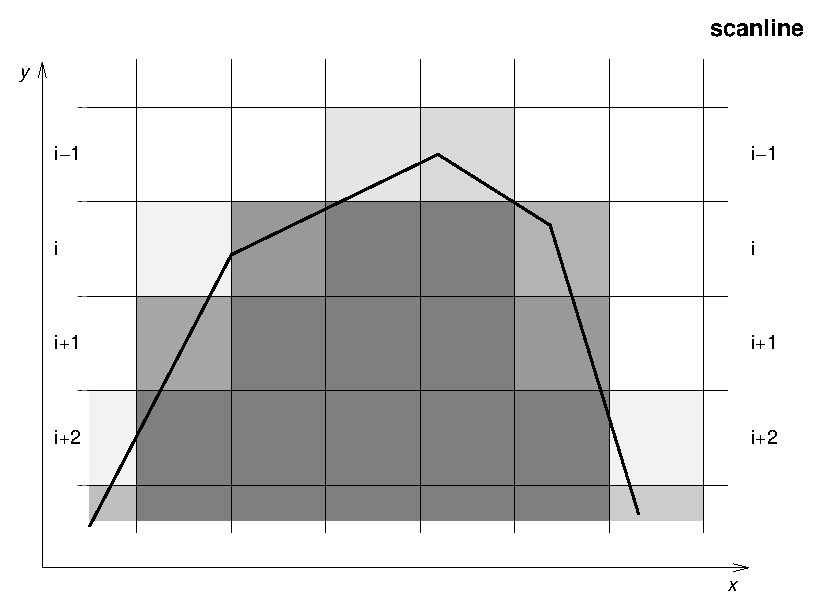
\includegraphics{scanline_n}\caption{scanline setup and alpha generation with antialiasing.}
\end{center}
\end{Image}


\subsection{Field Documentation}
\index{hpgs\_\-paint\_\-clipper\_\-st@{hpgs\_\-paint\_\-clipper\_\-st}!scanlines@{scanlines}}
\index{scanlines@{scanlines}!hpgs_paint_clipper_st@{hpgs\_\-paint\_\-clipper\_\-st}}
\subsubsection[scanlines]{\setlength{\rightskip}{0pt plus 5cm}{\bf hpgs\_\-paint\_\-scanline}$\ast$ {\bf hpgs\_\-paint\_\-clipper\_\-st::scanlines}}\label{structhpgs__paint__clipper__st_0bb91ce08576e1de31698acf4edb5a53}


The vector of scanlines in this clipper. 

Referenced by hpgs\_\-new\_\-paint\_\-clipper(), hpgs\_\-paint\_\-clipper\_\-clear(), hpgs\_\-paint\_\-clipper\_\-clip(), hpgs\_\-paint\_\-clipper\_\-destroy(), hpgs\_\-paint\_\-clipper\_\-emit(), hpgs\_\-paint\_\-clipper\_\-reset(), hpgs\_\-paint\_\-clipper\_\-thin\_\-cut(), and hpgs\_\-paint\_\-device\_\-drawimage().\index{hpgs\_\-paint\_\-clipper\_\-st@{hpgs\_\-paint\_\-clipper\_\-st}!yfac@{yfac}}
\index{yfac@{yfac}!hpgs_paint_clipper_st@{hpgs\_\-paint\_\-clipper\_\-st}}
\subsubsection[yfac]{\setlength{\rightskip}{0pt plus 5cm}double {\bf hpgs\_\-paint\_\-clipper\_\-st::yfac}}\label{structhpgs__paint__clipper__st_0cdd33a5c1f522e1445d74fd18ec2da2}


The bounding box of this clipper in world coordinates.

The mapping of scanline numbers to world coordinates. {\tt iscan=}(y0-y)/yfac and {\tt y=y0-iscan$\ast$yfac}. 

Referenced by hpgs\_\-new\_\-paint\_\-clipper(), and hpgs\_\-paint\_\-device\_\-drawimage().\index{hpgs\_\-paint\_\-clipper\_\-st@{hpgs\_\-paint\_\-clipper\_\-st}!overscan@{overscan}}
\index{overscan@{overscan}!hpgs_paint_clipper_st@{hpgs\_\-paint\_\-clipper\_\-st}}
\subsubsection[overscan]{\setlength{\rightskip}{0pt plus 5cm}hpgs\_\-bool {\bf hpgs\_\-paint\_\-clipper\_\-st::overscan}}\label{structhpgs__paint__clipper__st_b0fe1dce067b9c2fdbceb38bbe496e02}


Do we use antialiasing ?. 

Referenced by hpgs\_\-new\_\-paint\_\-clipper(), hpgs\_\-paint\_\-clipper\_\-clip(), hpgs\_\-paint\_\-clipper\_\-cut(), hpgs\_\-paint\_\-clipper\_\-emit(), and hpgs\_\-paint\_\-clipper\_\-reset().\index{hpgs\_\-paint\_\-clipper\_\-st@{hpgs\_\-paint\_\-clipper\_\-st}!height@{height}}
\index{height@{height}!hpgs_paint_clipper_st@{hpgs\_\-paint\_\-clipper\_\-st}}
\subsubsection[height]{\setlength{\rightskip}{0pt plus 5cm}int {\bf hpgs\_\-paint\_\-clipper\_\-st::height}}\label{structhpgs__paint__clipper__st_86d0fcb90e48b744eeb3ac6ffcb287ed}


Number of physical pixels of the underlying image. 

Referenced by hpgs\_\-new\_\-paint\_\-clipper(), hpgs\_\-paint\_\-clipper\_\-clip(), and hpgs\_\-paint\_\-clipper\_\-emit().\index{hpgs\_\-paint\_\-clipper\_\-st@{hpgs\_\-paint\_\-clipper\_\-st}!iscan0@{iscan0}}
\index{iscan0@{iscan0}!hpgs_paint_clipper_st@{hpgs\_\-paint\_\-clipper\_\-st}}
\subsubsection[iscan0]{\setlength{\rightskip}{0pt plus 5cm}int {\bf hpgs\_\-paint\_\-clipper\_\-st::iscan0}}\label{structhpgs__paint__clipper__st_23f85f972d3629d30f8f032640d4b77e}


The first scanline with non-zero intersections. 

Referenced by hpgs\_\-new\_\-paint\_\-clipper(), hpgs\_\-paint\_\-clipper\_\-clear(), hpgs\_\-paint\_\-clipper\_\-clip(), hpgs\_\-paint\_\-clipper\_\-emit(), hpgs\_\-paint\_\-clipper\_\-reset(), hpgs\_\-paint\_\-clipper\_\-thin\_\-cut(), and hpgs\_\-paint\_\-device\_\-drawimage().\index{hpgs\_\-paint\_\-clipper\_\-st@{hpgs\_\-paint\_\-clipper\_\-st}!iscan1@{iscan1}}
\index{iscan1@{iscan1}!hpgs_paint_clipper_st@{hpgs\_\-paint\_\-clipper\_\-st}}
\subsubsection[iscan1]{\setlength{\rightskip}{0pt plus 5cm}int {\bf hpgs\_\-paint\_\-clipper\_\-st::iscan1}}\label{structhpgs__paint__clipper__st_c2711333e8f5dfc95b6a33f0c4954b6f}


The last scanline with non-zero intersections. 

Referenced by hpgs\_\-new\_\-paint\_\-clipper(), hpgs\_\-paint\_\-clipper\_\-clear(), hpgs\_\-paint\_\-clipper\_\-clip(), hpgs\_\-paint\_\-clipper\_\-emit(), hpgs\_\-paint\_\-clipper\_\-reset(), and hpgs\_\-paint\_\-device\_\-drawimage().

The documentation for this struct was generated from the following file:\begin{CompactItemize}
\item 
{\bf hpgspaint.h}\end{CompactItemize}

\section{hpgs\_\-paint\_\-color\_\-st Struct Reference}
\label{structhpgs__paint__color__st}\index{hpgs\_\-paint\_\-color\_\-st@{hpgs\_\-paint\_\-color\_\-st}}
An image RGB color with an optional palette index.  


{\tt \#include $<$hpgs.h$>$}

\subsection*{Data Fields}
\begin{CompactItemize}
\item 
unsigned char \textbf{r}\label{structhpgs__paint__color__st_12daa9c92a80e567247c59451d8fe4f1}

\item 
unsigned char \textbf{g}\label{structhpgs__paint__color__st_def6a2ae2a146ecea42cfad60c276a9b}

\item 
unsigned char \textbf{b}\label{structhpgs__paint__color__st_154b2f2f04b37f774bc731d837161a27}

\item 
unsigned char \textbf{index}\label{structhpgs__paint__color__st_7335459b625a2c15af167e518eac9fe4}

\end{CompactItemize}


\subsection{Detailed Description}
An image RGB color with an optional palette index. 

This structure has a public alias {\tt hpgs\_\-paint\_\-color} and represents an image RGB color with an optional palette index consisting of single byte r,g and b color values in the range 0 to 255 as well as of a single byte palette index.

For calculating a suitable palette index for a given {\tt hpgs\_\-image} consider calling {\tt hpgs\_\-image\_\-define\_\-color}. 

The documentation for this struct was generated from the following file:\begin{CompactItemize}
\item 
{\bf hpgs.h}\end{CompactItemize}

\section{hpgs\_\-paint\_\-device\_\-st Struct Reference}
\label{structhpgs__paint__device__st}\index{hpgs\_\-paint\_\-device\_\-st@{hpgs\_\-paint\_\-device\_\-st}}
The pixel rendering vector graphics device.  


{\tt \#include $<$hpgspaint.h$>$}

\subsection*{Data Fields}
\begin{CompactItemize}
\item 
{\bf hpgs\_\-device} {\bf inherited}
\item 
{\bf hpgs\_\-image} $\ast$ {\bf image}
\item 
char $\ast$ {\bf filename}
\item 
{\bf hpgs\_\-bbox} \textbf{page\_\-bb}\label{structhpgs__paint__device__st_04170cbb3fbd8c6664587aafcbf897b3}

\item 
double {\bf xres}
\item 
double {\bf yres}
\item 
hpgs\_\-bool {\bf overscan}
\item 
double {\bf thin\_\-alpha}
\item 
{\bf hpgs\_\-paint\_\-path} $\ast$ {\bf path}
\item 
{\bf hpgs\_\-paint\_\-clipper} $\ast$ {\bf path\_\-clipper}
\item 
{\bf hpgs\_\-paint\_\-clipper} $\ast$ {\bf clippers} [HPGS\_\-PAINT\_\-MAX\_\-CLIP\_\-DEPTH]
\item 
int {\bf current\_\-clipper}
\item 
int {\bf clip\_\-depth}
\item 
{\bf hpgs\_\-gstate} $\ast$ {\bf gstate}
\item 
{\bf hpgs\_\-paint\_\-color} {\bf color}
\item 
{\bf hpgs\_\-palette\_\-color} {\bf patcol}
\item 
int {\bf image\_\-interpolation}
\end{CompactItemize}


\subsection{Detailed Description}
The pixel rendering vector graphics device. 

This structure has a public alias {\tt hpgs\_\-paint\_\-device} and represents a {\tt hpgs\_\-device} which draws to a given {\tt hpgs\_\-image}. It is capable of drawing polgonal data with optional antialiasing. Image may be drawn using a linear interpolation of the pixel values or uninterpolated.

The following figure outlines the coordinate setup of a paint device.

 \begin{Image}
\begin{center}
\includegraphics{clipper}\caption{Coordinate setup of hpgs\_\-paint\_\-device}
\end{center}
\end{Image}
 Further details on antialiasing and scanline setup are described in the documentation of {\tt \doxyref{hpgs\_\-paint\_\-clipper\_\-st}{p.}{structhpgs__paint__clipper__st}}. 

\subsection{Field Documentation}
\index{hpgs\_\-paint\_\-device\_\-st@{hpgs\_\-paint\_\-device\_\-st}!inherited@{inherited}}
\index{inherited@{inherited}!hpgs_paint_device_st@{hpgs\_\-paint\_\-device\_\-st}}
\subsubsection[inherited]{\setlength{\rightskip}{0pt plus 5cm}{\bf hpgs\_\-device} {\bf hpgs\_\-paint\_\-device\_\-st::inherited}}\label{structhpgs__paint__device__st_dce61d0854ddf04e4d9f3829b675c62c}


The base device structure. 

Referenced by hpgs\_\-new\_\-paint\_\-device().\index{hpgs\_\-paint\_\-device\_\-st@{hpgs\_\-paint\_\-device\_\-st}!image@{image}}
\index{image@{image}!hpgs_paint_device_st@{hpgs\_\-paint\_\-device\_\-st}}
\subsubsection[image]{\setlength{\rightskip}{0pt plus 5cm}{\bf hpgs\_\-image}$\ast$ {\bf hpgs\_\-paint\_\-device\_\-st::image}}\label{structhpgs__paint__device__st_84d585ae19d5bf9e2361533b887746dd}


The image to which we draw. 

Referenced by hpgs\_\-new\_\-paint\_\-device(), hpgs\_\-paint\_\-device\_\-drawimage(), and hpgs\_\-paint\_\-device\_\-fill().\index{hpgs\_\-paint\_\-device\_\-st@{hpgs\_\-paint\_\-device\_\-st}!filename@{filename}}
\index{filename@{filename}!hpgs_paint_device_st@{hpgs\_\-paint\_\-device\_\-st}}
\subsubsection[filename]{\setlength{\rightskip}{0pt plus 5cm}char$\ast$ {\bf hpgs\_\-paint\_\-device\_\-st::filename}}\label{structhpgs__paint__device__st_44bde06df9facc892568c83c6ecc2589}


The image filename without an eventual extension. 

Referenced by hpgs\_\-new\_\-paint\_\-device().\index{hpgs\_\-paint\_\-device\_\-st@{hpgs\_\-paint\_\-device\_\-st}!xres@{xres}}
\index{xres@{xres}!hpgs_paint_device_st@{hpgs\_\-paint\_\-device\_\-st}}
\subsubsection[xres]{\setlength{\rightskip}{0pt plus 5cm}double {\bf hpgs\_\-paint\_\-device\_\-st::xres}}\label{structhpgs__paint__device__st_a93dd6cdbfad32c8b5cf5d1e8d2a85d5}


The bounding box in world coordinates, which is mapped onto the image. The resolution of the image in x direction. 

Referenced by hpgs\_\-new\_\-paint\_\-device().\index{hpgs\_\-paint\_\-device\_\-st@{hpgs\_\-paint\_\-device\_\-st}!yres@{yres}}
\index{yres@{yres}!hpgs_paint_device_st@{hpgs\_\-paint\_\-device\_\-st}}
\subsubsection[yres]{\setlength{\rightskip}{0pt plus 5cm}double {\bf hpgs\_\-paint\_\-device\_\-st::yres}}\label{structhpgs__paint__device__st_cc5bcb2f4ff2e9ae558a59bf70588f7b}


The resolution of the image in y direction. 

Referenced by hpgs\_\-new\_\-paint\_\-device().\index{hpgs\_\-paint\_\-device\_\-st@{hpgs\_\-paint\_\-device\_\-st}!overscan@{overscan}}
\index{overscan@{overscan}!hpgs_paint_device_st@{hpgs\_\-paint\_\-device\_\-st}}
\subsubsection[overscan]{\setlength{\rightskip}{0pt plus 5cm}hpgs\_\-bool {\bf hpgs\_\-paint\_\-device\_\-st::overscan}}\label{structhpgs__paint__device__st_233bef1702634fd2639856ba39c50794}


Specifies, whether we use antialiasing for rendering the image. 

Referenced by hpgs\_\-new\_\-paint\_\-device(), and hpgs\_\-paint\_\-device\_\-drawimage().\index{hpgs\_\-paint\_\-device\_\-st@{hpgs\_\-paint\_\-device\_\-st}!thin\_\-alpha@{thin\_\-alpha}}
\index{thin\_\-alpha@{thin\_\-alpha}!hpgs_paint_device_st@{hpgs\_\-paint\_\-device\_\-st}}
\subsubsection[thin\_\-alpha]{\setlength{\rightskip}{0pt plus 5cm}double {\bf hpgs\_\-paint\_\-device\_\-st::thin\_\-alpha}}\label{structhpgs__paint__device__st_f969769ac0f47742723bfe31f17ea3e1}


The minimal alpha value for antialiased thin lines. 

Referenced by hpgs\_\-new\_\-paint\_\-device(), and hpgs\_\-paint\_\-device\_\-set\_\-thin\_\-alpha().\index{hpgs\_\-paint\_\-device\_\-st@{hpgs\_\-paint\_\-device\_\-st}!path@{path}}
\index{path@{path}!hpgs_paint_device_st@{hpgs\_\-paint\_\-device\_\-st}}
\subsubsection[path]{\setlength{\rightskip}{0pt plus 5cm}{\bf hpgs\_\-paint\_\-path}$\ast$ {\bf hpgs\_\-paint\_\-device\_\-st::path}}\label{structhpgs__paint__device__st_474f2a7513da961e63a256b8d54b369f}


The current path, which is under contruction. 

Referenced by hpgs\_\-new\_\-paint\_\-device().\index{hpgs\_\-paint\_\-device\_\-st@{hpgs\_\-paint\_\-device\_\-st}!path\_\-clipper@{path\_\-clipper}}
\index{path\_\-clipper@{path\_\-clipper}!hpgs_paint_device_st@{hpgs\_\-paint\_\-device\_\-st}}
\subsubsection[path\_\-clipper]{\setlength{\rightskip}{0pt plus 5cm}{\bf hpgs\_\-paint\_\-clipper}$\ast$ {\bf hpgs\_\-paint\_\-device\_\-st::path\_\-clipper}}\label{structhpgs__paint__device__st_e85a15e0017fe8fe7d4d70febd262143}


The mapping of the current path onto the defined scanlines. 

Referenced by hpgs\_\-new\_\-paint\_\-device(), hpgs\_\-paint\_\-device\_\-clip(), and hpgs\_\-paint\_\-device\_\-fill().\index{hpgs\_\-paint\_\-device\_\-st@{hpgs\_\-paint\_\-device\_\-st}!clippers@{clippers}}
\index{clippers@{clippers}!hpgs_paint_device_st@{hpgs\_\-paint\_\-device\_\-st}}
\subsubsection[clippers]{\setlength{\rightskip}{0pt plus 5cm}{\bf hpgs\_\-paint\_\-clipper}$\ast$ {\bf hpgs\_\-paint\_\-device\_\-st::clippers}[HPGS\_\-PAINT\_\-MAX\_\-CLIP\_\-DEPTH]}\label{structhpgs__paint__device__st_a98e8324dee571ed20f107483847e366}


A stack of mappings of the clip path' of onto the defined scanlines. 

Referenced by hpgs\_\-new\_\-paint\_\-device(), hpgs\_\-paint\_\-device\_\-clip(), hpgs\_\-paint\_\-device\_\-drawimage(), and hpgs\_\-paint\_\-device\_\-fill().\index{hpgs\_\-paint\_\-device\_\-st@{hpgs\_\-paint\_\-device\_\-st}!current\_\-clipper@{current\_\-clipper}}
\index{current\_\-clipper@{current\_\-clipper}!hpgs_paint_device_st@{hpgs\_\-paint\_\-device\_\-st}}
\subsubsection[current\_\-clipper]{\setlength{\rightskip}{0pt plus 5cm}int {\bf hpgs\_\-paint\_\-device\_\-st::current\_\-clipper}}\label{structhpgs__paint__device__st_f3cd0db225d18d3195dbf86942f17e0a}


The position of the current clip path in {\tt clippers}. 

Referenced by hpgs\_\-new\_\-paint\_\-device(), hpgs\_\-paint\_\-device\_\-clip(), hpgs\_\-paint\_\-device\_\-drawimage(), and hpgs\_\-paint\_\-device\_\-fill().\index{hpgs\_\-paint\_\-device\_\-st@{hpgs\_\-paint\_\-device\_\-st}!clip\_\-depth@{clip\_\-depth}}
\index{clip\_\-depth@{clip\_\-depth}!hpgs_paint_device_st@{hpgs\_\-paint\_\-device\_\-st}}
\subsubsection[clip\_\-depth]{\setlength{\rightskip}{0pt plus 5cm}int {\bf hpgs\_\-paint\_\-device\_\-st::clip\_\-depth}}\label{structhpgs__paint__device__st_9ecd7529554b6249290b533218539ad6}


The current depth of the clip stack, i.e. the number of time {\tt hpgs\_\-clip} or {\tt hpgs\_\-eoclip} has been called. 

Referenced by hpgs\_\-new\_\-paint\_\-device(), and hpgs\_\-paint\_\-device\_\-clip().\index{hpgs\_\-paint\_\-device\_\-st@{hpgs\_\-paint\_\-device\_\-st}!gstate@{gstate}}
\index{gstate@{gstate}!hpgs_paint_device_st@{hpgs\_\-paint\_\-device\_\-st}}
\subsubsection[gstate]{\setlength{\rightskip}{0pt plus 5cm}{\bf hpgs\_\-gstate}$\ast$ {\bf hpgs\_\-paint\_\-device\_\-st::gstate}}\label{structhpgs__paint__device__st_35c2a8bdca8f5af3647b3f467f6c18fc}


The graphics state. 

Referenced by hpgs\_\-new\_\-paint\_\-device().\index{hpgs\_\-paint\_\-device\_\-st@{hpgs\_\-paint\_\-device\_\-st}!color@{color}}
\index{color@{color}!hpgs_paint_device_st@{hpgs\_\-paint\_\-device\_\-st}}
\subsubsection[color]{\setlength{\rightskip}{0pt plus 5cm}{\bf hpgs\_\-paint\_\-color} {\bf hpgs\_\-paint\_\-device\_\-st::color}}\label{structhpgs__paint__device__st_4416f203bdb3593dd972ef27a44e8f68}


The current color transformed to a device color. 

Referenced by hpgs\_\-new\_\-paint\_\-device(), and hpgs\_\-paint\_\-device\_\-fill().\index{hpgs\_\-paint\_\-device\_\-st@{hpgs\_\-paint\_\-device\_\-st}!patcol@{patcol}}
\index{patcol@{patcol}!hpgs_paint_device_st@{hpgs\_\-paint\_\-device\_\-st}}
\subsubsection[patcol]{\setlength{\rightskip}{0pt plus 5cm}{\bf hpgs\_\-palette\_\-color} {\bf hpgs\_\-paint\_\-device\_\-st::patcol}}\label{structhpgs__paint__device__st_cf74cf935da979569aa6774d55e9cb10}


The current pattern color transformed to a device color. 

Referenced by hpgs\_\-new\_\-paint\_\-device().\index{hpgs\_\-paint\_\-device\_\-st@{hpgs\_\-paint\_\-device\_\-st}!image\_\-interpolation@{image\_\-interpolation}}
\index{image\_\-interpolation@{image\_\-interpolation}!hpgs_paint_device_st@{hpgs\_\-paint\_\-device\_\-st}}
\subsubsection[image\_\-interpolation]{\setlength{\rightskip}{0pt plus 5cm}int {\bf hpgs\_\-paint\_\-device\_\-st::image\_\-interpolation}}\label{structhpgs__paint__device__st_b0bf0ff09e650c45c9d3d6d9db182fd6}


A flag holding whether we do image interpolation. 

Referenced by hpgs\_\-new\_\-paint\_\-device(), hpgs\_\-paint\_\-device\_\-drawimage(), and hpgs\_\-paint\_\-device\_\-set\_\-image\_\-interpolation().

The documentation for this struct was generated from the following file:\begin{CompactItemize}
\item 
{\bf hpgspaint.h}\end{CompactItemize}

\section{hpgs\_\-paint\_\-path\_\-st Struct Reference}
\label{structhpgs__paint__path__st}\index{hpgs\_\-paint\_\-path\_\-st@{hpgs\_\-paint\_\-path\_\-st}}
A stored vector path.  


{\tt \#include $<$hpgs.h$>$}

\subsection*{Data Fields}
\begin{CompactItemize}
\item 
{\bf hpgs\_\-bbox} \textbf{bb}\label{structhpgs__paint__path__st_f4ae3fb2b6fd1725377c0399b8506b23}

\end{CompactItemize}
\begin{Indent}{\bf }\par
\begin{CompactItemize}
\item 
{\bf hpgs\_\-path\_\-point} $\ast$ {\bf points}
\item 
int \textbf{n\_\-points}\label{structhpgs__paint__path__st_3180496eb7ad6dd7bd9a84a6393f9ea9}

\item 
int \textbf{last\_\-start}\label{structhpgs__paint__path__st_b74ad95c8195e77194d3a79191823be0}

\item 
int \textbf{points\_\-malloc\_\-size}\label{structhpgs__paint__path__st_d251d2fedecc7e918c83cfd05d4fb358}

\end{CompactItemize}
\end{Indent}


\subsection{Detailed Description}
A stored vector path. 

This structure has a public alias {\tt hpgs\_\-paint\_\-path} and represents a polygonal path, which is stores the path topology together with cached informations about bezier splines. 

\subsection{Field Documentation}
\index{hpgs\_\-paint\_\-path\_\-st@{hpgs\_\-paint\_\-path\_\-st}!points@{points}}
\index{points@{points}!hpgs_paint_path_st@{hpgs\_\-paint\_\-path\_\-st}}
\subsubsection[points]{\setlength{\rightskip}{0pt plus 5cm}{\bf hpgs\_\-path\_\-point}$\ast$ {\bf hpgs\_\-paint\_\-path\_\-st::points}}\label{structhpgs__paint__path__st_8731bebc1e5715a5e4838035349afc3e}


A stack of path points. {\tt last\_\-start} indicates the index of the last start of a subpolygon. This is information is needed during path construction. 

Referenced by hpgs\_\-bezier\_\-path\_\-delta(), hpgs\_\-bezier\_\-path\_\-delta\_\-x(), hpgs\_\-bezier\_\-path\_\-delta\_\-y(), hpgs\_\-bezier\_\-path\_\-point(), hpgs\_\-bezier\_\-path\_\-singularities(), hpgs\_\-bezier\_\-path\_\-to\_\-quadratic(), hpgs\_\-bezier\_\-path\_\-x(), hpgs\_\-bezier\_\-path\_\-xmax(), hpgs\_\-bezier\_\-path\_\-xmin(), hpgs\_\-bezier\_\-path\_\-y(), hpgs\_\-bezier\_\-path\_\-ymax(), hpgs\_\-bezier\_\-path\_\-ymin(), hpgs\_\-new\_\-paint\_\-path(), hpgs\_\-paint\_\-path\_\-buldgeto(), hpgs\_\-paint\_\-path\_\-closepath(), hpgs\_\-paint\_\-path\_\-curveto(), hpgs\_\-paint\_\-path\_\-destroy(), hpgs\_\-paint\_\-path\_\-lineto(), and hpgs\_\-paint\_\-path\_\-moveto().

The documentation for this struct was generated from the following file:\begin{CompactItemize}
\item 
{\bf hpgs.h}\end{CompactItemize}

\section{hpgs\_\-paint\_\-scanline\_\-st Struct Reference}
\label{structhpgs__paint__scanline__st}\index{hpgs\_\-paint\_\-scanline\_\-st@{hpgs\_\-paint\_\-scanline\_\-st}}
A scanline of the pixel renderer.  


{\tt \#include $<$hpgspaint.h$>$}

\subsection*{Data Fields}
\begin{Indent}{\bf }\par
\begin{CompactItemize}
\item 
{\bf hpgs\_\-scanline\_\-point} $\ast$ {\bf points}
\item 
int \textbf{points\_\-malloc\_\-size}\label{structhpgs__paint__scanline__st_19a51f9f8896740a26bb07ef277500c0}

\item 
int \textbf{n\_\-points}\label{structhpgs__paint__scanline__st_2e5ba769139b867a4bd641c34a91b75e}

\end{CompactItemize}
\end{Indent}


\subsection{Detailed Description}
A scanline of the pixel renderer. 

This structure has a public alias {\tt hpgs\_\-paint\_\-scanline} and holds the intersections points of a path with a scanline. 

\subsection{Field Documentation}
\index{hpgs\_\-paint\_\-scanline\_\-st@{hpgs\_\-paint\_\-scanline\_\-st}!points@{points}}
\index{points@{points}!hpgs_paint_scanline_st@{hpgs\_\-paint\_\-scanline\_\-st}}
\subsubsection[points]{\setlength{\rightskip}{0pt plus 5cm}{\bf hpgs\_\-scanline\_\-point}$\ast$ {\bf hpgs\_\-paint\_\-scanline\_\-st::points}}\label{structhpgs__paint__scanline__st_596e27a603eeeb05fafa0215ed518898}


A vector of intersection points. 

Referenced by hpgs\_\-paint\_\-clipper\_\-thin\_\-cut(), and hpgs\_\-paint\_\-device\_\-drawimage().

The documentation for this struct was generated from the following file:\begin{CompactItemize}
\item 
{\bf hpgspaint.h}\end{CompactItemize}

\section{hpgs\_\-palette\_\-color\_\-st Struct Reference}
\label{structhpgs__palette__color__st}\index{hpgs\_\-palette\_\-color\_\-st@{hpgs\_\-palette\_\-color\_\-st}}
A screen RGB color as stored in a palette.  


{\tt \#include $<$hpgs.h$>$}

\subsection*{Data Fields}
\begin{CompactItemize}
\item 
unsigned char \textbf{r}\label{structhpgs__palette__color__st_4c1c1cc206462ddf3859578221011dbb}

\item 
unsigned char \textbf{g}\label{structhpgs__palette__color__st_7c7f8e4b90a61257de498677d0441f60}

\item 
unsigned char \textbf{b}\label{structhpgs__palette__color__st_05b25a11373ddb61f6102fdb8ba4ba37}

\end{CompactItemize}


\subsection{Detailed Description}
A screen RGB color as stored in a palette. 

This structure has a public alias {\tt hpgs\_\-palette\_\-color} and represents a screen RGB color consisting of single byte r,g and b color values in the range 0 to 255. 

The documentation for this struct was generated from the following file:\begin{CompactItemize}
\item 
{\bf hpgs.h}\end{CompactItemize}

\section{hpgs\_\-path\_\-point\_\-st Struct Reference}
\label{structhpgs__path__point__st}\index{hpgs\_\-path\_\-point\_\-st@{hpgs\_\-path\_\-point\_\-st}}
A point in a stored path.  


{\tt \#include $<$hpgs.h$>$}

\subsection*{Data Fields}
\begin{CompactItemize}
\item 
{\bf hpgs\_\-point} {\bf p}
\item 
int {\bf flags}
\end{CompactItemize}


\subsection{Detailed Description}
A point in a stored path. 

This structure has a public alias {\tt hpgs\_\-path\_\-point} and represents a point of a polygonal path. 

\subsection{Field Documentation}
\index{hpgs\_\-path\_\-point\_\-st@{hpgs\_\-path\_\-point\_\-st}!p@{p}}
\index{p@{p}!hpgs_path_point_st@{hpgs\_\-path\_\-point\_\-st}}
\subsubsection[p]{\setlength{\rightskip}{0pt plus 5cm}{\bf hpgs\_\-point} {\bf hpgs\_\-path\_\-point\_\-st::p}}\label{structhpgs__path__point__st_c89eeb90383204d79e177f60f99c5f5e}


Coordinates of this path point. 

Referenced by hpgs\_\-bezier\_\-path\_\-delta(), hpgs\_\-bezier\_\-path\_\-delta\_\-x(), hpgs\_\-bezier\_\-path\_\-delta\_\-y(), hpgs\_\-bezier\_\-path\_\-point(), hpgs\_\-bezier\_\-path\_\-singularities(), hpgs\_\-bezier\_\-path\_\-to\_\-quadratic(), hpgs\_\-bezier\_\-path\_\-x(), hpgs\_\-bezier\_\-path\_\-xmax(), hpgs\_\-bezier\_\-path\_\-xmin(), hpgs\_\-bezier\_\-path\_\-y(), hpgs\_\-bezier\_\-path\_\-ymax(), hpgs\_\-bezier\_\-path\_\-ymin(), hpgs\_\-paint\_\-path\_\-buldgeto(), hpgs\_\-paint\_\-path\_\-closepath(), hpgs\_\-paint\_\-path\_\-lineto(), and hpgs\_\-paint\_\-path\_\-moveto().\index{hpgs\_\-path\_\-point\_\-st@{hpgs\_\-path\_\-point\_\-st}!flags@{flags}}
\index{flags@{flags}!hpgs_path_point_st@{hpgs\_\-path\_\-point\_\-st}}
\subsubsection[flags]{\setlength{\rightskip}{0pt plus 5cm}int {\bf hpgs\_\-path\_\-point\_\-st::flags}}\label{structhpgs__path__point__st_1a077ee4742f3a52cc403e82b997a1bc}


Flags for this path point. 

Referenced by hpgs\_\-paint\_\-path\_\-closepath(), hpgs\_\-paint\_\-path\_\-curveto(), hpgs\_\-paint\_\-path\_\-lineto(), and hpgs\_\-paint\_\-path\_\-moveto().

The documentation for this struct was generated from the following file:\begin{CompactItemize}
\item 
{\bf hpgs.h}\end{CompactItemize}

\section{hpgs\_\-plotsize\_\-device\_\-st Struct Reference}
\label{structhpgs__plotsize__device__st}\index{hpgs\_\-plotsize\_\-device\_\-st@{hpgs\_\-plotsize\_\-device\_\-st}}
A vector graphics device for plotsize calculating.  


{\tt \#include $<$hpgsdevices.h$>$}

\subsection*{Data Fields}
\begin{CompactItemize}
\item 
{\bf hpgs\_\-device} {\bf inherited}\label{structhpgs__plotsize__device__st_896e5ef39be8fb94f861db9d51800c3e}

\begin{CompactList}\small\item\em The base device structure. \item\end{CompactList}\item 
hpgs\_\-bool {\bf ignore\_\-ps}\label{structhpgs__plotsize__device__st_b33cc0245c082105f5bb0cb9a1ce47b2}

\begin{CompactList}\small\item\em Do we ignore a PS command? \item\end{CompactList}\item 
int {\bf clip\_\-depth}\label{structhpgs__plotsize__device__st_397e61533c894d3396d6452572cecaf3}

\begin{CompactList}\small\item\em The depth of the current clip path stack. \item\end{CompactList}\item 
{\bf hpgs\_\-point} {\bf moveto}\label{structhpgs__plotsize__device__st_69ad990dc8df48bde3470d1dd562beac}

\begin{CompactList}\small\item\em The position of the last moveto. \item\end{CompactList}\item 
int {\bf deferred\_\-moveto}\label{structhpgs__plotsize__device__st_5322a4a685eb24f0a3ef5bf897a85364}

\begin{CompactList}\small\item\em Do we have an unregistered moveto pending? \item\end{CompactList}\item 
hpgs\_\-bool {\bf do\_\-linewidth}\label{structhpgs__plotsize__device__st_e8e92266b09da342dbd1f1cc26dd914d}

\begin{CompactList}\small\item\em Do we account for the current linewidth? \item\end{CompactList}\item 
double {\bf linewidth}\label{structhpgs__plotsize__device__st_e18ef2c36ee97539c25b88dd1cbf4368}

\begin{CompactList}\small\item\em Current linewidth. \item\end{CompactList}\item 
{\bf hpgs\_\-bbox} \textbf{clip\_\-bbs} [HPGS\_\-PLOTSIZE\_\-MAX\_\-CLIP\_\-DEPTH]\label{structhpgs__plotsize__device__st_ce813b5e80f82a23bfd48844c21bc67f}

\item 
{\bf hpgs\_\-bbox} {\bf path\_\-bb}
\item 
{\bf hpgs\_\-bbox} {\bf page\_\-bb}
\item 
{\bf hpgs\_\-bbox} {\bf global\_\-bb}
\end{CompactItemize}
\begin{Indent}{\bf }\par
\begin{CompactItemize}
\item 
{\bf hpgs\_\-bbox} $\ast$ {\bf page\_\-bbs}
\item 
int {\bf n\_\-page\_\-bbs}
\item 
int \textbf{page\_\-bbs\_\-alloc\_\-size}\label{structhpgs__plotsize__device__st_0d0a3522e149fdd32062286a75316d4a}

\end{CompactItemize}
\end{Indent}


\subsection{Detailed Description}
A vector graphics device for plotsize calculating. 

This structure implements a {\tt hpgs\_\-device} and is used to calculate the bounding box of a vector graphics scenery. 

\subsection{Field Documentation}
\index{hpgs\_\-plotsize\_\-device\_\-st@{hpgs\_\-plotsize\_\-device\_\-st}!path\_\-bb@{path\_\-bb}}
\index{path\_\-bb@{path\_\-bb}!hpgs_plotsize_device_st@{hpgs\_\-plotsize\_\-device\_\-st}}
\subsubsection[path\_\-bb]{\setlength{\rightskip}{0pt plus 5cm}{\bf hpgs\_\-bbox} {\bf hpgs\_\-plotsize\_\-device\_\-st::path\_\-bb}}\label{structhpgs__plotsize__device__st_35db4a71c68d2dadd16f2fe5628af408}


The bounding boxes of the clip paths. 

Referenced by hpgs\_\-new\_\-plotsize\_\-device().\index{hpgs\_\-plotsize\_\-device\_\-st@{hpgs\_\-plotsize\_\-device\_\-st}!page\_\-bb@{page\_\-bb}}
\index{page\_\-bb@{page\_\-bb}!hpgs_plotsize_device_st@{hpgs\_\-plotsize\_\-device\_\-st}}
\subsubsection[page\_\-bb]{\setlength{\rightskip}{0pt plus 5cm}{\bf hpgs\_\-bbox} {\bf hpgs\_\-plotsize\_\-device\_\-st::page\_\-bb}}\label{structhpgs__plotsize__device__st_1facd325cac492ed0f0e4ceae0e51b61}


The bounding box of the current path. 

Referenced by hpgs\_\-new\_\-plotsize\_\-device().\index{hpgs\_\-plotsize\_\-device\_\-st@{hpgs\_\-plotsize\_\-device\_\-st}!global\_\-bb@{global\_\-bb}}
\index{global\_\-bb@{global\_\-bb}!hpgs_plotsize_device_st@{hpgs\_\-plotsize\_\-device\_\-st}}
\subsubsection[global\_\-bb]{\setlength{\rightskip}{0pt plus 5cm}{\bf hpgs\_\-bbox} {\bf hpgs\_\-plotsize\_\-device\_\-st::global\_\-bb}}\label{structhpgs__plotsize__device__st_ff4e09e9145c2584b76ba475bdbe7925}


The bounding box of the current page. 

Referenced by hpgs\_\-new\_\-plotsize\_\-device().\index{hpgs\_\-plotsize\_\-device\_\-st@{hpgs\_\-plotsize\_\-device\_\-st}!page\_\-bbs@{page\_\-bbs}}
\index{page\_\-bbs@{page\_\-bbs}!hpgs_plotsize_device_st@{hpgs\_\-plotsize\_\-device\_\-st}}
\subsubsection[page\_\-bbs]{\setlength{\rightskip}{0pt plus 5cm}{\bf hpgs\_\-bbox}$\ast$ {\bf hpgs\_\-plotsize\_\-device\_\-st::page\_\-bbs}}\label{structhpgs__plotsize__device__st_016fbde7815a9034098f94cb60e0dcdd}


The currently calculated overall bounding box.

A stack of page bounding boxes. 

Referenced by hpgs\_\-new\_\-plotsize\_\-device().\index{hpgs\_\-plotsize\_\-device\_\-st@{hpgs\_\-plotsize\_\-device\_\-st}!n\_\-page\_\-bbs@{n\_\-page\_\-bbs}}
\index{n\_\-page\_\-bbs@{n\_\-page\_\-bbs}!hpgs_plotsize_device_st@{hpgs\_\-plotsize\_\-device\_\-st}}
\subsubsection[n\_\-page\_\-bbs]{\setlength{\rightskip}{0pt plus 5cm}int {\bf hpgs\_\-plotsize\_\-device\_\-st::n\_\-page\_\-bbs}}\label{structhpgs__plotsize__device__st_9375b4471761001e8a68d70e62612f0d}


The currently calculated overall bounding box. 

Referenced by hpgs\_\-new\_\-plotsize\_\-device().

The documentation for this struct was generated from the following file:\begin{CompactItemize}
\item 
{\bf hpgsdevices.h}\end{CompactItemize}

\section{hpgs\_\-point\_\-st Struct Reference}
\label{structhpgs__point__st}\index{hpgs\_\-point\_\-st@{hpgs\_\-point\_\-st}}
A 2D point.  


{\tt \#include $<$hpgs.h$>$}

\subsection*{Data Fields}
\begin{CompactItemize}
\item 
double \textbf{x}\label{structhpgs__point__st_511eb8c19d4db5d0de9056d168cda20f}

\item 
double \textbf{y}\label{structhpgs__point__st_635076d8d6573e32f3ae6d2222807ed0}

\end{CompactItemize}


\subsection{Detailed Description}
A 2D point. 

This structure has a public alias {\tt hpgs\_\-point} and represents a point consisting of double precision x and y coordinates. 

The documentation for this struct was generated from the following file:\begin{CompactItemize}
\item 
{\bf hpgs.h}\end{CompactItemize}

\section{hpgs\_\-ps\_\-media\_\-size\_\-st Struct Reference}
\label{structhpgs__ps__media__size__st}\index{hpgs\_\-ps\_\-media\_\-size\_\-st@{hpgs\_\-ps\_\-media\_\-size\_\-st}}
A structure for storing a paper size.  


{\tt \#include $<$hpgsdevices.h$>$}

\subsection*{Data Fields}
\begin{CompactItemize}
\item 
int {\bf width}\label{structhpgs__ps__media__size__st_ca91814a4af3989fb51c2e58c51e523a}

\begin{CompactList}\small\item\em The width of the paper in pt. \item\end{CompactList}\item 
int {\bf height}\label{structhpgs__ps__media__size__st_106d89beb31eb46aa807ef2c3302bc95}

\begin{CompactList}\small\item\em The height of the paper in pt. \item\end{CompactList}\item 
const char $\ast$ {\bf name}\label{structhpgs__ps__media__size__st_3384834f44a02e470913195e64e93d5a}

\begin{CompactList}\small\item\em The name of this paper size, if it is a std paper size. \item\end{CompactList}\item 
size\_\-t {\bf usage}\label{structhpgs__ps__media__size__st_cea1bedaf8494023dc288edd3e7f5fbf}

\begin{CompactList}\small\item\em The usage count of this paper size. \item\end{CompactList}\item 
size\_\-t {\bf hash}\label{structhpgs__ps__media__size__st_5b695a806ae47a840a649170860754b6}

\begin{CompactList}\small\item\em A hash value for storing media sizes in a sorted vector. \item\end{CompactList}\end{CompactItemize}


\subsection{Detailed Description}
A structure for storing a paper size. 

This structure stores a PostScipt paper size. 

The documentation for this struct was generated from the following file:\begin{CompactItemize}
\item 
{\bf hpgsdevices.h}\end{CompactItemize}

\section{hpgs\_\-reader\_\-pcl\_\-palette\_\-st Struct Reference}
\label{structhpgs__reader__pcl__palette__st}\index{hpgs\_\-reader\_\-pcl\_\-palette\_\-st@{hpgs\_\-reader\_\-pcl\_\-palette\_\-st}}
A PCL palette as used by PCL push/pop palette.  


{\tt \#include $<$hpgsreader.h$>$}

\subsection*{Data Fields}
\begin{CompactItemize}
\item 
{\bf hpgs\_\-palette\_\-color} {\bf colors} [256]
\item 
{\bf hpgs\_\-palette\_\-color} {\bf last\_\-color}
\item 
int {\bf cid\_\-space}
\item 
int {\bf cid\_\-enc}
\item 
int {\bf cid\_\-bpi}
\item 
int {\bf cid\_\-bpc} [3]
\end{CompactItemize}


\subsection{Detailed Description}
A PCL palette as used by PCL push/pop palette. 

This structure holds all properties which are saved/resoterd through PCL push/pop palette. 

\subsection{Field Documentation}
\index{hpgs\_\-reader\_\-pcl\_\-palette\_\-st@{hpgs\_\-reader\_\-pcl\_\-palette\_\-st}!colors@{colors}}
\index{colors@{colors}!hpgs_reader_pcl_palette_st@{hpgs\_\-reader\_\-pcl\_\-palette\_\-st}}
\subsubsection[colors]{\setlength{\rightskip}{0pt plus 5cm}{\bf hpgs\_\-palette\_\-color} {\bf hpgs\_\-reader\_\-pcl\_\-palette\_\-st::colors}[256]}\label{structhpgs__reader__pcl__palette__st_4efdd1a3a0373c21a1c98b64033f15d9}


The palette colors. \index{hpgs\_\-reader\_\-pcl\_\-palette\_\-st@{hpgs\_\-reader\_\-pcl\_\-palette\_\-st}!last\_\-color@{last\_\-color}}
\index{last\_\-color@{last\_\-color}!hpgs_reader_pcl_palette_st@{hpgs\_\-reader\_\-pcl\_\-palette\_\-st}}
\subsubsection[last\_\-color]{\setlength{\rightskip}{0pt plus 5cm}{\bf hpgs\_\-palette\_\-color} {\bf hpgs\_\-reader\_\-pcl\_\-palette\_\-st::last\_\-color}}\label{structhpgs__reader__pcl__palette__st_50da3dcb4c2daf88010b738911974067}


The PCL color currently being assembled. \index{hpgs\_\-reader\_\-pcl\_\-palette\_\-st@{hpgs\_\-reader\_\-pcl\_\-palette\_\-st}!cid\_\-space@{cid\_\-space}}
\index{cid\_\-space@{cid\_\-space}!hpgs_reader_pcl_palette_st@{hpgs\_\-reader\_\-pcl\_\-palette\_\-st}}
\subsubsection[cid\_\-space]{\setlength{\rightskip}{0pt plus 5cm}int {\bf hpgs\_\-reader\_\-pcl\_\-palette\_\-st::cid\_\-space}}\label{structhpgs__reader__pcl__palette__st_ce3db697f9516fac5a49520703121254}


The current PCL color space. \index{hpgs\_\-reader\_\-pcl\_\-palette\_\-st@{hpgs\_\-reader\_\-pcl\_\-palette\_\-st}!cid\_\-enc@{cid\_\-enc}}
\index{cid\_\-enc@{cid\_\-enc}!hpgs_reader_pcl_palette_st@{hpgs\_\-reader\_\-pcl\_\-palette\_\-st}}
\subsubsection[cid\_\-enc]{\setlength{\rightskip}{0pt plus 5cm}int {\bf hpgs\_\-reader\_\-pcl\_\-palette\_\-st::cid\_\-enc}}\label{structhpgs__reader__pcl__palette__st_e5087fbe950254566bfabdd670d727d8}


The current PCL pixel encoding scheme. \index{hpgs\_\-reader\_\-pcl\_\-palette\_\-st@{hpgs\_\-reader\_\-pcl\_\-palette\_\-st}!cid\_\-bpi@{cid\_\-bpi}}
\index{cid\_\-bpi@{cid\_\-bpi}!hpgs_reader_pcl_palette_st@{hpgs\_\-reader\_\-pcl\_\-palette\_\-st}}
\subsubsection[cid\_\-bpi]{\setlength{\rightskip}{0pt plus 5cm}int {\bf hpgs\_\-reader\_\-pcl\_\-palette\_\-st::cid\_\-bpi}}\label{structhpgs__reader__pcl__palette__st_fcf9de2306283e738215d312455cc222}


PCL Bits per color index. \index{hpgs\_\-reader\_\-pcl\_\-palette\_\-st@{hpgs\_\-reader\_\-pcl\_\-palette\_\-st}!cid\_\-bpc@{cid\_\-bpc}}
\index{cid\_\-bpc@{cid\_\-bpc}!hpgs_reader_pcl_palette_st@{hpgs\_\-reader\_\-pcl\_\-palette\_\-st}}
\subsubsection[cid\_\-bpc]{\setlength{\rightskip}{0pt plus 5cm}int {\bf hpgs\_\-reader\_\-pcl\_\-palette\_\-st::cid\_\-bpc}[3]}\label{structhpgs__reader__pcl__palette__st_7fcff7f264204990c01632d0a603d6e2}


PCL Bits per color component. 

The documentation for this struct was generated from the following file:\begin{CompactItemize}
\item 
{\bf hpgsreader.h}\end{CompactItemize}

\section{hpgs\_\-reader\_\-poly\_\-point\_\-st Struct Reference}
\label{structhpgs__reader__poly__point__st}\index{hpgs\_\-reader\_\-poly\_\-point\_\-st@{hpgs\_\-reader\_\-poly\_\-point\_\-st}}
A point in hte HPGL polygon buffer.  


{\tt \#include $<$hpgsreader.h$>$}

\subsection*{Data Fields}
\begin{CompactItemize}
\item 
{\bf hpgs\_\-point} {\bf p}\label{structhpgs__reader__poly__point__st_43e696e9d5d92fa2008401d433a89345}

\begin{CompactList}\small\item\em The coordinates of the point. \item\end{CompactList}\item 
int {\bf flag}\label{structhpgs__reader__poly__point__st_f1d9dc9590231f824b5b424dccbf89c1}

\begin{CompactList}\small\item\em 0 moveto, 1 lineto, 2 curveto \item\end{CompactList}\end{CompactItemize}


\subsection{Detailed Description}
A point in hte HPGL polygon buffer. 

This structure holds a point in the polygon buffer of HPGL used to implement PM, EP and FP commands. 

The documentation for this struct was generated from the following file:\begin{CompactItemize}
\item 
{\bf hpgsreader.h}\end{CompactItemize}

\section{hpgs\_\-reader\_\-st Struct Reference}
\label{structhpgs__reader__st}\index{hpgs\_\-reader\_\-st@{hpgs\_\-reader\_\-st}}
A HPGL interpreter.  


{\tt \#include $<$hpgsreader.h$>$}

\subsection*{Data Fields}
\begin{CompactItemize}
\item 
{\bf hpgs\_\-istream} $\ast$ {\bf in}
\item 
{\bf hpgs\_\-device} $\ast$ {\bf device}
\item 
{\bf hpgs\_\-device} $\ast$ {\bf plotsize\_\-device}
\item 
int {\bf current\_\-page}
\item 
int {\bf verbosity}
\item 
double {\bf lw\_\-factor}
\item 
{\bf hpgs\_\-point} {\bf P1}
\item 
{\bf hpgs\_\-point} {\bf P2}
\item 
{\bf hpgs\_\-point} {\bf delta\_\-P}
\item 
int {\bf rotation}
\item 
int {\bf rop3}
\item 
hpgs\_\-bool {\bf src\_\-transparency}
\item 
hpgs\_\-bool {\bf pattern\_\-transparency}
\item 
{\bf hpgs\_\-matrix} {\bf world\_\-matrix}
\item 
double {\bf world\_\-scale}
\item 
{\bf hpgs\_\-matrix} {\bf page\_\-matrix}
\item 
double {\bf page\_\-scale}
\item 
{\bf hpgs\_\-matrix} {\bf total\_\-matrix}
\item 
double {\bf total\_\-scale}
\item 
int {\bf page\_\-mode}
\item 
double {\bf page\_\-width}
\item 
double {\bf page\_\-height}
\item 
double {\bf page\_\-angle}
\item 
double {\bf page\_\-border}
\item 
{\bf hpgs\_\-bbox} {\bf page\_\-bbox}
\item 
{\bf hpgs\_\-bbox} {\bf content\_\-bbox}
\item 
void $\ast$ {\bf page\_\-asset\_\-ctxt}
\item 
hpgs\_\-reader\_\-asset\_\-func\_\-t {\bf page\_\-asset\_\-func}
\item 
void $\ast$ {\bf frame\_\-asset\_\-ctxt}
\item 
hpgs\_\-reader\_\-asset\_\-func\_\-t {\bf frame\_\-asset\_\-func}
\item 
{\bf hpgs\_\-color} {\bf min\_\-color}
\item 
{\bf hpgs\_\-color} {\bf max\_\-color}
\item 
int {\bf polygon\_\-mode}
\item 
int {\bf polygon\_\-open}
\item 
int {\bf pen\_\-width\_\-relative}
\item 
int {\bf pen\_\-down}
\item 
int {\bf current\_\-pen}
\item 
int {\bf current\_\-linetype}
\item 
int {\bf absolute\_\-plotting}
\item 
int {\bf have\_\-current\_\-point}
\item 
{\bf hpgs\_\-point} {\bf current\_\-point}
\item 
{\bf hpgs\_\-point} {\bf first\_\-path\_\-point}
\item 
{\bf hpgs\_\-point} {\bf min\_\-path\_\-point}
\item 
{\bf hpgs\_\-point} {\bf max\_\-path\_\-point}
\item 
{\bf hpgs\_\-point} {\bf anchor\_\-point}
\item 
int {\bf current\_\-ft}
\item 
double {\bf ft3\_\-angle}
\item 
double {\bf ft3\_\-spacing}
\item 
double {\bf ft4\_\-angle}
\item 
double {\bf ft4\_\-spacing}
\item 
double {\bf ft10\_\-level}
\item 
int {\bf alternate\_\-font}
\item 
double {\bf pcl\_\-scale}
\item 
double {\bf pcl\_\-hmi}
\item 
double {\bf pcl\_\-vmi}
\item 
{\bf hpgs\_\-point} {\bf pcl\_\-point}
\item 
{\bf hpgs\_\-reader\_\-pcl\_\-palette} $\ast$$\ast$ {\bf pcl\_\-palettes}
\item 
size\_\-t {\bf pcl\_\-n\_\-palettes}
\item 
int {\bf pcl\_\-i\_\-palette}
\item 
int {\bf pcl\_\-pattern}
\item 
{\bf hpgs\_\-palette\_\-color} {\bf pcl\_\-foreground\_\-color}
\item 
int {\bf pcl\_\-raster\_\-mode}
\item 
int {\bf pcl\_\-raster\_\-presentation}
\item 
int {\bf pcl\_\-raster\_\-src\_\-width}
\item 
int {\bf pcl\_\-raster\_\-src\_\-height}
\item 
int {\bf pcl\_\-raster\_\-dest\_\-width}
\item 
int {\bf pcl\_\-raster\_\-dest\_\-height}
\item 
int {\bf pcl\_\-raster\_\-res}
\item 
int {\bf pcl\_\-raster\_\-compression}
\item 
int {\bf pcl\_\-raster\_\-y\_\-offset}
\item 
int {\bf pcl\_\-raster\_\-plane}
\item 
int {\bf pcl\_\-raster\_\-line}
\item 
unsigned char $\ast$ {\bf pcl\_\-raster\_\-data} [8]
\item 
int {\bf pcl\_\-raster\_\-data\_\-size}
\item 
int {\bf pcl\_\-raster\_\-planes}
\item 
{\bf hpgs\_\-image} $\ast$ {\bf pcl\_\-image}
\item 
int {\bf png\_\-dump\_\-count}
\item 
char $\ast$ {\bf png\_\-dump\_\-filename}
\item 
int {\bf clipsave\_\-depth}
\item 
int {\bf last\_\-byte}
\item 
int {\bf bytes\_\-ignored}
\item 
int {\bf eoc}
\item 
hpgs\_\-bool {\bf interrupted}
\end{CompactItemize}
\begin{Indent}{\bf }\par
\begin{CompactItemize}
\item 
double {\bf x\_\-size}
\item 
double \textbf{y\_\-size}\label{structhpgs__reader__st_6596945c1dba7e48b3c9193a0e549c8f}

\end{CompactItemize}
\end{Indent}
\begin{Indent}{\bf }\par
\begin{CompactItemize}
\item 
double {\bf frame\_\-x}
\item 
double \textbf{frame\_\-y}\label{structhpgs__reader__st_c2f19dbd790611b87ec699f6eaa9b204}

\end{CompactItemize}
\end{Indent}
\begin{Indent}{\bf }\par
\begin{CompactItemize}
\item 
int {\bf sc\_\-type}
\item 
double \textbf{sc\_\-xmin}\label{structhpgs__reader__st_5a40f76e90895fc2b756a89c8f62714d}

\item 
double \textbf{sc\_\-xmax}\label{structhpgs__reader__st_9ae55a23410d686c96bb465f8aa80f7a}

\item 
double \textbf{sc\_\-ymin}\label{structhpgs__reader__st_cbf694476f0996aab26245dc6a4dcd24}

\item 
double \textbf{sc\_\-ymax}\label{structhpgs__reader__st_250631be90f5274ff935119a93aaccbb}

\item 
double \textbf{sc\_\-left}\label{structhpgs__reader__st_f245a6e2a76afe8085d30eea8499217b}

\item 
double \textbf{sc\_\-bottom}\label{structhpgs__reader__st_462644489e395b43ca0c37e8bdb3a392}

\end{CompactItemize}
\end{Indent}
\begin{Indent}{\bf }\par
\begin{CompactItemize}
\item 
int {\bf linetype\_\-nsegs} [17]
\item 
float \textbf{linetype\_\-segs} [17][20]\label{structhpgs__reader__st_d772d590b70c7411001cbb255f3e6db4}

\end{CompactItemize}
\end{Indent}
\begin{Indent}{\bf }\par
\begin{CompactItemize}
\item 
int {\bf npens}
\item 
double $\ast$ \textbf{pen\_\-widths}\label{structhpgs__reader__st_41eff30329ceb411108cc8a621043c76}

\item 
{\bf hpgs\_\-color} $\ast$ \textbf{pen\_\-colors}\label{structhpgs__reader__st_81f41ebedb2bf9171fd0a01168d5bdc6}

\end{CompactItemize}
\end{Indent}
\begin{Indent}{\bf }\par
\begin{CompactItemize}
\item 
char {\bf label\_\-term}
\item 
int \textbf{label\_\-term\_\-ignore}\label{structhpgs__reader__st_9e54f7011e6a35f47903a8e132f1212a}

\end{CompactItemize}
\end{Indent}
\begin{Indent}{\bf }\par
\begin{CompactItemize}
\item 
{\bf hpgs\_\-reader\_\-poly\_\-point} $\ast$ {\bf poly\_\-buffer}
\item 
int \textbf{poly\_\-buffer\_\-size}\label{structhpgs__reader__st_23291d784cf75b1b3d1783182187056b}

\item 
int \textbf{poly\_\-buffer\_\-alloc\_\-size}\label{structhpgs__reader__st_92c9024e53ba5a600ffe4bd151d580d0}

\end{CompactItemize}
\end{Indent}
\begin{Indent}{\bf }\par
\begin{CompactItemize}
\item 
int {\bf default\_\-encoding}
\item 
int \textbf{default\_\-face}\label{structhpgs__reader__st_1567ffd38e5fefe6193fa7dbd68b0214}

\item 
int \textbf{default\_\-spacing}\label{structhpgs__reader__st_df010575fe9deb40304f19897e14823a}

\item 
double \textbf{default\_\-pitch}\label{structhpgs__reader__st_c9e0c057f334d74a0ed547082c82a858}

\item 
double \textbf{default\_\-height}\label{structhpgs__reader__st_d33323846ca9017ec569745d305fdfb3}

\item 
int \textbf{default\_\-posture}\label{structhpgs__reader__st_b1723b82575818b75322dcfa6569fd1e}

\item 
int \textbf{default\_\-weight}\label{structhpgs__reader__st_9128f39109a96e024bcc5325479c0c0c}

\end{CompactItemize}
\end{Indent}
\begin{Indent}{\bf }\par
\begin{CompactItemize}
\item 
int {\bf alternate\_\-encoding}
\item 
int \textbf{alternate\_\-face}\label{structhpgs__reader__st_d4664cdeb2e9140523d233d3618ab467}

\item 
int \textbf{alternate\_\-spacing}\label{structhpgs__reader__st_973a5b831cb3c9f2daecfa9079f88508}

\item 
double \textbf{alternate\_\-pitch}\label{structhpgs__reader__st_6779bb010dc5a5979e7e9181915cf4c2}

\item 
double \textbf{alternate\_\-height}\label{structhpgs__reader__st_ce276698951871437095e60a206ee947}

\item 
int \textbf{alternate\_\-posture}\label{structhpgs__reader__st_62b354f8911769f700b57db1845e41ac}

\item 
int \textbf{alternate\_\-weight}\label{structhpgs__reader__st_5d9273b00c3e306a9b80afd92709db24}

\end{CompactItemize}
\end{Indent}
\begin{Indent}{\bf }\par
\begin{CompactItemize}
\item 
{\bf hpgs\_\-point} {\bf cr\_\-point}
\item 
{\bf hpgs\_\-point} \textbf{current\_\-char\_\-size}\label{structhpgs__reader__st_89602a47d739d1447cec5c9512206217}

\item 
{\bf hpgs\_\-point} \textbf{current\_\-extra\_\-space}\label{structhpgs__reader__st_f735f045829c8adcdfc25e02a20cf0a7}

\item 
double \textbf{current\_\-slant}\label{structhpgs__reader__st_0b86cd57160128c8ce27ee6f4792b97f}

\item 
int \textbf{current\_\-label\_\-origin}\label{structhpgs__reader__st_8bf22f602c40554105e0a6d7f442fe12}

\item 
int \textbf{current\_\-text\_\-path}\label{structhpgs__reader__st_9e6eedcf159c66ae00b33a5cb219f981}

\item 
int \textbf{current\_\-text\_\-line}\label{structhpgs__reader__st_fa2b325c62bdc91cb9e7e620f03fb2e1}

\item 
double \textbf{current\_\-label\_\-angle}\label{structhpgs__reader__st_c648cfbddbe85a41e8c5bf8a5d600cd3}

\end{CompactItemize}
\end{Indent}


\subsection{Detailed Description}
A HPGL interpreter. 

This structure holds all the states used during the interpretation of a HPGL stream. Users of the library usually don't have to cope with details of this structure. 

\subsection{Field Documentation}
\index{hpgs\_\-reader\_\-st@{hpgs\_\-reader\_\-st}!in@{in}}
\index{in@{in}!hpgs_reader_st@{hpgs\_\-reader\_\-st}}
\subsubsection[in]{\setlength{\rightskip}{0pt plus 5cm}{\bf hpgs\_\-istream}$\ast$ {\bf hpgs\_\-reader\_\-st::in}}\label{structhpgs__reader__st_0820ac4de3db8f395d3a09682560a82d}


The current input stream. 

Referenced by hpgs\_\-destroy\_\-reader(), hpgs\_\-new\_\-reader(), hpgs\_\-read(), hpgs\_\-reader\_\-attach(), hpgs\_\-reader\_\-do\_\-PCL(), hpgs\_\-reader\_\-do\_\-PJL(), hpgs\_\-reader\_\-imbue(), hpgs\_\-reader\_\-read\_\-double(), hpgs\_\-reader\_\-read\_\-int(), hpgs\_\-reader\_\-read\_\-new\_\-string(), and hpgs\_\-reader\_\-read\_\-pcl\_\-int().\index{hpgs\_\-reader\_\-st@{hpgs\_\-reader\_\-st}!device@{device}}
\index{device@{device}!hpgs_reader_st@{hpgs\_\-reader\_\-st}}
\subsubsection[device]{\setlength{\rightskip}{0pt plus 5cm}{\bf hpgs\_\-device}$\ast$ {\bf hpgs\_\-reader\_\-st::device}}\label{structhpgs__reader__st_638ea28d18384d24ac73eca74675b3e1}


The current output device. 

Referenced by hpgs\_\-destroy\_\-reader(), hpgs\_\-new\_\-reader(), hpgs\_\-read(), hpgs\_\-reader\_\-imbue(), and hpgs\_\-reader\_\-stamp().\index{hpgs\_\-reader\_\-st@{hpgs\_\-reader\_\-st}!plotsize\_\-device@{plotsize\_\-device}}
\index{plotsize\_\-device@{plotsize\_\-device}!hpgs_reader_st@{hpgs\_\-reader\_\-st}}
\subsubsection[plotsize\_\-device]{\setlength{\rightskip}{0pt plus 5cm}{\bf hpgs\_\-device}$\ast$ {\bf hpgs\_\-reader\_\-st::plotsize\_\-device}}\label{structhpgs__reader__st_0c17198587a3b759bf04fef35a687dbf}


The current plotsize device. 

Referenced by hpgs\_\-destroy\_\-reader(), hpgs\_\-new\_\-reader(), hpgs\_\-read(), and hpgs\_\-reader\_\-imbue().\index{hpgs\_\-reader\_\-st@{hpgs\_\-reader\_\-st}!current\_\-page@{current\_\-page}}
\index{current\_\-page@{current\_\-page}!hpgs_reader_st@{hpgs\_\-reader\_\-st}}
\subsubsection[current\_\-page]{\setlength{\rightskip}{0pt plus 5cm}int {\bf hpgs\_\-reader\_\-st::current\_\-page}}\label{structhpgs__reader__st_623cad219ac749b60933354b3c19ff12}


The number of the current page. -1...single page mode. 

Referenced by hpgs\_\-new\_\-reader(), hpgs\_\-read(), and hpgs\_\-reader\_\-imbue().\index{hpgs\_\-reader\_\-st@{hpgs\_\-reader\_\-st}!verbosity@{verbosity}}
\index{verbosity@{verbosity}!hpgs_reader_st@{hpgs\_\-reader\_\-st}}
\subsubsection[verbosity]{\setlength{\rightskip}{0pt plus 5cm}int {\bf hpgs\_\-reader\_\-st::verbosity}}\label{structhpgs__reader__st_84b00d202beed5194204a34c46121d09}


The verbosity level in effect. 

Referenced by hpgs\_\-new\_\-reader(), hpgs\_\-read(), and hpgs\_\-reader\_\-do\_\-PJL().\index{hpgs\_\-reader\_\-st@{hpgs\_\-reader\_\-st}!lw\_\-factor@{lw\_\-factor}}
\index{lw\_\-factor@{lw\_\-factor}!hpgs_reader_st@{hpgs\_\-reader\_\-st}}
\subsubsection[lw\_\-factor]{\setlength{\rightskip}{0pt plus 5cm}double {\bf hpgs\_\-reader\_\-st::lw\_\-factor}}\label{structhpgs__reader__st_8d52bb49d1520e0f7478e8da42779f3b}


The linewidth scaling factor. 

Referenced by hpgs\_\-new\_\-reader(), and hpgs\_\-reader\_\-set\_\-lw\_\-factor().\index{hpgs\_\-reader\_\-st@{hpgs\_\-reader\_\-st}!x\_\-size@{x\_\-size}}
\index{x\_\-size@{x\_\-size}!hpgs_reader_st@{hpgs\_\-reader\_\-st}}
\subsubsection[x\_\-size]{\setlength{\rightskip}{0pt plus 5cm}double {\bf hpgs\_\-reader\_\-st::x\_\-size}}\label{structhpgs__reader__st_d803c4e43446a11d580858270508d767}


The paper size in PostScript pt (1/72 inch). \index{hpgs\_\-reader\_\-st@{hpgs\_\-reader\_\-st}!frame\_\-x@{frame\_\-x}}
\index{frame\_\-x@{frame\_\-x}!hpgs_reader_st@{hpgs\_\-reader\_\-st}}
\subsubsection[frame\_\-x]{\setlength{\rightskip}{0pt plus 5cm}double {\bf hpgs\_\-reader\_\-st::frame\_\-x}}\label{structhpgs__reader__st_9b94337c22f1c37b911af05cae026bd3}


The frame advance vector in PostScript pt (1/72 inch). \index{hpgs\_\-reader\_\-st@{hpgs\_\-reader\_\-st}!P1@{P1}}
\index{P1@{P1}!hpgs_reader_st@{hpgs\_\-reader\_\-st}}
\subsubsection[P1]{\setlength{\rightskip}{0pt plus 5cm}{\bf hpgs\_\-point} {\bf hpgs\_\-reader\_\-st::P1}}\label{structhpgs__reader__st_ee7c95228a9ca69f97bebf9f05323ae1}


HPGL frame point P1 in PostScript pt (1/72 inch). \index{hpgs\_\-reader\_\-st@{hpgs\_\-reader\_\-st}!P2@{P2}}
\index{P2@{P2}!hpgs_reader_st@{hpgs\_\-reader\_\-st}}
\subsubsection[P2]{\setlength{\rightskip}{0pt plus 5cm}{\bf hpgs\_\-point} {\bf hpgs\_\-reader\_\-st::P2}}\label{structhpgs__reader__st_202ca8d57bb648548e2d7734271cc055}


HPGL frame point P2 in PostScript pt (1/72 inch). \index{hpgs\_\-reader\_\-st@{hpgs\_\-reader\_\-st}!delta\_\-P@{delta\_\-P}}
\index{delta\_\-P@{delta\_\-P}!hpgs_reader_st@{hpgs\_\-reader\_\-st}}
\subsubsection[delta\_\-P]{\setlength{\rightskip}{0pt plus 5cm}{\bf hpgs\_\-point} {\bf hpgs\_\-reader\_\-st::delta\_\-P}}\label{structhpgs__reader__st_46a3367b70f96e3b9d33750ac3b964f9}


The difference of P2-P1 as set by the IP command. \index{hpgs\_\-reader\_\-st@{hpgs\_\-reader\_\-st}!rotation@{rotation}}
\index{rotation@{rotation}!hpgs_reader_st@{hpgs\_\-reader\_\-st}}
\subsubsection[rotation]{\setlength{\rightskip}{0pt plus 5cm}int {\bf hpgs\_\-reader\_\-st::rotation}}\label{structhpgs__reader__st_8573cfba08ff02a7f2ff3b8bd290b291}


The current rotation angle (90/180/270/360). \index{hpgs\_\-reader\_\-st@{hpgs\_\-reader\_\-st}!sc\_\-type@{sc\_\-type}}
\index{sc\_\-type@{sc\_\-type}!hpgs_reader_st@{hpgs\_\-reader\_\-st}}
\subsubsection[sc\_\-type]{\setlength{\rightskip}{0pt plus 5cm}int {\bf hpgs\_\-reader\_\-st::sc\_\-type}}\label{structhpgs__reader__st_9965b2804ef11e60242cd42044fb815e}


The current effective coordinate scaling of a SC command. \index{hpgs\_\-reader\_\-st@{hpgs\_\-reader\_\-st}!rop3@{rop3}}
\index{rop3@{rop3}!hpgs_reader_st@{hpgs\_\-reader\_\-st}}
\subsubsection[rop3]{\setlength{\rightskip}{0pt plus 5cm}int {\bf hpgs\_\-reader\_\-st::rop3}}\label{structhpgs__reader__st_3bdfe505341184cf0d69c7cde6d19d49}


ROP3 operation in effect. \index{hpgs\_\-reader\_\-st@{hpgs\_\-reader\_\-st}!src\_\-transparency@{src\_\-transparency}}
\index{src\_\-transparency@{src\_\-transparency}!hpgs_reader_st@{hpgs\_\-reader\_\-st}}
\subsubsection[src\_\-transparency]{\setlength{\rightskip}{0pt plus 5cm}hpgs\_\-bool {\bf hpgs\_\-reader\_\-st::src\_\-transparency}}\label{structhpgs__reader__st_adf25c6c84c8cd6a909f62c006ea8939}


ROP3 source transparency. \index{hpgs\_\-reader\_\-st@{hpgs\_\-reader\_\-st}!pattern\_\-transparency@{pattern\_\-transparency}}
\index{pattern\_\-transparency@{pattern\_\-transparency}!hpgs_reader_st@{hpgs\_\-reader\_\-st}}
\subsubsection[pattern\_\-transparency]{\setlength{\rightskip}{0pt plus 5cm}hpgs\_\-bool {\bf hpgs\_\-reader\_\-st::pattern\_\-transparency}}\label{structhpgs__reader__st_d303bb4fe1c896024fa1883cae6816f0}


ROP3 pattern transparency. \index{hpgs\_\-reader\_\-st@{hpgs\_\-reader\_\-st}!world\_\-matrix@{world\_\-matrix}}
\index{world\_\-matrix@{world\_\-matrix}!hpgs_reader_st@{hpgs\_\-reader\_\-st}}
\subsubsection[world\_\-matrix]{\setlength{\rightskip}{0pt plus 5cm}{\bf hpgs\_\-matrix} {\bf hpgs\_\-reader\_\-st::world\_\-matrix}}\label{structhpgs__reader__st_2153ebf8e7d6bdc7a091dbe2a32b94ad}


transformation matrix for the transformation of HPGL to PostScript (world) coordinates usually given in points (1/72 inch). \index{hpgs\_\-reader\_\-st@{hpgs\_\-reader\_\-st}!world\_\-scale@{world\_\-scale}}
\index{world\_\-scale@{world\_\-scale}!hpgs_reader_st@{hpgs\_\-reader\_\-st}}
\subsubsection[world\_\-scale]{\setlength{\rightskip}{0pt plus 5cm}double {\bf hpgs\_\-reader\_\-st::world\_\-scale}}\label{structhpgs__reader__st_9c9337367da6b45d8723dda3b6b55929}


sqrt($|$det(world\_\-matrix)$|$) \index{hpgs\_\-reader\_\-st@{hpgs\_\-reader\_\-st}!page\_\-matrix@{page\_\-matrix}}
\index{page\_\-matrix@{page\_\-matrix}!hpgs_reader_st@{hpgs\_\-reader\_\-st}}
\subsubsection[page\_\-matrix]{\setlength{\rightskip}{0pt plus 5cm}{\bf hpgs\_\-matrix} {\bf hpgs\_\-reader\_\-st::page\_\-matrix}}\label{structhpgs__reader__st_57eabb10e99d2b73f539d9d48f2e75e9}


transformation matrix for the transformation of PostScript (world) coordinates usually given in points (1/72 inch) to user defined page-coorindates. 

Referenced by hpgs\_\-new\_\-reader(), and hpgs\_\-reader\_\-do\_\-PCL().\index{hpgs\_\-reader\_\-st@{hpgs\_\-reader\_\-st}!page\_\-scale@{page\_\-scale}}
\index{page\_\-scale@{page\_\-scale}!hpgs_reader_st@{hpgs\_\-reader\_\-st}}
\subsubsection[page\_\-scale]{\setlength{\rightskip}{0pt plus 5cm}double {\bf hpgs\_\-reader\_\-st::page\_\-scale}}\label{structhpgs__reader__st_4ed2af3b63c82fbeb325d400f51956a7}


sqrt($|$det(page\_\-matrix)$|$) 

Referenced by hpgs\_\-new\_\-reader().\index{hpgs\_\-reader\_\-st@{hpgs\_\-reader\_\-st}!total\_\-matrix@{total\_\-matrix}}
\index{total\_\-matrix@{total\_\-matrix}!hpgs_reader_st@{hpgs\_\-reader\_\-st}}
\subsubsection[total\_\-matrix]{\setlength{\rightskip}{0pt plus 5cm}{\bf hpgs\_\-matrix} {\bf hpgs\_\-reader\_\-st::total\_\-matrix}}\label{structhpgs__reader__st_f55190b7655794319d7674c364eeebaa}


The concatenation of page\_\-matrix and world\_\-matrix. \index{hpgs\_\-reader\_\-st@{hpgs\_\-reader\_\-st}!total\_\-scale@{total\_\-scale}}
\index{total\_\-scale@{total\_\-scale}!hpgs_reader_st@{hpgs\_\-reader\_\-st}}
\subsubsection[total\_\-scale]{\setlength{\rightskip}{0pt plus 5cm}double {\bf hpgs\_\-reader\_\-st::total\_\-scale}}\label{structhpgs__reader__st_02296e6401684131d808245dae6bc32b}


sqrt($|$det(page\_\-matrix)$|$) \index{hpgs\_\-reader\_\-st@{hpgs\_\-reader\_\-st}!page\_\-mode@{page\_\-mode}}
\index{page\_\-mode@{page\_\-mode}!hpgs_reader_st@{hpgs\_\-reader\_\-st}}
\subsubsection[page\_\-mode]{\setlength{\rightskip}{0pt plus 5cm}int {\bf hpgs\_\-reader\_\-st::page\_\-mode}}\label{structhpgs__reader__st_79244f4b44844514bce58c3ce48d4aa1}


0...untransformed, 1...fixed page, 2...dynamic page 

Referenced by hpgs\_\-new\_\-reader(), hpgs\_\-reader\_\-set\_\-dynamic\_\-page(), and hpgs\_\-reader\_\-set\_\-fixed\_\-page().\index{hpgs\_\-reader\_\-st@{hpgs\_\-reader\_\-st}!page\_\-width@{page\_\-width}}
\index{page\_\-width@{page\_\-width}!hpgs_reader_st@{hpgs\_\-reader\_\-st}}
\subsubsection[page\_\-width]{\setlength{\rightskip}{0pt plus 5cm}double {\bf hpgs\_\-reader\_\-st::page\_\-width}}\label{structhpgs__reader__st_f35c4d1eece0d47f368a8c373cc36b8b}


The page width or the maximal page width in points. 

Referenced by hpgs\_\-new\_\-reader(), hpgs\_\-reader\_\-set\_\-dynamic\_\-page(), and hpgs\_\-reader\_\-set\_\-fixed\_\-page().\index{hpgs\_\-reader\_\-st@{hpgs\_\-reader\_\-st}!page\_\-height@{page\_\-height}}
\index{page\_\-height@{page\_\-height}!hpgs_reader_st@{hpgs\_\-reader\_\-st}}
\subsubsection[page\_\-height]{\setlength{\rightskip}{0pt plus 5cm}double {\bf hpgs\_\-reader\_\-st::page\_\-height}}\label{structhpgs__reader__st_fb8ffce6da9c89b402445c858d0d8104}


The page height or the maximal page height in points. 

Referenced by hpgs\_\-new\_\-reader(), hpgs\_\-reader\_\-set\_\-dynamic\_\-page(), and hpgs\_\-reader\_\-set\_\-fixed\_\-page().\index{hpgs\_\-reader\_\-st@{hpgs\_\-reader\_\-st}!page\_\-angle@{page\_\-angle}}
\index{page\_\-angle@{page\_\-angle}!hpgs_reader_st@{hpgs\_\-reader\_\-st}}
\subsubsection[page\_\-angle]{\setlength{\rightskip}{0pt plus 5cm}double {\bf hpgs\_\-reader\_\-st::page\_\-angle}}\label{structhpgs__reader__st_7b872779669ce0f0f8808383899ee0ea}


The rotation angle of the HPGL content on the page. 

Referenced by hpgs\_\-new\_\-reader(), hpgs\_\-reader\_\-set\_\-dynamic\_\-page(), and hpgs\_\-reader\_\-set\_\-fixed\_\-page().\index{hpgs\_\-reader\_\-st@{hpgs\_\-reader\_\-st}!page\_\-border@{page\_\-border}}
\index{page\_\-border@{page\_\-border}!hpgs_reader_st@{hpgs\_\-reader\_\-st}}
\subsubsection[page\_\-border]{\setlength{\rightskip}{0pt plus 5cm}double {\bf hpgs\_\-reader\_\-st::page\_\-border}}\label{structhpgs__reader__st_1c27af742da3c6b23a667d5adf8ccbc8}


The border of the HPGL border on the page. 

Referenced by hpgs\_\-new\_\-reader(), hpgs\_\-reader\_\-set\_\-dynamic\_\-page(), and hpgs\_\-reader\_\-set\_\-fixed\_\-page().\index{hpgs\_\-reader\_\-st@{hpgs\_\-reader\_\-st}!page\_\-bbox@{page\_\-bbox}}
\index{page\_\-bbox@{page\_\-bbox}!hpgs_reader_st@{hpgs\_\-reader\_\-st}}
\subsubsection[page\_\-bbox]{\setlength{\rightskip}{0pt plus 5cm}{\bf hpgs\_\-bbox} {\bf hpgs\_\-reader\_\-st::page\_\-bbox}}\label{structhpgs__reader__st_36a681f5552fb748728a6e181b5935fe}


The currently active page bounding box. 

Referenced by hpgs\_\-new\_\-reader(), hpgs\_\-read(), hpgs\_\-reader\_\-set\_\-dynamic\_\-page(), and hpgs\_\-reader\_\-set\_\-fixed\_\-page().\index{hpgs\_\-reader\_\-st@{hpgs\_\-reader\_\-st}!content\_\-bbox@{content\_\-bbox}}
\index{content\_\-bbox@{content\_\-bbox}!hpgs_reader_st@{hpgs\_\-reader\_\-st}}
\subsubsection[content\_\-bbox]{\setlength{\rightskip}{0pt plus 5cm}{\bf hpgs\_\-bbox} {\bf hpgs\_\-reader\_\-st::content\_\-bbox}}\label{structhpgs__reader__st_dde90c67f5592eb707127dda52e7f1af}


The bounding box of the HPGL content of the current page. 

Referenced by hpgs\_\-new\_\-reader().\index{hpgs\_\-reader\_\-st@{hpgs\_\-reader\_\-st}!page\_\-asset\_\-ctxt@{page\_\-asset\_\-ctxt}}
\index{page\_\-asset\_\-ctxt@{page\_\-asset\_\-ctxt}!hpgs_reader_st@{hpgs\_\-reader\_\-st}}
\subsubsection[page\_\-asset\_\-ctxt]{\setlength{\rightskip}{0pt plus 5cm}void$\ast$ {\bf hpgs\_\-reader\_\-st::page\_\-asset\_\-ctxt}}\label{structhpgs__reader__st_51299fdec828aae63911855615d3abf6}


A callback for rendering additional page assets before showpage. 

Referenced by hpgs\_\-new\_\-reader(), and hpgs\_\-reader\_\-set\_\-page\_\-asset\_\-func().\index{hpgs\_\-reader\_\-st@{hpgs\_\-reader\_\-st}!page\_\-asset\_\-func@{page\_\-asset\_\-func}}
\index{page\_\-asset\_\-func@{page\_\-asset\_\-func}!hpgs_reader_st@{hpgs\_\-reader\_\-st}}
\subsubsection[page\_\-asset\_\-func]{\setlength{\rightskip}{0pt plus 5cm}hpgs\_\-reader\_\-asset\_\-func\_\-t {\bf hpgs\_\-reader\_\-st::page\_\-asset\_\-func}}\label{structhpgs__reader__st_489a8be5a1404f6442db2bcb979f8e04}


A callback for rendering additional page assets before showpage. 

Referenced by hpgs\_\-new\_\-reader(), and hpgs\_\-reader\_\-set\_\-page\_\-asset\_\-func().\index{hpgs\_\-reader\_\-st@{hpgs\_\-reader\_\-st}!frame\_\-asset\_\-ctxt@{frame\_\-asset\_\-ctxt}}
\index{frame\_\-asset\_\-ctxt@{frame\_\-asset\_\-ctxt}!hpgs_reader_st@{hpgs\_\-reader\_\-st}}
\subsubsection[frame\_\-asset\_\-ctxt]{\setlength{\rightskip}{0pt plus 5cm}void$\ast$ {\bf hpgs\_\-reader\_\-st::frame\_\-asset\_\-ctxt}}\label{structhpgs__reader__st_6750637d9d21d8e91d9bd3fe4fbd22f2}


A callback for rendering additional frame assets before frame advance/showpage. 

Referenced by hpgs\_\-new\_\-reader(), and hpgs\_\-reader\_\-set\_\-frame\_\-asset\_\-func().\index{hpgs\_\-reader\_\-st@{hpgs\_\-reader\_\-st}!frame\_\-asset\_\-func@{frame\_\-asset\_\-func}}
\index{frame\_\-asset\_\-func@{frame\_\-asset\_\-func}!hpgs_reader_st@{hpgs\_\-reader\_\-st}}
\subsubsection[frame\_\-asset\_\-func]{\setlength{\rightskip}{0pt plus 5cm}hpgs\_\-reader\_\-asset\_\-func\_\-t {\bf hpgs\_\-reader\_\-st::frame\_\-asset\_\-func}}\label{structhpgs__reader__st_00151e4215b46b4053a089cc95aa5f69}


A callback for rendering additional frame asset before frame advance/showpage. 

Referenced by hpgs\_\-new\_\-reader(), and hpgs\_\-reader\_\-set\_\-frame\_\-asset\_\-func().\index{hpgs\_\-reader\_\-st@{hpgs\_\-reader\_\-st}!linetype\_\-nsegs@{linetype\_\-nsegs}}
\index{linetype\_\-nsegs@{linetype\_\-nsegs}!hpgs_reader_st@{hpgs\_\-reader\_\-st}}
\subsubsection[linetype\_\-nsegs]{\setlength{\rightskip}{0pt plus 5cm}int {\bf hpgs\_\-reader\_\-st::linetype\_\-nsegs}[17]}\label{structhpgs__reader__st_3f097e4de0c64307c99d18e4597ebb2e}


linetype settings. (-8,...8) stored from 0...16 \index{hpgs\_\-reader\_\-st@{hpgs\_\-reader\_\-st}!npens@{npens}}
\index{npens@{npens}!hpgs_reader_st@{hpgs\_\-reader\_\-st}}
\subsubsection[npens]{\setlength{\rightskip}{0pt plus 5cm}int {\bf hpgs\_\-reader\_\-st::npens}}\label{structhpgs__reader__st_cbb97d4f9a7d2500c1068177fb1feb32}


pen settings \index{hpgs\_\-reader\_\-st@{hpgs\_\-reader\_\-st}!min\_\-color@{min\_\-color}}
\index{min\_\-color@{min\_\-color}!hpgs_reader_st@{hpgs\_\-reader\_\-st}}
\subsubsection[min\_\-color]{\setlength{\rightskip}{0pt plus 5cm}{\bf hpgs\_\-color} {\bf hpgs\_\-reader\_\-st::min\_\-color}}\label{structhpgs__reader__st_1024bff0bc3ef54be296c6e98e4cf202}


The minimal RGB values. \index{hpgs\_\-reader\_\-st@{hpgs\_\-reader\_\-st}!max\_\-color@{max\_\-color}}
\index{max\_\-color@{max\_\-color}!hpgs_reader_st@{hpgs\_\-reader\_\-st}}
\subsubsection[max\_\-color]{\setlength{\rightskip}{0pt plus 5cm}{\bf hpgs\_\-color} {\bf hpgs\_\-reader\_\-st::max\_\-color}}\label{structhpgs__reader__st_e84048978a285048a6c4e30bf442d969}


The maximal RGB values. \index{hpgs\_\-reader\_\-st@{hpgs\_\-reader\_\-st}!label\_\-term@{label\_\-term}}
\index{label\_\-term@{label\_\-term}!hpgs_reader_st@{hpgs\_\-reader\_\-st}}
\subsubsection[label\_\-term]{\setlength{\rightskip}{0pt plus 5cm}char {\bf hpgs\_\-reader\_\-st::label\_\-term}}\label{structhpgs__reader__st_bdb2310ec5ab74dc408eff8e85bdb1e7}


label terminator settings \index{hpgs\_\-reader\_\-st@{hpgs\_\-reader\_\-st}!polygon\_\-mode@{polygon\_\-mode}}
\index{polygon\_\-mode@{polygon\_\-mode}!hpgs_reader_st@{hpgs\_\-reader\_\-st}}
\subsubsection[polygon\_\-mode]{\setlength{\rightskip}{0pt plus 5cm}int {\bf hpgs\_\-reader\_\-st::polygon\_\-mode}}\label{structhpgs__reader__st_c6f5ffb0799120c579073a10f8dda99d}


Are we in polygon mode? \index{hpgs\_\-reader\_\-st@{hpgs\_\-reader\_\-st}!poly\_\-buffer@{poly\_\-buffer}}
\index{poly\_\-buffer@{poly\_\-buffer}!hpgs_reader_st@{hpgs\_\-reader\_\-st}}
\subsubsection[poly\_\-buffer]{\setlength{\rightskip}{0pt plus 5cm}{\bf hpgs\_\-reader\_\-poly\_\-point}$\ast$ {\bf hpgs\_\-reader\_\-st::poly\_\-buffer}}\label{structhpgs__reader__st_e71fdd01d1e62cf0893692acf6796920}


the polygon buffer used in polygon mode. 

Referenced by hpgs\_\-destroy\_\-reader(), and hpgs\_\-new\_\-reader().\index{hpgs\_\-reader\_\-st@{hpgs\_\-reader\_\-st}!polygon\_\-open@{polygon\_\-open}}
\index{polygon\_\-open@{polygon\_\-open}!hpgs_reader_st@{hpgs\_\-reader\_\-st}}
\subsubsection[polygon\_\-open]{\setlength{\rightskip}{0pt plus 5cm}int {\bf hpgs\_\-reader\_\-st::polygon\_\-open}}\label{structhpgs__reader__st_b84b4fe7de340a06ba16d07b9a1f7387}


Is a polygon currently open? \index{hpgs\_\-reader\_\-st@{hpgs\_\-reader\_\-st}!pen\_\-width\_\-relative@{pen\_\-width\_\-relative}}
\index{pen\_\-width\_\-relative@{pen\_\-width\_\-relative}!hpgs_reader_st@{hpgs\_\-reader\_\-st}}
\subsubsection[pen\_\-width\_\-relative]{\setlength{\rightskip}{0pt plus 5cm}int {\bf hpgs\_\-reader\_\-st::pen\_\-width\_\-relative}}\label{structhpgs__reader__st_383155685b823031c197d401e9da4519}


Are pen widths specified relative? \index{hpgs\_\-reader\_\-st@{hpgs\_\-reader\_\-st}!pen\_\-down@{pen\_\-down}}
\index{pen\_\-down@{pen\_\-down}!hpgs_reader_st@{hpgs\_\-reader\_\-st}}
\subsubsection[pen\_\-down]{\setlength{\rightskip}{0pt plus 5cm}int {\bf hpgs\_\-reader\_\-st::pen\_\-down}}\label{structhpgs__reader__st_9f2449aee3d9f7e7faad17bd61918567}


Is the pen down? \index{hpgs\_\-reader\_\-st@{hpgs\_\-reader\_\-st}!current\_\-pen@{current\_\-pen}}
\index{current\_\-pen@{current\_\-pen}!hpgs_reader_st@{hpgs\_\-reader\_\-st}}
\subsubsection[current\_\-pen]{\setlength{\rightskip}{0pt plus 5cm}int {\bf hpgs\_\-reader\_\-st::current\_\-pen}}\label{structhpgs__reader__st_92993b1ad64e3231a76a573a98034425}


Number of the current pen. 

Referenced by hpgs\_\-reader\_\-get\_\-current\_\-pen().\index{hpgs\_\-reader\_\-st@{hpgs\_\-reader\_\-st}!current\_\-linetype@{current\_\-linetype}}
\index{current\_\-linetype@{current\_\-linetype}!hpgs_reader_st@{hpgs\_\-reader\_\-st}}
\subsubsection[current\_\-linetype]{\setlength{\rightskip}{0pt plus 5cm}int {\bf hpgs\_\-reader\_\-st::current\_\-linetype}}\label{structhpgs__reader__st_7bae59709584e09da7a60cb2a86ef1f7}


Number of the current linetype. \index{hpgs\_\-reader\_\-st@{hpgs\_\-reader\_\-st}!absolute\_\-plotting@{absolute\_\-plotting}}
\index{absolute\_\-plotting@{absolute\_\-plotting}!hpgs_reader_st@{hpgs\_\-reader\_\-st}}
\subsubsection[absolute\_\-plotting]{\setlength{\rightskip}{0pt plus 5cm}int {\bf hpgs\_\-reader\_\-st::absolute\_\-plotting}}\label{structhpgs__reader__st_04d6a37e1e9b04a801fb9b6e55663f8c}


Are PU and PD coordinates absoulte, because a PA statement is in effect? \index{hpgs\_\-reader\_\-st@{hpgs\_\-reader\_\-st}!have\_\-current\_\-point@{have\_\-current\_\-point}}
\index{have\_\-current\_\-point@{have\_\-current\_\-point}!hpgs_reader_st@{hpgs\_\-reader\_\-st}}
\subsubsection[have\_\-current\_\-point]{\setlength{\rightskip}{0pt plus 5cm}int {\bf hpgs\_\-reader\_\-st::have\_\-current\_\-point}}\label{structhpgs__reader__st_e622c0decb815832f931ab8f707c0b63}


Do we have a current pen position, aka current\_\-point is a valid position. \index{hpgs\_\-reader\_\-st@{hpgs\_\-reader\_\-st}!current\_\-point@{current\_\-point}}
\index{current\_\-point@{current\_\-point}!hpgs_reader_st@{hpgs\_\-reader\_\-st}}
\subsubsection[current\_\-point]{\setlength{\rightskip}{0pt plus 5cm}{\bf hpgs\_\-point} {\bf hpgs\_\-reader\_\-st::current\_\-point}}\label{structhpgs__reader__st_5742512be1ab22bb26247c309cfac95e}


The current pen position in PostScript pt (1/72 inch), if {\tt have\_\-current\_\-point} is true. 

Referenced by hpgs\_\-reader\_\-do\_\-PCL().\index{hpgs\_\-reader\_\-st@{hpgs\_\-reader\_\-st}!first\_\-path\_\-point@{first\_\-path\_\-point}}
\index{first\_\-path\_\-point@{first\_\-path\_\-point}!hpgs_reader_st@{hpgs\_\-reader\_\-st}}
\subsubsection[first\_\-path\_\-point]{\setlength{\rightskip}{0pt plus 5cm}{\bf hpgs\_\-point} {\bf hpgs\_\-reader\_\-st::first\_\-path\_\-point}}\label{structhpgs__reader__st_e2dd059b9b389ea689fbfb0b7229c837}


The first point in a path, if {\tt polygon\_\-open} is true. \index{hpgs\_\-reader\_\-st@{hpgs\_\-reader\_\-st}!min\_\-path\_\-point@{min\_\-path\_\-point}}
\index{min\_\-path\_\-point@{min\_\-path\_\-point}!hpgs_reader_st@{hpgs\_\-reader\_\-st}}
\subsubsection[min\_\-path\_\-point]{\setlength{\rightskip}{0pt plus 5cm}{\bf hpgs\_\-point} {\bf hpgs\_\-reader\_\-st::min\_\-path\_\-point}}\label{structhpgs__reader__st_88d31f257c371acf55cc45c3537f5b4e}


The minimal x/y coordinates of all points in an open path. \index{hpgs\_\-reader\_\-st@{hpgs\_\-reader\_\-st}!max\_\-path\_\-point@{max\_\-path\_\-point}}
\index{max\_\-path\_\-point@{max\_\-path\_\-point}!hpgs_reader_st@{hpgs\_\-reader\_\-st}}
\subsubsection[max\_\-path\_\-point]{\setlength{\rightskip}{0pt plus 5cm}{\bf hpgs\_\-point} {\bf hpgs\_\-reader\_\-st::max\_\-path\_\-point}}\label{structhpgs__reader__st_43c54bdd07dbf56fb8f8d3ce073fb4c0}


The maximal x/y coordinates of all points in an open path. \index{hpgs\_\-reader\_\-st@{hpgs\_\-reader\_\-st}!anchor\_\-point@{anchor\_\-point}}
\index{anchor\_\-point@{anchor\_\-point}!hpgs_reader_st@{hpgs\_\-reader\_\-st}}
\subsubsection[anchor\_\-point]{\setlength{\rightskip}{0pt plus 5cm}{\bf hpgs\_\-point} {\bf hpgs\_\-reader\_\-st::anchor\_\-point}}\label{structhpgs__reader__st_4f626593ae810ddef48b04c7163df796}


The anchor point for fill patterns. \index{hpgs\_\-reader\_\-st@{hpgs\_\-reader\_\-st}!current\_\-ft@{current\_\-ft}}
\index{current\_\-ft@{current\_\-ft}!hpgs_reader_st@{hpgs\_\-reader\_\-st}}
\subsubsection[current\_\-ft]{\setlength{\rightskip}{0pt plus 5cm}int {\bf hpgs\_\-reader\_\-st::current\_\-ft}}\label{structhpgs__reader__st_b3139b44a6a2b77ed3b7c0ed6b185e8f}


The fill type currently in effect. \index{hpgs\_\-reader\_\-st@{hpgs\_\-reader\_\-st}!ft3\_\-angle@{ft3\_\-angle}}
\index{ft3\_\-angle@{ft3\_\-angle}!hpgs_reader_st@{hpgs\_\-reader\_\-st}}
\subsubsection[ft3\_\-angle]{\setlength{\rightskip}{0pt plus 5cm}double {\bf hpgs\_\-reader\_\-st::ft3\_\-angle}}\label{structhpgs__reader__st_9856de831974f3500f7eb5462cce2faa}


The current pattern angle of fill type 3. \index{hpgs\_\-reader\_\-st@{hpgs\_\-reader\_\-st}!ft3\_\-spacing@{ft3\_\-spacing}}
\index{ft3\_\-spacing@{ft3\_\-spacing}!hpgs_reader_st@{hpgs\_\-reader\_\-st}}
\subsubsection[ft3\_\-spacing]{\setlength{\rightskip}{0pt plus 5cm}double {\bf hpgs\_\-reader\_\-st::ft3\_\-spacing}}\label{structhpgs__reader__st_916601d74af1abf7065a2d441851fa0e}


The current pattern spacing of fill type 3. \index{hpgs\_\-reader\_\-st@{hpgs\_\-reader\_\-st}!ft4\_\-angle@{ft4\_\-angle}}
\index{ft4\_\-angle@{ft4\_\-angle}!hpgs_reader_st@{hpgs\_\-reader\_\-st}}
\subsubsection[ft4\_\-angle]{\setlength{\rightskip}{0pt plus 5cm}double {\bf hpgs\_\-reader\_\-st::ft4\_\-angle}}\label{structhpgs__reader__st_40a2ac5fb645b3daf000d9b383a5850a}


The current pattern angle of fill type 4. \index{hpgs\_\-reader\_\-st@{hpgs\_\-reader\_\-st}!ft4\_\-spacing@{ft4\_\-spacing}}
\index{ft4\_\-spacing@{ft4\_\-spacing}!hpgs_reader_st@{hpgs\_\-reader\_\-st}}
\subsubsection[ft4\_\-spacing]{\setlength{\rightskip}{0pt plus 5cm}double {\bf hpgs\_\-reader\_\-st::ft4\_\-spacing}}\label{structhpgs__reader__st_28128eaea4f8510044d186406cc927df}


The current pattern spacing of fill type 4. \index{hpgs\_\-reader\_\-st@{hpgs\_\-reader\_\-st}!ft10\_\-level@{ft10\_\-level}}
\index{ft10\_\-level@{ft10\_\-level}!hpgs_reader_st@{hpgs\_\-reader\_\-st}}
\subsubsection[ft10\_\-level]{\setlength{\rightskip}{0pt plus 5cm}double {\bf hpgs\_\-reader\_\-st::ft10\_\-level}}\label{structhpgs__reader__st_37d720ec49a859770409af8e05301441}


The current color level for fill type 10. \index{hpgs\_\-reader\_\-st@{hpgs\_\-reader\_\-st}!default\_\-encoding@{default\_\-encoding}}
\index{default\_\-encoding@{default\_\-encoding}!hpgs_reader_st@{hpgs\_\-reader\_\-st}}
\subsubsection[default\_\-encoding]{\setlength{\rightskip}{0pt plus 5cm}int {\bf hpgs\_\-reader\_\-st::default\_\-encoding}}\label{structhpgs__reader__st_0309333a8f568b4c953c19573d7382e1}


the text state for the standard font. \index{hpgs\_\-reader\_\-st@{hpgs\_\-reader\_\-st}!alternate\_\-encoding@{alternate\_\-encoding}}
\index{alternate\_\-encoding@{alternate\_\-encoding}!hpgs_reader_st@{hpgs\_\-reader\_\-st}}
\subsubsection[alternate\_\-encoding]{\setlength{\rightskip}{0pt plus 5cm}int {\bf hpgs\_\-reader\_\-st::alternate\_\-encoding}}\label{structhpgs__reader__st_c07b5535afdff4cf8301da1effa4bbc5}


the text state for the alternate font. \index{hpgs\_\-reader\_\-st@{hpgs\_\-reader\_\-st}!alternate\_\-font@{alternate\_\-font}}
\index{alternate\_\-font@{alternate\_\-font}!hpgs_reader_st@{hpgs\_\-reader\_\-st}}
\subsubsection[alternate\_\-font]{\setlength{\rightskip}{0pt plus 5cm}int {\bf hpgs\_\-reader\_\-st::alternate\_\-font}}\label{structhpgs__reader__st_e150f3881d0c8d20a7b46e866e032f44}


do we use the alternate font? \index{hpgs\_\-reader\_\-st@{hpgs\_\-reader\_\-st}!cr\_\-point@{cr\_\-point}}
\index{cr\_\-point@{cr\_\-point}!hpgs_reader_st@{hpgs\_\-reader\_\-st}}
\subsubsection[cr\_\-point]{\setlength{\rightskip}{0pt plus 5cm}{\bf hpgs\_\-point} {\bf hpgs\_\-reader\_\-st::cr\_\-point}}\label{structhpgs__reader__st_c23965a70821d900c36839de190089be}


text attributes set through special commands. \index{hpgs\_\-reader\_\-st@{hpgs\_\-reader\_\-st}!pcl\_\-scale@{pcl\_\-scale}}
\index{pcl\_\-scale@{pcl\_\-scale}!hpgs_reader_st@{hpgs\_\-reader\_\-st}}
\subsubsection[pcl\_\-scale]{\setlength{\rightskip}{0pt plus 5cm}double {\bf hpgs\_\-reader\_\-st::pcl\_\-scale}}\label{structhpgs__reader__st_da48ebf583e0870b81f7be402ff6f911}


The factor from PCL units to PostScript pt (1/72 inch). 

Referenced by hpgs\_\-reader\_\-do\_\-PJL().\index{hpgs\_\-reader\_\-st@{hpgs\_\-reader\_\-st}!pcl\_\-hmi@{pcl\_\-hmi}}
\index{pcl\_\-hmi@{pcl\_\-hmi}!hpgs_reader_st@{hpgs\_\-reader\_\-st}}
\subsubsection[pcl\_\-hmi]{\setlength{\rightskip}{0pt plus 5cm}double {\bf hpgs\_\-reader\_\-st::pcl\_\-hmi}}\label{structhpgs__reader__st_6a1bba961dbb44a788c407f76a0e7738}


PCL horizontal motion index in pt. \index{hpgs\_\-reader\_\-st@{hpgs\_\-reader\_\-st}!pcl\_\-vmi@{pcl\_\-vmi}}
\index{pcl\_\-vmi@{pcl\_\-vmi}!hpgs_reader_st@{hpgs\_\-reader\_\-st}}
\subsubsection[pcl\_\-vmi]{\setlength{\rightskip}{0pt plus 5cm}double {\bf hpgs\_\-reader\_\-st::pcl\_\-vmi}}\label{structhpgs__reader__st_893a7337617fd19a6f48b071c378d7bf}


PCL vertical motion index in pt. \index{hpgs\_\-reader\_\-st@{hpgs\_\-reader\_\-st}!pcl\_\-point@{pcl\_\-point}}
\index{pcl\_\-point@{pcl\_\-point}!hpgs_reader_st@{hpgs\_\-reader\_\-st}}
\subsubsection[pcl\_\-point]{\setlength{\rightskip}{0pt plus 5cm}{\bf hpgs\_\-point} {\bf hpgs\_\-reader\_\-st::pcl\_\-point}}\label{structhpgs__reader__st_b442193f453cc9e03b4bda37d7b9da0c}


PCL point position in pt. 

Referenced by hpgs\_\-reader\_\-do\_\-PCL().\index{hpgs\_\-reader\_\-st@{hpgs\_\-reader\_\-st}!pcl\_\-palettes@{pcl\_\-palettes}}
\index{pcl\_\-palettes@{pcl\_\-palettes}!hpgs_reader_st@{hpgs\_\-reader\_\-st}}
\subsubsection[pcl\_\-palettes]{\setlength{\rightskip}{0pt plus 5cm}{\bf hpgs\_\-reader\_\-pcl\_\-palette}$\ast$$\ast$ {\bf hpgs\_\-reader\_\-st::pcl\_\-palettes}}\label{structhpgs__reader__st_0c384bda72a671d8f77975019e138847}


The PCL palette stack of palattes for 256 colors. 

Referenced by hpgs\_\-destroy\_\-reader(), and hpgs\_\-new\_\-reader().\index{hpgs\_\-reader\_\-st@{hpgs\_\-reader\_\-st}!pcl\_\-n\_\-palettes@{pcl\_\-n\_\-palettes}}
\index{pcl\_\-n\_\-palettes@{pcl\_\-n\_\-palettes}!hpgs_reader_st@{hpgs\_\-reader\_\-st}}
\subsubsection[pcl\_\-n\_\-palettes]{\setlength{\rightskip}{0pt plus 5cm}size\_\-t {\bf hpgs\_\-reader\_\-st::pcl\_\-n\_\-palettes}}\label{structhpgs__reader__st_0e0acf2acb5b1faaeb1fde401c03f562}


The allocated size of the palette stack. 

Referenced by hpgs\_\-new\_\-reader().\index{hpgs\_\-reader\_\-st@{hpgs\_\-reader\_\-st}!pcl\_\-i\_\-palette@{pcl\_\-i\_\-palette}}
\index{pcl\_\-i\_\-palette@{pcl\_\-i\_\-palette}!hpgs_reader_st@{hpgs\_\-reader\_\-st}}
\subsubsection[pcl\_\-i\_\-palette]{\setlength{\rightskip}{0pt plus 5cm}int {\bf hpgs\_\-reader\_\-st::pcl\_\-i\_\-palette}}\label{structhpgs__reader__st_dc791ff7e8c2666ef0b41166f1ae0b74}


The number of of the current PCL palette on the stack. 

Referenced by hpgs\_\-destroy\_\-reader(), and hpgs\_\-new\_\-reader().\index{hpgs\_\-reader\_\-st@{hpgs\_\-reader\_\-st}!pcl\_\-pattern@{pcl\_\-pattern}}
\index{pcl\_\-pattern@{pcl\_\-pattern}!hpgs_reader_st@{hpgs\_\-reader\_\-st}}
\subsubsection[pcl\_\-pattern]{\setlength{\rightskip}{0pt plus 5cm}int {\bf hpgs\_\-reader\_\-st::pcl\_\-pattern}}\label{structhpgs__reader__st_cf671880c6c1ae59c925349d9da5ba66}


The current PCL pattern. Default value 0. \index{hpgs\_\-reader\_\-st@{hpgs\_\-reader\_\-st}!pcl\_\-foreground\_\-color@{pcl\_\-foreground\_\-color}}
\index{pcl\_\-foreground\_\-color@{pcl\_\-foreground\_\-color}!hpgs_reader_st@{hpgs\_\-reader\_\-st}}
\subsubsection[pcl\_\-foreground\_\-color]{\setlength{\rightskip}{0pt plus 5cm}{\bf hpgs\_\-palette\_\-color} {\bf hpgs\_\-reader\_\-st::pcl\_\-foreground\_\-color}}\label{structhpgs__reader__st_1a8109f23e2276a6cdc7b678c4a6462a}


The currently set PCL forground color. Set to black, if no foreground color is set. \index{hpgs\_\-reader\_\-st@{hpgs\_\-reader\_\-st}!pcl\_\-raster\_\-mode@{pcl\_\-raster\_\-mode}}
\index{pcl\_\-raster\_\-mode@{pcl\_\-raster\_\-mode}!hpgs_reader_st@{hpgs\_\-reader\_\-st}}
\subsubsection[pcl\_\-raster\_\-mode]{\setlength{\rightskip}{0pt plus 5cm}int {\bf hpgs\_\-reader\_\-st::pcl\_\-raster\_\-mode}}\label{structhpgs__reader__st_94717a915f04e38ccf6954f79a0aed76}


The PCL ratser mode. -1 no raster graphics, 0 horizontal graphics, 3 vertical graphics \index{hpgs\_\-reader\_\-st@{hpgs\_\-reader\_\-st}!pcl\_\-raster\_\-presentation@{pcl\_\-raster\_\-presentation}}
\index{pcl\_\-raster\_\-presentation@{pcl\_\-raster\_\-presentation}!hpgs_reader_st@{hpgs\_\-reader\_\-st}}
\subsubsection[pcl\_\-raster\_\-presentation]{\setlength{\rightskip}{0pt plus 5cm}int {\bf hpgs\_\-reader\_\-st::pcl\_\-raster\_\-presentation}}\label{structhpgs__reader__st_a719fff507257e35bb1d8a75e5ad1547}


The PCL raster presentation mode. \index{hpgs\_\-reader\_\-st@{hpgs\_\-reader\_\-st}!pcl\_\-raster\_\-src\_\-width@{pcl\_\-raster\_\-src\_\-width}}
\index{pcl\_\-raster\_\-src\_\-width@{pcl\_\-raster\_\-src\_\-width}!hpgs_reader_st@{hpgs\_\-reader\_\-st}}
\subsubsection[pcl\_\-raster\_\-src\_\-width]{\setlength{\rightskip}{0pt plus 5cm}int {\bf hpgs\_\-reader\_\-st::pcl\_\-raster\_\-src\_\-width}}\label{structhpgs__reader__st_2c2def9afb39268366d8dd182ceeda4c}


The PCL raster image source width. \index{hpgs\_\-reader\_\-st@{hpgs\_\-reader\_\-st}!pcl\_\-raster\_\-src\_\-height@{pcl\_\-raster\_\-src\_\-height}}
\index{pcl\_\-raster\_\-src\_\-height@{pcl\_\-raster\_\-src\_\-height}!hpgs_reader_st@{hpgs\_\-reader\_\-st}}
\subsubsection[pcl\_\-raster\_\-src\_\-height]{\setlength{\rightskip}{0pt plus 5cm}int {\bf hpgs\_\-reader\_\-st::pcl\_\-raster\_\-src\_\-height}}\label{structhpgs__reader__st_d2526b16d2f3cd3a61def01e3723abbe}


The PCL raster image source height. \index{hpgs\_\-reader\_\-st@{hpgs\_\-reader\_\-st}!pcl\_\-raster\_\-dest\_\-width@{pcl\_\-raster\_\-dest\_\-width}}
\index{pcl\_\-raster\_\-dest\_\-width@{pcl\_\-raster\_\-dest\_\-width}!hpgs_reader_st@{hpgs\_\-reader\_\-st}}
\subsubsection[pcl\_\-raster\_\-dest\_\-width]{\setlength{\rightskip}{0pt plus 5cm}int {\bf hpgs\_\-reader\_\-st::pcl\_\-raster\_\-dest\_\-width}}\label{structhpgs__reader__st_710d83626984533d90f749e47d33ccd2}


The PCL raster image destination width. \index{hpgs\_\-reader\_\-st@{hpgs\_\-reader\_\-st}!pcl\_\-raster\_\-dest\_\-height@{pcl\_\-raster\_\-dest\_\-height}}
\index{pcl\_\-raster\_\-dest\_\-height@{pcl\_\-raster\_\-dest\_\-height}!hpgs_reader_st@{hpgs\_\-reader\_\-st}}
\subsubsection[pcl\_\-raster\_\-dest\_\-height]{\setlength{\rightskip}{0pt plus 5cm}int {\bf hpgs\_\-reader\_\-st::pcl\_\-raster\_\-dest\_\-height}}\label{structhpgs__reader__st_a0cea59f03a62d822030a748d0250244}


The PCL raster image destination height. \index{hpgs\_\-reader\_\-st@{hpgs\_\-reader\_\-st}!pcl\_\-raster\_\-res@{pcl\_\-raster\_\-res}}
\index{pcl\_\-raster\_\-res@{pcl\_\-raster\_\-res}!hpgs_reader_st@{hpgs\_\-reader\_\-st}}
\subsubsection[pcl\_\-raster\_\-res]{\setlength{\rightskip}{0pt plus 5cm}int {\bf hpgs\_\-reader\_\-st::pcl\_\-raster\_\-res}}\label{structhpgs__reader__st_95d3097681417f5b50f584c31d0ce5a9}


The PCL raster image resolution. 

Referenced by hpgs\_\-reader\_\-do\_\-PJL().\index{hpgs\_\-reader\_\-st@{hpgs\_\-reader\_\-st}!pcl\_\-raster\_\-compression@{pcl\_\-raster\_\-compression}}
\index{pcl\_\-raster\_\-compression@{pcl\_\-raster\_\-compression}!hpgs_reader_st@{hpgs\_\-reader\_\-st}}
\subsubsection[pcl\_\-raster\_\-compression]{\setlength{\rightskip}{0pt plus 5cm}int {\bf hpgs\_\-reader\_\-st::pcl\_\-raster\_\-compression}}\label{structhpgs__reader__st_7f9f6a2957dd7482c31a979ebe4587fb}


The PCL raster compression in effect. \index{hpgs\_\-reader\_\-st@{hpgs\_\-reader\_\-st}!pcl\_\-raster\_\-y\_\-offset@{pcl\_\-raster\_\-y\_\-offset}}
\index{pcl\_\-raster\_\-y\_\-offset@{pcl\_\-raster\_\-y\_\-offset}!hpgs_reader_st@{hpgs\_\-reader\_\-st}}
\subsubsection[pcl\_\-raster\_\-y\_\-offset]{\setlength{\rightskip}{0pt plus 5cm}int {\bf hpgs\_\-reader\_\-st::pcl\_\-raster\_\-y\_\-offset}}\label{structhpgs__reader__st_c65b9460273bfccc7b48a152c617cf24}


The PCL raster y offset in effect. \index{hpgs\_\-reader\_\-st@{hpgs\_\-reader\_\-st}!pcl\_\-raster\_\-plane@{pcl\_\-raster\_\-plane}}
\index{pcl\_\-raster\_\-plane@{pcl\_\-raster\_\-plane}!hpgs_reader_st@{hpgs\_\-reader\_\-st}}
\subsubsection[pcl\_\-raster\_\-plane]{\setlength{\rightskip}{0pt plus 5cm}int {\bf hpgs\_\-reader\_\-st::pcl\_\-raster\_\-plane}}\label{structhpgs__reader__st_6601c9ae20b7b0eb8282c64dda3481ba}


The current PCL raster plane for transfer data by plane. \index{hpgs\_\-reader\_\-st@{hpgs\_\-reader\_\-st}!pcl\_\-raster\_\-line@{pcl\_\-raster\_\-line}}
\index{pcl\_\-raster\_\-line@{pcl\_\-raster\_\-line}!hpgs_reader_st@{hpgs\_\-reader\_\-st}}
\subsubsection[pcl\_\-raster\_\-line]{\setlength{\rightskip}{0pt plus 5cm}int {\bf hpgs\_\-reader\_\-st::pcl\_\-raster\_\-line}}\label{structhpgs__reader__st_6ba17133f382263f5cbc5545be459aed}


The number of the raster line currently transferred. \index{hpgs\_\-reader\_\-st@{hpgs\_\-reader\_\-st}!pcl\_\-raster\_\-data@{pcl\_\-raster\_\-data}}
\index{pcl\_\-raster\_\-data@{pcl\_\-raster\_\-data}!hpgs_reader_st@{hpgs\_\-reader\_\-st}}
\subsubsection[pcl\_\-raster\_\-data]{\setlength{\rightskip}{0pt plus 5cm}unsigned char$\ast$ {\bf hpgs\_\-reader\_\-st::pcl\_\-raster\_\-data}[8]}\label{structhpgs__reader__st_b11a72c0a62466ebd86d30726c37d8ba}


The buffer for the data of the current raster. One pointer per plane. 

Referenced by hpgs\_\-destroy\_\-reader(), and hpgs\_\-new\_\-reader().\index{hpgs\_\-reader\_\-st@{hpgs\_\-reader\_\-st}!pcl\_\-raster\_\-data\_\-size@{pcl\_\-raster\_\-data\_\-size}}
\index{pcl\_\-raster\_\-data\_\-size@{pcl\_\-raster\_\-data\_\-size}!hpgs_reader_st@{hpgs\_\-reader\_\-st}}
\subsubsection[pcl\_\-raster\_\-data\_\-size]{\setlength{\rightskip}{0pt plus 5cm}int {\bf hpgs\_\-reader\_\-st::pcl\_\-raster\_\-data\_\-size}}\label{structhpgs__reader__st_6d466db42e933a5951a9f1eb32d7cb02}


The size of the raster data buffer. \index{hpgs\_\-reader\_\-st@{hpgs\_\-reader\_\-st}!pcl\_\-raster\_\-planes@{pcl\_\-raster\_\-planes}}
\index{pcl\_\-raster\_\-planes@{pcl\_\-raster\_\-planes}!hpgs_reader_st@{hpgs\_\-reader\_\-st}}
\subsubsection[pcl\_\-raster\_\-planes]{\setlength{\rightskip}{0pt plus 5cm}int {\bf hpgs\_\-reader\_\-st::pcl\_\-raster\_\-planes}}\label{structhpgs__reader__st_2be566b130835713d4ece66cc8634900}


The number of planes of the raster data currently being transferred. \index{hpgs\_\-reader\_\-st@{hpgs\_\-reader\_\-st}!pcl\_\-image@{pcl\_\-image}}
\index{pcl\_\-image@{pcl\_\-image}!hpgs_reader_st@{hpgs\_\-reader\_\-st}}
\subsubsection[pcl\_\-image]{\setlength{\rightskip}{0pt plus 5cm}{\bf hpgs\_\-image}$\ast$ {\bf hpgs\_\-reader\_\-st::pcl\_\-image}}\label{structhpgs__reader__st_e63839dcbee1b611dc6395e0ad1dbb3e}


The image currently filled by pcl. 

Referenced by hpgs\_\-destroy\_\-reader(), hpgs\_\-new\_\-reader(), and hpgs\_\-reader\_\-do\_\-PCL().\index{hpgs\_\-reader\_\-st@{hpgs\_\-reader\_\-st}!png\_\-dump\_\-count@{png\_\-dump\_\-count}}
\index{png\_\-dump\_\-count@{png\_\-dump\_\-count}!hpgs_reader_st@{hpgs\_\-reader\_\-st}}
\subsubsection[png\_\-dump\_\-count]{\setlength{\rightskip}{0pt plus 5cm}int {\bf hpgs\_\-reader\_\-st::png\_\-dump\_\-count}}\label{structhpgs__reader__st_3943aa511e5cc534061bec0511dd2003}


The number of PCL images dumped so far. 

Referenced by hpgs\_\-new\_\-reader(), and hpgs\_\-reader\_\-set\_\-png\_\-dump().\index{hpgs\_\-reader\_\-st@{hpgs\_\-reader\_\-st}!png\_\-dump\_\-filename@{png\_\-dump\_\-filename}}
\index{png\_\-dump\_\-filename@{png\_\-dump\_\-filename}!hpgs_reader_st@{hpgs\_\-reader\_\-st}}
\subsubsection[png\_\-dump\_\-filename]{\setlength{\rightskip}{0pt plus 5cm}char$\ast$ {\bf hpgs\_\-reader\_\-st::png\_\-dump\_\-filename}}\label{structhpgs__reader__st_77896d1ba452a75ae0e26f02a1bd3b50}


The base filename for dumped PCL images. 

Referenced by hpgs\_\-destroy\_\-reader(), hpgs\_\-new\_\-reader(), and hpgs\_\-reader\_\-set\_\-png\_\-dump().\index{hpgs\_\-reader\_\-st@{hpgs\_\-reader\_\-st}!clipsave\_\-depth@{clipsave\_\-depth}}
\index{clipsave\_\-depth@{clipsave\_\-depth}!hpgs_reader_st@{hpgs\_\-reader\_\-st}}
\subsubsection[clipsave\_\-depth]{\setlength{\rightskip}{0pt plus 5cm}int {\bf hpgs\_\-reader\_\-st::clipsave\_\-depth}}\label{structhpgs__reader__st_495296c78e61bc23e1ff853d5d2f4f70}


how many clipsaves have been issued? 

Referenced by hpgs\_\-read().\index{hpgs\_\-reader\_\-st@{hpgs\_\-reader\_\-st}!last\_\-byte@{last\_\-byte}}
\index{last\_\-byte@{last\_\-byte}!hpgs_reader_st@{hpgs\_\-reader\_\-st}}
\subsubsection[last\_\-byte]{\setlength{\rightskip}{0pt plus 5cm}int {\bf hpgs\_\-reader\_\-st::last\_\-byte}}\label{structhpgs__reader__st_a3fce47e898bffa3c3799f252bf2ea82}


The last byte extracted from the stream? 

Referenced by hpgs\_\-read(), hpgs\_\-reader\_\-do\_\-PCL(), hpgs\_\-reader\_\-do\_\-PJL(), hpgs\_\-reader\_\-read\_\-double(), hpgs\_\-reader\_\-read\_\-int(), hpgs\_\-reader\_\-read\_\-new\_\-string(), and hpgs\_\-reader\_\-read\_\-pcl\_\-int().\index{hpgs\_\-reader\_\-st@{hpgs\_\-reader\_\-st}!bytes\_\-ignored@{bytes\_\-ignored}}
\index{bytes\_\-ignored@{bytes\_\-ignored}!hpgs_reader_st@{hpgs\_\-reader\_\-st}}
\subsubsection[bytes\_\-ignored]{\setlength{\rightskip}{0pt plus 5cm}int {\bf hpgs\_\-reader\_\-st::bytes\_\-ignored}}\label{structhpgs__reader__st_224d05ab1b2d4f53c5c623221c439031}


A byte counter for various purposes. 

Referenced by hpgs\_\-read(), hpgs\_\-reader\_\-do\_\-PCL(), and hpgs\_\-reader\_\-do\_\-PJL().\index{hpgs\_\-reader\_\-st@{hpgs\_\-reader\_\-st}!eoc@{eoc}}
\index{eoc@{eoc}!hpgs_reader_st@{hpgs\_\-reader\_\-st}}
\subsubsection[eoc]{\setlength{\rightskip}{0pt plus 5cm}int {\bf hpgs\_\-reader\_\-st::eoc}}\label{structhpgs__reader__st_f6ab3ba49fa4700f2f4abd6cf4c251f6}


Did we reach the end of a HPGL command? 

Referenced by hpgs\_\-read(), hpgs\_\-reader\_\-do\_\-PCL(), hpgs\_\-reader\_\-do\_\-PJL(), hpgs\_\-reader\_\-read\_\-double(), hpgs\_\-reader\_\-read\_\-int(), and hpgs\_\-reader\_\-read\_\-new\_\-string().\index{hpgs\_\-reader\_\-st@{hpgs\_\-reader\_\-st}!interrupted@{interrupted}}
\index{interrupted@{interrupted}!hpgs_reader_st@{hpgs\_\-reader\_\-st}}
\subsubsection[interrupted]{\setlength{\rightskip}{0pt plus 5cm}hpgs\_\-bool {\bf hpgs\_\-reader\_\-st::interrupted}}\label{structhpgs__reader__st_d3efd09b11ca226c560481cb1dc1e343}


Did someone call {\tt hpgs\_\-reader\_\-interrupt} ? 

Referenced by hpgs\_\-new\_\-reader(), hpgs\_\-read(), hpgs\_\-reader\_\-do\_\-PCL(), and hpgs\_\-reader\_\-interrupt().

The documentation for this struct was generated from the following file:\begin{CompactItemize}
\item 
{\bf hpgsreader.h}\end{CompactItemize}

\section{hpgs\_\-scanline\_\-point\_\-st Struct Reference}
\label{structhpgs__scanline__point__st}\index{hpgs\_\-scanline\_\-point\_\-st@{hpgs\_\-scanline\_\-point\_\-st}}
An intersection point of a path with a scanline.  


{\tt \#include $<$hpgspaint.h$>$}

\subsection*{Data Fields}
\begin{CompactItemize}
\item 
double {\bf x}
\item 
int {\bf order}
\end{CompactItemize}


\subsection{Detailed Description}
An intersection point of a path with a scanline. 

This structure has a public alias {\tt hpgs\_\-scanline\_\-point} and holds the information of an intersection point of a path with a scanline. 

\subsection{Field Documentation}
\index{hpgs\_\-scanline\_\-point\_\-st@{hpgs\_\-scanline\_\-point\_\-st}!x@{x}}
\index{x@{x}!hpgs_scanline_point_st@{hpgs\_\-scanline\_\-point\_\-st}}
\subsubsection[x]{\setlength{\rightskip}{0pt plus 5cm}double {\bf hpgs\_\-scanline\_\-point\_\-st::x}}\label{structhpgs__scanline__point__st_573f70a9bc32ab4c5bf6cb3d32cc2ce3}


The x coordinate of the intersection point of the path with the scanline. 

Referenced by hpgs\_\-paint\_\-clipper\_\-thin\_\-cut(), and hpgs\_\-paint\_\-device\_\-drawimage().\index{hpgs\_\-scanline\_\-point\_\-st@{hpgs\_\-scanline\_\-point\_\-st}!order@{order}}
\index{order@{order}!hpgs_scanline_point_st@{hpgs\_\-scanline\_\-point\_\-st}}
\subsubsection[order]{\setlength{\rightskip}{0pt plus 5cm}int {\bf hpgs\_\-scanline\_\-point\_\-st::order}}\label{structhpgs__scanline__point__st_dd5b602518f4cb82caa6f337ef2df81b}


The order of the intersection. An {\tt order} of 1 means an upward intersection, -1 means a downward intersection. Horizontal intersection are stored as two distinct intersection points with the same x coordinate. If antialiasing is used, the order represents a delta of a broken down winding value. A order of 256 means that the scanline is intersected from the bottom to the top of a physical image row between the previous and the actual intersection point. if The order is smaller than 256, the physical row is not touched in its whole extent an a corresponding alpha value less than 1 is generated. 

Referenced by hpgs\_\-paint\_\-clipper\_\-thin\_\-cut(), and hpgs\_\-paint\_\-device\_\-drawimage().

The documentation for this struct was generated from the following file:\begin{CompactItemize}
\item 
{\bf hpgspaint.h}\end{CompactItemize}

\chapter{File Documentation}
\section{hpgs.h File Reference}
\label{hpgs_8h}\index{hpgs.h@{hpgs.h}}
The public interfaces. 

{\tt \#include $<$stdio.h$>$}\par
{\tt \#include $<$stdarg.h$>$}\par
{\tt \#include $<$stdlib.h$>$}\par
\subsection*{Data Structures}
\begin{CompactItemize}
\item 
struct {\bf hpgs\_\-point\_\-st}
\begin{CompactList}\small\item\em A 2D point. \item\end{CompactList}\item 
struct {\bf hpgs\_\-color\_\-st}
\begin{CompactList}\small\item\em An application level RGB color. \item\end{CompactList}\item 
struct {\bf hpgs\_\-palette\_\-color\_\-st}
\begin{CompactList}\small\item\em A screen RGB color as stored in a palette. \item\end{CompactList}\item 
struct {\bf hpgs\_\-paint\_\-color\_\-st}
\begin{CompactList}\small\item\em An image RGB color with an optional palette index. \item\end{CompactList}\item 
struct {\bf hpgs\_\-bbox\_\-st}
\begin{CompactList}\small\item\em A bounding box. \item\end{CompactList}\item 
struct {\bf hpgs\_\-matrix\_\-st}
\begin{CompactList}\small\item\em A transformation matrix for 2D points. \item\end{CompactList}\item 
struct {\bf hpgs\_\-istream\_\-vtable\_\-st}
\begin{CompactList}\small\item\em A table of virtual function implementing {\tt hpgs\_\-istream}. \item\end{CompactList}\item 
struct {\bf hpgs\_\-istream\_\-st}
\begin{CompactList}\small\item\em A virtual input stream for the HPGL reader. \item\end{CompactList}\item 
struct {\bf hpgs\_\-ostream\_\-vtable\_\-st}
\begin{CompactList}\small\item\em A table of virtual function implementing {\tt hpgs\_\-istream}. \item\end{CompactList}\item 
struct {\bf hpgs\_\-ostream\_\-st}
\begin{CompactList}\small\item\em A virtual output stream for the HPGL reader. \item\end{CompactList}\item 
struct {\bf hpgs\_\-gstate\_\-st}
\begin{CompactList}\small\item\em The vector graphics state. \item\end{CompactList}\item 
struct {\bf hpgs\_\-device\_\-vtable\_\-st}
\begin{CompactList}\small\item\em A table of virtual function implementing {\tt hpgs\_\-device}. \item\end{CompactList}\item 
struct {\bf hpgs\_\-device\_\-st}
\begin{CompactList}\small\item\em A virtual vector graphics device for the HPGL reader. \item\end{CompactList}\item 
struct {\bf hpgs\_\-image\_\-vtable\_\-st}
\begin{CompactList}\small\item\em A table of virtual function implementing {\tt hpgs\_\-image}. \item\end{CompactList}\item 
struct {\bf hpgs\_\-image\_\-st}
\begin{CompactList}\small\item\em An abstract pixel image. \item\end{CompactList}\item 
struct {\bf hpgs\_\-path\_\-point\_\-st}
\begin{CompactList}\small\item\em A point in a stored path. \item\end{CompactList}\item 
struct {\bf hpgs\_\-paint\_\-path\_\-st}
\begin{CompactList}\small\item\em A stored vector path. \item\end{CompactList}\end{CompactItemize}
\subsection*{Defines}
\begin{CompactItemize}
\item 
\#define \textbf{\_\-\_\-inline\_\-\_\-}~inline\label{hpgs_8h_9f04218fe09e6ee659e045b2f11542ed}

\item 
\#define \textbf{HPGS\_\-PRINTF\_\-API}(i)~HPGS\_\-API\label{hpgs_8h_841b8789fdbbdf99423a4a1fd472e6cf}

\item 
\#define \textbf{HPGS\_\-I18N\_\-API}~HPGS\_\-API\label{hpgs_8h_8dd402019b057c0bb79183ee78b386cd}

\item 
\#define \textbf{HPGS\_\-I18N\_\-N\_\-API}~HPGS\_\-API\label{hpgs_8h_ffd075aa3892f19e16a1125ba76a1293}

\item 
\#define \textbf{HPGS\_\-INTERNAL\_\-PRINTF\_\-API}(i)~HPGS\_\-INTERNAL\_\-API\label{hpgs_8h_587752cd1981a07da1cf88299cb96b71}

\item 
\#define \textbf{HPGS\_\-PRINTF1\_\-API}~HPGS\_\-PRINTF\_\-API(1)\label{hpgs_8h_e770da628b9829fdf6dd9a26f8cd4100}

\item 
\#define \textbf{HPGS\_\-PRINTF2\_\-API}~HPGS\_\-PRINTF\_\-API(2)\label{hpgs_8h_16149d9df2a5b43ef9c91bafebbb2ccf}

\item 
\#define \textbf{HPGS\_\-INTERNAL\_\-PRINTF1\_\-API}~HPGS\_\-INTERNAL\_\-PRINTF\_\-API(1)\label{hpgs_8h_35416b7d7d1b18a914e776346ac2312c}

\item 
\#define \textbf{HPGS\_\-INTERNAL\_\-PRINTF2\_\-API}~HPGS\_\-INTERNAL\_\-PRINTF\_\-API(2)\label{hpgs_8h_87a8358970381118710cbc7dfa138082}

\item 
\#define \textbf{HPGS\_\-SIZE\_\-T\_\-FMT}~\char`\"{}\%zu\char`\"{}\label{hpgs_8h_90a47e4f17a389176f98b2702820e9e3}

\item 
\#define \textbf{HPGS\_\-STRINGIFYIFY}(i)~\#i\label{hpgs_8h_6ad6efbf1f5d6adef86e6983ee798753}

\item 
\#define \textbf{HPGS\_\-STRINGIFY}(i)~HPGS\_\-STRINGIFYIFY(i)\label{hpgs_8h_4e456ba5245914a7c5e352e2597ce632}

\item 
\#define \textbf{HPGS\_\-MAJOR\_\-VERSION}~1\label{hpgs_8h_de7aab82ab56928ed6df6bdcedae807c}

\item 
\#define \textbf{HPGS\_\-MINOR\_\-VERSION}~1\label{hpgs_8h_550e3ba4c84b649b13558c4f36d86c7f}

\item 
\#define \textbf{HPGS\_\-PATCH\_\-VERSION}~5\label{hpgs_8h_668869e5cf929e18ca4d9c652547ac92}

\item 
\#define \textbf{HPGS\_\-EXTRA\_\-VERSION}\label{hpgs_8h_88170bea2b579797be141ac2053cbb5b}

\item 
\#define \textbf{HPGS\_\-VERSION}~HPGS\_\-STRINGIFY(HPGS\_\-MAJOR\_\-VERSION) \char`\"{}.\char`\"{} HPGS\_\-STRINGIFY(HPGS\_\-MINOR\_\-VERSION) \char`\"{}.\char`\"{} HPGS\_\-STRINGIFY(HPGS\_\-PATCH\_\-VERSION) HPGS\_\-STRINGIFY(HPGS\_\-EXTRA\_\-VERSION)\label{hpgs_8h_42f05b0655bb58990f90051848d2014f}

\item 
\#define \textbf{HPGS\_\-ESC}~'$\backslash$033'\label{hpgs_8h_f85c7694ffa01049f33b03cefde8471f}

\item 
\#define \textbf{HPGS\_\-MAX\_\-LABEL\_\-SIZE}~256\label{hpgs_8h_97fdfd742336d9c8d3087479ce300ecc}

\item 
\#define \textbf{hpgs\_\-alloca}(sz)~alloca(sz)\label{hpgs_8h_2cb07930a25ffa3bcd5254fa25d1ba3e}

\item 
\#define \textbf{HPGS\_\-TRUE}~1\label{group__base_ge0f1d05c80ae8bfc1042404f598edc5a}

\item 
\#define \textbf{HPGS\_\-FALSE}~0\label{group__base_g7550d077e74634032f51951a9c8efd76}

\item 
\#define \textbf{HPGS\_\-MIN}(a, b)~((a)$<$(b)?(a):(b))\label{group__base_g7286dad34df84df5fd05ce3d26920acb}

\item 
\#define \textbf{HPGS\_\-MAX}(a, b)~((a)$>$(b)?(a):(b))\label{group__base_gec5d7d39582cda4657e55bc03d8e46b6}

\item 
\#define \textbf{HPGS\_\-INIT\_\-ARRAY}(st, type, pmemb, nmemb, szmemb, insz)~(st $\rightarrow$ szmemb=insz,st $\rightarrow$ nmemb=0,(st $\rightarrow$ pmemb=(type$\ast$)malloc(sizeof(type)$\ast$insz))?0:-1)\label{group__base_g7c2f4a9472ff7fbb4bc8ae03dca95ee5}

\item 
\#define \textbf{HPGS\_\-GROW\_\-ARRAY\_\-FOR\_\-PUSH}(st, type, pmemb, nmemb, szmemb)~((st $\rightarrow$ nmemb $>$= st $\rightarrow$ szmemb)?hpgs\_\-array\_\-safe\_\-resize(sizeof(type),(void $\ast$$\ast$)(\&st $\rightarrow$ pmemb),\&st $\rightarrow$ szmemb,st $\rightarrow$ szmemb$\ast$2):(0))\label{group__base_g517e12a0413b50a105931b08e38750cc}

\item 
\#define \textbf{HPGS\_\-GROW\_\-ARRAY\_\-MIN\_\-SIZE}(st, type, pmemb, nmemb, szmemb, msz)~((st $\rightarrow$ nmemb$>$=st $\rightarrow$ szmemb$|$$|$st $\rightarrow$ szmemb$<$msz)?hpgs\_\-array\_\-safe\_\-resize(sizeof(type),(void $\ast$$\ast$)(\&st $\rightarrow$ pmemb),\&st $\rightarrow$ szmemb,HPGS\_\-MAX(st $\rightarrow$ szmemb$\ast$2,msz)):(0))\label{group__base_g3d54bf84dedc8374eab4ff3d4f08cd97}

\item 
\#define \textbf{HPGS\_\-PATH\_\-SEPARATOR}~'/'\label{group__base_g844e792efbe234c04b5ecd4b23d5db9b}

\item 
\#define {\bf HPGS\_\-DEVICE\_\-CAP\_\-RASTER}~(1$<$$<$0)\label{group__device_g8175e4398fb6e52394c50e931f8cf693}

\begin{CompactList}\small\item\em This device is a raster device. \item\end{CompactList}\item 
\#define {\bf HPGS\_\-DEVICE\_\-CAP\_\-ANTIALIAS}~(1$<$$<$1)\label{group__device_gbfbaca61af5c0e6faef1ad7a562f3329}

\begin{CompactList}\small\item\em This device supports anitaliasing. \item\end{CompactList}\item 
\#define {\bf HPGS\_\-DEVICE\_\-CAP\_\-VECTOR}~(1$<$$<$2)\label{group__device_g83df9d5e409b8b6c76d218cac0a6e0a1}

\begin{CompactList}\small\item\em This device is a true vector device. \item\end{CompactList}\item 
\#define {\bf HPGS\_\-DEVICE\_\-CAP\_\-MULTIPAGE}~(1$<$$<$3)\label{group__device_ge56cf76d457f9ee8dd758b10d6bd10e5}

\begin{CompactList}\small\item\em This device supports multiple pages. \item\end{CompactList}\item 
\#define {\bf HPGS\_\-DEVICE\_\-CAP\_\-PAGECOLLATION}~(1$<$$<$4)\label{group__device_g47c1e796774cc9019de505639ba2d8b4}

\begin{CompactList}\small\item\em This device is able to write multiple pages to a single file. \item\end{CompactList}\item 
\#define {\bf HPGS\_\-DEVICE\_\-CAP\_\-MULTISIZE}~(1$<$$<$5)\label{group__device_g74b3043329761f6c48088374cb2645d0}

\begin{CompactList}\small\item\em This device is able to cope with distinct sizes per page. \item\end{CompactList}\item 
\#define {\bf HPGS\_\-DEVICE\_\-CAP\_\-DRAWIMAGE}~(1$<$$<$6)\label{group__device_g0e8d3be8de1ccdc0c814a7d4f50d5ea5}

\begin{CompactList}\small\item\em The device may draw an image. \item\end{CompactList}\item 
\#define {\bf HPGS\_\-DEVICE\_\-CAP\_\-NULLIMAGE}~(1$<$$<$7)\label{group__device_g137bf6ecfa0799889cc3338b3e6e57cf}

\begin{CompactList}\small\item\em The device accepts a null image in drawimage. \item\end{CompactList}\item 
\#define {\bf HPGS\_\-DEVICE\_\-CAP\_\-PLOTSIZE}~(1$<$$<$8)\label{group__device_g6fc3e52dd7ac9e001d1148b075d16e4c}

\begin{CompactList}\small\item\em This device is a plotsize device. \item\end{CompactList}\item 
\#define {\bf HPGS\_\-DEVICE\_\-CAP\_\-ROP3}~(1$<$$<$9)\label{group__device_g35207578b9faef0e1602a6600c73dd39}

\begin{CompactList}\small\item\em This device supports rop3 operations. \item\end{CompactList}\item 
\#define \textbf{HPGS\_\-BASE\_\-CLASS}(d)~(\&(d $\rightarrow$ inherited))\label{group__device_gd40c8bf92012b37cda89ba8ee69a33a1}

\item 
\#define {\bf HPGS\_\-POINT\_\-ROLE\_\-MASK}~0xF\label{group__path_g3229deba8d3d400eb35dc5a23ffd8468}

\begin{CompactList}\small\item\em A mask for retrieving the role of a point in the path. \item\end{CompactList}\item 
\#define {\bf HPGS\_\-POINT\_\-UNDEFINED}~0x0\label{group__path_g6d0ec9ff7cda2cb9f20d2f4d915af2cd}

\begin{CompactList}\small\item\em point is undefined \item\end{CompactList}\item 
\#define {\bf HPGS\_\-POINT\_\-LINE}~0x1\label{group__path_g31b0bb74be6c5267fdae0be7bcc72a0c}

\begin{CompactList}\small\item\em start of line \item\end{CompactList}\item 
\#define {\bf HPGS\_\-POINT\_\-BEZIER}~0x2\label{group__path_g71dc1db8502694139211792a33094978}

\begin{CompactList}\small\item\em start of bezier curve \item\end{CompactList}\item 
\#define {\bf HPGS\_\-POINT\_\-CONTROL}~0x3\label{group__path_g197617cc3e882301564d69bda1600cdc}

\begin{CompactList}\small\item\em bezier control point \item\end{CompactList}\item 
\#define {\bf HPGS\_\-POINT\_\-FILL\_\-LINE}~0x4\label{group__path_g0f1ad714cd387f5808fd99fb26a145cc}

\begin{CompactList}\small\item\em line fill only (implicit closepath) \item\end{CompactList}\item 
\#define {\bf HPGS\_\-POINT\_\-DOT}~0x8\label{group__path_gf33f767f7b5b8849d65a0e6988386f14}

\begin{CompactList}\small\item\em indicates a moveto/lineto with the same coordinates at the start of a subpath. \item\end{CompactList}\item 
\#define {\bf HPGS\_\-POINT\_\-SUBPATH\_\-START}~0x10\label{group__path_g701397585f03b6cd04df91f618919bb6}

\begin{CompactList}\small\item\em a subpath starts at this point \item\end{CompactList}\item 
\#define {\bf HPGS\_\-POINT\_\-SUBPATH\_\-END}~0x20\label{group__path_g7fa10e914aeb28a8de35407e16e702ae}

\begin{CompactList}\small\item\em a subpath ends at this point \item\end{CompactList}\item 
\#define {\bf HPGS\_\-POINT\_\-SUBPATH\_\-CLOSE}~0x40\label{group__path_g8b553718c2918f34ff13305103cbc4c5}

\begin{CompactList}\small\item\em indicates an explicit closepath at the end of a subpath \item\end{CompactList}\end{CompactItemize}
\subsection*{Typedefs}
\begin{CompactItemize}
\item 
typedef int \textbf{hpgs\_\-bool}\label{group__base_g29a7aec912fb7a5ad0e82601a18b39ce}

\item 
typedef void($\ast$ \textbf{hpgs\_\-logger\_\-func\_\-t} )(const char $\ast$fmt, va\_\-list ap)\label{group__base_g563fc8cbc02904086ce0f3080c697db9}

\item 
typedef struct {\bf hpgs\_\-point\_\-st} {\bf hpgs\_\-point}
\begin{CompactList}\small\item\em A 2D point. \item\end{CompactList}\item 
typedef struct {\bf hpgs\_\-color\_\-st} {\bf hpgs\_\-color}
\begin{CompactList}\small\item\em An application level RGB color. \item\end{CompactList}\item 
typedef struct {\bf hpgs\_\-palette\_\-color\_\-st} \textbf{hpgs\_\-palette\_\-color}\label{group__base_gde4e9715040c0819f79ca4f2efddf250}

\item 
typedef void($\ast$ \textbf{hpgs\_\-rop3\_\-func\_\-t} )(unsigned char $\ast$, unsigned char, unsigned char)\label{group__base_g764146c86d8ef0cd9adc8b6be930f872}

\item 
typedef unsigned($\ast$ \textbf{hpgs\_\-xrop3\_\-func\_\-t} )(unsigned char, unsigned char)\label{group__base_g972157f576ddf01954e520bbb7ec5498}

\item 
typedef struct {\bf hpgs\_\-paint\_\-color\_\-st} \textbf{hpgs\_\-paint\_\-color}\label{group__base_gdb45ff83823a45567588dd72d29b91cd}

\item 
typedef struct {\bf hpgs\_\-bbox\_\-st} \textbf{hpgs\_\-bbox}\label{group__base_g0faf36b0ed91c6b5fb9b6df45e0df2aa}

\item 
typedef struct {\bf hpgs\_\-matrix\_\-st} \textbf{hpgs\_\-matrix}\label{group__base_g69971a93db7c8418772cdf2f064a9234}

\item 
typedef struct {\bf hpgs\_\-istream\_\-st} \textbf{hpgs\_\-istream}\label{group__base_gb25ff4e14eb9bdcca226366b3706db25}

\item 
typedef struct {\bf hpgs\_\-istream\_\-vtable\_\-st} \textbf{hpgs\_\-istream\_\-vtable}\label{group__base_gba260b5c9250efc155ac0110287bb979}

\item 
typedef int($\ast$ \textbf{hpgs\_\-istream\_\-getc\_\-func\_\-t} )(void $\ast$)\label{group__base_g37dd7ea28f1d328d1ea5281f425b2f3b}

\item 
typedef int($\ast$ \textbf{hpgs\_\-istream\_\-ungetc\_\-func\_\-t} )(int, void $\ast$)\label{group__base_g6f547af6fefa0a7dcd8cf68f27e2691a}

\item 
typedef int($\ast$ \textbf{hpgs\_\-istream\_\-close\_\-func\_\-t} )(void $\ast$)\label{group__base_g4b32300990917abe2f30daa66677c803}

\item 
typedef int($\ast$ \textbf{hpgs\_\-istream\_\-iseof\_\-func\_\-t} )(void $\ast$)\label{group__base_g4ae8f88a9c6dd4477034e97034a1020c}

\item 
typedef int($\ast$ \textbf{hpgs\_\-istream\_\-iserror\_\-func\_\-t} )(void $\ast$)\label{group__base_g9300e5b3f98786a7c377b56bd04de348}

\item 
typedef int($\ast$ \textbf{hpgs\_\-istream\_\-seek\_\-func\_\-t} )(void $\ast$, size\_\-t)\label{group__base_g9a77b5f808d21c733cbf7a1f869824f9}

\item 
typedef int($\ast$ \textbf{hpgs\_\-istream\_\-tell\_\-func\_\-t} )(void $\ast$, size\_\-t $\ast$)\label{group__base_g6ae96c4a5b1f83c1dbd93e09f5855b60}

\item 
typedef size\_\-t($\ast$ \textbf{hpgs\_\-istream\_\-read\_\-func\_\-t} )(void $\ast$, size\_\-t, size\_\-t, void $\ast$)\label{group__base_gbc43b203b3772c3f03c6b54019146a7b}

\item 
typedef int($\ast$ \textbf{hpgs\_\-istream\_\-seekend\_\-func\_\-t} )(void $\ast$, size\_\-t)\label{group__base_gf288d6ec93cc5e6c446ff1f8c1800a73}

\item 
typedef struct {\bf hpgs\_\-ostream\_\-st} \textbf{hpgs\_\-ostream}\label{group__base_gd6d11d1839853862992558a3e2d8cfc7}

\item 
typedef struct {\bf hpgs\_\-ostream\_\-vtable\_\-st} \textbf{hpgs\_\-ostream\_\-vtable}\label{group__base_g2b4c0b89aad0445c029e2d3845d5d360}

\item 
typedef int($\ast$ \textbf{hpgs\_\-ostream\_\-putc\_\-func\_\-t} )(int, void $\ast$)\label{group__base_g8c774072a71ef4f6dc25f996c4ded5ac}

\item 
typedef size\_\-t($\ast$ \textbf{hpgs\_\-ostream\_\-write\_\-func\_\-t} )(const void $\ast$, size\_\-t, size\_\-t, void $\ast$)\label{group__base_gfa6e15df29369bef01e53d5e93092489}

\item 
typedef int($\ast$ \textbf{hpgs\_\-ostream\_\-vprintf\_\-func\_\-t} )(void $\ast$, const char $\ast$, va\_\-list)\label{group__base_g2d992564508c4d5906649fb7d050b8fe}

\item 
typedef int($\ast$ \textbf{hpgs\_\-ostream\_\-flush\_\-func\_\-t} )(void $\ast$)\label{group__base_g150a622af849722d9fda7eec6fae0d48}

\item 
typedef int($\ast$ \textbf{hpgs\_\-ostream\_\-close\_\-func\_\-t} )(void $\ast$)\label{group__base_ga65e4bab9e215962cd7be730737d804f}

\item 
typedef int($\ast$ \textbf{hpgs\_\-ostream\_\-iserror\_\-func\_\-t} )(void $\ast$)\label{group__base_g41a536b40e02ad3f2699b66d653c875a}

\item 
typedef {\bf hpgs\_\-istream} $\ast$($\ast$ \textbf{hpgs\_\-ostream\_\-getbuf\_\-func\_\-t} )(void $\ast$)\label{group__base_g16f71e23dc6b7b0a2f3edfd69400fd32}

\item 
typedef int($\ast$ \textbf{hpgs\_\-ostream\_\-tell\_\-func\_\-t} )(void $\ast$, int layer, size\_\-t $\ast$)\label{group__base_g58fbc47400676e8566943232871e1d00}

\item 
typedef int($\ast$ \textbf{hpgs\_\-ostream\_\-seek\_\-func\_\-t} )(void $\ast$, size\_\-t)\label{group__base_gd2ade65e145c72c1093f3ccb009d80c6}

\item 
typedef struct {\bf hpgs\_\-device\_\-st} \textbf{hpgs\_\-device}\label{group__device_g100927b1ad4b437d61dddc42708fa8f3}

\item 
typedef struct {\bf hpgs\_\-plotsize\_\-device\_\-st} \textbf{hpgs\_\-plotsize\_\-device}\label{group__device_g98a37f93bf5799c2d55d6e59d9f2c1b1}

\item 
typedef struct {\bf hpgs\_\-eps\_\-device\_\-st} \textbf{hpgs\_\-eps\_\-device}\label{group__device_g648708ea6527d8ffec62f075471c78f9}

\item 
typedef struct hpgs\_\-gs\_\-device\_\-st \textbf{hpgs\_\-gs\_\-device}\label{group__device_g21b6ff6181ec0b14869ddf3aef4fc0e0}

\item 
typedef struct {\bf hpgs\_\-device\_\-vtable\_\-st} \textbf{hpgs\_\-device\_\-vtable}\label{group__device_g503100ff768d14078274b7abe457ac93}

\item 
typedef struct {\bf hpgs\_\-image\_\-st} \textbf{hpgs\_\-image}\label{group__device_ge374b15dff89c5d2c569c4250d4e3a2b}

\item 
typedef struct {\bf hpgs\_\-image\_\-vtable\_\-st} \textbf{hpgs\_\-image\_\-vtable}\label{group__device_g3d673430a5742c7e44d5494bb124d221}

\item 
typedef struct hpgs\_\-png\_\-image\_\-st \textbf{hpgs\_\-png\_\-image}\label{group__device_g73df7e42f65edb523ba4869a4c20155c}

\item 
typedef struct {\bf hpgs\_\-paint\_\-device\_\-st} \textbf{hpgs\_\-paint\_\-device}\label{group__device_g4ca0f0bd51075fb9da27bf731ab5eefd}

\item 
typedef struct {\bf hpgs\_\-gstate\_\-st} \textbf{hpgs\_\-gstate}\label{group__device_g2cbad771732e3c16b8efa41910affdf3}

\item 
typedef struct {\bf hpgs\_\-font\_\-st} \textbf{hpgs\_\-font}\label{group__device_gd67dc54687613dc2af6ca86aa2a61cb3}

\item 
typedef int($\ast$ \textbf{hpgs\_\-reader\_\-asset\_\-func\_\-t} )(void $\ast$, {\bf hpgs\_\-device} $\ast$, const {\bf hpgs\_\-matrix} $\ast$, const {\bf hpgs\_\-matrix} $\ast$, const {\bf hpgs\_\-bbox} $\ast$, int)\label{group__device_gb994453805be117de7c3e23d451b3348}

\item 
typedef struct {\bf hpgs\_\-reader\_\-st} \textbf{hpgs\_\-reader}\label{group__reader_g9fe73110cf6f76ff88160a677e4a5c4e}

\item 
typedef int($\ast$ \textbf{hpgs\_\-moveto\_\-func\_\-t} )(void $\ast$ctxt, const {\bf hpgs\_\-point} $\ast$p)\label{group__font_gdb482453b858b6b9561c76752f3e0e46}

\item 
typedef int($\ast$ \textbf{hpgs\_\-lineto\_\-func\_\-t} )(void $\ast$ctxt, const {\bf hpgs\_\-point} $\ast$p)\label{group__font_gaa432603ef5a4185c0e7d23e280a45b8}

\item 
typedef int($\ast$ \textbf{hpgs\_\-curveto\_\-func\_\-t} )(void $\ast$ctxt, const {\bf hpgs\_\-point} $\ast$p1, const {\bf hpgs\_\-point} $\ast$p2, const {\bf hpgs\_\-point} $\ast$p3)\label{group__font_g0b886c68898c98c2aaf7536f97d7bcc5}

\item 
typedef int($\ast$ \textbf{hpgs\_\-fill\_\-func\_\-t} )(void $\ast$ctxt, hpgs\_\-bool winding)\label{group__font_gbad7cbae9e3d41a823f63520ab61c167}

\item 
typedef struct {\bf hpgs\_\-path\_\-point\_\-st} \textbf{hpgs\_\-path\_\-point}\label{group__path_gfc59f1822b1f6783bfcce4c824b911f4}

\item 
typedef struct {\bf hpgs\_\-paint\_\-path\_\-st} \textbf{hpgs\_\-paint\_\-path}\label{group__path_g13ce072f19c7638345701bd3fb2f6f31}

\end{CompactItemize}
\subsection*{Enumerations}
\begin{CompactItemize}
\item 
enum {\bf hpgs\_\-line\_\-cap} \{ {\bf hpgs\_\-cap\_\-butt} =  0, 
{\bf hpgs\_\-cap\_\-round} =  1, 
{\bf hpgs\_\-cap\_\-square} =  2
 \}
\item 
enum {\bf hpgs\_\-line\_\-join} \{ {\bf hpgs\_\-join\_\-miter} =  0, 
{\bf hpgs\_\-join\_\-round} =  1, 
{\bf hpgs\_\-join\_\-bevel} =  2
 \}
\end{CompactItemize}
\subsection*{Functions}
\begin{CompactItemize}
\item 
HPGS\_\-API int {\bf hpgs\_\-array\_\-safe\_\-resize} (size\_\-t itemsz, void $\ast$$\ast$pptr, size\_\-t $\ast$psz, size\_\-t nsz)
\item 
HPGS\_\-API void {\bf hpgs\_\-init} (const char $\ast$prefix)
\item 
HPGS\_\-API const char $\ast$ {\bf hpgs\_\-get\_\-prefix} ()
\item 
HPGS\_\-API void {\bf hpgs\_\-cleanup} (void)
\item 
HPGS\_\-API char $\ast$ {\bf hpgs\_\-share\_\-filename} (const char $\ast$rel\_\-filename)
\item 
HPGS\_\-API char $\ast$ {\bf hpgs\_\-vsprintf\_\-malloc} (const char $\ast$fmt, va\_\-list ap)
\item 
HPGS\_\-PRINTF1\_\-API char $\ast$ {\bf hpgs\_\-sprintf\_\-malloc} (const char $\ast$fmt,...)
\item 
HPGS\_\-PRINTF1\_\-API int {\bf hpgs\_\-set\_\-error} (const char $\ast$fmt,...)
\item 
HPGS\_\-PRINTF1\_\-API int {\bf hpgs\_\-error\_\-ctxt} (const char $\ast$fmt,...)
\item 
HPGS\_\-API int {\bf hpgs\_\-set\_\-verror} (const char $\ast$fmt, va\_\-list ap)
\item 
HPGS\_\-API int {\bf hpgs\_\-verror\_\-ctxt} (const char $\ast$fmt, va\_\-list ap)
\item 
HPGS\_\-API const char $\ast$ {\bf hpgs\_\-get\_\-error} ()
\item 
HPGS\_\-API hpgs\_\-bool {\bf hpgs\_\-have\_\-error} ()
\item 
HPGS\_\-API void {\bf hpgs\_\-clear\_\-error} ()
\item 
HPGS\_\-API int {\bf hpgs\_\-next\_\-utf8} (const char $\ast$$\ast$p)
\item 
HPGS\_\-API int {\bf hpgs\_\-utf8\_\-strlen} (const char $\ast$p, int n)
\item 
HPGS\_\-I18N\_\-API const char $\ast$ \textbf{hpgs\_\-i18n} (const char $\ast$msg)\label{group__base_g3b14be33eec8c80d111a4394efcbf008}

\item 
HPGS\_\-I18N\_\-N\_\-API const char $\ast$ \textbf{hpgs\_\-i18n\_\-n} (const char $\ast$msg, const char $\ast$msg\_\-plural, unsigned long n)\label{group__base_gc841286219f60f4198b3fb3c869f9e5e}

\item 
HPGS\_\-API void {\bf hpgs\_\-set\_\-logger} (hpgs\_\-logger\_\-func\_\-t func)
\item 
HPGS\_\-PRINTF1\_\-API void {\bf hpgs\_\-log} (const char $\ast$fmt,...)
\item 
HPGS\_\-API void {\bf hpgs\_\-vlog} (const char $\ast$fmt, va\_\-list ap)
\item 
HPGS\_\-API hpgs\_\-bool {\bf hpgs\_\-get\_\-arg\_\-value} (const char $\ast$opt, const char $\ast$argv[$\,$], const char $\ast$$\ast$value, int $\ast$narg)
\item 
HPGS\_\-API hpgs\_\-rop3\_\-func\_\-t \textbf{hpgs\_\-rop3\_\-func} (int rop3, hpgs\_\-bool src\_\-transparency, hpgs\_\-bool pattern\_\-transparency)\label{group__base_g028f514a3b58348a40c435d69749f0fb}

\item 
HPGS\_\-API hpgs\_\-xrop3\_\-func\_\-t \textbf{hpgs\_\-xrop3\_\-func} (int rop3, hpgs\_\-bool src\_\-transparency, hpgs\_\-bool pattern\_\-transparency)\label{group__base_gf10e4f96ae58786ee0d86420a2a6d899}

\item 
HPGS\_\-API hpgs\_\-bool {\bf hpgs\_\-bbox\_\-isequal} (const {\bf hpgs\_\-bbox} $\ast$bb1, const {\bf hpgs\_\-bbox} $\ast$bb2)
\item 
HPGS\_\-API hpgs\_\-bool {\bf hpgs\_\-bbox\_\-isnull} (const {\bf hpgs\_\-bbox} $\ast$bb)
\item 
HPGS\_\-API hpgs\_\-bool {\bf hpgs\_\-bbox\_\-isempty} (const {\bf hpgs\_\-bbox} $\ast$bb)
\item 
HPGS\_\-API void {\bf hpgs\_\-bbox\_\-distance} ({\bf hpgs\_\-point} $\ast$d, const {\bf hpgs\_\-bbox} $\ast$bb1, const {\bf hpgs\_\-bbox} $\ast$bb2)
\item 
HPGS\_\-API void {\bf hpgs\_\-bbox\_\-null} ({\bf hpgs\_\-bbox} $\ast$bb)
\item 
HPGS\_\-API void {\bf hpgs\_\-bbox\_\-expand} ({\bf hpgs\_\-bbox} $\ast$bb1, const {\bf hpgs\_\-bbox} $\ast$bb2)
\item 
HPGS\_\-API void {\bf hpgs\_\-bbox\_\-intersect} ({\bf hpgs\_\-bbox} $\ast$bb1, const {\bf hpgs\_\-bbox} $\ast$bb2)
\item 
static void {\bf hpgs\_\-bbox\_\-addborder} ({\bf hpgs\_\-bbox} $\ast$bb, double border)
\item 
static void {\bf hpgs\_\-bbox\_\-add} ({\bf hpgs\_\-bbox} $\ast$bb, const {\bf hpgs\_\-point} $\ast$p)
\item 
HPGS\_\-API void {\bf hpgs\_\-matrix\_\-set\_\-identity} ({\bf hpgs\_\-matrix} $\ast$m)
\item 
HPGS\_\-API void {\bf hpgs\_\-matrix\_\-xform} ({\bf hpgs\_\-point} $\ast$res, const {\bf hpgs\_\-matrix} $\ast$m, const {\bf hpgs\_\-point} $\ast$p)
\item 
HPGS\_\-API void {\bf hpgs\_\-matrix\_\-ixform} ({\bf hpgs\_\-point} $\ast$res, const {\bf hpgs\_\-point} $\ast$p, const {\bf hpgs\_\-matrix} $\ast$m)
\item 
HPGS\_\-API void {\bf hpgs\_\-matrix\_\-scale} ({\bf hpgs\_\-point} $\ast$res, const {\bf hpgs\_\-matrix} $\ast$m, const {\bf hpgs\_\-point} $\ast$p)
\item 
HPGS\_\-API void {\bf hpgs\_\-matrix\_\-iscale} ({\bf hpgs\_\-point} $\ast$res, const {\bf hpgs\_\-point} $\ast$p, const {\bf hpgs\_\-matrix} $\ast$m)
\item 
HPGS\_\-API void {\bf hpgs\_\-matrix\_\-concat} ({\bf hpgs\_\-matrix} $\ast$res, const {\bf hpgs\_\-matrix} $\ast$a, const {\bf hpgs\_\-matrix} $\ast$b)
\item 
HPGS\_\-API void {\bf hpgs\_\-matrix\_\-invert} ({\bf hpgs\_\-matrix} $\ast$res, const {\bf hpgs\_\-matrix} $\ast$m)
\item 
HPGS\_\-API void {\bf hpgs\_\-matrix\_\-xform\_\-bbox} ({\bf hpgs\_\-bbox} $\ast$res, const {\bf hpgs\_\-matrix} $\ast$m, const {\bf hpgs\_\-bbox} $\ast$bb)
\item 
HPGS\_\-API void {\bf hpgs\_\-matrix\_\-ixform\_\-bbox} ({\bf hpgs\_\-bbox} $\ast$res, const {\bf hpgs\_\-bbox} $\ast$bb, const {\bf hpgs\_\-matrix} $\ast$m)
\item 
HPGS\_\-API {\bf hpgs\_\-istream} $\ast$ {\bf hpgs\_\-new\_\-file\_\-istream} (const char $\ast$fn)
\item 
HPGS\_\-API {\bf hpgs\_\-istream} $\ast$ {\bf hpgs\_\-new\_\-mem\_\-istream} (const unsigned char $\ast$data, size\_\-t data\_\-size, hpgs\_\-bool dup)
\item 
static int {\bf hpgs\_\-getc} ({\bf hpgs\_\-istream} $\ast$\_\-this)
\item 
static int {\bf hpgs\_\-ungetc} (int c, {\bf hpgs\_\-istream} $\ast$\_\-this)
\item 
static int {\bf hpgs\_\-istream\_\-close} ({\bf hpgs\_\-istream} $\ast$\_\-this)
\item 
static int {\bf hpgs\_\-istream\_\-iseof} ({\bf hpgs\_\-istream} $\ast$\_\-this)
\item 
static int {\bf hpgs\_\-istream\_\-iserror} ({\bf hpgs\_\-istream} $\ast$\_\-this)
\item 
static int {\bf hpgs\_\-istream\_\-seek} ({\bf hpgs\_\-istream} $\ast$\_\-this, size\_\-t pos)
\item 
static int {\bf hpgs\_\-istream\_\-seekend} ({\bf hpgs\_\-istream} $\ast$\_\-this, size\_\-t pos)
\item 
static int {\bf hpgs\_\-istream\_\-tell} ({\bf hpgs\_\-istream} $\ast$\_\-this, size\_\-t $\ast$pos)
\item 
static size\_\-t {\bf hpgs\_\-istream\_\-read} (void $\ast$ptr, size\_\-t size, size\_\-t nmemb, {\bf hpgs\_\-istream} $\ast$\_\-this)
\item 
HPGS\_\-API {\bf hpgs\_\-ostream} $\ast$ {\bf hpgs\_\-new\_\-file\_\-ostream} (const char $\ast$fn)
\item 
HPGS\_\-API {\bf hpgs\_\-ostream} $\ast$ {\bf hpgs\_\-new\_\-mem\_\-ostream} (size\_\-t data\_\-reserve)
\item 
HPGS\_\-API {\bf hpgs\_\-ostream} $\ast$ {\bf hpgs\_\-new\_\-z\_\-ostream} ({\bf hpgs\_\-ostream} $\ast$base, int compression, hpgs\_\-bool take\_\-base)
\item 
HPGS\_\-API int \textbf{hpgs\_\-copy\_\-streams} ({\bf hpgs\_\-ostream} $\ast$out, {\bf hpgs\_\-istream} $\ast$in)\label{group__base_g74770e20d2f627732e67d5e60750ab15}

\item 
HPGS\_\-PRINTF2\_\-API int {\bf hpgs\_\-ostream\_\-printf} ({\bf hpgs\_\-ostream} $\ast$\_\-this, const char $\ast$msg,...)
\item 
HPGS\_\-API int {\bf hpgs\_\-ostream\_\-vprintf} ({\bf hpgs\_\-ostream} $\ast$\_\-this, const char $\ast$msg, va\_\-list ap)
\item 
static int {\bf hpgs\_\-ostream\_\-putc} (int c, {\bf hpgs\_\-ostream} $\ast$\_\-this)
\item 
static size\_\-t {\bf hpgs\_\-ostream\_\-write} (const void $\ast$ptr, size\_\-t size, size\_\-t nmemb, {\bf hpgs\_\-ostream} $\ast$\_\-this)
\item 
static int {\bf hpgs\_\-ostream\_\-flush} ({\bf hpgs\_\-ostream} $\ast$\_\-this)
\item 
static int {\bf hpgs\_\-ostream\_\-close} ({\bf hpgs\_\-ostream} $\ast$\_\-this)
\item 
static int {\bf hpgs\_\-ostream\_\-iserror} ({\bf hpgs\_\-ostream} $\ast$\_\-this)
\item 
static {\bf hpgs\_\-istream} $\ast$ {\bf hpgs\_\-ostream\_\-getbuf} ({\bf hpgs\_\-ostream} $\ast$\_\-this)
\item 
static int {\bf hpgs\_\-ostream\_\-tell} ({\bf hpgs\_\-ostream} $\ast$\_\-this, int layer, size\_\-t $\ast$pos)
\item 
static int {\bf hpgs\_\-ostream\_\-seek} ({\bf hpgs\_\-ostream} $\ast$\_\-this, size\_\-t pos)
\item 
HPGS\_\-API int {\bf hpgs\_\-parse\_\-papersize} (const char $\ast$str, double $\ast$pt\_\-width, double $\ast$pt\_\-height)
\item 
HPGS\_\-API int {\bf hpgs\_\-parse\_\-length} (const char $\ast$str, double $\ast$pt\_\-length)
\item 
HPGS\_\-API {\bf hpgs\_\-gstate} $\ast$ {\bf hpgs\_\-new\_\-gstate} (void)
\item 
HPGS\_\-API void {\bf hpgs\_\-gstate\_\-destroy} ({\bf hpgs\_\-gstate} $\ast$gstate)
\item 
HPGS\_\-API int {\bf hpgs\_\-gstate\_\-setdash} ({\bf hpgs\_\-gstate} $\ast$gstate, const float $\ast$, unsigned, double)
\item 
HPGS\_\-API {\bf hpgs\_\-plotsize\_\-device} $\ast$ {\bf hpgs\_\-new\_\-plotsize\_\-device} (hpgs\_\-bool ignore\_\-ps, hpgs\_\-bool do\_\-linewidth)
\item 
HPGS\_\-API {\bf hpgs\_\-eps\_\-device} $\ast$ {\bf hpgs\_\-new\_\-eps\_\-device} (const char $\ast$filename, const {\bf hpgs\_\-bbox} $\ast$bb, hpgs\_\-bool do\_\-rop3)
\item 
HPGS\_\-API {\bf hpgs\_\-eps\_\-device} $\ast$ {\bf hpgs\_\-new\_\-ps\_\-device} (const char $\ast$filename, const {\bf hpgs\_\-bbox} $\ast$bb, hpgs\_\-bool do\_\-rop3)
\item 
HPGS\_\-API int \textbf{hpgs\_\-new\_\-plugin\_\-device} ({\bf hpgs\_\-device} $\ast$$\ast$device, void $\ast$$\ast$page\_\-asset\_\-ctxt, hpgs\_\-reader\_\-asset\_\-func\_\-t $\ast$page\_\-asset\_\-func, void $\ast$$\ast$frame\_\-asset\_\-ctxt, hpgs\_\-reader\_\-asset\_\-func\_\-t $\ast$frame\_\-asset\_\-func, const char $\ast$dev\_\-name, const char $\ast$filename, const {\bf hpgs\_\-bbox} $\ast$bb, double xres, double yres, hpgs\_\-bool do\_\-rop3, int argc, const char $\ast$argv[$\,$])\label{group__device_g32a98f875a08a2a1e5a511ee3f51c5f9}

\item 
HPGS\_\-API const char $\ast$ {\bf hpgs\_\-device\_\-rtti} ({\bf hpgs\_\-device} $\ast$\_\-this)
\item 
static int {\bf hpgs\_\-moveto} ({\bf hpgs\_\-device} $\ast$\_\-this, const {\bf hpgs\_\-point} $\ast$p)
\item 
static int {\bf hpgs\_\-lineto} ({\bf hpgs\_\-device} $\ast$\_\-this, const {\bf hpgs\_\-point} $\ast$p)
\item 
static int {\bf hpgs\_\-curveto} ({\bf hpgs\_\-device} $\ast$\_\-this, const {\bf hpgs\_\-point} $\ast$p1, const {\bf hpgs\_\-point} $\ast$p2, const {\bf hpgs\_\-point} $\ast$p3)
\item 
static int {\bf hpgs\_\-closepath} ({\bf hpgs\_\-device} $\ast$\_\-this)
\item 
static int {\bf hpgs\_\-newpath} ({\bf hpgs\_\-device} $\ast$\_\-this)
\item 
static int {\bf hpgs\_\-stroke} ({\bf hpgs\_\-device} $\ast$\_\-this)
\item 
static int {\bf hpgs\_\-fill} ({\bf hpgs\_\-device} $\ast$\_\-this, hpgs\_\-bool winding)
\item 
static int {\bf hpgs\_\-clip} ({\bf hpgs\_\-device} $\ast$\_\-this, hpgs\_\-bool winding)
\item 
static int {\bf hpgs\_\-clipsave} ({\bf hpgs\_\-device} $\ast$\_\-this)
\item 
static int {\bf hpgs\_\-cliprestore} ({\bf hpgs\_\-device} $\ast$\_\-this)
\item 
static int {\bf hpgs\_\-setrgbcolor} ({\bf hpgs\_\-device} $\ast$\_\-this, const {\bf hpgs\_\-color} $\ast$rgb)
\item 
static int {\bf hpgs\_\-setdash} ({\bf hpgs\_\-device} $\ast$\_\-this, const float $\ast$d, unsigned nd, double s)
\item 
static int {\bf hpgs\_\-setlinewidth} ({\bf hpgs\_\-device} $\ast$\_\-this, double w)
\item 
static int {\bf hpgs\_\-setlinecap} ({\bf hpgs\_\-device} $\ast$\_\-this, {\bf hpgs\_\-line\_\-cap} c)
\item 
static int {\bf hpgs\_\-setlinejoin} ({\bf hpgs\_\-device} $\ast$\_\-this, {\bf hpgs\_\-line\_\-join} j)
\item 
static int {\bf hpgs\_\-setmiterlimit} ({\bf hpgs\_\-device} $\ast$\_\-this, double l)
\item 
static int {\bf hpgs\_\-device\_\-capabilities} ({\bf hpgs\_\-device} $\ast$\_\-this)
\item 
HPGS\_\-API int {\bf hpgs\_\-setrop3} ({\bf hpgs\_\-device} $\ast$\_\-this, int rop, hpgs\_\-bool src\_\-transparency, hpgs\_\-bool pattern\_\-transparency)
\item 
HPGS\_\-API int {\bf hpgs\_\-setpatcol} ({\bf hpgs\_\-device} $\ast$\_\-this, const {\bf hpgs\_\-color} $\ast$rgb)
\item 
HPGS\_\-API int {\bf hpgs\_\-drawimage} ({\bf hpgs\_\-device} $\ast$\_\-this, const {\bf hpgs\_\-image} $\ast$img, const {\bf hpgs\_\-point} $\ast$ll, const {\bf hpgs\_\-point} $\ast$lr, const {\bf hpgs\_\-point} $\ast$ur)
\item 
HPGS\_\-API int {\bf hpgs\_\-setplotsize} ({\bf hpgs\_\-device} $\ast$\_\-this, const {\bf hpgs\_\-bbox} $\ast$bb)
\item 
HPGS\_\-API int {\bf hpgs\_\-getplotsize} ({\bf hpgs\_\-device} $\ast$\_\-this, int i, {\bf hpgs\_\-bbox} $\ast$bb)
\item 
HPGS\_\-API int {\bf hpgs\_\-showpage} ({\bf hpgs\_\-device} $\ast$\_\-this, int i)
\item 
HPGS\_\-API int {\bf hpgs\_\-device\_\-finish} ({\bf hpgs\_\-device} $\ast$\_\-this)
\item 
HPGS\_\-API void {\bf hpgs\_\-device\_\-destroy} ({\bf hpgs\_\-device} $\ast$\_\-this)
\item 
HPGS\_\-API {\bf hpgs\_\-reader} $\ast$ {\bf hpgs\_\-new\_\-reader} ({\bf hpgs\_\-istream} $\ast$in, {\bf hpgs\_\-device} $\ast$dev, hpgs\_\-bool multipage, int v)
\item 
HPGS\_\-API void {\bf hpgs\_\-reader\_\-set\_\-lw\_\-factor} ({\bf hpgs\_\-reader} $\ast$reader, double lw\_\-factor)
\item 
HPGS\_\-API void {\bf hpgs\_\-reader\_\-set\_\-fixed\_\-page} ({\bf hpgs\_\-reader} $\ast$reader, {\bf hpgs\_\-bbox} $\ast$bbox, double page\_\-width, double page\_\-height, double border, double angle)
\item 
HPGS\_\-API void {\bf hpgs\_\-reader\_\-set\_\-dynamic\_\-page} ({\bf hpgs\_\-reader} $\ast$reader, {\bf hpgs\_\-bbox} $\ast$bbox, double max\_\-page\_\-width, double max\_\-page\_\-height, double border, double angle)
\item 
HPGS\_\-API void {\bf hpgs\_\-reader\_\-set\_\-page\_\-asset\_\-func} ({\bf hpgs\_\-reader} $\ast$reader, void $\ast$ctxt, hpgs\_\-reader\_\-asset\_\-func\_\-t func)
\item 
HPGS\_\-API void {\bf hpgs\_\-reader\_\-set\_\-frame\_\-asset\_\-func} ({\bf hpgs\_\-reader} $\ast$reader, void $\ast$ctxt, hpgs\_\-reader\_\-asset\_\-func\_\-t func)
\item 
HPGS\_\-API void {\bf hpgs\_\-reader\_\-interrupt} ({\bf hpgs\_\-reader} $\ast$reader)
\item 
HPGS\_\-API int {\bf hpgs\_\-reader\_\-get\_\-current\_\-pen} ({\bf hpgs\_\-reader} $\ast$reader)
\item 
HPGS\_\-API int {\bf hpgs\_\-reader\_\-imbue} ({\bf hpgs\_\-reader} $\ast$reader, {\bf hpgs\_\-device} $\ast$dev)
\item 
HPGS\_\-API int {\bf hpgs\_\-reader\_\-attach} ({\bf hpgs\_\-reader} $\ast$reader, {\bf hpgs\_\-istream} $\ast$in)
\item 
HPGS\_\-API int {\bf hpgs\_\-reader\_\-stamp} ({\bf hpgs\_\-reader} $\ast$reader, const {\bf hpgs\_\-bbox} $\ast$bb, const char $\ast$stamp, const char $\ast$encoding, double stamp\_\-size)
\item 
HPGS\_\-API int {\bf hpgs\_\-device\_\-stamp} ({\bf hpgs\_\-device} $\ast$dev, const {\bf hpgs\_\-bbox} $\ast$bb, const char $\ast$stamp, const char $\ast$encoding, double stamp\_\-size)
\item 
HPGS\_\-API int {\bf hpgs\_\-reader\_\-set\_\-png\_\-dump} ({\bf hpgs\_\-reader} $\ast$reader, const char $\ast$filename)
\item 
HPGS\_\-API int {\bf hpgs\_\-read} ({\bf hpgs\_\-reader} $\ast$reader, hpgs\_\-bool finish)
\item 
HPGS\_\-API void {\bf hpgs\_\-destroy\_\-reader} ({\bf hpgs\_\-reader} $\ast$reader)
\item 
HPGS\_\-API {\bf hpgs\_\-font} $\ast$ {\bf hpgs\_\-find\_\-font} (const char $\ast$name)
\item 
HPGS\_\-API void {\bf hpgs\_\-destroy\_\-font} ({\bf hpgs\_\-font} $\ast$font)
\item 
HPGS\_\-API double {\bf hpgs\_\-font\_\-get\_\-ascent} ({\bf hpgs\_\-font} $\ast$font)
\item 
HPGS\_\-API double {\bf hpgs\_\-font\_\-get\_\-descent} ({\bf hpgs\_\-font} $\ast$font)
\item 
HPGS\_\-API double {\bf hpgs\_\-font\_\-get\_\-line\_\-gap} ({\bf hpgs\_\-font} $\ast$font)
\item 
HPGS\_\-API double {\bf hpgs\_\-font\_\-get\_\-cap\_\-height} ({\bf hpgs\_\-font} $\ast$font)
\item 
HPGS\_\-API unsigned {\bf hpgs\_\-font\_\-get\_\-glyph\_\-count} ({\bf hpgs\_\-font} $\ast$font)
\item 
HPGS\_\-API unsigned {\bf hpgs\_\-font\_\-get\_\-glyph\_\-id} ({\bf hpgs\_\-font} $\ast$font, int uc)
\item 
HPGS\_\-API const char $\ast$ {\bf hpgs\_\-font\_\-get\_\-glyph\_\-name} ({\bf hpgs\_\-font} $\ast$font, unsigned gid)
\item 
HPGS\_\-API int {\bf hpgs\_\-font\_\-get\_\-glyph\_\-bbox} ({\bf hpgs\_\-font} $\ast$font, {\bf hpgs\_\-bbox} $\ast$bb, unsigned gid)
\item 
HPGS\_\-API int {\bf hpgs\_\-font\_\-get\_\-glyph\_\-metrics} ({\bf hpgs\_\-font} $\ast$font, {\bf hpgs\_\-point} $\ast$m, unsigned gid)
\item 
HPGS\_\-API int {\bf hpgs\_\-font\_\-get\_\-kern\_\-metrics} ({\bf hpgs\_\-font} $\ast$font, {\bf hpgs\_\-point} $\ast$m, unsigned gid\_\-l, unsigned gid\_\-r)
\item 
HPGS\_\-API int {\bf hpgs\_\-font\_\-get\_\-utf8\_\-metrics} ({\bf hpgs\_\-font} $\ast$font, {\bf hpgs\_\-point} $\ast$m, const char $\ast$str, int strlen)
\item 
HPGS\_\-API int {\bf hpgs\_\-font\_\-decompose\_\-glyph} ({\bf hpgs\_\-font} $\ast$font, void $\ast$ctxt, hpgs\_\-moveto\_\-func\_\-t moveto\_\-func, hpgs\_\-lineto\_\-func\_\-t lineto\_\-func, hpgs\_\-curveto\_\-func\_\-t curveto\_\-func, const {\bf hpgs\_\-matrix} $\ast$m, unsigned gid)
\item 
HPGS\_\-API int {\bf hpgs\_\-font\_\-draw\_\-glyph} ({\bf hpgs\_\-font} $\ast$font, {\bf hpgs\_\-device} $\ast$device, const {\bf hpgs\_\-matrix} $\ast$m, unsigned gid)
\item 
HPGS\_\-API int {\bf hpgs\_\-font\_\-decompose\_\-utf8} ({\bf hpgs\_\-font} $\ast$font, void $\ast$ctxt, hpgs\_\-moveto\_\-func\_\-t moveto\_\-func, hpgs\_\-lineto\_\-func\_\-t lineto\_\-func, hpgs\_\-curveto\_\-func\_\-t curveto\_\-func, hpgs\_\-fill\_\-func\_\-t fill\_\-func, const {\bf hpgs\_\-matrix} $\ast$m, const char $\ast$str, int strlen)
\item 
HPGS\_\-API int {\bf hpgs\_\-font\_\-draw\_\-utf8} ({\bf hpgs\_\-font} $\ast$font, {\bf hpgs\_\-device} $\ast$device, const {\bf hpgs\_\-matrix} $\ast$m, const char $\ast$str, int strlen)
\item 
HPGS\_\-API int {\bf hpgs\_\-image\_\-define\_\-color\_\-func} ({\bf hpgs\_\-image} $\ast$image, {\bf hpgs\_\-paint\_\-color} $\ast$c)
\item 
static int {\bf hpgs\_\-image\_\-define\_\-color} ({\bf hpgs\_\-image} $\ast$image, {\bf hpgs\_\-paint\_\-color} $\ast$c)
\item 
HPGS\_\-API int {\bf hpgs\_\-image\_\-set\_\-palette} ({\bf hpgs\_\-image} $\ast$image, {\bf hpgs\_\-palette\_\-color} $\ast$p, int np)
\item 
HPGS\_\-API hpgs\_\-png\_\-image $\ast$ {\bf hpgs\_\-new\_\-png\_\-image} (int width, int height, int depth, hpgs\_\-bool palette, hpgs\_\-bool do\_\-rop3)
\item 
HPGS\_\-API int {\bf hpgs\_\-png\_\-image\_\-set\_\-compression} (hpgs\_\-png\_\-image $\ast$pim, int compression)
\item 
HPGS\_\-API int {\bf hpgs\_\-image\_\-set\_\-resolution} ({\bf hpgs\_\-image} $\ast$pim, double x\_\-dpi, double y\_\-dpi)
\item 
HPGS\_\-API int {\bf hpgs\_\-image\_\-get\_\-data} ({\bf hpgs\_\-image} $\ast$\_\-this, unsigned char $\ast$$\ast$data, int $\ast$stride, int $\ast$depth)
\item 
static int {\bf hpgs\_\-image\_\-get\_\-pixel} (const {\bf hpgs\_\-image} $\ast$\_\-this, int x, int y, {\bf hpgs\_\-paint\_\-color} $\ast$c, double $\ast$alpha)
\item 
static int {\bf hpgs\_\-image\_\-put\_\-pixel} ({\bf hpgs\_\-image} $\ast$\_\-this, int x, int y, const {\bf hpgs\_\-paint\_\-color} $\ast$c, double alpha)
\item 
static int {\bf hpgs\_\-image\_\-put\_\-chunk} ({\bf hpgs\_\-image} $\ast$\_\-this, int x1, int x2, int y, const {\bf hpgs\_\-paint\_\-color} $\ast$c)
\item 
static int {\bf hpgs\_\-image\_\-rop3\_\-pixel} ({\bf hpgs\_\-image} $\ast$\_\-this, int x, int y, const {\bf hpgs\_\-paint\_\-color} $\ast$c, double alpha)
\item 
static int {\bf hpgs\_\-image\_\-rop3\_\-chunk} ({\bf hpgs\_\-image} $\ast$\_\-this, int x1, int x2, int y, const {\bf hpgs\_\-paint\_\-color} $\ast$c)
\item 
HPGS\_\-API int {\bf hpgs\_\-image\_\-resize} ({\bf hpgs\_\-image} $\ast$\_\-this, int w, int h)
\item 
HPGS\_\-API int {\bf hpgs\_\-image\_\-clear} ({\bf hpgs\_\-image} $\ast$\_\-this)
\item 
HPGS\_\-API int {\bf hpgs\_\-image\_\-write} ({\bf hpgs\_\-image} $\ast$\_\-this, const char $\ast$filename)
\item 
HPGS\_\-API int {\bf hpgs\_\-image\_\-setrop3} ({\bf hpgs\_\-image} $\ast$\_\-this, hpgs\_\-rop3\_\-func\_\-t rop3)
\item 
HPGS\_\-API int {\bf hpgs\_\-image\_\-setpatcol} ({\bf hpgs\_\-image} $\ast$\_\-this, const {\bf hpgs\_\-palette\_\-color} $\ast$p)
\item 
HPGS\_\-API void {\bf hpgs\_\-image\_\-destroy} ({\bf hpgs\_\-image} $\ast$\_\-this)
\item 
HPGS\_\-API int {\bf hpgs\_\-image\_\-rop3\_\-clip} ({\bf hpgs\_\-device} $\ast$device, {\bf hpgs\_\-palette\_\-color} $\ast$data, const {\bf hpgs\_\-image} $\ast$img, const {\bf hpgs\_\-point} $\ast$ll, const {\bf hpgs\_\-point} $\ast$lr, const {\bf hpgs\_\-point} $\ast$ur, const {\bf hpgs\_\-palette\_\-color} $\ast$p, hpgs\_\-xrop3\_\-func\_\-t xrop3)
\item 
HPGS\_\-API {\bf hpgs\_\-paint\_\-path} $\ast$ {\bf hpgs\_\-new\_\-paint\_\-path} (void)
\item 
HPGS\_\-API void {\bf hpgs\_\-paint\_\-path\_\-destroy} ({\bf hpgs\_\-paint\_\-path} $\ast$\_\-this)
\item 
HPGS\_\-API void {\bf hpgs\_\-paint\_\-path\_\-truncate} ({\bf hpgs\_\-paint\_\-path} $\ast$\_\-this)
\item 
HPGS\_\-API int {\bf hpgs\_\-paint\_\-path\_\-moveto} ({\bf hpgs\_\-paint\_\-path} $\ast$\_\-this, const {\bf hpgs\_\-point} $\ast$p)
\item 
HPGS\_\-API int {\bf hpgs\_\-paint\_\-path\_\-lineto} ({\bf hpgs\_\-paint\_\-path} $\ast$\_\-this, const {\bf hpgs\_\-point} $\ast$p)
\item 
HPGS\_\-API int {\bf hpgs\_\-paint\_\-path\_\-curveto} ({\bf hpgs\_\-paint\_\-path} $\ast$\_\-this, const {\bf hpgs\_\-point} $\ast$p1, const {\bf hpgs\_\-point} $\ast$p2, const {\bf hpgs\_\-point} $\ast$p3)
\item 
HPGS\_\-API int {\bf hpgs\_\-paint\_\-path\_\-closepath} ({\bf hpgs\_\-paint\_\-path} $\ast$\_\-this)
\item 
HPGS\_\-API int {\bf hpgs\_\-paint\_\-path\_\-buldgeto} ({\bf hpgs\_\-paint\_\-path} $\ast$\_\-this, const {\bf hpgs\_\-point} $\ast$p, double buldge)
\item 
HPGS\_\-API {\bf hpgs\_\-paint\_\-path} $\ast$ {\bf hpgs\_\-paint\_\-path\_\-stroke\_\-path} (const {\bf hpgs\_\-paint\_\-path} $\ast$\_\-this, const {\bf hpgs\_\-gstate} $\ast$gstate)
\item 
HPGS\_\-API {\bf hpgs\_\-paint\_\-path} $\ast$ {\bf hpgs\_\-paint\_\-path\_\-decompose\_\-dashes} (const {\bf hpgs\_\-paint\_\-path} $\ast$\_\-this, const {\bf hpgs\_\-gstate} $\ast$gstate)
\item 
HPGS\_\-API double {\bf hpgs\_\-bezier\_\-path\_\-x} (const {\bf hpgs\_\-paint\_\-path} $\ast$path, int i, double t)
\item 
HPGS\_\-API double {\bf hpgs\_\-bezier\_\-path\_\-y} (const {\bf hpgs\_\-paint\_\-path} $\ast$path, int i, double t)
\item 
HPGS\_\-API double {\bf hpgs\_\-bezier\_\-path\_\-delta\_\-x} (const {\bf hpgs\_\-paint\_\-path} $\ast$path, int i, double t)
\item 
HPGS\_\-API double {\bf hpgs\_\-bezier\_\-path\_\-delta\_\-y} (const {\bf hpgs\_\-paint\_\-path} $\ast$path, int i, double t)
\item 
HPGS\_\-API double {\bf hpgs\_\-bezier\_\-path\_\-xmin} (const {\bf hpgs\_\-paint\_\-path} $\ast$path, int i)
\item 
HPGS\_\-API double {\bf hpgs\_\-bezier\_\-path\_\-xmax} (const {\bf hpgs\_\-paint\_\-path} $\ast$path, int i)
\item 
HPGS\_\-API double {\bf hpgs\_\-bezier\_\-path\_\-ymin} (const {\bf hpgs\_\-paint\_\-path} $\ast$path, int i)
\item 
HPGS\_\-API double {\bf hpgs\_\-bezier\_\-path\_\-ymax} (const {\bf hpgs\_\-paint\_\-path} $\ast$path, int i)
\item 
HPGS\_\-API void {\bf hpgs\_\-bezier\_\-path\_\-point} (const {\bf hpgs\_\-paint\_\-path} $\ast$path, int i, double t, {\bf hpgs\_\-point} $\ast$p)
\item 
HPGS\_\-API void {\bf hpgs\_\-bezier\_\-path\_\-delta} (const {\bf hpgs\_\-paint\_\-path} $\ast$path, int i, double t, {\bf hpgs\_\-point} $\ast$p)
\item 
HPGS\_\-API void {\bf hpgs\_\-bezier\_\-path\_\-tangent} (const {\bf hpgs\_\-paint\_\-path} $\ast$path, int i, double t, int orientation, double ytol, {\bf hpgs\_\-point} $\ast$p)
\item 
HPGS\_\-API void {\bf hpgs\_\-bezier\_\-path\_\-singularities} (const {\bf hpgs\_\-paint\_\-path} $\ast$path, int i, double t0, double t1, int $\ast$nx, double $\ast$tx)
\item 
HPGS\_\-API void {\bf hpgs\_\-bezier\_\-path\_\-to\_\-quadratic} (const {\bf hpgs\_\-paint\_\-path} $\ast$path, int i, double t0, double t1, int $\ast$nx, {\bf hpgs\_\-point} $\ast$points)
\item 
HPGS\_\-API {\bf hpgs\_\-paint\_\-device} $\ast$ {\bf hpgs\_\-new\_\-paint\_\-device} ({\bf hpgs\_\-image} $\ast$image, const char $\ast$filename, const {\bf hpgs\_\-bbox} $\ast$bb, hpgs\_\-bool antialias)
\item 
HPGS\_\-API void {\bf hpgs\_\-paint\_\-device\_\-set\_\-image\_\-interpolation} ({\bf hpgs\_\-paint\_\-device} $\ast$pdv, int i)
\item 
HPGS\_\-API void {\bf hpgs\_\-paint\_\-device\_\-set\_\-thin\_\-alpha} ({\bf hpgs\_\-paint\_\-device} $\ast$pdv, double a)
\end{CompactItemize}


\subsection{Detailed Description}
The public interfaces. 

A header file, which declares the public structures and functions provided by the hpgs library. The API declared in this header file remains stable across the whole series of release with the same major ans minor number. 
\section{hpgsdevices.h File Reference}
\label{hpgsdevices_8h}\index{hpgsdevices.h@{hpgsdevices.h}}
The private interfaces for basic vector devices. 

{\tt \#include $<$hpgs.h$>$}\par
\subsection*{Data Structures}
\begin{CompactItemize}
\item 
struct {\bf hpgs\_\-plotsize\_\-device\_\-st}
\begin{CompactList}\small\item\em A vector graphics device for plotsize calculating. \item\end{CompactList}\item 
struct {\bf hpgs\_\-ps\_\-media\_\-size\_\-st}
\begin{CompactList}\small\item\em A structure for storing a paper size. \item\end{CompactList}\item 
struct {\bf hpgs\_\-eps\_\-device\_\-st}
\begin{CompactList}\small\item\em A vector graphics device for drawing to an eps file. \item\end{CompactList}\end{CompactItemize}
\subsection*{Defines}
\begin{CompactItemize}
\item 
\#define \textbf{HPGS\_\-PLOTSIZE\_\-MAX\_\-CLIP\_\-DEPTH}~16\label{group__device_ge92b44de322e9c1b9fbd0f732aea9077}

\end{CompactItemize}
\subsection*{Typedefs}
\begin{CompactItemize}
\item 
typedef struct {\bf hpgs\_\-ps\_\-media\_\-size\_\-st} \textbf{hpgs\_\-ps\_\-media\_\-size}\label{group__device_g9bbe4ba684b8a07c23d89ee820f00574}

\end{CompactItemize}
\subsection*{Functions}
\begin{CompactItemize}
\item 
HPGS\_\-INTERNAL\_\-API void \textbf{hpgs\_\-cleanup\_\-plugin\_\-devices} ()\label{group__device_ge99c6a46a83f5dc00f3e9cc3420356fb}

\end{CompactItemize}


\subsection{Detailed Description}
The private interfaces for basic vector devices. 

A header file, which declares the structures and functions internally used for implementing the very basic implementations of {\tt hpgs\_\-device}. 
\section{hpgspaint.h File Reference}
\label{hpgspaint_8h}\index{hpgspaint.h@{hpgspaint.h}}
Internals of the pixel renderer. 

{\tt \#include $<$hpgs.h$>$}\par
\subsection*{Data Structures}
\begin{CompactItemize}
\item 
struct {\bf hpgs\_\-paint\_\-device\_\-st}
\begin{CompactList}\small\item\em The pixel rendering vector graphics device. \item\end{CompactList}\item 
struct {\bf hpgs\_\-bezier\_\-length\_\-st}
\begin{CompactList}\small\item\em A structure for holding intermediate values for length calculations of a bezier spline. \item\end{CompactList}\item 
struct {\bf hpgs\_\-scanline\_\-point\_\-st}
\begin{CompactList}\small\item\em An intersection point of a path with a scanline. \item\end{CompactList}\item 
struct {\bf hpgs\_\-paint\_\-scanline\_\-st}
\begin{CompactList}\small\item\em A scanline of the pixel renderer. \item\end{CompactList}\item 
struct {\bf hpgs\_\-paint\_\-clipper\_\-st}
\begin{CompactList}\small\item\em A collection of scanlines for mapping paths onto images. \item\end{CompactList}\end{CompactItemize}
\subsection*{Defines}
\begin{CompactItemize}
\item 
\#define \textbf{HPGS\_\-PAINT\_\-MAX\_\-CLIP\_\-DEPTH}~16\label{group__paint__device_gf6c109765736c6286c304392398ab3c5}

\item 
\#define \textbf{HPGS\_\-BEZIER\_\-NSEGS}~16\label{group__path_gc1e1b2309958cace37208a8072ac9f4f}

\end{CompactItemize}
\subsection*{Typedefs}
\begin{CompactItemize}
\item 
typedef struct {\bf hpgs\_\-scanline\_\-point\_\-st} \textbf{hpgs\_\-scanline\_\-point}\label{hpgspaint_8h_e61f31089d3c7a3bc1ad9cf674dff46b}

\item 
typedef struct {\bf hpgs\_\-paint\_\-scanline\_\-st} \textbf{hpgs\_\-paint\_\-scanline}\label{hpgspaint_8h_8972dfb21805e2bc16c8e26e5af30d85}

\item 
typedef struct {\bf hpgs\_\-paint\_\-clipper\_\-st} \textbf{hpgs\_\-paint\_\-clipper}\label{hpgspaint_8h_1d21a9e2b67c4475ae1a5180fe718fdc}

\item 
typedef struct {\bf hpgs\_\-bezier\_\-length\_\-st} \textbf{hpgs\_\-bezier\_\-length}\label{group__path_g5e084a0203b2fc7fcbe94b5c2a7af9b0}

\end{CompactItemize}
\subsection*{Functions}
\begin{CompactItemize}
\item 
HPGS\_\-INTERNAL\_\-API int {\bf hpgs\_\-paint\_\-device\_\-fill} ({\bf hpgs\_\-paint\_\-device} $\ast$pdv, {\bf hpgs\_\-paint\_\-path} $\ast$path, hpgs\_\-bool winding, hpgs\_\-bool stroke)
\item 
HPGS\_\-INTERNAL\_\-API int {\bf hpgs\_\-paint\_\-device\_\-clip} ({\bf hpgs\_\-paint\_\-device} $\ast$pdv, {\bf hpgs\_\-paint\_\-path} $\ast$path, hpgs\_\-bool winding)
\item 
HPGS\_\-INTERNAL\_\-API int {\bf hpgs\_\-paint\_\-device\_\-drawimage} ({\bf hpgs\_\-paint\_\-device} $\ast$pdv, const {\bf hpgs\_\-image} $\ast$img, const {\bf hpgs\_\-point} $\ast$ll, const {\bf hpgs\_\-point} $\ast$lr, const {\bf hpgs\_\-point} $\ast$ur)
\item 
HPGS\_\-INTERNAL\_\-API void {\bf hpgs\_\-bezier\_\-length\_\-init} ({\bf hpgs\_\-bezier\_\-length} $\ast$b, const {\bf hpgs\_\-paint\_\-path} $\ast$path, int i)
\item 
HPGS\_\-INTERNAL\_\-API double {\bf hpgs\_\-bezier\_\-length\_\-param} (const {\bf hpgs\_\-bezier\_\-length} $\ast$b, double l)
\item 
HPGS\_\-INTERNAL\_\-API {\bf hpgs\_\-paint\_\-clipper} $\ast$ {\bf hpgs\_\-new\_\-paint\_\-clipper} (const {\bf hpgs\_\-bbox} $\ast$bb, int height, int scanline\_\-msize, int overscan)
\item 
HPGS\_\-INTERNAL\_\-API {\bf hpgs\_\-paint\_\-clipper} $\ast$ {\bf hpgs\_\-paint\_\-clipper\_\-clip} (const {\bf hpgs\_\-paint\_\-clipper} $\ast$orig, const {\bf hpgs\_\-paint\_\-clipper} $\ast$clip, hpgs\_\-bool winding)
\item 
HPGS\_\-INTERNAL\_\-API int {\bf hpgs\_\-paint\_\-clipper\_\-cut} ({\bf hpgs\_\-paint\_\-clipper} $\ast$c, {\bf hpgs\_\-paint\_\-path} $\ast$path)
\item 
HPGS\_\-INTERNAL\_\-API int {\bf hpgs\_\-paint\_\-clipper\_\-thin\_\-cut} ({\bf hpgs\_\-paint\_\-clipper} $\ast$c, {\bf hpgs\_\-paint\_\-path} $\ast$path, const {\bf hpgs\_\-gstate} $\ast$gstate)
\item 
HPGS\_\-INTERNAL\_\-API int {\bf hpgs\_\-paint\_\-clipper\_\-emit} ({\bf hpgs\_\-image} $\ast$image, const {\bf hpgs\_\-paint\_\-clipper} $\ast$img, const {\bf hpgs\_\-paint\_\-clipper} $\ast$clip, const {\bf hpgs\_\-paint\_\-color} $\ast$c, hpgs\_\-bool winding, hpgs\_\-bool stroke)
\item 
HPGS\_\-INTERNAL\_\-API int {\bf hpgs\_\-paint\_\-clipper\_\-reset} ({\bf hpgs\_\-paint\_\-clipper} $\ast$c, double llx, double urx)
\item 
HPGS\_\-INTERNAL\_\-API void {\bf hpgs\_\-paint\_\-clipper\_\-clear} ({\bf hpgs\_\-paint\_\-clipper} $\ast$c)
\item 
HPGS\_\-INTERNAL\_\-API void {\bf hpgs\_\-paint\_\-clipper\_\-destroy} ({\bf hpgs\_\-paint\_\-clipper} $\ast$c)
\end{CompactItemize}


\subsection{Detailed Description}
Internals of the pixel renderer. 

A header file, which declares the structures and functions internally used by {\tt hpgs\_\-paint\_\-device}. 
\section{hpgsreader.h File Reference}
\label{hpgsreader_8h}\index{hpgsreader.h@{hpgsreader.h}}
The private interfaces for implementing the HPGL reader. 

{\tt \#include $<$hpgs.h$>$}\par
\subsection*{Data Structures}
\begin{CompactItemize}
\item 
struct {\bf hpgs\_\-reader\_\-poly\_\-point\_\-st}
\begin{CompactList}\small\item\em A point in hte HPGL polygon buffer. \item\end{CompactList}\item 
struct {\bf hpgs\_\-reader\_\-pcl\_\-palette\_\-st}
\begin{CompactList}\small\item\em A PCL palette as used by PCL push/pop palette. \item\end{CompactList}\item 
struct {\bf hpgs\_\-reader\_\-st}
\begin{CompactList}\small\item\em A HPGL interpreter. \item\end{CompactList}\end{CompactItemize}
\subsection*{Defines}
\begin{CompactItemize}
\item 
\#define \textbf{MM\_\-TO\_\-PT}~(72.0 / 25.4)\label{hpgsreader_8h_0819501dbaaaafbee07073554f276b65}

\item 
\#define \textbf{HP\_\-TO\_\-PT}~(72.0 / (25.4 $\ast$ 40.0))\label{hpgsreader_8h_63d937b5a3ae35e7f6a6e73b323d4f49}

\item 
\#define \textbf{MAKE\_\-COMMAND}(a, b)~(((int)(a) $<$$<$ 8) + (b))\label{hpgsreader_8h_91791e99c63cc542fdbaad05b341aff9}

\item 
\#define \textbf{AA\_\-CMD}~MAKE\_\-COMMAND('A','A')\label{hpgsreader_8h_b6b399d9cb7fdd99b09e8546f89ab737}

\item 
\#define \textbf{AC\_\-CMD}~MAKE\_\-COMMAND('A','C')\label{hpgsreader_8h_f4269d5f9a7846aed0b3428c682ea73b}

\item 
\#define \textbf{AD\_\-CMD}~MAKE\_\-COMMAND('A','D')\label{hpgsreader_8h_23e3ee2da83f429b7f3087d3ff8506b8}

\item 
\#define \textbf{AR\_\-CMD}~MAKE\_\-COMMAND('A','R')\label{hpgsreader_8h_15ed5c6b0904db067dd812547e9323f3}

\item 
\#define \textbf{AT\_\-CMD}~MAKE\_\-COMMAND('A','T')\label{hpgsreader_8h_5209e58cb4b467793fa1f2343afad77a}

\item 
\#define \textbf{BP\_\-CMD}~MAKE\_\-COMMAND('B','P')\label{hpgsreader_8h_4ffb85aa406671daafc5fff662e7aa76}

\item 
\#define \textbf{BR\_\-CMD}~MAKE\_\-COMMAND('B','R')\label{hpgsreader_8h_501f74bb295f6c7f7838f9775824c032}

\item 
\#define \textbf{BZ\_\-CMD}~MAKE\_\-COMMAND('B','Z')\label{hpgsreader_8h_59cffa12dba6d8af2c830f2e28982b91}

\item 
\#define \textbf{CI\_\-CMD}~MAKE\_\-COMMAND('C','I')\label{hpgsreader_8h_e286c7001d99f82c8fad55006953fe2a}

\item 
\#define \textbf{CO\_\-CMD}~MAKE\_\-COMMAND('C','O')\label{hpgsreader_8h_f27a4b2633fff72e19ff94548a9b80df}

\item 
\#define \textbf{CP\_\-CMD}~MAKE\_\-COMMAND('C','P')\label{hpgsreader_8h_020935f8642573a342d5a719dfa539aa}

\item 
\#define \textbf{CR\_\-CMD}~MAKE\_\-COMMAND('C','R')\label{hpgsreader_8h_2cc9d18b4fb56992239116e98636c937}

\item 
\#define \textbf{DI\_\-CMD}~MAKE\_\-COMMAND('D','I')\label{hpgsreader_8h_0af849564d5f967cb1a2939a60716735}

\item 
\#define \textbf{DR\_\-CMD}~MAKE\_\-COMMAND('D','R')\label{hpgsreader_8h_816e86a2c3fced4d09433f3a84f2fcc7}

\item 
\#define \textbf{DT\_\-CMD}~MAKE\_\-COMMAND('D','T')\label{hpgsreader_8h_93853a2689d035c7c4dc2097e8e3840d}

\item 
\#define \textbf{DV\_\-CMD}~MAKE\_\-COMMAND('D','V')\label{hpgsreader_8h_3cf7d74c1419fd9a739999372fbe107b}

\item 
\#define \textbf{EA\_\-CMD}~MAKE\_\-COMMAND('E','A')\label{hpgsreader_8h_e57c4b954849c48758f6e1ad1d9cf467}

\item 
\#define \textbf{EP\_\-CMD}~MAKE\_\-COMMAND('E','P')\label{hpgsreader_8h_cd4fcdfc4e6dbfb398b37828554a6132}

\item 
\#define \textbf{ER\_\-CMD}~MAKE\_\-COMMAND('E','R')\label{hpgsreader_8h_a84400acb77816daef666ab03fc1d95d}

\item 
\#define \textbf{ES\_\-CMD}~MAKE\_\-COMMAND('E','S')\label{hpgsreader_8h_d14bc6ae8f5dc14439025f4154685c50}

\item 
\#define \textbf{EW\_\-CMD}~MAKE\_\-COMMAND('E','W')\label{hpgsreader_8h_05ccbfd46ce9c97f6918862c018a26a5}

\item 
\#define \textbf{FP\_\-CMD}~MAKE\_\-COMMAND('F','P')\label{hpgsreader_8h_01ad494f6c0ccf72b446e2a7ff1343fe}

\item 
\#define \textbf{FR\_\-CMD}~MAKE\_\-COMMAND('F','R')\label{hpgsreader_8h_a2c9b1dc809a17b6e0b1c5aa30861c56}

\item 
\#define \textbf{FT\_\-CMD}~MAKE\_\-COMMAND('F','T')\label{hpgsreader_8h_88bf88ba2e8b7d6a7c508515864f4936}

\item 
\#define \textbf{IN\_\-CMD}~MAKE\_\-COMMAND('I','N')\label{hpgsreader_8h_e6d20bf287ebdfa2cf4264d10f4dad67}

\item 
\#define \textbf{IP\_\-CMD}~MAKE\_\-COMMAND('I','P')\label{hpgsreader_8h_f435fa20a5e0578e5de7200790b6cedb}

\item 
\#define \textbf{IR\_\-CMD}~MAKE\_\-COMMAND('I','R')\label{hpgsreader_8h_3442212d2aaf4032596e65577223e353}

\item 
\#define \textbf{IW\_\-CMD}~MAKE\_\-COMMAND('I','W')\label{hpgsreader_8h_32d9b8ad9f11e5cfd42847e9359a0822}

\item 
\#define \textbf{LA\_\-CMD}~MAKE\_\-COMMAND('L','A')\label{hpgsreader_8h_a204b94ee83fba02e985379006fd1802}

\item 
\#define \textbf{LB\_\-CMD}~MAKE\_\-COMMAND('L','B')\label{hpgsreader_8h_367a50a3eb7a106d80484edc7192864b}

\item 
\#define \textbf{LO\_\-CMD}~MAKE\_\-COMMAND('L','O')\label{hpgsreader_8h_3ebc1b1470bdb90231fb4f77637e3168}

\item 
\#define \textbf{LT\_\-CMD}~MAKE\_\-COMMAND('L','T')\label{hpgsreader_8h_c69ac0b854f70d6f69622ef667fe2e87}

\item 
\#define \textbf{MC\_\-CMD}~MAKE\_\-COMMAND('M','C')\label{hpgsreader_8h_6ed94d30762f635b033570a05bad8944}

\item 
\#define \textbf{MG\_\-CMD}~MAKE\_\-COMMAND('M','G')\label{hpgsreader_8h_9c923deff4222b75a6dd50d625022cc4}

\item 
\#define \textbf{NP\_\-CMD}~MAKE\_\-COMMAND('N','P')\label{hpgsreader_8h_ea5ed1063a8fce20aadfd44cb5f3dd1e}

\item 
\#define \textbf{PA\_\-CMD}~MAKE\_\-COMMAND('P','A')\label{hpgsreader_8h_fbc14c1b74f8161aca374090231277b0}

\item 
\#define \textbf{PC\_\-CMD}~MAKE\_\-COMMAND('P','C')\label{hpgsreader_8h_f51a57014af907d0618e6d44670632e5}

\item 
\#define \textbf{PD\_\-CMD}~MAKE\_\-COMMAND('P','D')\label{hpgsreader_8h_80eea1f2d09c86c872c653954e4938a7}

\item 
\#define \textbf{PE\_\-CMD}~MAKE\_\-COMMAND('P','E')\label{hpgsreader_8h_0a538e2c30620231a95370799cd4ab4b}

\item 
\#define \textbf{PG\_\-CMD}~MAKE\_\-COMMAND('P','G')\label{hpgsreader_8h_102e68acd6bb5dff13c825c0e101a2f3}

\item 
\#define \textbf{PM\_\-CMD}~MAKE\_\-COMMAND('P','M')\label{hpgsreader_8h_95fcd2cfa1a40a390a5bfd826d26ac25}

\item 
\#define \textbf{PP\_\-CMD}~MAKE\_\-COMMAND('P','P')\label{hpgsreader_8h_2ebc61f0172c255c1464ed7c06ced098}

\item 
\#define \textbf{PR\_\-CMD}~MAKE\_\-COMMAND('P','R')\label{hpgsreader_8h_137f6a61101d5af0e0dba26cf3294612}

\item 
\#define \textbf{PS\_\-CMD}~MAKE\_\-COMMAND('P','S')\label{hpgsreader_8h_2d4f3a70b40cf9ead0003ca419fd126a}

\item 
\#define \textbf{PU\_\-CMD}~MAKE\_\-COMMAND('P','U')\label{hpgsreader_8h_97b148aa6ce573869dc6da7ffc1ecfa3}

\item 
\#define \textbf{PW\_\-CMD}~MAKE\_\-COMMAND('P','W')\label{hpgsreader_8h_253009341e396cb3a0493b421062ebbc}

\item 
\#define \textbf{RA\_\-CMD}~MAKE\_\-COMMAND('R','A')\label{hpgsreader_8h_2d8f0924de536036e8877a98f29c3eb1}

\item 
\#define \textbf{RO\_\-CMD}~MAKE\_\-COMMAND('R','O')\label{hpgsreader_8h_a22584e5191b9ab756f5132ab9f40456}

\item 
\#define \textbf{RR\_\-CMD}~MAKE\_\-COMMAND('R','R')\label{hpgsreader_8h_dec0cb8774ef6940e9ef34954096d27b}

\item 
\#define \textbf{RT\_\-CMD}~MAKE\_\-COMMAND('R','T')\label{hpgsreader_8h_43b6a795fcb6f9acfac38611905d16f6}

\item 
\#define \textbf{SA\_\-CMD}~MAKE\_\-COMMAND('S','A')\label{hpgsreader_8h_94c09df58c465f0e6f2e7d0095a7528a}

\item 
\#define \textbf{SC\_\-CMD}~MAKE\_\-COMMAND('S','C')\label{hpgsreader_8h_56959c6d741cf2385a9e3e371c998795}

\item 
\#define \textbf{SD\_\-CMD}~MAKE\_\-COMMAND('S','D')\label{hpgsreader_8h_3a714a780ec94c00437096eee9f49716}

\item 
\#define \textbf{SI\_\-CMD}~MAKE\_\-COMMAND('S','I')\label{hpgsreader_8h_2c486800b74c3f310e4dc777acae957a}

\item 
\#define \textbf{SL\_\-CMD}~MAKE\_\-COMMAND('S','L')\label{hpgsreader_8h_bb05ae88dd8995ac8e1b302a792612c7}

\item 
\#define \textbf{SM\_\-CMD}~MAKE\_\-COMMAND('S','M')\label{hpgsreader_8h_1fc7af83959a967c7af7236ba1999833}

\item 
\#define \textbf{SP\_\-CMD}~MAKE\_\-COMMAND('S','P')\label{hpgsreader_8h_238d5dba110652313b5b0bd4374921a4}

\item 
\#define \textbf{SR\_\-CMD}~MAKE\_\-COMMAND('S','R')\label{hpgsreader_8h_d3465143c05373320a4af026815037f3}

\item 
\#define \textbf{SS\_\-CMD}~MAKE\_\-COMMAND('S','S')\label{hpgsreader_8h_b610fdaab244557cdcd355b330121963}

\item 
\#define \textbf{TR\_\-CMD}~MAKE\_\-COMMAND('T','R')\label{hpgsreader_8h_f6601cf20799d3ce9ff7a6dd92a8ef17}

\item 
\#define \textbf{UL\_\-CMD}~MAKE\_\-COMMAND('U','L')\label{hpgsreader_8h_d90c8439ec9229b38140b8271d4afd19}

\item 
\#define \textbf{WG\_\-CMD}~MAKE\_\-COMMAND('W','G')\label{hpgsreader_8h_d3f341bed7d3d5bc787c0b6a48b58978}

\item 
\#define \textbf{WU\_\-CMD}~MAKE\_\-COMMAND('W','U')\label{hpgsreader_8h_79de8678b6b33dda1e6602cd6d0f536f}

\end{CompactItemize}
\subsection*{Typedefs}
\begin{CompactItemize}
\item 
typedef struct {\bf hpgs\_\-reader\_\-poly\_\-point\_\-st} \textbf{hpgs\_\-reader\_\-poly\_\-point}\label{group__reader_g4233c42f8f157dfd34fbf704a9eefd11}

\item 
typedef struct {\bf hpgs\_\-reader\_\-pcl\_\-palette\_\-st} \textbf{hpgs\_\-reader\_\-pcl\_\-palette}\label{group__reader_g23384ae34cc53b73e033a90721614351}

\item 
typedef int($\ast$ \textbf{hpgs\_\-reader\_\-hpglcmd\_\-func\_\-t} )({\bf hpgs\_\-reader} $\ast$reader)\label{group__reader_g40224d7369a3a297ff59fc5d3fb81f1c}

\end{CompactItemize}
\subsection*{Functions}
\begin{CompactItemize}
\item 
HPGS\_\-INTERNAL\_\-API int \textbf{hpgs\_\-reader\_\-check\_\-param\_\-end} ({\bf hpgs\_\-reader} $\ast$reader)\label{group__reader_gfd6d559ddde9821fdb9664ed9b350437}

\item 
HPGS\_\-INTERNAL\_\-API int {\bf hpgs\_\-reader\_\-read\_\-pcl\_\-int} ({\bf hpgs\_\-reader} $\ast$reader, int $\ast$x, int $\ast$sign)
\item 
HPGS\_\-INTERNAL\_\-API int {\bf hpgs\_\-reader\_\-read\_\-int} ({\bf hpgs\_\-reader} $\ast$reader, int $\ast$x)
\item 
HPGS\_\-INTERNAL\_\-API int {\bf hpgs\_\-reader\_\-read\_\-double} ({\bf hpgs\_\-reader} $\ast$reader, double $\ast$x)
\item 
HPGS\_\-INTERNAL\_\-API int \textbf{hpgs\_\-reader\_\-read\_\-point} ({\bf hpgs\_\-reader} $\ast$reader, {\bf hpgs\_\-point} $\ast$p, int xform)\label{group__reader_gf2f8dd795fe271aaa65b18b76411c74c}

\item 
HPGS\_\-INTERNAL\_\-API int {\bf hpgs\_\-reader\_\-read\_\-new\_\-string} ({\bf hpgs\_\-reader} $\ast$reader, char $\ast$str)
\item 
HPGS\_\-INTERNAL\_\-API int \textbf{hpgs\_\-reader\_\-read\_\-label\_\-string} ({\bf hpgs\_\-reader} $\ast$reader, char $\ast$str)\label{group__reader_g5f24e8cf1310c401bc7fc8881f9a0879}

\item 
HPGS\_\-INTERNAL\_\-API void \textbf{hpgs\_\-reader\_\-set\_\-page\_\-matrix} ({\bf hpgs\_\-reader} $\ast$reader, const {\bf hpgs\_\-bbox} $\ast$bb)\label{group__reader_g72c7fa4b8ac9145ebb61135d472bc9c9}

\item 
HPGS\_\-INTERNAL\_\-API void \textbf{hpgs\_\-reader\_\-set\_\-default\_\-transformation} ({\bf hpgs\_\-reader} $\ast$reader)\label{group__reader_gf1fb3505e9053168ef9115846a28fec5}

\item 
HPGS\_\-INTERNAL\_\-API void \textbf{hpgs\_\-reader\_\-set\_\-default\_\-state} ({\bf hpgs\_\-reader} $\ast$reader)\label{group__reader_gbfe55a98e961170ac6d21984de801f1b}

\item 
HPGS\_\-INTERNAL\_\-API void \textbf{hpgs\_\-reader\_\-set\_\-defaults} ({\bf hpgs\_\-reader} $\ast$reader)\label{group__reader_g82d8ec9da507f8560f50120db8f2cc05}

\item 
HPGS\_\-INTERNAL\_\-API int \textbf{hpgs\_\-reader\_\-set\_\-plotsize} ({\bf hpgs\_\-reader} $\ast$reader, double xs, double ys)\label{group__reader_g7cc94f7b85f7a36aac505caf0a50b999}

\item 
HPGS\_\-INTERNAL\_\-API int \textbf{hpgs\_\-reader\_\-showpage} ({\bf hpgs\_\-reader} $\ast$reader, int ipage)\label{group__reader_g76c2b7dd212ad6e070a402292ad5122b}

\item 
HPGS\_\-INTERNAL\_\-API void \textbf{hpgs\_\-reader\_\-set\_\-std\_\-pen\_\-colors} ({\bf hpgs\_\-reader} $\ast$reader, int i0, int n)\label{group__reader_g483b4e78037cead23625259c92a529f2}

\item 
HPGS\_\-INTERNAL\_\-API int \textbf{hpgs\_\-reader\_\-checkpath} ({\bf hpgs\_\-reader} $\ast$reader)\label{group__reader_gdf06a6ca3a27c7e4bc3dd88be6e31d70}

\item 
HPGS\_\-INTERNAL\_\-API int \textbf{hpgs\_\-reader\_\-moveto} ({\bf hpgs\_\-reader} $\ast$reader, {\bf hpgs\_\-point} $\ast$p)\label{group__reader_g6b513e1487735f80cc5c8ae95b81f8ec}

\item 
HPGS\_\-INTERNAL\_\-API int \textbf{hpgs\_\-reader\_\-lineto} ({\bf hpgs\_\-reader} $\ast$reader, {\bf hpgs\_\-point} $\ast$p)\label{group__reader_g09a8bc8661fdc23551f476a77397c567}

\item 
HPGS\_\-INTERNAL\_\-API int \textbf{hpgs\_\-reader\_\-curveto} ({\bf hpgs\_\-reader} $\ast$reader, {\bf hpgs\_\-point} $\ast$p1, {\bf hpgs\_\-point} $\ast$p2, {\bf hpgs\_\-point} $\ast$p3)\label{group__reader_g162d23e7cf5ce4651e71134865e85120}

\item 
HPGS\_\-INTERNAL\_\-API int \textbf{hpgs\_\-reader\_\-stroke} ({\bf hpgs\_\-reader} $\ast$reader)\label{group__reader_g0b36071af0bf02444c2610401d59b3b9}

\item 
HPGS\_\-INTERNAL\_\-API int \textbf{hpgs\_\-reader\_\-fill} ({\bf hpgs\_\-reader} $\ast$reader, hpgs\_\-bool winding)\label{group__reader_gbb6d9e05bfbcf4b99ae389bc23f3e1c6}

\item 
HPGS\_\-INTERNAL\_\-API int \textbf{hpgs\_\-reader\_\-closepath} ({\bf hpgs\_\-reader} $\ast$reader)\label{group__reader_g58959cd98027b41a3abc3a90920e6a88}

\item 
HPGS\_\-INTERNAL\_\-API int \textbf{hpgs\_\-reader\_\-do\_\-setpen} ({\bf hpgs\_\-reader} $\ast$reader, int pen)\label{group__reader_gec59e9a64adea9ff35c300bdcdf71ede}

\item 
HPGS\_\-INTERNAL\_\-API int {\bf hpgs\_\-device\_\-setrgb\_\-all} ({\bf hpgs\_\-device} $\ast$dev, const {\bf hpgs\_\-color} $\ast$rgb)
\item 
HPGS\_\-INTERNAL\_\-API int \textbf{hpgs\_\-reader\_\-label} ({\bf hpgs\_\-reader} $\ast$reader, const char $\ast$str, int str\_\-len, int face, int encoding, int posture, int weight, const {\bf hpgs\_\-point} $\ast$left\_\-vec, const {\bf hpgs\_\-point} $\ast$up\_\-vec, const {\bf hpgs\_\-point} $\ast$space\_\-vec)\label{group__reader_gc6c23c56f2bee0cabc2492a6438abcda}

\item 
HPGS\_\-INTERNAL\_\-API int \textbf{hpgs\_\-device\_\-label} ({\bf hpgs\_\-device} $\ast$dev, {\bf hpgs\_\-point} $\ast$pos, const char $\ast$str, int str\_\-len, int face, const char $\ast$encoding, int posture, int weight, const {\bf hpgs\_\-point} $\ast$left\_\-vec, const {\bf hpgs\_\-point} $\ast$up\_\-vec, const {\bf hpgs\_\-point} $\ast$space\_\-vec)\label{group__reader_gfd1779b4aa12943dfa10be814af2e3dd}

\item 
HPGS\_\-INTERNAL\_\-API int {\bf hpgs\_\-reader\_\-do\_\-PCL} ({\bf hpgs\_\-reader} $\ast$reader, hpgs\_\-bool take\_\-pos)
\item 
HPGS\_\-INTERNAL\_\-API int {\bf hpgs\_\-reader\_\-do\_\-PJL} ({\bf hpgs\_\-reader} $\ast$reader)
\item 
HPGS\_\-INTERNAL\_\-API int \textbf{hpgs\_\-reader\_\-push\_\-pcl\_\-palette} ({\bf hpgs\_\-reader} $\ast$reader)\label{group__reader_g294cc9935b4d62e164171d27c0d81075}

\item 
HPGS\_\-INTERNAL\_\-API int \textbf{hpgs\_\-reader\_\-pop\_\-pcl\_\-palette} ({\bf hpgs\_\-reader} $\ast$reader)\label{group__reader_ge17b8b5957ffe80f51220b6efbe8e6f2}

\item 
HPGS\_\-INTERNAL\_\-API int \textbf{hpgs\_\-reader\_\-do\_\-AA} ({\bf hpgs\_\-reader} $\ast$reader)\label{group__reader_g9a0a45b19f07f96bef55ddee09cdeea2}

\item 
HPGS\_\-INTERNAL\_\-API int \textbf{hpgs\_\-reader\_\-do\_\-AC} ({\bf hpgs\_\-reader} $\ast$reader)\label{group__reader_g20467dca742ce723837376425e024f8d}

\item 
HPGS\_\-INTERNAL\_\-API int \textbf{hpgs\_\-reader\_\-do\_\-AD} ({\bf hpgs\_\-reader} $\ast$reader)\label{group__reader_g252127da0d20f8cd4e12a237b6ffd607}

\item 
HPGS\_\-INTERNAL\_\-API int \textbf{hpgs\_\-reader\_\-do\_\-AR} ({\bf hpgs\_\-reader} $\ast$reader)\label{group__reader_g86a3dddc71091bb81d539c66d24fc4c9}

\item 
HPGS\_\-INTERNAL\_\-API int \textbf{hpgs\_\-reader\_\-do\_\-AT} ({\bf hpgs\_\-reader} $\ast$reader)\label{group__reader_gfaf903cb7a0bee57742b36cf3bda84ef}

\item 
HPGS\_\-INTERNAL\_\-API int \textbf{hpgs\_\-reader\_\-do\_\-BP} ({\bf hpgs\_\-reader} $\ast$reader)\label{group__reader_g69c12a593041db66395999b17ff614f3}

\item 
HPGS\_\-INTERNAL\_\-API int \textbf{hpgs\_\-reader\_\-do\_\-BR} ({\bf hpgs\_\-reader} $\ast$reader)\label{group__reader_g9a5a78c77c1bbe343f0a54a035b3daee}

\item 
HPGS\_\-INTERNAL\_\-API int \textbf{hpgs\_\-reader\_\-do\_\-BZ} ({\bf hpgs\_\-reader} $\ast$reader)\label{group__reader_g14d74945da68ed7c713e2ba8b6deef16}

\item 
HPGS\_\-INTERNAL\_\-API int \textbf{hpgs\_\-reader\_\-do\_\-CI} ({\bf hpgs\_\-reader} $\ast$reader)\label{group__reader_g7dd9c64eff1ea790e1b43a81b2586af6}

\item 
HPGS\_\-INTERNAL\_\-API int \textbf{hpgs\_\-reader\_\-do\_\-CO} ({\bf hpgs\_\-reader} $\ast$reader)\label{group__reader_g010ac6b403b6ef801122e303784506e3}

\item 
HPGS\_\-INTERNAL\_\-API int \textbf{hpgs\_\-reader\_\-do\_\-CP} ({\bf hpgs\_\-reader} $\ast$reader)\label{group__reader_g59c9616bc0e3e63266eede7f0e40ab27}

\item 
HPGS\_\-INTERNAL\_\-API int \textbf{hpgs\_\-reader\_\-do\_\-CR} ({\bf hpgs\_\-reader} $\ast$reader)\label{group__reader_g6f9a3d39f1ec43f65de23f39cbcc4bcd}

\item 
HPGS\_\-INTERNAL\_\-API int \textbf{hpgs\_\-reader\_\-do\_\-DI} ({\bf hpgs\_\-reader} $\ast$reader)\label{group__reader_gcb1099ab784c6f006f90a555e999d03c}

\item 
HPGS\_\-INTERNAL\_\-API int \textbf{hpgs\_\-reader\_\-do\_\-DR} ({\bf hpgs\_\-reader} $\ast$reader)\label{group__reader_g6fde6f8a776473acf6683ced91415743}

\item 
HPGS\_\-INTERNAL\_\-API int \textbf{hpgs\_\-reader\_\-do\_\-DT} ({\bf hpgs\_\-reader} $\ast$reader)\label{group__reader_g53fd0eac606f85f5a523f3b0e8eca709}

\item 
HPGS\_\-INTERNAL\_\-API int \textbf{hpgs\_\-reader\_\-do\_\-DV} ({\bf hpgs\_\-reader} $\ast$reader)\label{group__reader_g67a3da5778ba2345bcd7850ee1f3cf9c}

\item 
HPGS\_\-INTERNAL\_\-API int \textbf{hpgs\_\-reader\_\-do\_\-EA} ({\bf hpgs\_\-reader} $\ast$reader)\label{group__reader_g56f851fe681986c554fd9d7ecc922b46}

\item 
HPGS\_\-INTERNAL\_\-API int \textbf{hpgs\_\-reader\_\-do\_\-EP} ({\bf hpgs\_\-reader} $\ast$reader)\label{group__reader_g0bb9c47666480d821eee966fe07f8dee}

\item 
HPGS\_\-INTERNAL\_\-API int \textbf{hpgs\_\-reader\_\-do\_\-ER} ({\bf hpgs\_\-reader} $\ast$reader)\label{group__reader_ga828610be5d48b3e772dfc7b271c45c8}

\item 
HPGS\_\-INTERNAL\_\-API int \textbf{hpgs\_\-reader\_\-do\_\-ES} ({\bf hpgs\_\-reader} $\ast$reader)\label{group__reader_gfed23058d33ebc96a782b855eb4f92e4}

\item 
HPGS\_\-INTERNAL\_\-API int \textbf{hpgs\_\-reader\_\-do\_\-EW} ({\bf hpgs\_\-reader} $\ast$reader)\label{group__reader_ge28138f75961e023bcfd78e64fc5ceee}

\item 
HPGS\_\-INTERNAL\_\-API int \textbf{hpgs\_\-reader\_\-do\_\-FP} ({\bf hpgs\_\-reader} $\ast$reader)\label{group__reader_g12b7528135c3ec735ade1c16de31fc07}

\item 
HPGS\_\-INTERNAL\_\-API int \textbf{hpgs\_\-reader\_\-do\_\-FR} ({\bf hpgs\_\-reader} $\ast$reader)\label{group__reader_gb9a653b9eb8e015b7ebcb70f90a05910}

\item 
HPGS\_\-INTERNAL\_\-API int \textbf{hpgs\_\-reader\_\-do\_\-FT} ({\bf hpgs\_\-reader} $\ast$reader)\label{group__reader_ga708b9b01fd1206552a0d29d2e0577a7}

\item 
HPGS\_\-INTERNAL\_\-API int \textbf{hpgs\_\-reader\_\-do\_\-IN} ({\bf hpgs\_\-reader} $\ast$reader)\label{group__reader_g90d43ae4088c31f4410741183d965473}

\item 
HPGS\_\-INTERNAL\_\-API int \textbf{hpgs\_\-reader\_\-do\_\-IP} ({\bf hpgs\_\-reader} $\ast$reader)\label{group__reader_gb6d0c05663530d5753aa01d5175fe812}

\item 
HPGS\_\-INTERNAL\_\-API int \textbf{hpgs\_\-reader\_\-do\_\-IR} ({\bf hpgs\_\-reader} $\ast$reader)\label{group__reader_g58b821f02eea2f09c87eae16d12a65cf}

\item 
HPGS\_\-INTERNAL\_\-API int \textbf{hpgs\_\-reader\_\-do\_\-IW} ({\bf hpgs\_\-reader} $\ast$reader)\label{group__reader_g7d959866078c4b03f7a59e12a23f4584}

\item 
HPGS\_\-INTERNAL\_\-API int \textbf{hpgs\_\-reader\_\-do\_\-LA} ({\bf hpgs\_\-reader} $\ast$reader)\label{group__reader_gc0dda452214e934618ee2c81006c0841}

\item 
HPGS\_\-INTERNAL\_\-API int \textbf{hpgs\_\-reader\_\-do\_\-LB} ({\bf hpgs\_\-reader} $\ast$reader)\label{group__reader_g7a3fa037ff8e75768e32bc8c6608c735}

\item 
HPGS\_\-INTERNAL\_\-API int \textbf{hpgs\_\-reader\_\-do\_\-LO} ({\bf hpgs\_\-reader} $\ast$reader)\label{group__reader_gf64432ba4e6d044698f624df106db95b}

\item 
HPGS\_\-INTERNAL\_\-API int \textbf{hpgs\_\-reader\_\-do\_\-LT} ({\bf hpgs\_\-reader} $\ast$reader)\label{group__reader_g82887bdfcf93658b4f7760cca796daf3}

\item 
HPGS\_\-INTERNAL\_\-API int \textbf{hpgs\_\-reader\_\-do\_\-MC} ({\bf hpgs\_\-reader} $\ast$reader)\label{group__reader_g1d5faab281e509d8f1ae6218e8e40667}

\item 
HPGS\_\-INTERNAL\_\-API int \textbf{hpgs\_\-reader\_\-do\_\-MG} ({\bf hpgs\_\-reader} $\ast$reader)\label{group__reader_g5e8e8febb5e02732d913ff5f4e1334c2}

\item 
HPGS\_\-INTERNAL\_\-API int \textbf{hpgs\_\-reader\_\-do\_\-NP} ({\bf hpgs\_\-reader} $\ast$reader)\label{group__reader_gfc2f2f2942ece9cdb6b78e77162ff769}

\item 
HPGS\_\-INTERNAL\_\-API int \textbf{hpgs\_\-reader\_\-do\_\-PC} ({\bf hpgs\_\-reader} $\ast$reader)\label{group__reader_g26e3abc89cd90afe394f3c4a400f9886}

\item 
HPGS\_\-INTERNAL\_\-API int \textbf{hpgs\_\-reader\_\-do\_\-PA} ({\bf hpgs\_\-reader} $\ast$reader)\label{group__reader_gb98375b63e2e33be791f57a3cba84c8c}

\item 
HPGS\_\-INTERNAL\_\-API int \textbf{hpgs\_\-reader\_\-do\_\-PD} ({\bf hpgs\_\-reader} $\ast$reader)\label{group__reader_g5a74597276b52026baea444c783f093f}

\item 
HPGS\_\-INTERNAL\_\-API int \textbf{hpgs\_\-reader\_\-do\_\-PE} ({\bf hpgs\_\-reader} $\ast$reader)\label{group__reader_gb89ccf2e907504a93092c06e6ff48c7f}

\item 
HPGS\_\-INTERNAL\_\-API int \textbf{hpgs\_\-reader\_\-do\_\-PG} ({\bf hpgs\_\-reader} $\ast$reader)\label{group__reader_ga352b34763e04c84c81d154c592c5cd2}

\item 
HPGS\_\-INTERNAL\_\-API int \textbf{hpgs\_\-reader\_\-do\_\-PM} ({\bf hpgs\_\-reader} $\ast$reader)\label{group__reader_g1ccebaf839555816bb65f2f2547da7df}

\item 
HPGS\_\-INTERNAL\_\-API int \textbf{hpgs\_\-reader\_\-do\_\-PP} ({\bf hpgs\_\-reader} $\ast$reader)\label{group__reader_gbd7b5192dd787f46ff9fc8f688e9a4ff}

\item 
HPGS\_\-INTERNAL\_\-API int \textbf{hpgs\_\-reader\_\-do\_\-PR} ({\bf hpgs\_\-reader} $\ast$reader)\label{group__reader_g59dde778a90ffa3910b2f6586e30325d}

\item 
HPGS\_\-INTERNAL\_\-API int \textbf{hpgs\_\-reader\_\-do\_\-PS} ({\bf hpgs\_\-reader} $\ast$reader)\label{group__reader_g75c6bfe334f61695beaa66b3bfede120}

\item 
HPGS\_\-INTERNAL\_\-API int \textbf{hpgs\_\-reader\_\-do\_\-PU} ({\bf hpgs\_\-reader} $\ast$reader)\label{group__reader_gb80900542e36944aa5eb9f4608313968}

\item 
HPGS\_\-INTERNAL\_\-API int \textbf{hpgs\_\-reader\_\-do\_\-PW} ({\bf hpgs\_\-reader} $\ast$reader)\label{group__reader_gbbd62a9fd3ef05c0baaa4a0d87d912b0}

\item 
HPGS\_\-INTERNAL\_\-API int \textbf{hpgs\_\-reader\_\-do\_\-RA} ({\bf hpgs\_\-reader} $\ast$reader)\label{group__reader_g5dc2941db3a63239f3339281e332c6f4}

\item 
HPGS\_\-INTERNAL\_\-API int \textbf{hpgs\_\-reader\_\-do\_\-RO} ({\bf hpgs\_\-reader} $\ast$reader)\label{group__reader_gda03ea2ce58484b8b62c357e9049d914}

\item 
HPGS\_\-INTERNAL\_\-API int \textbf{hpgs\_\-reader\_\-do\_\-RR} ({\bf hpgs\_\-reader} $\ast$reader)\label{group__reader_g6f0e9b813af1d2525059e7ce16cf82b1}

\item 
HPGS\_\-INTERNAL\_\-API int \textbf{hpgs\_\-reader\_\-do\_\-RT} ({\bf hpgs\_\-reader} $\ast$reader)\label{group__reader_gf3dbd72002d495479a4eff8f3602cd0e}

\item 
HPGS\_\-INTERNAL\_\-API int \textbf{hpgs\_\-reader\_\-do\_\-SA} ({\bf hpgs\_\-reader} $\ast$reader)\label{group__reader_g7e0abf5b2426bd0e603828501bb36c9e}

\item 
HPGS\_\-INTERNAL\_\-API int \textbf{hpgs\_\-reader\_\-do\_\-SC} ({\bf hpgs\_\-reader} $\ast$reader)\label{group__reader_ge3fbbafae8de8b6dea831b9bf24242d3}

\item 
HPGS\_\-INTERNAL\_\-API int \textbf{hpgs\_\-reader\_\-do\_\-SD} ({\bf hpgs\_\-reader} $\ast$reader)\label{group__reader_gc381a958a3fa32fd544c10c225986005}

\item 
HPGS\_\-INTERNAL\_\-API int \textbf{hpgs\_\-reader\_\-do\_\-SI} ({\bf hpgs\_\-reader} $\ast$reader)\label{group__reader_gdaad71bd774a907fde56590f017b1c3f}

\item 
HPGS\_\-INTERNAL\_\-API int \textbf{hpgs\_\-reader\_\-do\_\-SL} ({\bf hpgs\_\-reader} $\ast$reader)\label{group__reader_g3f43c65d53fa49d9928536e2340cc1e5}

\item 
HPGS\_\-INTERNAL\_\-API int \textbf{hpgs\_\-reader\_\-do\_\-SM} ({\bf hpgs\_\-reader} $\ast$reader)\label{group__reader_g141bb3fe1f17f7cdbddefef00990fd9d}

\item 
HPGS\_\-INTERNAL\_\-API int \textbf{hpgs\_\-reader\_\-do\_\-SP} ({\bf hpgs\_\-reader} $\ast$reader)\label{group__reader_gf6d8257afede41554e0ed06b30b8df8b}

\item 
HPGS\_\-INTERNAL\_\-API int \textbf{hpgs\_\-reader\_\-do\_\-SR} ({\bf hpgs\_\-reader} $\ast$reader)\label{group__reader_g4a24948f7c51bcd66eef03287ee32817}

\item 
HPGS\_\-INTERNAL\_\-API int \textbf{hpgs\_\-reader\_\-do\_\-SS} ({\bf hpgs\_\-reader} $\ast$reader)\label{group__reader_gf1ec4288bbddaab160fbbd62087657ea}

\item 
HPGS\_\-INTERNAL\_\-API int \textbf{hpgs\_\-reader\_\-do\_\-TR} ({\bf hpgs\_\-reader} $\ast$reader)\label{group__reader_g1d1fef69731ae8b75b6e8888dc3d4e09}

\item 
HPGS\_\-INTERNAL\_\-API int \textbf{hpgs\_\-reader\_\-do\_\-UL} ({\bf hpgs\_\-reader} $\ast$reader)\label{group__reader_g9d7b05da59f6c4ffe747bfeba933f753}

\item 
HPGS\_\-INTERNAL\_\-API int \textbf{hpgs\_\-reader\_\-do\_\-WG} ({\bf hpgs\_\-reader} $\ast$reader)\label{group__reader_g5c79a4c2eeda221339afbd0b4d1e3007}

\item 
HPGS\_\-INTERNAL\_\-API int \textbf{hpgs\_\-reader\_\-do\_\-WU} ({\bf hpgs\_\-reader} $\ast$reader)\label{group__reader_g53cfcda314a1990582befe9a02ec2038}

\end{CompactItemize}


\subsection{Detailed Description}
The private interfaces for implementing the HPGL reader. 

A header file, which declares the private structures and functions used to implement the HPGL reader {\tt hpgs\_\-reader}. 
\printindex
\end{document}
